\documentclass[letterpaper, 12pt]{report}
\usepackage[margin=0.75in]{geometry}
%\usepackage[english]{babel} 
\usepackage[T1]{fontenc}
\usepackage{graphicx, lipsum, textcomp, float} %figure formatting
\usepackage{hyperref} %referancing package
%\usepackage[version=4]{mhchem}  %chemical equations and formulas
\usepackage{chemformula}
%\usepackage{advdate, datenumber} %date packages
\usepackage{amsmath}
\usepackage{amssymb}
%\usepackage{amsfonts}
\usepackage{multirow}
%\usepackage{comment}
\usepackage{longtable}
\usepackage{xcolor}
\usepackage{listings}
\usepackage{adjustbox}
\usepackage{array, booktabs}
\usepackage{nameref}
\usepackage{etaremune}
\DeclareUnicodeCharacter{2212}{-}
%Listings
\usepackage{minted}
%\usepackage[finalizecache,cachedir=.]{minted}
%\usepackage[frozencache,cachedir=.]{minted}

%Font
\renewcommand{\thelinenumber}{\raisebox{1pt}{\textcolor[RGB]{200,200,200}{\arabic{linenumber}}}}
%\usepackage[scaled]{beramono}
%\usepackage{tgpagella}
%\renewcommand{\familydefault}{\sfdefault} 
\definecolor{darkgreen}{rgb}{0.05, 0.3, 0.1}

%\usepackage[htt]{hyphenat} %texttt hyphenation breaks

\let\oldtexttt\texttt
\renewcommand{\texttt}[1]{\oldtexttt{\textcolor{darkgreen}{#1}}}


% Line spacing (double for title page, single for TOC, and 1.5 for body)
\usepackage{setspace}

% Bibliography
\usepackage[
    style=ieee, 
    isbn=false, 
    url=true, 
    natbib=true, 
    backend=bibtex,
    maxcitenames=1,
    mincitenames=1
    ]{biblatex}
\addbibresource{references.bib}
\renewcommand*{\bibfont}{\footnotesize}

% Smaller figure captions 
\usepackage{caption}
\captionsetup[figure]{font=normalsize, labelfont=normalsize}

% Section titles
\usepackage{titlesec}
\setcounter{secnumdepth}{4}

% Chapter
\titleformat{\chapter}[display]
{\Large\bfseries\centering}
{Chapter \thechapter}{0.5em}{}[\vspace{2ex}\titlerule]
\titlespacing*{\chapter}{0pt}{0pt}{30pt}

% Section
\titleformat{\section}[hang]
{\large\bfseries}
{\thesection}{0.5em}{}

% Subsection
\titleformat{\subsection}[hang]
{\large\bfseries}
{\thesubsection}{0.5em}{}

% Subsubection
\titleformat{\subsubsection}[hang]
{\large\bfseries}
{\thesubsubsection}{0.5em}{}

% less section skip in the table of contents
\usepackage{tocbasic}

% Table
\renewcommand{\arraystretch}{1.2}

% Section
\DeclareTOCStyleEntry[
  beforeskip=.2em plus 1pt,% default is 1em plus 1pt
  pagenumberformat=\textbf
]{tocline}{section}

% Chapter
\DeclareTOCStyleEntry[
  entrynumberformat=\entrywithprefix{\chaptername},
  dynnumwidth
]{tocline}{chapter}
\newcommand*\entrywithprefix[2]{#1~#2}

% Appendix
\usepackage[toc]{appendix}
\newcommand{\mypart}[1]{\thispagestyle{empty}\part*{#1}}%\addtocounter{page}{-1}}

% MISC
\setlength\parindent{6pt} %paragraph indentation
\setlength{\parskip}{6pt} %paragraph spacing

%set hyperlinks colors
\definecolor{mypurple}{RGB}{140,54,140}
\definecolor{homered}{RGB}{127, 0, 10}
\definecolor{officeorange}{RGB}{204, 75, 0}
\definecolor{mauroblue}{RGB}{53, 48, 217}
\definecolor{citegreen}{RGB}{15, 133, 13}
\definecolor{hyperlinkpurple}{RGB}{42, 0, 163}
\definecolor{subtlegray}{gray}{0.98}
\definecolor{subduedgray}{gray}{0.75}
\hypersetup{
    colorlinks=true,
    linkcolor=hyperlinkpurple,
    filecolor=mypurple,      
    urlcolor=teal,
    citecolor=citegreen
}

% Macros:
% Full number and reference name hyperlinking
\newcommand*{\fullref}[1]{\hyperref[{#1}]{\ref*{#1} on \nameref*{#1}}}
% Acknoledgments on per-chapter basis
\newcommand{\acknowledge}[1]{\textit{
\small
Acknowledgment: #1
}}
% TODO markers.
\newcommand{\todo}{
\begin{center}
\textcolor{mauroblue}{
\textit{
This section is currently under preparation.
}}
\end{center}
}



%%%%%%%%%%%%%%%%%%%%%%%%%%%%%%%%%%%%%%%%%%%%%%%%%%%%%%%%%%%%%%%%%%%%%%%%%%%%
%%%%%%%%%%%%%%%%%%%%%%%%%%%%%   DOCUMENT   %%%%%%%%%%%%%%%%%%%%%%%%%%%%%%%%%

\begin{document}

% Front matter manually formatted according to the rules 
\pagenumbering{roman}
\thispagestyle{empty}
\setstretch{1}

% Title page body
{
\centering
The Pennsylvania State University\\
The Graduate School\\
\vfill
\setstretch{2}
{
\fontsize{14}{16}\selectfont
\textbf{INVESTIGATION OF ATOMIC ENVIRONMENTS FROM COMPUTATIONAL THERMODYNAMICS: APPLICATIONS IN INTERMETALLIC CATALYSTS AND MOLTEN SALTS}\\
}
\vfill
A Dissertation in\\
Materials Science and Engineering\\
by\\
Rushi Gong\\
\vfill
© 2024 Rushi Gong\\
\setstretch{1}
\vfill
Submitted in Partial Fulfillment\\
of the Requirements\\
for the Degree of\\

\vfill
Doctor of Philosophy\\
\vfill
December 2024\\
\vfill
}

% Committee page
\newpage
\setstretch{1.5}
\setlength\parindent{0pt} %no paragraph indentation

The dissertation of Rushi Gong was reviewed and approved by the following:\\

\textbf{Zi-Kui Liu}\\
Dorothy Pate Enright Professor at the Department of Materials Science and Engineering\\
Director of the Phases Research Laboratory\\
Dissertation Advisor and Chair of the Committee\\

\textbf{Michael Janik}\\
Professor of Chemical Engineering\\

\textbf{Hojong Kim}\\
Associate Professor of Materials Science and Engineering\\

\textbf{John Mauro}\\
Dorothy Pate Enright Professor and Associate Head for Graduate Education\\
Chair, Intercollege Graduate Degree Program in Materials Science and Engineering\\
Program Head

\vfill


\newpage
\chapter*{Abstract}
Understanding atomic environments is essential for optimizing the performance and properties of materials by providing insights into structure-property relationships. For complex multi-component solution phases, advanced thermodynamic models are required to capture inherent complexities, such as short-range ordering. This work utilizes first-principles calculations and CALPHAD modeling to investigate atomic environments in materials with industrial applications in catalysts and molten salts. Open-source software tools, PyCalphad and ESPEI, facilitate high-throughput CALPHAD modeling, uncertainty quantification, and model selection through Bayesian parameter estimation within the Markov Chain Monte Carlo approach. This work achieves atomic control of active-site ensembles in intermetallic catalysts for tailoring hydrogenation reactions, enables solution model selection and predictive modeling of critical characteristics in molten salts. Additionally, a template generator has been developed to allow users to customize thermodynamic models within PyCalphad. These advancements provide the community with extensive opportunities to comprehensively evaluate thermodynamic modeling with uncertainty quantification, accelerating materials design and discovery.

\setstretch{1}
\newpage
\setcounter{tocdepth}{3}
\tableofcontents

\newpage
\renewcommand{\listfigurename}{List of Figures}
\addcontentsline{toc}{chapter}{\listfigurename}
\listoffigures


\newpage
\renewcommand{\listtablename}{List of Tables}
\addcontentsline{toc}{chapter}{\listtablename}
\listoftables

\newpage
\chapter*{Acknowledgments}
\label{acknowledgments}
\addcontentsline{toc}{chapter}{\nameref{acknowledgments}}

I would like to express heartfelt thanks to my advisor, Dr. Zi-Kui Liu, for guiding me over the last five years. His passion for research has deeply influenced me. I will always be grateful for his continuous guidance and encouragement in my professional and personal development.

I would like to thank the current and former colleagues from Phases Research Lab, Dr. Shun-Li Shang, Dr. Yi Wang, Dr. Brandon Bocklund, Dr. Jorge Paz Soldan Palma, Dr. John Shimanek, Dr. Hui Sun, Dr. Adam Krajewski, Dr. Nigel Hew, Shuang Lin, Alexander Richter, Zhening Yang, Luke Myers, and Ricardo Amaral. I am so fortunate to have their guidance and have this opportunity to grow with them.

I would like to thank Dr. Michael Janik for supporting the intermetallics work and guiding my early development during my PhD journey. I am also grateful for the opportunity to complete two internships at Argonne National Laboratory. I would like to thank my advisor at Argonne National Laboratory Nuclear Science and Engineering Division, Dr. Shayan Shahbazi, who prompted me to deepen my understanding of molten salts. I would like to thank the support from Dr. Hojong Kim and Dr. Xiaofeng Guo for collaborations on molten salts projects.

I would like to thank my friends at State College and all the warm people I met at SCCAC. Thanks to my boyfriend Jiayang Wang for coming on this journey with me. I am so grateful to have Ori in my life, who lights up my world. Finally, I would like to express my deepest thanks to my family: my Mom, Mengjun Hu, and my Dad, Wei Gong, whose unwavering support will always be my greatest strength. I truly would not be where I am today without my parents.

This work was made possible by the financial support and training provided by the US Department of Energy (DOE) Office of Science, Office of Basic Energy Sciences, Catalysis Division via Award No. DE-SC0020147, DOE Nuclear Energy University Program (NEUP) via Award Nos. DE-NE0008945 and DE-NE0009288, and the Nuclear Energy Advanced Modeling and Simulation (NEAMS) program. Simulations were performed on the Roar supercomputer at the Pennsylvania State University's Institute for Computational and Data Sciences (ICDS) and the ACCESS supported by the National Science Foundation (NSF) with Grant No. ACI-1548562. Any opinions, findings, conclusions, or recommendations expressed in this publication are those of the author and do not necessarily reflect the views of the funding agencies.

%%%%%%%%%%%%%%%%%%%%%%%%%%%%%%%%%%%%%%%%

\newpage
\setlength\parindent{2em} %paragraph indentation
\setstretch{1.5}
\pagenumbering{arabic}

\chapter{Introduction} \label{sec:Introduction}

\section{CALPHAD modeling with model selection} \label{intro:sec:calphad}
The CALPHAD (Calculation of Phase Diagrams) approach \cite{liu2020computational, lukas2007computational} is a powerful computational thermodynamics methodology to predict the thermodynamic properties and phase behaviors of multi-component systems. By leveraging a combination of experimental data and simulation data, CALPHAD enables the construction of comprehensive thermodynamic databases that describe the Gibbs energy for each phase. This systematic approach facilitates the development of phase diagrams and other critical thermodynamic information essential for materials design, processing, and optimization. CALPHAD modeling relies on the accurate models of Gibbs energy functions for different phases. The selection of a thermodynamic model depends on the atomic environments within the phase, including factors such as chemical ordering and short-range interactions. Different phases exhibit varying degrees of atomic order and interaction complexities, requiring tailored modeling approaches to capture their unique behaviors accurately.  Various models, including the compound energy formalism (CEF) \cite{hillert1970regular}, the associate model \cite{sommer1982association}, the two-sublattice ionic model \cite{hillert1985two}, and the modified quasichemical model (MQM) \cite{pelton2018phase}, are employed to capture the complexities of solid and liquid phases. The selection of appropriate models to describe Gibbs energy functions of these phases is crucial, as it directly impacts the predicted thermodynamic properties and phase equilibrium.  However, systematically comparing different models remains a challenge due to the difficulty in quantifying model performance and the lack of tools that support the implementation of all thermodynamic models.

Recent advancements in computational tools and open-source software, such as PyCalphad \cite{otis2017pycalphad} and ESPEI \cite{bocklund2019espei}, have significantly enhanced the capabilities for CALPHAD modeling. The incorporation of Bayesian parameter estimation in thermodynamic modeling has enabled uncertainty quantification and statistical evaluation of model performance. These tools provide robust platforms for developing, validating, and implementing thermodynamic models, providing opportunities for high-throughput computational thermodynamics in the broad community.

\section{Challenges in intermetallic catalysts design} \label{intro:sec:catalysts}
Precise synthetic control of active site ensembles enables significant advancements in the design of selective heterogeneous catalysts. The active site can be thought of as the ensemble of atoms that directly catalyzes a reaction \cite{greeley2012active}. Intermetallic compounds (IMCs), characterized by their precise local atomic composition and structure (i.e., site occupancy), allow for systematic manipulation of the arrangement of multiple metals at active sites, provided the surface composition is consistent. The combination of active late transition metals, such as Pd, with a less catalytic second component, such as Zn, can be used to manipulate the active site ensemble, tuning the active site arrangement and electronic structure to facilitate the desired catalytic transformation while avoiding non-selective reactions. Several bimetallic IMCs have been identified that exhibit distinct catalytic properties compared to monometallic catalysts. For instance, Pd-Ga IMCs have been reported to show enhanced selectivity for acetylene semi-hydrogenation \cite{kovnir2007new, prinz2014adsorption}. Additionally, MgO-supported Ni-Ga IMCs have been investigated and demonstrated significantly higher selectivity for the semi-hydrogenation of phenylacetylene compared to pure Ni \cite{li2014nickel}.

Designing intermetallic catalysts involves addressing challenges related to thermodynamic stability and surface configuration of candidate IMCs. Ensuring the stability of these catalysts is crucial for both their design and processing, as variations in factors such as the composition of active metals can lead to phase transformations or decomposition, potentially undermining catalyst performance and longevity. Additionally, achieving a stable and well-defined surface configuration that retains the desired catalytic properties under operational conditions poses a significant challenge. A thorough understanding of the interplay between bulk thermodynamics and surface phenomena is essential for optimizing intermetallic catalysts. This requires comprehensive knowledge of phase diagrams and the ability to precisely control surface structures to ensure consistent performance and durability.

Determining phase stability and its variation with external conditions necessitates modeling the thermodynamic properties of all individual phases as functions of variables such as temperature and composition. The CALPHAD method is employed to model the Gibbs energies of both stable and metastable phases, using parameterized functions of temperature, composition, pressure, and internal degrees of freedom. This approach integrates experimental data with theoretical insights from density functional theory (DFT) calculations. By global minimization of Gibbs energy, this method allows for the determination of the distribution of active and non-active components, which in turn helps to identify stable bulk and surface configurations.

\section{Challenges in complex molten salts liquid modeling } \label{intro:sec:moltensalts}
Molten Salt Reactor (MSR) is one of the few game-changing concepts that use molten salts as solvents for dissolving nuclear fuels \cite{blander1964molten, abram2008generation, cottrell1955operation} for achieving high levels of reliability and efficiency as the nuclear reactor. The MSR utilizes a molten salt mixture, such as LiF-BeF$_2$-UF$_4$, in which fissile and fertile isotopes (e.g., $^{233}$U, $^{235}$U, $^{238}$U, and/or $^{239}$Pu) are dissolved. This mixture circulates continuously from the reactor core to the heat exchanger \cite{blander1964molten, leblanc2010molten}. A critical aspect of this system is its safety, which underscores the importance of carefully selecting appropriate molten salts \cite{benevs2013thermodynamic}.

Alkali and alkaline-earth metal fluorides, which can dissolve actinide fluorides like UF$_4$ and PuF$_3$, are central to MSR fuel salts. For instance, the $^7$LiF-BeF$_2$-ZrF$_4$-UF$_4$ fuel salt, with $^{235}$U, $^{233}$U, and/or $^{239}$Pu as fissile drivers, was used in the Molten Salt Reactor Experiment (MSRE) at Oak Ridge National Laboratory (ORNL) from 1965 to 1969 \cite{blander1964molten}. The coolant salt in the secondary loop was $^7$Li$_2$BeF$_4$. To date, substantial experimental data exist for simple coolant salt systems such as FLiNaK (the LiF-NaF-KF eutectics with its mole fraction around 0.465-0.115-0.420) and LiCl-NaCl-MgCl$_2$. However, data for chloride fuel salts, such as NaCl-UCl$_3$, NaCl-UCl$_3$-(Pu, TRU)Cl$_3$, and NaCl-MgCl$_2$-UCl$_3$, are limited \cite{mourogov2006potentialities}, positioning these chlorides as emerging model salts. Electrochemical pyroprocessing of used nuclear fuel with chloride melt matrices (e.g., LiCl-KCl) offers a promising option for the proliferation-resistant separation and recovery of fissile materials, particularly for high burn-up or fast reactor fuels where traditional solvent extraction methods may not be applicable \cite{blander1964molten}. The integration of pyroprocessing with reactor technology highlighted chloride-based molten salts as key materials for next-generation MSRs.

The CALPHAD method is extensively employed to predict the thermodynamic properties of molten salts. The primary thermodynamic databases for molten salts include the FactSage database \cite{bale2002factsage} and the open Molten Salt Thermodynamic Database (MSTDB-TC) \cite{ard2022development}. Despite these advancements, several challenges persist within the community: efficient high-throughput modeling of multicomponent molten salt systems, integrating modeling results from different database formats, ensuring the reliability and addressing the uncertainty of CALPHAD predictions, and selecting appropriate thermodynamic models for describing atomic environments in molten salts. The implementation of several thermodynamic models including the modified quasichemical model with quadrupled approximation (MQMQA) into the PyCalphad and ESPEI, has significantly enhanced high-throughput CALPHAD modeling by enabling uncertainty quantification and improved model selection. These developments are expected to provide more accurate and reliable predictions of critical molten salt properties.

\section{Executive Summary} \label{intro:sec:summary}
%%%%%%%%%%
First, Chapter \fullref{chap:method} introduces the first-principles calculations and CALPHAD method. First-principles calculations predict thermodynamic properties at both 0 K and finite temperatures, providing critical data to enhance the accuracy of CALPHAD modeling. Various thermodynamic models for the Gibbs energy function are presented, including the CEF model \cite{hillert1970regular}, the associate model \cite{sommer1982association}, the two-sublattice ionic model \cite{hillert1985two}, and the MQMQA model \cite{pelton2001modified}. The open-source software PyCalphad and ESPEI are utilized for computational thermodynamics. Additionally, this chapter discusses Bayesian parameter estimation used in the parameter optimization process, highlighting its role in uncertainty quantification and model selection.

Next, Chapter \fullref{chap:intermetallics} explores the application of CALPHAD modeling to intermetallic catalysts. It demonstrates how selecting the appropriate sublattice model for the $\gamma$-brass phase in the binary Pd-Zn system, as well as the ternary Pd-Zn-M (M=Cu, Ag, Au) systems, facilitates the investigation of site occupancy for active metals Pd, Cu, Ag, and Au in the $\gamma$-brass phase. The chapter also provides predictions regarding surface structure and active sites in intermetallic catalysts, aimed at optimizing the selectivity of hydrogenation reactions.

Chapter \fullref{chap:moltensalts} focuses on describing short-range ordering in complex molten salts using the CALPHAD method. The CALPHAD modeling aided by first-principles calculations are used in molten salts systems such as (LiF, NaF, KF, CrF$_2$)-CrF$_3$ and LiCl-KCl-LaCl$_3$. This chapter includes uncertainty quantification and propagation to assess the reliability of the modeling, as well as a detailed discussion of comparing various liquid models for the molten salts. Bayesian statistics are employed for model selection, providing insights into quantifying the performance of the models.

Chapter \fullref{chap:models} presents the enhancement of the applicability of PyCalphad through the integration of additional thermodynamic models. The universal quasichemical model (UNIQUAC) \cite{abrams1975statistical} is introduced and successfully implemented in PyCalphad, accompanied by thorough validation and demonstration. Additionally, a custom model template generator is developed to facilitate the efficient implementation of various thermodynamic models. This chapter also includes a demonstration of the application of this template generator in implementing the Peng-Robinson equation of state (PR EOS) \cite{peng1976new}.

Lastly, Chapter \fullref{chap:conclusion} provides a comprehensive summary of the current research on atomic environments in intermetallic catalysts and molten salts and future work directions. This chapter emphasizes the importance of selecting suitable thermodynamic models for an appropriate description of atomic environments in the phase and accurate predictions of thermodynamic properties. Bayesian statistics are employed for the modeling process, which enables model comparison and selection, ensuring robust and reliable results. The chapter also highlights the development of software features, including a custom model template generator, which is made available to the broader community to improve the efficiency and accessibility of computational thermodynamics.

\chapter{Computational methodology} \label{chap:method}
To investigate atomic environments in materials, theoretical simulations are essential for gaining insights into local structures and properties. This chapter will discuss two computational methods: first-principles calculations and CALPHAD modeling. First-principles calculations based on density functional theory (DFT) are used to predict stable structures and the thermochemical properties of materials. CALPHAD modeling integrates experimental data and simulation strengths to develop comprehensive thermodynamic descriptions of materials and further predict phase relations for materials design.

\section{First-principles calculations} \label{method:sec:firstprinciples}
DFT-based first-principles calculations are used to obtain thermodynamic properties at 0 K at finite temperatures through quasi-harmonic approximation (QHA). The Helmholtz energy $F(V,T)$ as a function of volume ($V$) and temperature ($T$) in terms of QHA can be determined by \cite{shang2010first}:
\begin{equation} \label{method:eq:qhaF}
    F\left(V,T\right)=E\left(V\right)+F_{el}\left(V,T\right)+F_{vib}(V,T)
\end{equation}
where the first term $E\left(V\right)$ is static energy at 0 K without the zero-point vibrational energy. In the present work, a four-parameter Birch-Murnaghan (BM4) equation of state (EOS) \cite{shang2010first} as shown in (\ref{method:eq:EOS}) is used to obtain equilibrium properties at zero external pressure (P = 0 GPa), including the static energy E$_0$, volume (V$_0$), bulk modulus (B$_0$) and its pressure derivate (B$^\prime$).
\begin{equation} \label{method:eq:EOS}
    E\left(V\right)=a_1+a_2V^{-2/3}+a_3V^{-4/3}+a_4V^{-2}
\end{equation}
where $a_1$, $a_2$, $a_3$, and $a_4$ are fitting parameters. The second term in (\ref{method:eq:qhaF}), $F_{el}\left(V,T\right)$, represents the temperature-dependent thermal electronic contribution \cite{wang2004thermodynamic}:
\begin{equation} \label{method:eq:Fel}
    F_{el}(V,T)=E_{el}(V,T)-T\:S_{el}(V,T)
\end{equation}
where $E_{el}$ and $S_{el}$ are the internal energy and entropy of thermal electron excitations, respectively, which can be obtained by the electronic density of states (DOS). Note that the thermal electronic contribution to Helmholtz free energy is negligible for non-metal, considering the Fermi level lies in the band gap. The third term in (\ref{method:eq:qhaF}), $F_{vib}(V,T)$, represents the vibrational contribution \cite{wang2004thermodynamic, van2002effect} given by:
\begin{equation} \label{method:eq:Fvib}
    F_{vib}(V,T)=k_BT\sum_{q}\sum_{j}\ln{\left\{2\sinh{\left[\frac{\hbar\omega_j(q,V)}{2k_BT}\right]}\right\}}
\end{equation}
where $\omega_j\left(q,V\right)$ represents the frequency of the $j_{th}$ phonon mode at wave vector $q$ and volume $V$, and $\hbar$ the reduced Plank constant. 

The Vienna Ab initio Simulation Package (VASP) \cite{kresse1996efficient} is used for all DFT-based calculations in the present work. Detailed settings of first-principles calculations for intermetallic catalysts and molten salts are discussed in Section \ref{intermetallics:ssec:PdZnmodel} and \ref{moltensalts:ssec:FLiNaKCrmodel}.

\section{CALPHAD modeling} \label{method:sec:calphad}
In the CALPHAD method, the general form of Gibbs energy of a phase can be expressed as:
\begin{equation} \label{method:eq:Gm}
    G_m=\:^{srf}G_m-T\:^{cnf}S_m +\:^{phys}G_m +\:^{xs}G_m
\end{equation}
where $^{srf}G_m$ represents the surface of reference Gibbs energy, $T\:^{cnf}S_m$ is the ideal configurational entropy contribution to the Gibbs energy, $^{phys}G_m$ represents the contribution of physical models to the Gibbs energy, such as magnetic transitions, and $^{xs}G_m$ is the excess Gibbs energy describing the remaining part of the real Gibbs energy \cite{lukas2007computational}. Considering the atomic environments of each phase, various models are employed to describe these contributions to the Gibbs energy in the present work.

\subsection{Compound energy formalism} \label{method:ssec:CEF}
%Introducting paragraph
A crystalline solid phase may have crystallographically different sublattices and the constituents may prefer different sublattices. This is a form of long-range order (LRO) and must be included in the modeling \cite{lukas2007computational}. For the solution phase, where phase can vary with composition, compound energy formalism (CEF) \cite{hillert1970regular, sundman1981regular} is used to describe the Gibbs energy. In the CEF, the selection of sublattices typically corresponds to the crystallographic sublattices associated with different Wyckoff positions. For complex phases requiring many sublattices, simplifications are often made to reduce the number of sublattices. Each sublattice may be described with a stoichiometric coefficient and contain any number of species, i.e. atoms, molecules, ions, or vacancies. 

For example, a phase with two sublattices can be represented by the formula:
\begin{equation} \label{method:eq:CEFphasemodel}
    ({\rm A,B})_k({\rm C,D})_l
\end{equation}
where A and B are mixed on the first sublattice (I), and C and D are mixed on the second sublattice (II). $k$ and $l$ are the stoichiometric coefficients. The constitution of the phase is described by site fraction, $y$, e.g. $y_{J}^{(s)}$ represents the mole fraction of species $J$ on the $s$ sublattice. Thus, the summation of site fraction $y_{J}$ of species over each sublattice equals 1. In the limit, there will be only one type of species on each sublattice, this configuration is called endmember. Endmembers of the phase with model (\ref{method:eq:CEFphasemodel}) are (A)${_k}$(C)${_l}$, (A)${_k}$(D)${_l}$, (B)${_k}$(C)${_l}$, and (B)${_k}$(D)${_l}$. The surface of reference energy term in (\ref{method:eq:Gm}) can be expressed as:
\begin{equation} \label{method:eq:CEFGsrf}
    ^{srf}G_m=\sum y_i^{({\rm I})}y_j^{({\rm II})}\:^{o}G_{i:j}
\end{equation}
where $^{o}G_{i:j}$ is the Gibbs energy of the endmember compound ($i$)${_k}$($j$)${_l}$ (here $i$ = A and B, $j$ = C and D). The ideal configurational entropy contribution to the Gibbs energy is described as:
\begin{equation} \label{method:eq:CEFScnf}
    \begin{aligned}
        -T\:^{cnf}S_m&=RT\sum n_s \sum y_J^{(s)} \ln (y_J^{(s)})\\
        &=RT(k\sum_{i={\rm A,B}} y_i^{({\rm I})}\ln (y_i^{({\rm I})})+l\sum_{j={\rm C,D}} y_j^{({\rm II})}\ln (y_j^{({\rm II})}))
    \end{aligned}
\end{equation}
where $R$ is the ideal gas constant, $n_s$ is the stoichiometric coefficient of the sublattice $s$ (here $n_s$ = $k$ and $l$). The excess Gibbs energy is described as:
\begin{equation} \label{method:eq:CEFGxs}
    ^{xs}G_m=y_{\rm A}^{({\rm I})}y_{\rm B}^{({\rm I})}\sum_{j={\rm C,D}} y_j^{({\rm II})} L_{{\rm A,B}:j}+y_{\rm C}^{({\rm II})}y_{\rm D}^{({\rm II})}\sum_{i={\rm A,B}} y_i^{({\rm I})} L_{i:{\rm C,D}}+y_{\rm A}^{({\rm I})}y_{\rm B}^{({\rm I})}y_{\rm C}^{({\rm II})}y_{\rm D}^{({\rm II})}L_{{\rm A,B}:{\rm C,D}}
\end{equation}
where $L$ is the interaction parameters, which can be expanded in a Redlich-Kister polynomial \cite{redlich1948algebraic}. For example, binary interaction term $L_{{\rm A,B}: {\rm C}}$ in (\ref{method:eq:CEFGxs}) can be expressed as:
\begin{equation} \label{method:eq:CEFLabc}
    L_{{\rm A,B}: {\rm C}} = \sum_{v=0}(y_{\rm A}^{({\rm I})}-y_{\rm B}^{({\rm I})})^v\:^vL_{{\rm A, B:C}}
\end{equation}
forming the polynomial basis with increasing orders of $v$. The reciprocal interaction parameters are described by:
\begin{equation} \label{method:eq:CEFLabcd}
    L_{{\rm A,B}:{\rm C,D}}=^0L_{{\rm A,B}:{\rm C,D}}+(y_{\rm A}^{({\rm I})}-y_{\rm B}^{({\rm I})})\:^1L_{{\rm A,B}:{\rm C,D}}+(y_{\rm C}^{({\rm II})}-y_{\rm D}^{({\rm II})})\:^2L_{{\rm A,B}:{\rm C,D}}
\end{equation}
The temperature dependence of these excess parameters is often modeled by:
\begin{equation} \label{method:eq:CEFLT}
    ^vL= b_1 + b_2\:T +b_3T\ln T
\end{equation}
where $b_1$, $b_2$, and $b_3$ are adjustable parameters.

There are several cases of the CEF worth mentioning. A sublattice model
that has only one constituent in every sublattice will have no internal degrees of freedom
with a fixed composition. It is used as a model for the stoichiometric compound (or the line compound). In addition, the constituents on a sublattice may be a complex species instead of a pure element, for example, using an \textit{associate} to represent clusters of short-range ordering in the liquid, commonly referred to as the associate model \cite{sommer1982association} and will be discussed in Section \ref{method:sssec:assm}.

\subsection{Thermodynamic models for liquid} \label{method:ssec:liqmodels}
%Introducting paragraph
In the liquid phase, the constituents have no fixed environment and the number of nearest neighbors can vary. For the simple case, one sublattice model as shown in \ref{method:ssec:CEF} can be used to describe the random mixing of constituents in the liquid. However, for liquids with complex phenomena, such as short-range ordering (SRO) or ionic characteristics, alternative models are used to describe the Gibbs energy.

\subsubsection{Associate model} \label{method:sssec:assm}
%Introducting paragraph
To account for SRO, fictitious constituents, or \textit{associates}, are introduced in the model. For an experimentally determined sharp minimum in the enthalpy curve, the selection of stoichiometry of the associate usually corresponds to the composition of the minimum. For example, for a binary A-B liquid with AB associate introduced, the surface of reference Gibbs energy can be described as:
\begin{equation} \label{method:eq:assmGsrf}
    ^{srf}G_m=\sum_{i={\rm A,AB,B}} y_i\:^{o}G_{i}
\end{equation}
where the site fraction $y_i$ is used here to denote that the constituent fractions (A, AB, and B) are not the same as the mole fractions of the components (A and B). $^{o}G_{i}$ is the Gibbs energy of the constituent $i$. The ideal configurational entropy contribution can be expressed as:
\begin{equation} \label{method:eq:assmScnf}
    -T\:^{cnf}S_m=RT\sum_{i={\rm A,AB,B}}y_i\ln y_i
\end{equation}
where the summation of $i$ is over all the constituents (here $i$ = A, AB, and B). The excess Gibbs energy can be modeled as:
\begin{equation} \label{method:eq:assmGex}
    ^{xs}G_m=y_{\rm A}y_{\rm AB}L_{\rm A,AB}+y_{\rm AB}y_{\rm B}L_{\rm AB,B}+y_{\rm A}y_{\rm B}L_{\rm A,B}+y_{\rm A}y_{\rm AB}y_{\rm B}L_{\rm A,AB,B}
\end{equation}
where the interaction terms $L$ can also be expanded with Redlich-Kister polynomial \cite{redlich1948algebraic} as in (\ref{method:eq:CEFLT}).

\subsubsection{Two-sublattice ionic model} \label{method:sssec:ionic}
%Introducting paragraph

\subsubsection{Modified quasichemical model with quadruplets approximation} \label{method:ssec:mqmqa}

\subsection{Open-source software} \label{method:ssec:tools}
The model parameters are evaluated in two steps in ESPEI. The first step is parameter generation. In this step, the thermochemical data from DFT-based first-principles calculations with all internal degrees of freedom specified [30,39], such as site fractions in each sublattice, are used to select the number of parameters and evaluate their values. The experimental thermochemical data can also be used in the first step if their internal degrees of freedom are specified, such as stoichiometric compounds or fully random solutions. This is because the minimization of Gibbs energy for the internal variables is not performed in the first step. PDUQ relies on the PyCalphad for predicting thermodynamic properties of interest and ESPEI for Bayesian samples to leverage the distribution of model parameters and estimate uncertainties based on the estimated Gaussian distribution of input data uncertainty [14,16]. The statistical distributions of model parameters are evaluated from the samples during MCMC optimization based on the Metropolis criteria [14].


\section{Bayesian parameter estimation} \label{method:ssec:Bayesian}

\section{Summary} \label{method:ssec:summary}
%Introducting paragraph


\chapter{Thermodynamic modeling of the M-Pd-Zn system for intermetallic catalysts design} \label{chap:intermetallics}

\section{Introduction} \label{intermetallics:sec:intro}
Catalytic applications of intermetallic compounds (IMCs) are quickly expanding due to the precise design of binary and ternary metal active sites \cite{armbruster2014intermetallic, dasgupta2019intermetallics, furukawa2017intermetallic, armbruster2020intermetallic, yang2020intermetallic}. Atomic arrangement in IMCs provides an opportunity to isolate active metal atoms in a majority of an inactive host metal to tune the nuclearity of the active site, defined as the number of catalytically active metal atoms in a contiguous unit. Palladium (Pd) alloys are known for their excellent catalytic properties in a variety of reactions such as hydrogenation of alkynes (including acetylene) and butadiene \cite{teschner2006alkyne, zhou2016pdzn, sarkany1993hydrogenation}. By alloying with inert components such as zinc (Zn), catalytic ensembles on the surface of Pd can be controlled to enhance selectivity for semi/partial-hydrogenation reactions \cite{zhou2016pdzn, Dasgupta2022}. The Pd-Zn catalyst is also effective for other reactions, such as methanol steam reforming and ester hydrogenation \cite{conant2008stability, green1993ester}.

In the Pd-Zn system, site occupancy of Pd and Zn in the gamma-brass ($\gamma$-brass) phase offers distinct advantages for precisely controlling the composition of active sites \cite{dasgupta2019generalized}. In collaboration with experimental efforts in the Rioux group \cite{Dasgupta2022}, we have recently illustrated that subtle changes in composition within the Pd-Zn $\gamma$-brass phase can be used to control the surface active site between isolated Pd1 and Pd3 species isolated by surrounding Zn atoms. The $\gamma$-brass phase has the $\gamma$-Cu$_5$Zn$_8$ structure with space group $I\bar{4}3m$ and 52 atoms per crystallographic cell in four Wyckoff sites, i.e., the outer tetrahedral (OT) site 8c, the inner tetrahedral (IT) site 8c, the octahedral (OH) 12e, and the cuboctahedral (CO) site 24g \cite{strom1969x}. Adjusting compositions in the $\gamma$-brass phase leads to different surface chemistry for given Miller indices, as variation in elemental site occupancies exposes different Pd-Zn arrangements on the surface. Before surface site structure can be considered, a thermodynamic description of the bulk intermetallic phase is needed. A third element can be introduced in the Pd-Zn $\gamma$-brass IMCs, and depending on their site occupancy, further control of catalytic chemistry can be realized. For example, Pd-M-Pd ensembles (M = Cu, Ag, and Au) in the M-Pd-Zn $\gamma$-brass lead to intermediate acetylene semi-hydrogenation activity and selectivity between Pd1 (ie. Pd-Zn-Pd) and Pd3 (ie. Pd-Pd-Pd) active sites \cite{Dasgupta2022}. Thermodynamic description of the $\gamma$-brass phase in M-Pd-Zn is hence fundamental to evaluate phase stability, site occupancy, and in turn, surface constructions, which would be helpful to design active ensembles and improve selectivity for catalytic reactions. 

\section{Thermodynamic modeling of the Pd-Zn system with uncertainty quantification} \label{intermetallics:sec:PdZn}
Pd-Zn intermetallic catalysts show encouraging combinations of activity and selectivity on well-defined active site ensembles \cite{Dasgupta2022}. Thermodynamic description of the Pd–Zn system, delineating phase boundaries and enumerating site occupancies within intermediate alloy phases, is essential to determining the ensembles of Pd–Zn atoms as a function of composition and temperature. 

Combining the present extensive first-principles calculations and available experimental data, the Pd-Zn system was remodeled using the CALPHAD approach. High throughput modeling tools with uncertainty quantification, i.e., ESPEI and PyCalphad, were incorporated in the phase analysis. The site occupancies across the $\gamma$-brass phase composition region were given special attention. A four-sublattice model was used for the $\gamma$-brass phase owing to its four Wyckoff positions, i.e., the outer tetrahedral (OT) site 8c, the inner tetrahedral (IT) site 8c, the octahedral (OH) site 12e, and the cuboctahedral (CO) site 24g. The site fractions of Pd and Zn calculated from the present thermodynamic model show the occupancy preference of Pd in the OT and OH sublattices in agreement with experimental observations. The force constants obtained from DFT-based phonon calculations further support the tendency of Pd to occupy the OH sublattice compared with the IT and CO sublattice. The catalytic ensembles changing from Pd monomers (Pd1) to trimers (Pd3) on the $\gamma$-brass phase surface are attributed to the increasing Pd occupancy in the OH sublattice.

\subsection{Modeling details} \label{intermetallics:ssec:PdZnmodel}
%%% Phase information and Gibbs energy models
The Pd–Zn system contains 6 solution phases, i.e., Liquid, FCC, HCP, BCC$\_$B2($\beta$), FCC$\_$L1$_0$ ($\beta_1$), and Gamma ($\gamma$-brass), and 3 stoichiometric compounds, i.e., Pd$_2$Zn, PdZn$_2$, and Pd$_9$Zn$_{91}$ based on the works summarized by Vizdal et al. \cite{vizdal2006experimental}. Details of these phases can be seen in Table \ref{intermetallics:PdZn_phases}, including phase names, crystallographic information, and the sublattice models of phases used in the present work.

\begin{table}[H]
    \footnotesize
    \centering
    \caption{Crystallographic information for phases in the Pd–Zn system and their sublattice models used in the present CALPHAD modeling.}
    \begin{tabular}{>{\raggedright\arraybackslash}m{2.5cm}>{\raggedright\arraybackslash}m{2.5cm}>{\raggedright\arraybackslash}m{2cm}>{\raggedright\arraybackslash}m{2.5cm}>{\raggedright\arraybackslash}m{6cm}}
        \hline
         \textbf{Phase name} & \textbf{Strukturbericht} & \textbf{Space group} & \textbf{Pearson symbol} & \textbf{Model} \\
        \hline
         Liquid($L$) &  &  &  & (Pd,Zn)$_1$ \\
         FCC$\_$A1 & A1 & $Fm\Bar{3}m$ & cF4 & (Pd,Zn)$_1$ \\
         HCP$\_$Zn & A3 & $P6_3/mmc$ & hP2 & (Pd,Zn)$_1$ \\
         BCC$\_$A2 & A2 & $Im\Bar{3}m$ & cI2 & (Pd,Zn)$_1$ \\
         BCC$\_$B2 ($\beta$) & B2 & $Pm\Bar{3}m$ & cP2 & (Pd,Zn)$_{0.5}$(Pd,Zn)$_{0.5}$ \\
         FCC$\_$L1$_0$($\beta_1$) & L1$_0$ & $P4/mmm$ & tP2 & (Pd,Zn)$_1$(Pd,Zn)$_1$ \\
         $\gamma$-brass & D8$_2$ & $I4\Bar{3}m$ & cI52 & (Pd,Zn)$_2$(Pd,Zn)$_3$(Pd,Zn)$_2$(Pd,Zn)$_6$ \\
         Pd$_2$Zn &  & $Pnma$ & oP12(C23) & (Pd)$_2$(Zn)$_1$ \\
         PdZn$_2$ &  & $Cmm2$ & oS48 & (Pd)$_1$(Zn)$_2$ \\
         Pd$_9$Zn$_{91}$ &  &  &  & (Pd)$_{0.09}$(Zn)$_{0.91}$ \\
        \hline
    \end{tabular}
    \label{intermetallics:PdZn_phases}
\end{table}

Phase equilibrium properties of the Pd–Zn system published before 2006 were reviewed by Vizdal et al. \cite{vizdal2006experimental}. Massalski \cite{massalski1986binary} reported the solubility of Zn in FCC to be about mole fraction of Zn $x_{Zn}$ = $0.18 - 0.20$, and similar values were also observed by Hansen and Anderko \cite{hansen1958constitution}. The maximum solubility of Zn in FCC was around $x_{Zn}$ = $0.26$ at 1000 reported by Chiang et al. \cite{ChiangIpserChang1977} and Kou and Chang \cite{kou1975thermodynamics}. The solubility of Pd in HCP was reported to be lower than $x_{Zn}$ = 0.01 \cite{vizdal2006experimental, massalski1986binary, hansen1958constitution}. Vizdal et al. \cite{vizdal2006experimental} measured the temperatures of the invariant reactions in the Zn-rich region using differential thermal analysis (DTA). Thermochemical measurements for the Pd-Zn system are scarce. Kou and Chang \cite{kou1975thermodynamics} measured the activities of Zn ($\alpha_{Zn}$) in $\beta_1$, showing that increases from $-$9.146 to $-$1.464 with $x_{Zn}$ from 0.3762 to 0.5779. They also reported the enthalpies of formation of as $-66.5$ kJ/mol-atom at 1000. Chiang et al. \cite{ChiangIpserChang1977} measured the vapor pressures of Zn between 750 and 1300 K with $x_{Zn}$ = 0$-$0.83 using the isopiestic method. From these measurements, they determined the activities of Pd and Zn in FCC, $\beta$, and $\beta_1$, and partial molar Gibbs energy and enthalpy in $\beta_1$. According to Chiang et al. \cite{ChiangIpserChang1977}, at 1273 K, the activity values of $ln\alpha_{Zn}$ increase from −15.24 to −1.48 with increasing $x_{Zn}$ from 0.01 to 0.6; and the partial molar Gibbs energy and enthalpy reach the lowest values at $x_{Zn}$ = 0.5, which are $-$50.8 $\pm$ 2.0 kJ/mol-atom and $-$73.9 $\pm$ 10.0 kJ/mol-atom, respectively. Amore et al. \cite{amore2009thermochemistry} used calorimetry to obtain the enthalpy of formation between −33.7 and −35.1 kJ/mol-atom for the alloys with $x_{Zn}$ = 0.77$-$0.8. Site occupancy in $\gamma$ was reported by Edström et al. \cite{strom1969x}, Gourdon et al. \cite{gourdon2006intergrowth}, and Dasgupta et al. \cite{Dasgupta2022} using X-ray diffraction (XRD). The OT sites were fully occupied by Pd, the OH sites were occupied by Pd and Zn, and the IT and CO sites were occupied by Zn.

The Gibbs energy functions of pure Pd and Zn are taken from the Scientific Group Thermodata Europe (SGTE) pure element database \cite{dinsdale1991sgte}. The designation HCP$\_$Zn has been used for Zn to differentiate from the typical HCP$\_$A3 metals since the ratio of lattice parameters $c/a = 1.86$ for Zn is higher than the typical HCP metals with $c/a = 1.57 - 1.62$ \cite{schmid2012zinc}. Schmid-Fetzer \cite{schmid2012zinc} suggested eliminating HCP$\_$Zn from the thermodynamic database. However, Dinsdale \cite{dinsdale2021modelling} indicated that Schmid-Fetzer's argument is less accurate due to the extra stability when compositions close to pure Zn by first-principles calculations. In the present work, terminal Zn-rich solid solutions ($x_{Zn}$ near 1) designated as HCP$\_$Zn are hence selected as the standard reference state for Zn from the SGTE \cite{dinsdale1991sgte}.

Gibbs energies of the solution phases $\theta$ of $L$, FCC, BCC and HCP are formulated as:
\begin{equation} \label{intermetallics:solutionGeq}
    G_m^{\theta} = \sum_{i=Pd,Zn}x_i^oG_i^{\theta} + RT\sum_{i=Pd,Zn}x_i\ln x_i + ^{xs}G
\end{equation}
where $x_i$ is the mole fraction of component $i$, $G_i^{\theta}$ the Gibbs energy of component $i$, $R$ the gas constant, $T$ the temperature, and $^{xs}G$ the excess Gibbs energy. The first term represents the mechanical mixing of the endmembers, here the pure elements. The second term represents the ideal configurational entropy of mixing contribution to Gibbs energy. The third term represents the excess Gibbs energy, which is described by the Redlich-Kister polynomial \cite{redlich1948algebraic}:
\begin{equation} \label{intermetallics:solutionRK}
    ^{xs}G = x_{Pd}x_{Zn}\sum_{v=0}{^vL_{Pd,Zn}}(x_{Pd}-x_{Zn})^k
\end{equation}
where $^vL_{Pd,Zn}$ is the $v$th interaction term between Pd and Zn, which can be modeled using (\ref{method:eq:CEFLT}) as discussed in Section \ref{method:ssec:CEF}.

The BCC$\_$B2 $\beta$ phase (space group $Pm\Bar{3}m$ with two Wyckoff sites 1a and 1c) appears at high temperatures. To account for the order-disorder transition between BCC$\_$A2/B2, a partitioning model is adopted, which treats the ordered and disordered components separately but with the same Gibbs energy function \cite{ansara1988thermodynamic, ansara1997reply}. The general Gibbs energy for modeling this order-disorder transition is formulated as:
\begin{equation} \label{intermetallics:disorderG}
    G_m=G_m^{ord}(y_i^\prime,y_i^{\prime\prime})+G_m^{dis}(x_i)-G_m^{ord}(y_i^\prime=x_i, y_i^{\prime\prime}=x_i)
\end{equation}
where $x_i$  is the mole fraction of Pd or Zn, $y_i^{(s)}$ is the site fraction of component $i$ on sublattice $s$, $G_m^{dis}(x_i)$ is the Gibbs energy of BCC$\_$A2 disordered phase as described by (\ref{intermetallics:solutionGeq}). $G_m^{dis}(x_i)-G_m^{ord}(y_i^{\prime}=x_i, y_i^{\prime\prime}=x_i)$ is ordered contribution to Gibbs energy. A two-sublattice model (Pd,Zn)$_{0.5}$(Pd,Zn)$_{0.5}$ is applied for the ordered BCC$\_$B2 phase. 

FCC$\_$L1$_0$ $\beta_1$ phase is stable at low temperatures (space group $P4/mmm$ with two Wyckoff sites 1a and 1d). A two-sublattice model (Pd,Zn)$_1$(Pd,Zn)$_1$ is applied for this phase with the Gibbs energy formula formulated as:
\begin{equation} \label{intermetallics:L10G}
    \begin{aligned}
    G_m & =\sum_{i=Pd,Zn}{\sum_{j=Pd,Zn}{y_i^\prime y_j^{\prime\prime}}{^o}G_{i:j}}+RT(\sum_{i=Pd,Zn}{y_i^\prime\ln{\left(y_i^\prime\right)}}+\sum_{j=Pd,Zn}{y_j^{\prime\prime}\ln{\left(y_j^{\prime\prime}\right)}})\\&+y_{Pd}^{\prime}y_{Zn}^{\prime}\left(y_{Pd}^{\prime\prime}L_{Pd,Zn:Pd}+y_{Zn}^{\prime\prime}L_{Pd,Zn:Zn}\right)+y_{Pd}^{\prime\prime}y_{Zn}^{\prime\prime}\left(y_{Pd}^\prime L_{Pd:Pd,Zn}+y_{Zn}^\prime L_{Zn:Pd,Zn}\right)
    \end{aligned}
\end{equation}
where $y_i^{(s)}$ is the site fraction of component $i$ on sublattice $s$, ${^o}G_{i:j}$ are the Gibbs energies of the endmembers $(i:j)$, and $L$ are the interaction parameters, which can be expanded using the Redlich-Kister polynomials \cite{redlich1948algebraic} in the same way as in (\ref{intermetallics:solutionRK}). According to the Pd-Zn phase diagram \cite{vizdal2006experimental}, the FCC$\_$A1 and the FCC$\_$L1$_0$ phase are separated by the phases of Pd$_2$Zn and BCC$\_$B2; FCC$\_$A1 and FCC$\_$L1$_0$ are treated as two phases in the present work for the sake of simplicity.

The $\gamma$-brass phase has four Wyckoff sites (space group $I\bar{4}3m$). A four-sublattice model \\ (Pd,Zn)$_2$(Pd,Zn)$_3$(Pd,Zn)$_2$(Pd,Zn)$_6$ is adopted according to its Wyckoff sites (IT, 8c), (OH, 12e), (OT, 8c), and (CO, 24g), respectively. The Gibbs energy of $\gamma$-brass phase is written as: 
\begin{equation} \label{intermetallics:gammaG}
    \begin{aligned}
    G_m&=\sum_{i=Pd,Zn}\sum_{j=Pd,Zn}\sum_{k=Pd,Zn}\sum_{l=Pd,Zn}{y_i^\prime y_j^{\prime\prime}y_k^{\prime\prime\prime}y_l^{\prime\prime\prime\prime}{{^o}G}_{i:j:k:l}}\\&+RT\left(2\sum_{i=Pd,Zn}{y_i^{\prime}\ln{\left(y_i^{\prime}\right)}}+3\sum_{j=Pd,Zn}{y_j^{\prime\prime}\ln{\left(y_j^{\prime\prime}\right)}}\right)\\&+RT\left(2\sum_{k=Pd,Zn}{y_k^{\prime\prime\prime}\ln{\left(y_k^{\prime\prime\prime}\right)}}+6\sum_{l=Pd,Zn}{y_l^{\prime\prime\prime\prime}\ln{\left(y_l^{\prime\prime\prime\prime}\right)}}\right)+{^{xs}}G_m
    \end{aligned}
\end{equation}
where $y_i^{(s)}$ is the site fraction of component $i$ on sublattice $s$, $s=^\prime, \prime\prime, \prime\prime\prime$, and $\prime\prime\prime\prime$ representing the IT, OH, OT, and CO sublattice, respectively, and ${^{xs}}G_m$ is the excess Gibbs energy. In the present work, we considered only the interaction parameters on the second sublattice (the OH site) due to the lower values of formation enthalpy for the endmembers (Zn)$_2$(Pd)$_3$(Pd)$_2$(Pd)$_6$ and (Zn)$_2$(Zn)$_3$(Pd)$_2$(Zn)$_6$ from DFT-based calculations along with experimental observations \cite{strom1969x, gourdon2006intergrowth} showing the OH site occupied by both Pd and Zn. Hence, the excess Gibbs energy is as follows:
\begin{equation} \label{intermetallics:gammaGex}
    {^{xs}}G_m=y_{Pd}^{\prime\prime}y_{Zn}^{\prime\prime}y_{Zn}^\prime y_{Pd}^{\prime\prime\prime}{y_{Zn}^{\prime\prime\prime\prime}L}_{Zn:Pd,Zn:Pd:Zn}
\end{equation}

In the present work, Pd$_2$Zn, PdZn$_2$, and Pd$_9$Zn$_{91}$ are treated as stoichiometric compounds (phases) with their Gibbs energies expressed as:
\begin{equation} \label{intermetallics:stoiG}
    G^{{Pd}_e{Zn}_f}=e\:{^o}G_{Pd}^{fcc}+f\:{^o}G_{Zn}^{hcp}+c_1+c_2T
\end{equation}
where ${^o}G_{Pd}^{fcc}$ and ${^o}G_{Zn}^{hcp}$ are Gibbs energies of FCC-Pd and HCP-Zn, respectively, and $c_1$ and $c_2$ are parameters to be evaluated.

%%% CALPHAD modeling details
Thermodynamic modeling of the Pd-Zn system was carried out using the open-source software ESPEI \cite{bocklund2019espei} and PyCalphad \cite{otis2017pycalphad} as introduced in Section \ref{method:ssec:tools}.  In the present work, the Gibbs energy functions of stoichiometric compounds and endmembers in the $\beta$, $\beta_1$, and $\gamma$-brass phases were evaluated from DFT-based first-principles calculations with the computational details in the following paragraph, and results discussed in Section \ref{intermetallics:ssec:PdZndft}. In the present modeling of the Pd-Zn system, the input data are primarily the experimental phase equilibrium information, including phase boundary data \cite{vizdal2006experimental, massalski1986binary, hansen1958constitution} and thermochemical data \cite{amore2009thermochemistry, ChiangIpserChang1977} were used to refine model parameters. Each model parameter employed two chains with a standard derivation of 0.1 when initializing in a Gaussian distribution. The chain values can be tracked during the modeling process, and the MCMC steps were performed until the model parameters converged. The uncertainty quantification of model parameters and calculated thermodynamic properties and phase stability from the models is performed using PDUQ \cite{paulson2019quantified} (see Section \ref{method:ssec:tools}). In the present work, the values from the last MCMC step were used to estimate the uncertainty, 95\% uncertainty interval (or Bayesian credible intervals containing 95\% of the invariant samples) was applied to quantify the uncertainty. 

%%% First-principles details
DFT-based first-principles and phonon calculations were performed to obtain Helmholtz energies of intermetallic compounds and endmembers at finite temperatures, which are equal to Gibbs energies under ambient pressure. See details of this QHA method in Section \ref{method:sec:firstprinciples}. The Vienna Ab initio Simulation Package (VASP) \cite{kresse1996efficient} was employed for all DFT-based calculations. The projector augmented-wave method (PAW) was used to account for electron-ion interactions to increase computational efficiency compared with the full potential methods \cite{blochl1994projector, kresse1999ultrasoft}. Electron exchange and correlation effects were described using the generalized gradient approximation (GGA) as implemented by Perdew, Burke, and Ernzerhof (PBE) \cite{perdew1996generalized}. The GGA includes the electronic density and its gradient as exchange-correlation functionals. Furthermore, the hybrid exchange-correlation functional HSE06 \cite{heyd2003hybrid} was applied to calculate the enthalpy of formation with higher accuracy. The plane-wave basis cutoff energy was 277 eV for relaxations and 520 eV for the final static calculations. The convergence criterion of the electronic self-consistency was set as 10-6 eV/atom for relaxations and static calculations. 

\begin{table}[H]
    \normalsize
    \centering
    \caption{Details of DFT-based first-principles and phonon calculations for each compound or element, including space group, total atom(s) in the cell for the calculations, k-points meshes for structure relaxations and the final static calculations (indicated by DFT), supercell sizes for phonon calculations, and k-points meshes for phonon calculations. $^a$ Three  Pd$_9$Zn$_{43}$ configurations are used for the analysis of site occupancy as discussed in Section \ref{intermetallics:ssec:PdZnsite}.}
    \begin{tabular}{>{\raggedright\arraybackslash}m{2.5cm}>{\raggedright\arraybackslash}m{2cm}>{\raggedright\arraybackslash}m{2.5cm}>{\raggedright\arraybackslash}m{2.5cm}>{\raggedright\arraybackslash}m{2.8cm}>{\raggedright\arraybackslash}m{2.5cm}}
        \hline
         \textbf{Compounds} & \textbf{Space group} & \textbf{Atom(s) in the cell} & \textbf{k points for DFT} &  \textbf{Supercell for phonon} & \textbf{k points for phonon}\\
        \hline
        Pd	& $Fm\bar{3}m$	& 1	& $22\times22\times22$ &	$3\times3\times3$ &	$5\times5\times5$ \\
        Zn	& $P63/mmc$	& 2	& $24\times24\times24$ &	$\left[\begin{matrix}-1&2&1\\-3&-2&-1\\1&-2&1\\\end{matrix}\right]$	& $4\times4\times4$ \\
        Pd$_2$Zn	& $Pnma$ & 12	& $12\times12\times12$ &	$\left[\begin{matrix}-1&0&-1\\-1&0&1\\0&2&0\\\end{matrix}\right]$	& $4\times4\times4$ \\
        PdZn &	$P4/mmm$ &	2 &	$19\times19\times14$ & $3\times3\times3$ &	$5\times5\times5$ \\
        PdZn$_2$ &	$Cmm2$ &	48 &	$7\times7\times4$ &	$1\times1\times1$ &	$4\times4\times4$ \\
        Pd$_8$Zn$_{44}$ &	$I4\bar{3}m$ &	52 &	$4\times4\times4$	& $1\times1\times1$	& $4\times4\times4$ \\
        Endmembers of $\gamma$-brass phase &	N/A &	26	& $8\times8\times8$	& N/A &	N/A \\
        Pd$_9$Zn$_{43}\ ^a$	& $I4\bar{3}m$ &	52 &	$3\times3\times3$ &	$1\times1\times1$ &	$2\times2\times2$ \\
        \hline
    \end{tabular}
    \label{intermetallics:PdZn_DFT_details}
\end{table}

Table \ref{intermetallics:PdZn_DFT_details} provides parameters for first-principles and phonon calculations, including reciprocal k-points meshes and supercell sizes for compounds Pd$_2$Zn, PdZn, PdZn$_2$, 16 endmembers of $\gamma$-brass phase (26 atoms for each endmember in the primitive cell of $\gamma$-brass phase), and Pd$_8$Zn$_{44}$ (the key endmember of $\gamma$-brass phase in its crystallographic cell). The phonon calculations were performed using the supercell method. The phonon DOS and force constants were analyzed using the YPHON code \cite{wang2014yphon}. Note that Table \ref{intermetallics:PdZn_DFT_details} includes the supercell sizes and k-points meshes for phonon calculations, while the plane-wave cutoff energy of 277 eV was used for phonon calculations. 

\subsection{Properties of Pd–Zn compounds by first-principles calculations} \label{intermetallics:ssec:PdZndft}
Table \ref{intermetallics:PdZn_DFT_lattice} shows the predicted lattice parameters of Pd$_2$Zn, PdZn$_2$, and $\gamma$-brass phase in the present work with experimental data in the literature \cite{strom1969x, stadelmaier1961ternare, neumann1978structural, gourdon2006zn1}. The lattice parameter $c$ of Pd$_2$Zn predicted from the present first-principles calculations is 7.83 \r{A}, slightly higher than the experimental 7.65 \r{A} \cite{stadelmaier1961ternare}. The lattice parameters of PdZn$_2$ and $\gamma$-brass are in good agreement with experimental results with the mean absolute error value around 0.027 \r{A}. 

\begin{table}[H]
    \normalsize
    \centering
    \caption{Predicted lattice parameters of FCC-Pd, HCP-Zn, Pd$_2$Zn, PdZn$_2$, and $\gamma$-brass by first-principles calculations from the relaxed structures at 0 K, together with available experimental (Expt.) data for comparison.}
    \begin{tabular}{>{\raggedright\arraybackslash}m{2.5cm}>{\raggedright\arraybackslash}m{2.5cm}>{\raggedright\arraybackslash}m{2.5cm}>{\raggedright\arraybackslash}m{2.5cm}>{\raggedright\arraybackslash}m{2.5cm}}
    \hline
      \textbf{Phases} &  \textbf{$a$ (\r{A})} & \textbf{$b$ (\r{A})} & \textbf{$c$ (\r{A})} & \textbf{Source} \\
    \hline
    Pd	& 3.9309& &	& This work\\
        & 3.8902& & & Expt.\cite{arblaster1997crystallographic} \\
    Zn & 2.6426	& &	5.0268 & This work\\
       & 2.6594 & & 4.9328 & Expt.\cite{jette1935precision}\\
    Pd$_2$Zn & 5.3975 & 4.1917 & 7.8343 & This work\\
	    & 5.3500 & 4.1400 & 7.6500 & Expt.\cite{stadelmaier1961ternare}\\
    PdZn$_2$ & 5.3975 & 4.1917 & 7.8343 & This work\\
             & 5.3500 & 4.1400 & 7.6500 & Expt.\cite{stadelmaier1961ternare}\\
    $\gamma$-brass phase & 9.1024 & &	& This work \\
                   & 9.1022 & & & Expt.\cite{strom1969x} \\
                   & 9.0906 & & & Expt.\cite{gourdon2006zn1} \\
    \hline
    \end{tabular}
    \label{intermetallics:PdZn_DFT_lattice}
\end{table}

Table \ref{intermetallics:PdZn_DFT_EOS} shows the equilibrium volume V$_0$, bulk modulus B, and the derivative of bulk modulus B$^\prime$ obtained from the EOS E-V fitting at 0 K in comparison with previous DFT calculations and experimental data \cite{shang2016comprehensive}. Figure \ref{intermetallics:fig:PdZnDOS} compares the phonon DOS of FCC-Pd, HCP-Zn, and stoichiometric compounds Pd$_2$Zn and PdZn$_2$. In the low-frequency region (e.g., < 3 THz), HCP-Zn has the highest phonon DOS, followed by PdZn$_2$, Pd$_2$Zn, and FCC-Pd. The higher DOS in the low-frequency region results in a lower average phonon frequency \cite{shang2007phase}. This can be confirmed by the lowest bulk modulus B of HCP-Zn compared with PdZn$_2$, Pd$_2$Zn, and FCC-Pd. The bulk modulus B of HCP-Zn fitted from the present work is 57.5 GPa, which is lower than PdZn$_2$ 118.1 GPa, Pd$_2$Zn 146.0 GPa, and FCC-Pd 167.9 GPa.

\begin{table}[H]
    \normalsize
    \centering
    \caption{Equilibrium volume V$_0$, bulk modulus B, and the derivative of bulk modulus B$^\prime$, based on the present EOS fittings at 0 K in comparison with the previous DFT studies.}
    \begin{tabular}{>{\raggedright\arraybackslash}m{2.5cm}>{\raggedright\arraybackslash}m{2.5cm}>{\raggedright\arraybackslash}m{2.5cm}>{\raggedright\arraybackslash}m{2.5cm}>{\raggedright\arraybackslash}m{2.5cm}}
    \hline
     \textbf{Phases} &  \textbf{V$_0$ (\r{A}$^3$/atom)} & \textbf{B (GPa)} & \textbf{B$^\prime$} & \textbf{Source} \\
    \hline
    Pd & 15.300 & 167.9 & 5.51 & This work\\
       & 15.340 & 163.3 & 5.50 & DFT \cite{shang2016comprehensive}\\
       & 14.716 & 195.5 &   & Expt.\cite{shang2016comprehensive}\\
    Zn & 15.336	& 57.5 & 5.20 & This work\\
       & 15.491 & 58.6 & 5.01 & DFT \cite{shang2016comprehensive}\\
       & 15.185 & 73.2 &   & Expt.\cite{shang2016comprehensive}\\
    Pd$_2$Zn & 14.824 & 146.0 & 5.38 & This work\\
    PdZn$_2$ & 14.576 & 118.1 & 5.33 & This work\\
    \hline
    \end{tabular}
    \label{intermetallics:PdZn_DFT_EOS}
\end{table}

\begin{figure}[H]
    \centering
    \normalsize
    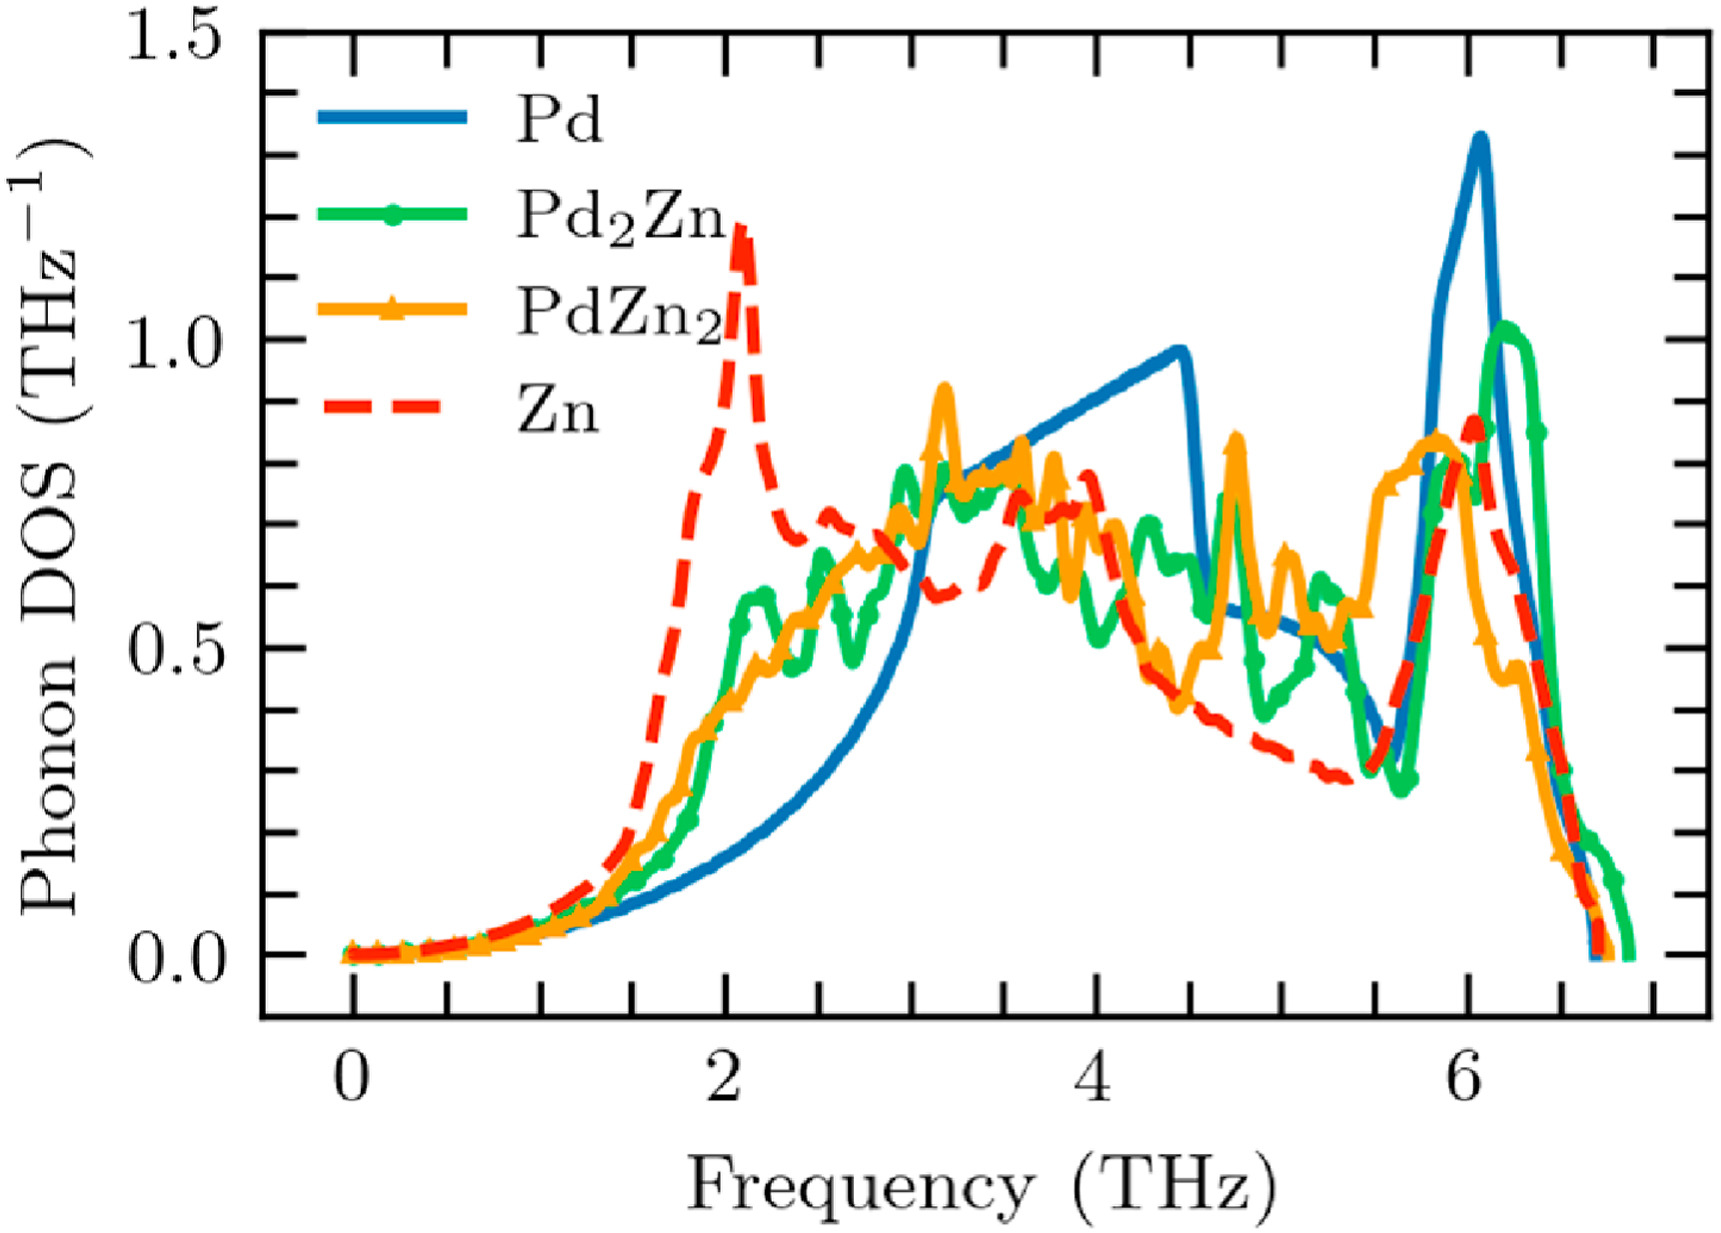
\includegraphics[width=0.5\textwidth]{intermetallics/Intermetallics-PdZnDOS.jpg}
    \caption{Predicted phonon DOS of Pd, Zn, Pd$_2$Zn and PdZn$_2$ from the DFT-based phonon calculations.}
    \label{intermetallics:fig:PdZnDOS}
\end{figure}

Figure \ref{intermetallics:fig:PdZnQHAPd} and Figure \ref{intermetallics:fig:PdZnQHAZn} show the comparison of the entropy and enthalpy of FCC-Pd and HCP-Zn from the phonon calculations to the SGTE pure element database \cite{dinsdale1991sgte}. Both show excellent agreement. For results of Pd obtained from phonon calculations and SGTE, the difference of enthalpy is less than 6.5\% and that of entropy is less than 5\%. The results of Zn show the difference of enthalpy less than 2.1\% and that of entropy less than 3.5\%.

\begin{figure}[H]
    \centering
    \normalsize
    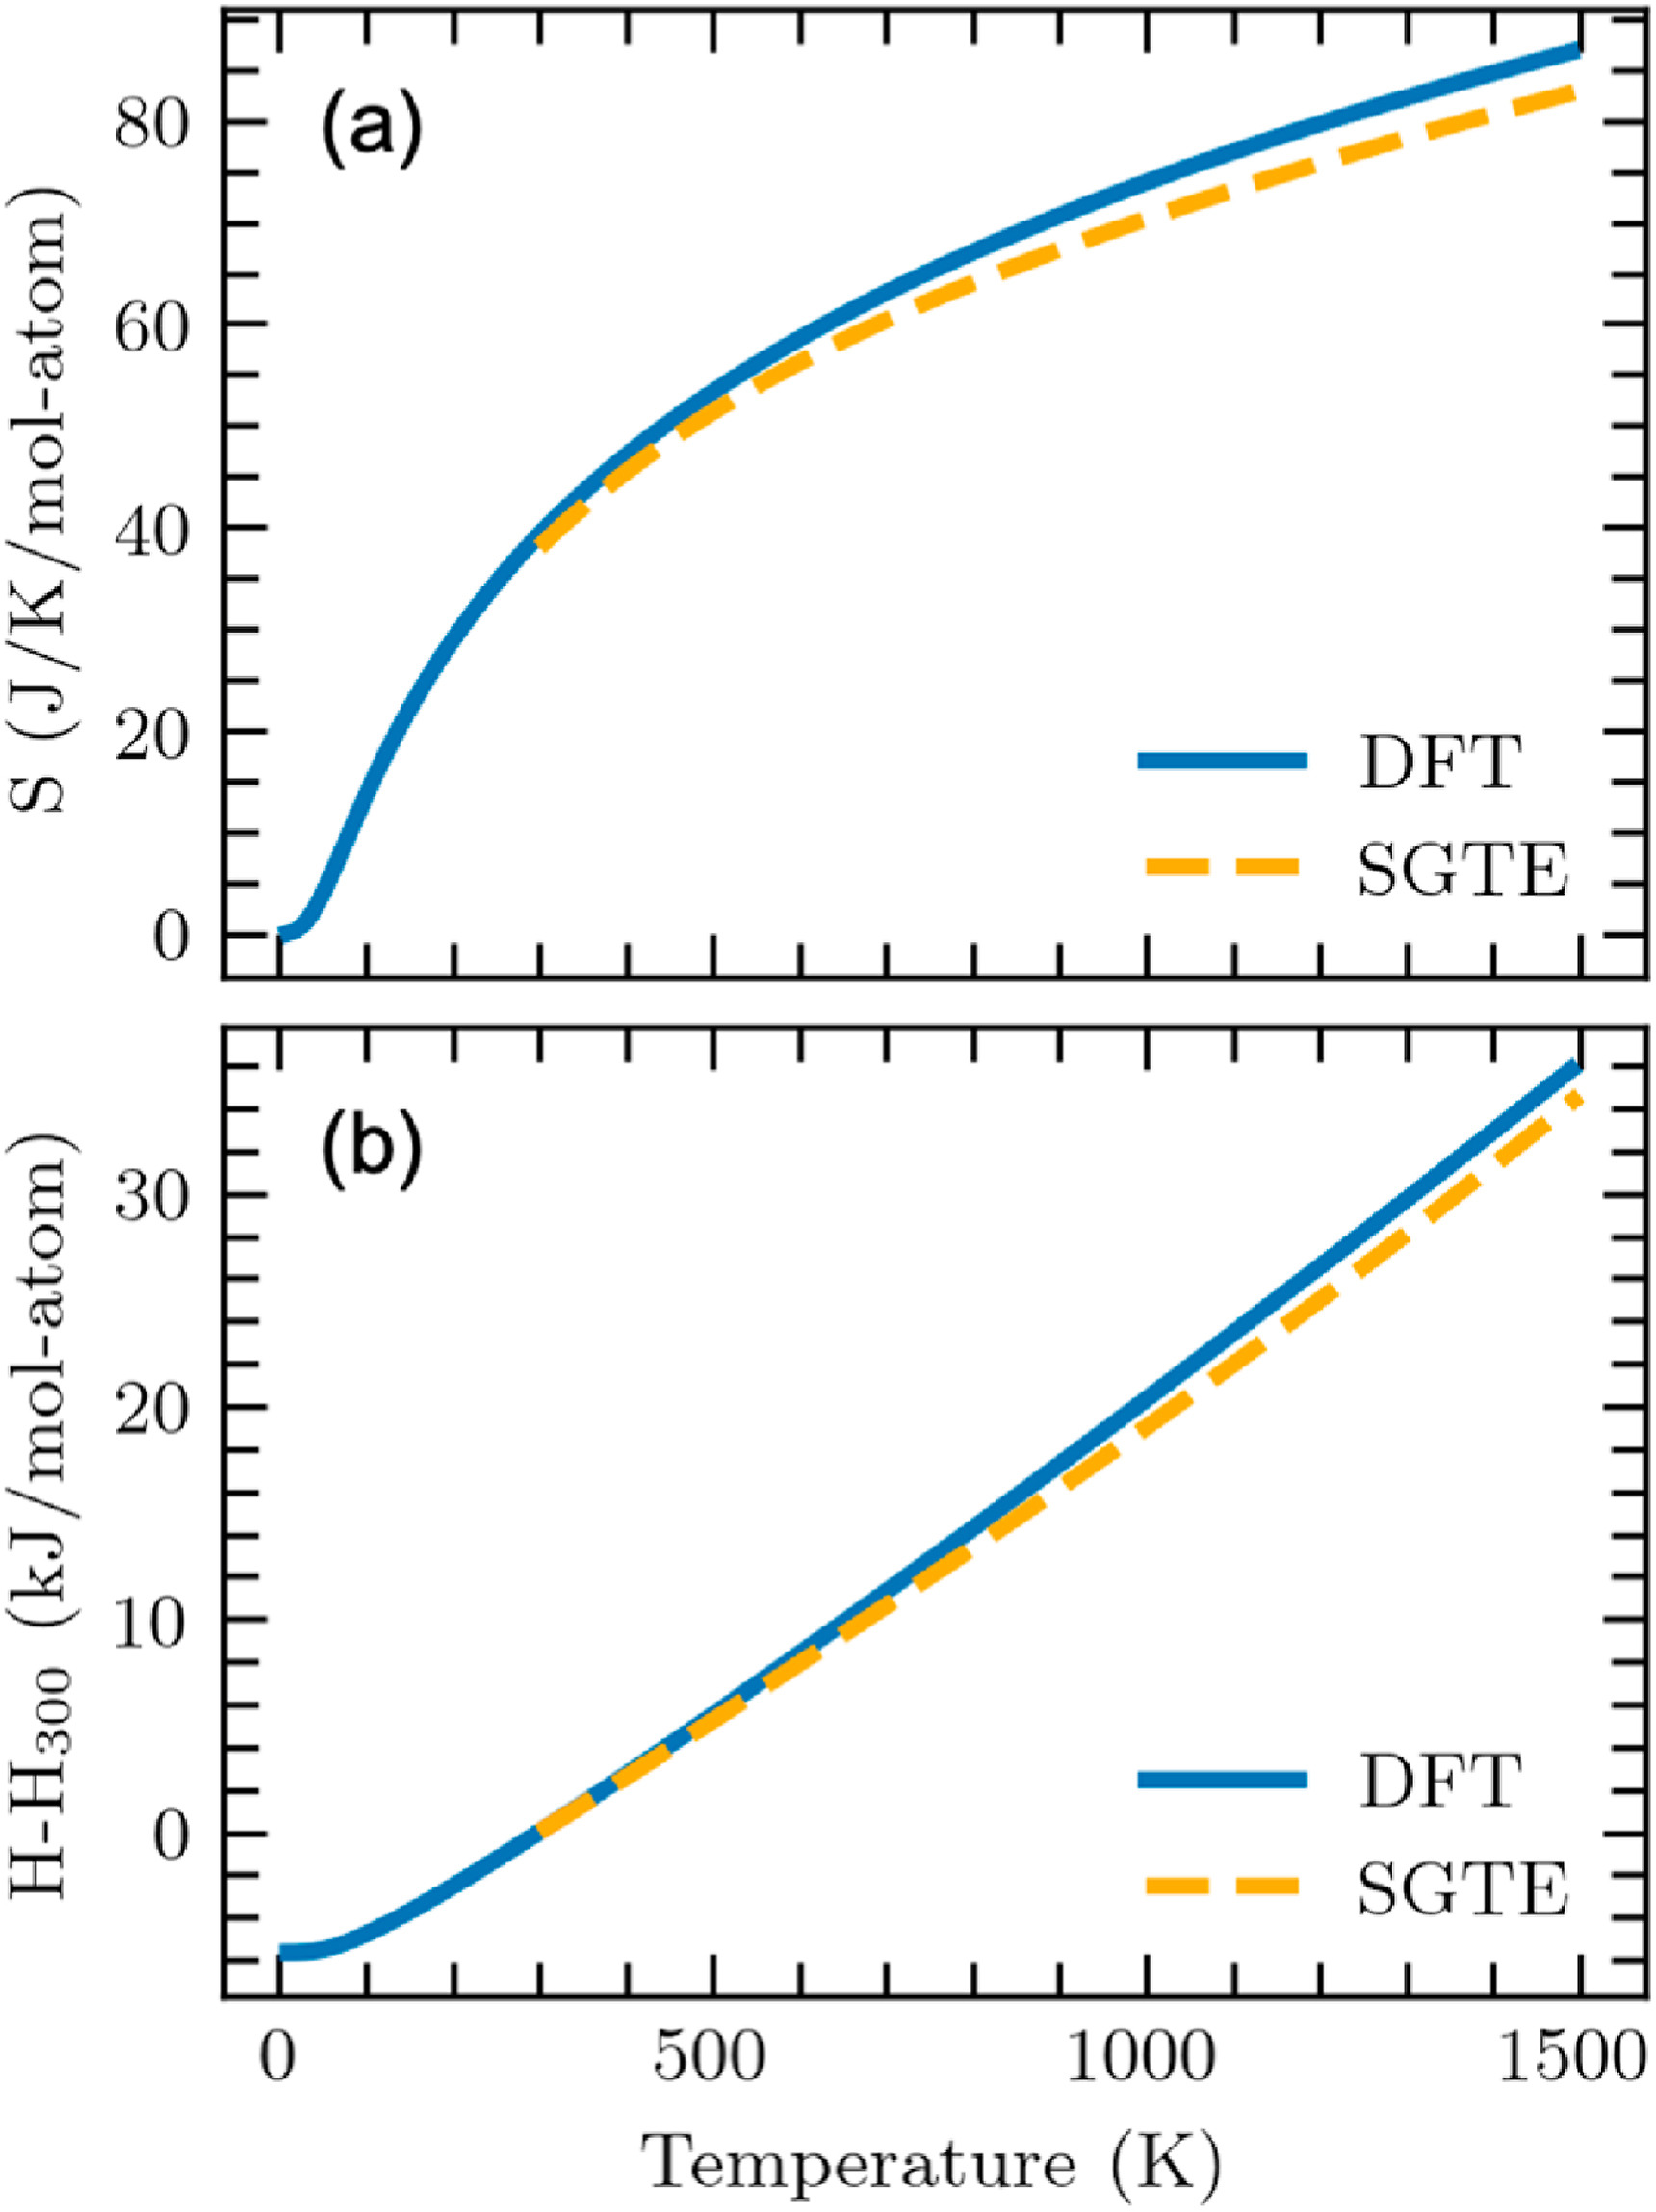
\includegraphics[width=0.4\textwidth]{intermetallics/Intermetallics-PdZnQHAPd.jpg}
    \caption{Comparison of the (a) entropy S and (b) enthalpy H $-$ H$_{300}$ of Pd from the DFT-based phonon calculations to the SGTE data \cite{dinsdale1991sgte}.}
    \label{intermetallics:fig:PdZnQHAPd}
\end{figure}

\begin{figure}[H]
    \centering
    \normalsize
    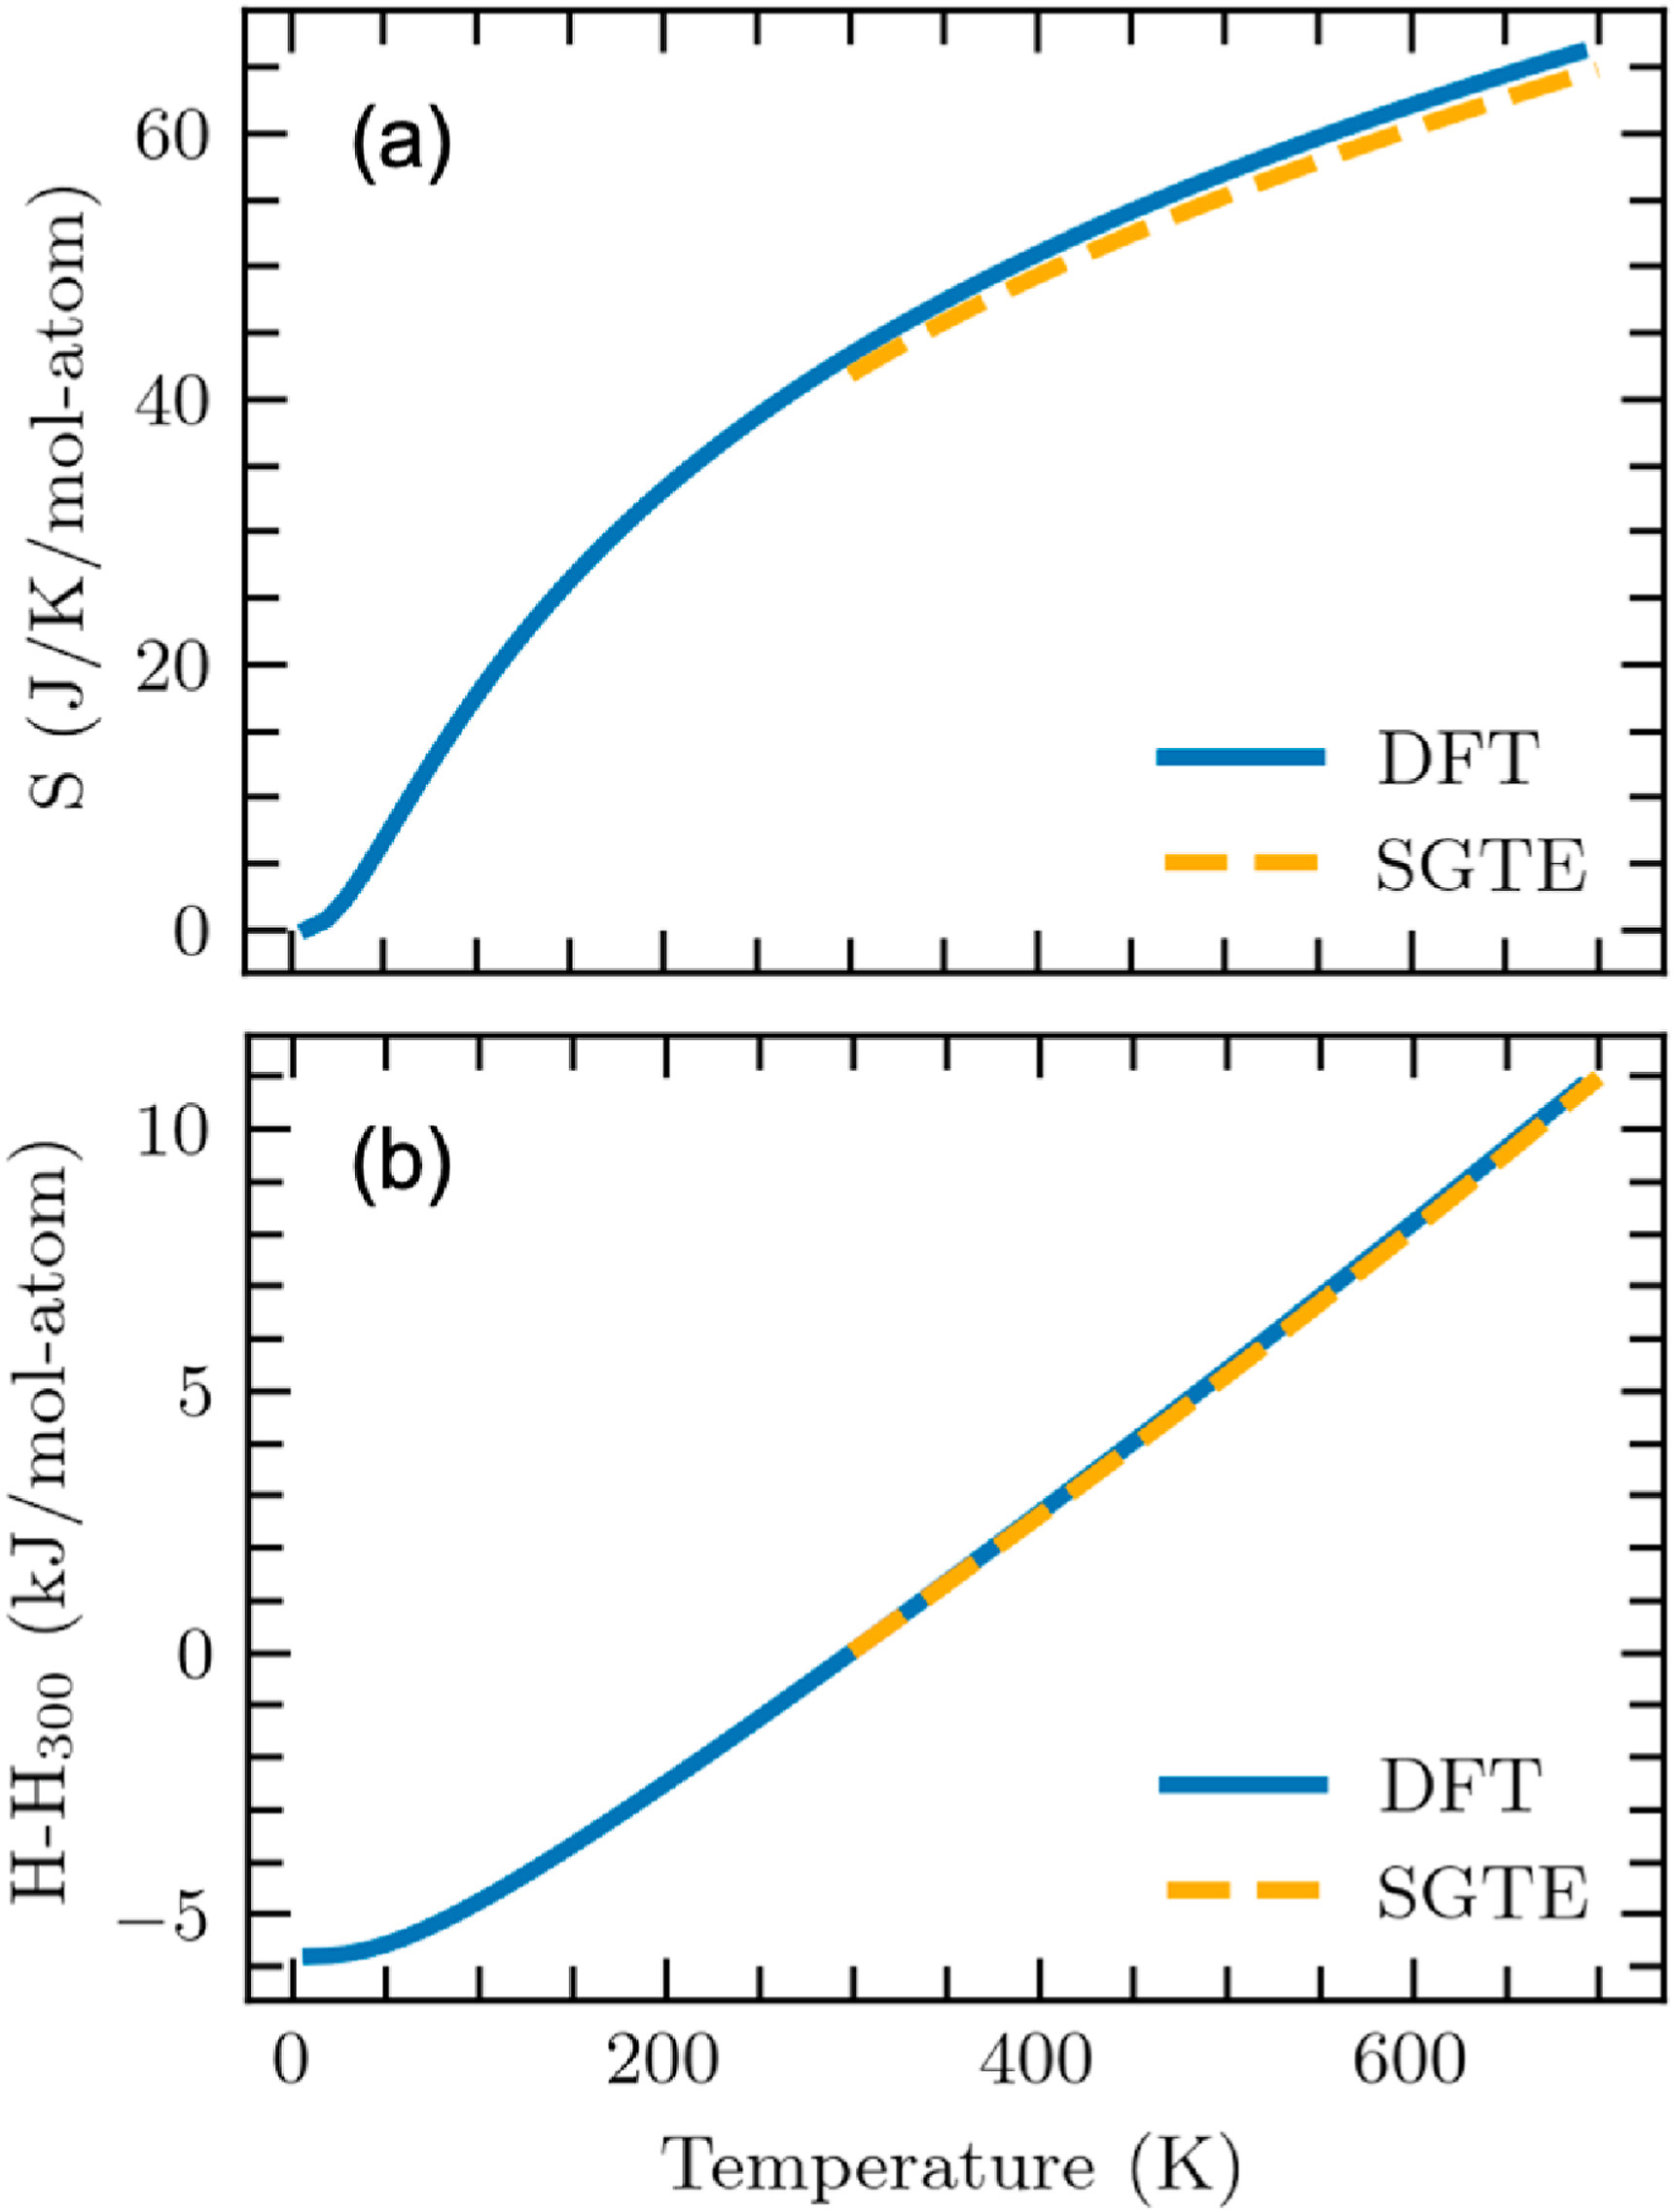
\includegraphics[width=0.4\textwidth]{intermetallics/Intermetallics-PdZnQHAZn.jpg}
    \caption{Comparison of the (a) entropy S and (b) enthalpy H $-$ H$_{300}$ of Zn from the DFT-based phonon calculations to the SGTE data \cite{dinsdale1991sgte}.}
    \label{intermetallics:fig:PdZnQHAZn}
\end{figure}

Table \ref{intermetallics:tab:PdZn_DFT_Hf} shows the enthalpy of formation $\Delta_f$H at 0 K predicted from the present DFT-based calculations using the exchange-correlation functionals of GGA and HSE06, along with experimental data \cite{ChiangIpserChang1977, kou1975thermodynamics}. For the $\gamma$-brass phase, the configuration of Pd$_{10}$Zn$_{42}$ ($x_{Zn}$ = 0.81) was used for DFT-based calculations and compared with experimental data at $x_{Zn}$ = 0.80. The $\Delta_f$H value predicted using HSE06 is $-33.7$ kJ/mol-atom, agreeing reasonably well with $-35.1$ kJ/mol-atom from experiments using calorimetry \cite{amore2009thermochemistry}. For the $\beta_1$ phase, the configuration of PdZn ($x_{Zn}$ = 0.50) was used. The $\Delta_f$H value of PdZn predicted using HSE06 is $-69.2$ kJ/mol-atom, which is in good agreement with measured $-73.9\pm10$ kJ/mol-atom reported by Chiang et al. \cite{ChiangIpserChang1977} and $-66.6$ kJ/mol-atom reported by Kou and Chang \cite{kou1975thermodynamics}, but is lower than the value predicted by GGA ($-53.7$ kJ/mol-atom). For both $\gamma$-brass and $\beta_1$ phases, the $\Delta_f$H values predicted by HSE06 are more accurate than those predicted by PBE-GGA. Considering the high computational cost, HSE06 was only applied for key endmembers close or on the convex hull in the present work such as (Zn)$_2$(Pd)$_3$(Pd)$_2$(Pd)$_6$ and (Zn)$_2$(Zn)$_3$(Pd)$_2$(Zn)$_6$. 

\begin{table}[H]
    \normalsize
    \centering
    \caption{Predicted enthalpy of formation at 0 K, $\Delta_f$H (kJ/mol-atom), of $\gamma$-brass and $\beta_1$ using DFT-based calculations with GGA and HSE06 as exchange-correlation functionals, respectively, in comparison with available experimental data.}
    \begin{tabular}{>{\raggedright\arraybackslash}m{2.5cm}>{\raggedright\arraybackslash}m{3cm}>{\raggedright\arraybackslash}m{2.5cm}>{\raggedright\arraybackslash}m{3cm}>{\raggedright\arraybackslash}m{3.5cm}}
    \hline
     \textbf{Phases} &  \textbf{Configurations} & \textbf{$x_{Zn}$} & \textbf{$\Delta_f$H} & \textbf{Source} \\
    \hline
    $\gamma$-brass phase & Pd$_{10}$Zn$_{42}$ & 0.81 & $-27.9$ & DFT/GGA\\
        & Pd$_{10}$Zn$_{42}$ & 0.81 & $-33.7$ & DFT/HSE06\\
       & N/A & 0.80 & $-35.1$ & Expt. at 300 K \cite{amore2009thermochemistry}\\
    $\beta_1$ phase & PdZn & 0.5 & $-53.7$ & DFT/GGA\\
       & PdZn & 0.5 & $-69.2$ & DFT/HSE06\\
       & PdZn & 0.5 & $-73.9\pm10$ & Expt. at 1273 K \cite{ChiangIpserChang1977}\\
       & PdZn & 0.5 & $-66.6$ & Expt. at 1273 K \cite{kou1975thermodynamics}\\
    \hline
    \end{tabular}
    \label{intermetallics:tab:PdZn_DFT_Hf}
\end{table}

\subsection{Thermodynamic modeling and phase equilibria} \label{intermetallics:ssec:PdZneq}
Figure \ref{Intermetallics:fig:PdZnPhaseDiagram} shows the calculated phase diagram in comparison with experimental data \cite{vizdal2006experimental, nowotny1951beitrag, alasafi1978mischung}, showing a good agreement, particularly the phase boundaries of the $\gamma$-brass phase. The max difference between calculated and experimental Zn compositions of the $\gamma$-brass phase  $x_{Zn}^{Cal}-x_{Zn}^{Expt.}$ is around 0.016 at 892 K. The solubility range of the $\gamma$-brass phase is between $x_{Zn} = 0.775 - 0.846$ from 300 K to 1000 K. The congruent melting temperature of the $\gamma$-brass phase is 1150 K in good agreement with 1153 K suggested by Massalski \cite{massalski1986binary}.\\

\begin{figure}[H]
    \centering
    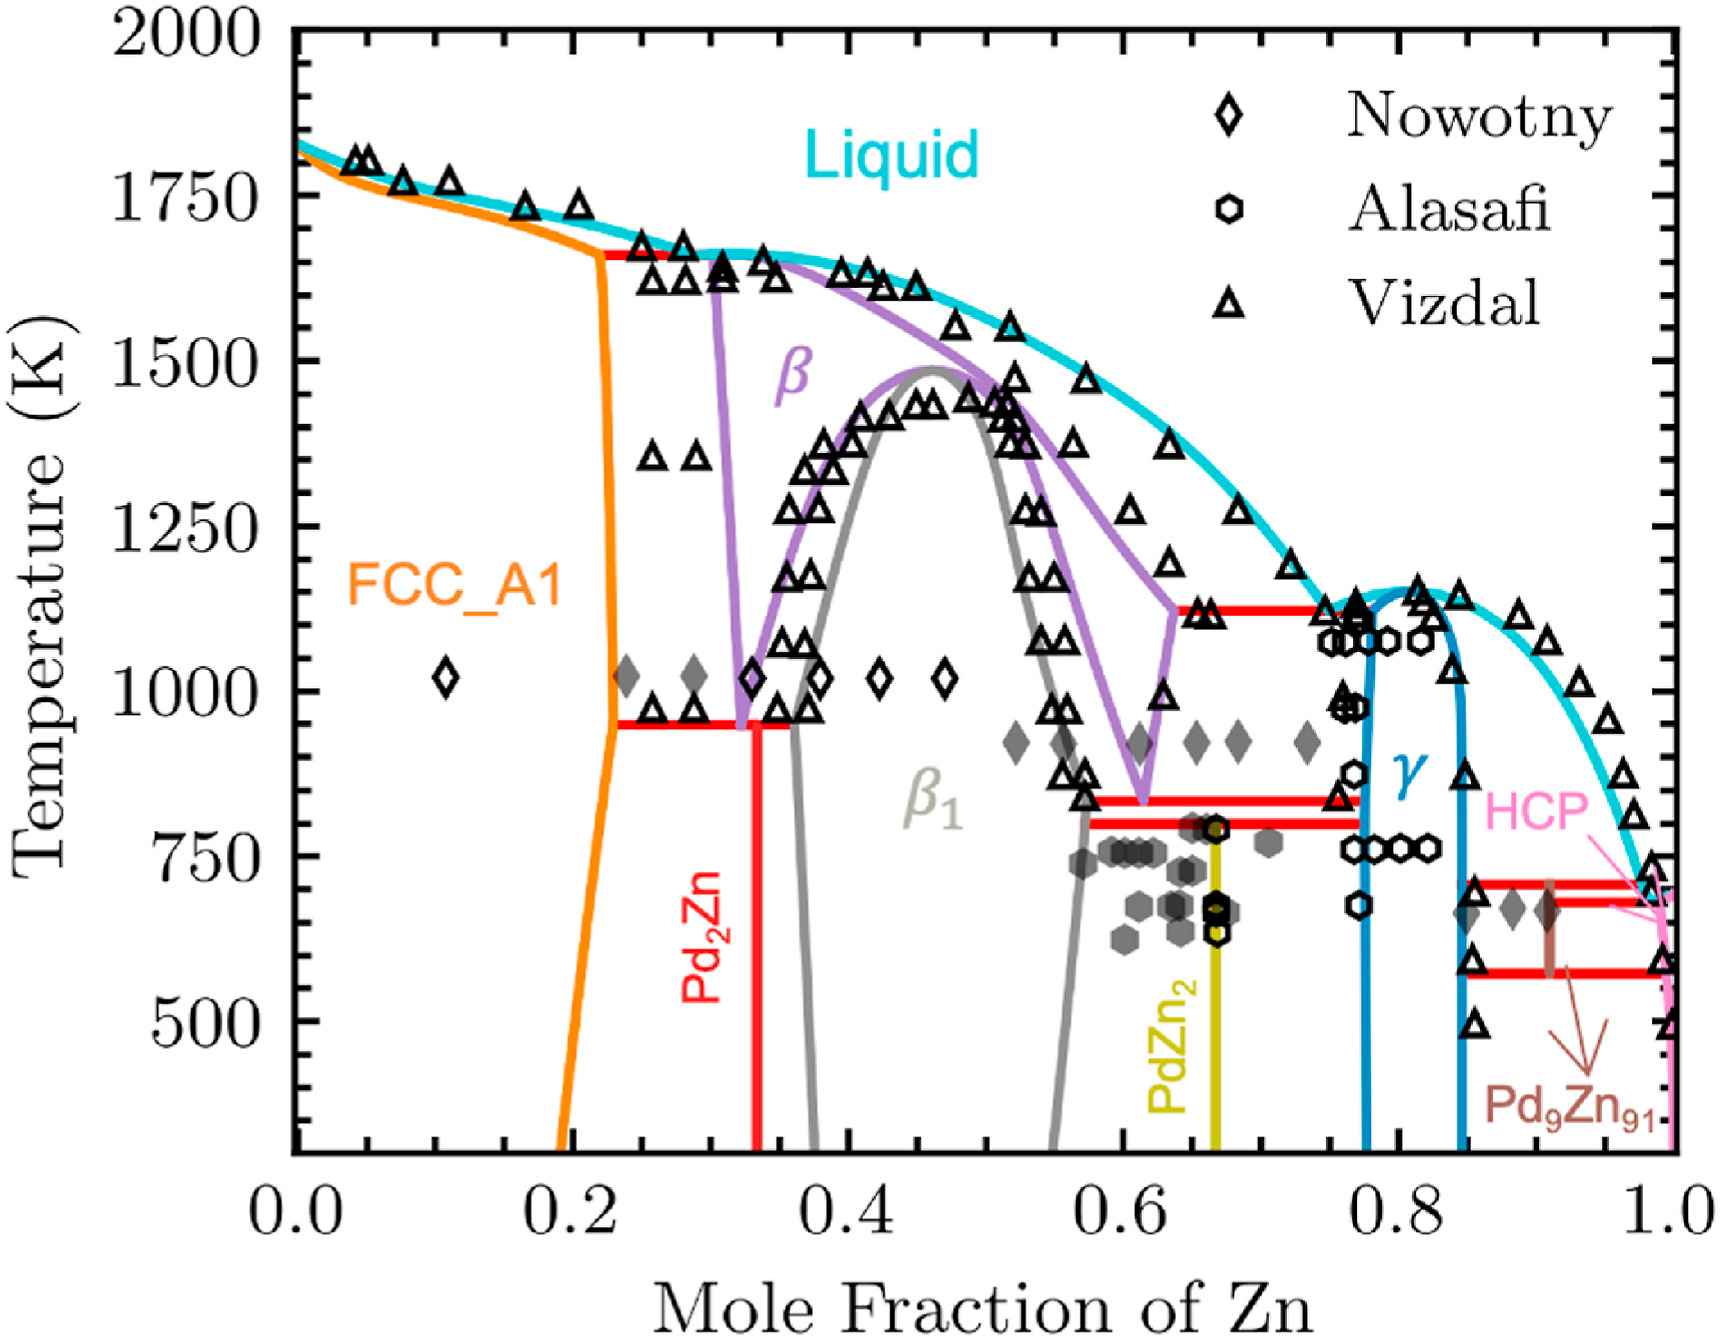
\includegraphics[width=0.6\linewidth]{intermetallics/Intermetallics-PdZnPhaseDiagram.jpg}
    \caption{Calculated phase diagram from the present CALPHAD modeling in comparison with experimental data from Nowotny et al. \cite{nowotny1951beitrag} (diamonds), Alasafi et al. \cite{alasafi1978mischung} (hexagons), and experimental data summarized by Vizdal et al. \cite{vizdal2006experimental} (triangles). Hollow diamonds and hexagons represent single phase region and shadowed diamonds and hexagons represent two phase regions reported by Nowotny et al. \cite{nowotny1951beitrag} and Alasafi et al. \cite{alasafi1978mischung}.}
    \label{Intermetallics:fig:PdZnPhaseDiagram}
\end{figure} 

\begin{table}[H]
    \centering
    \caption{Temperatures and compositions of invariant reactions in the Pd-Zn system calculated from the present CALPHAD modeling with available experimental data included.}
    \begin{tabular}{>{\raggedright\arraybackslash}m{5cm}>{\raggedright\arraybackslash}m{1cm}>{\raggedright\arraybackslash}m{1cm}>{\raggedright\arraybackslash}m{1cm}>{\raggedright\arraybackslash}m{3cm}>{\raggedright\arraybackslash}m{2.5cm}}
        \hline
         \textbf{Reaction}& \textbf{$x_{Zn}$} & (\%) &  & \textbf{Temperature (K)} & \textbf{Ref.}\\
        \hline
        Liquid $\rightarrow \beta + \gamma$&74.9&63.7&78.1&1122.1&This work\\
         &75&65&77&1118&Expt.\cite{massalski1986binary}\\
         $\beta \rightarrow \beta_1 + \gamma$&61.5&57.3&77.5&834&This work\\
	&57&55&76&838&Expt.\cite{massalski1986binary}\\
        $\beta_1 + \gamma \rightarrow$ PdZn$_2$&57.2&77.5&66.7&799.6&This work\\
	&56&76&66.7&$803\pm10$&Expt.\cite{massalski1986binary}\\
        Liquid $+ \gamma \rightarrow$ Pd$_9$Zn$_{91}$&97.7&84.6&91.0&707.2&This work\\
	&98&85&92&703&Expt.\cite{hansen1958constitution}\\
	&&&&707&Expt.\cite{vizdal2006experimental}\\
        Liquid $\rightarrow$ Pd$_9$Zn$_{91}$ $+$ HCP&98.2&91.0&99.0&681.1&This work\\
	&&&&690&Expt.\cite{vizdal2006experimental}\\
         \hline
    \end{tabular}
    \label{intermetallics:tab:inv}
\end{table}

Table \ref{intermetallics:tab:inv} lists the temperatures and compositions of invariant reactions. The experimentally reported invariant reactions, i.e., Liquid $\rightarrow$ Pd$_9$Zn$_{91}$ $+$ HCP by Vizdal et al. \cite{vizdal2006experimental} and other four invariant reactions by Massalski \cite{massalski1986binary}, are well reproduced. The largest discrepancy is seen for the eutectic reaction, Liquid $\rightarrow$ Pd$_9$Zn$_{91}$ + HCP, i.e., 681 K calculated from the present work versus 690 K in the literature \cite{vizdal2006experimental}.

\begin{figure}[H]
    \centering
    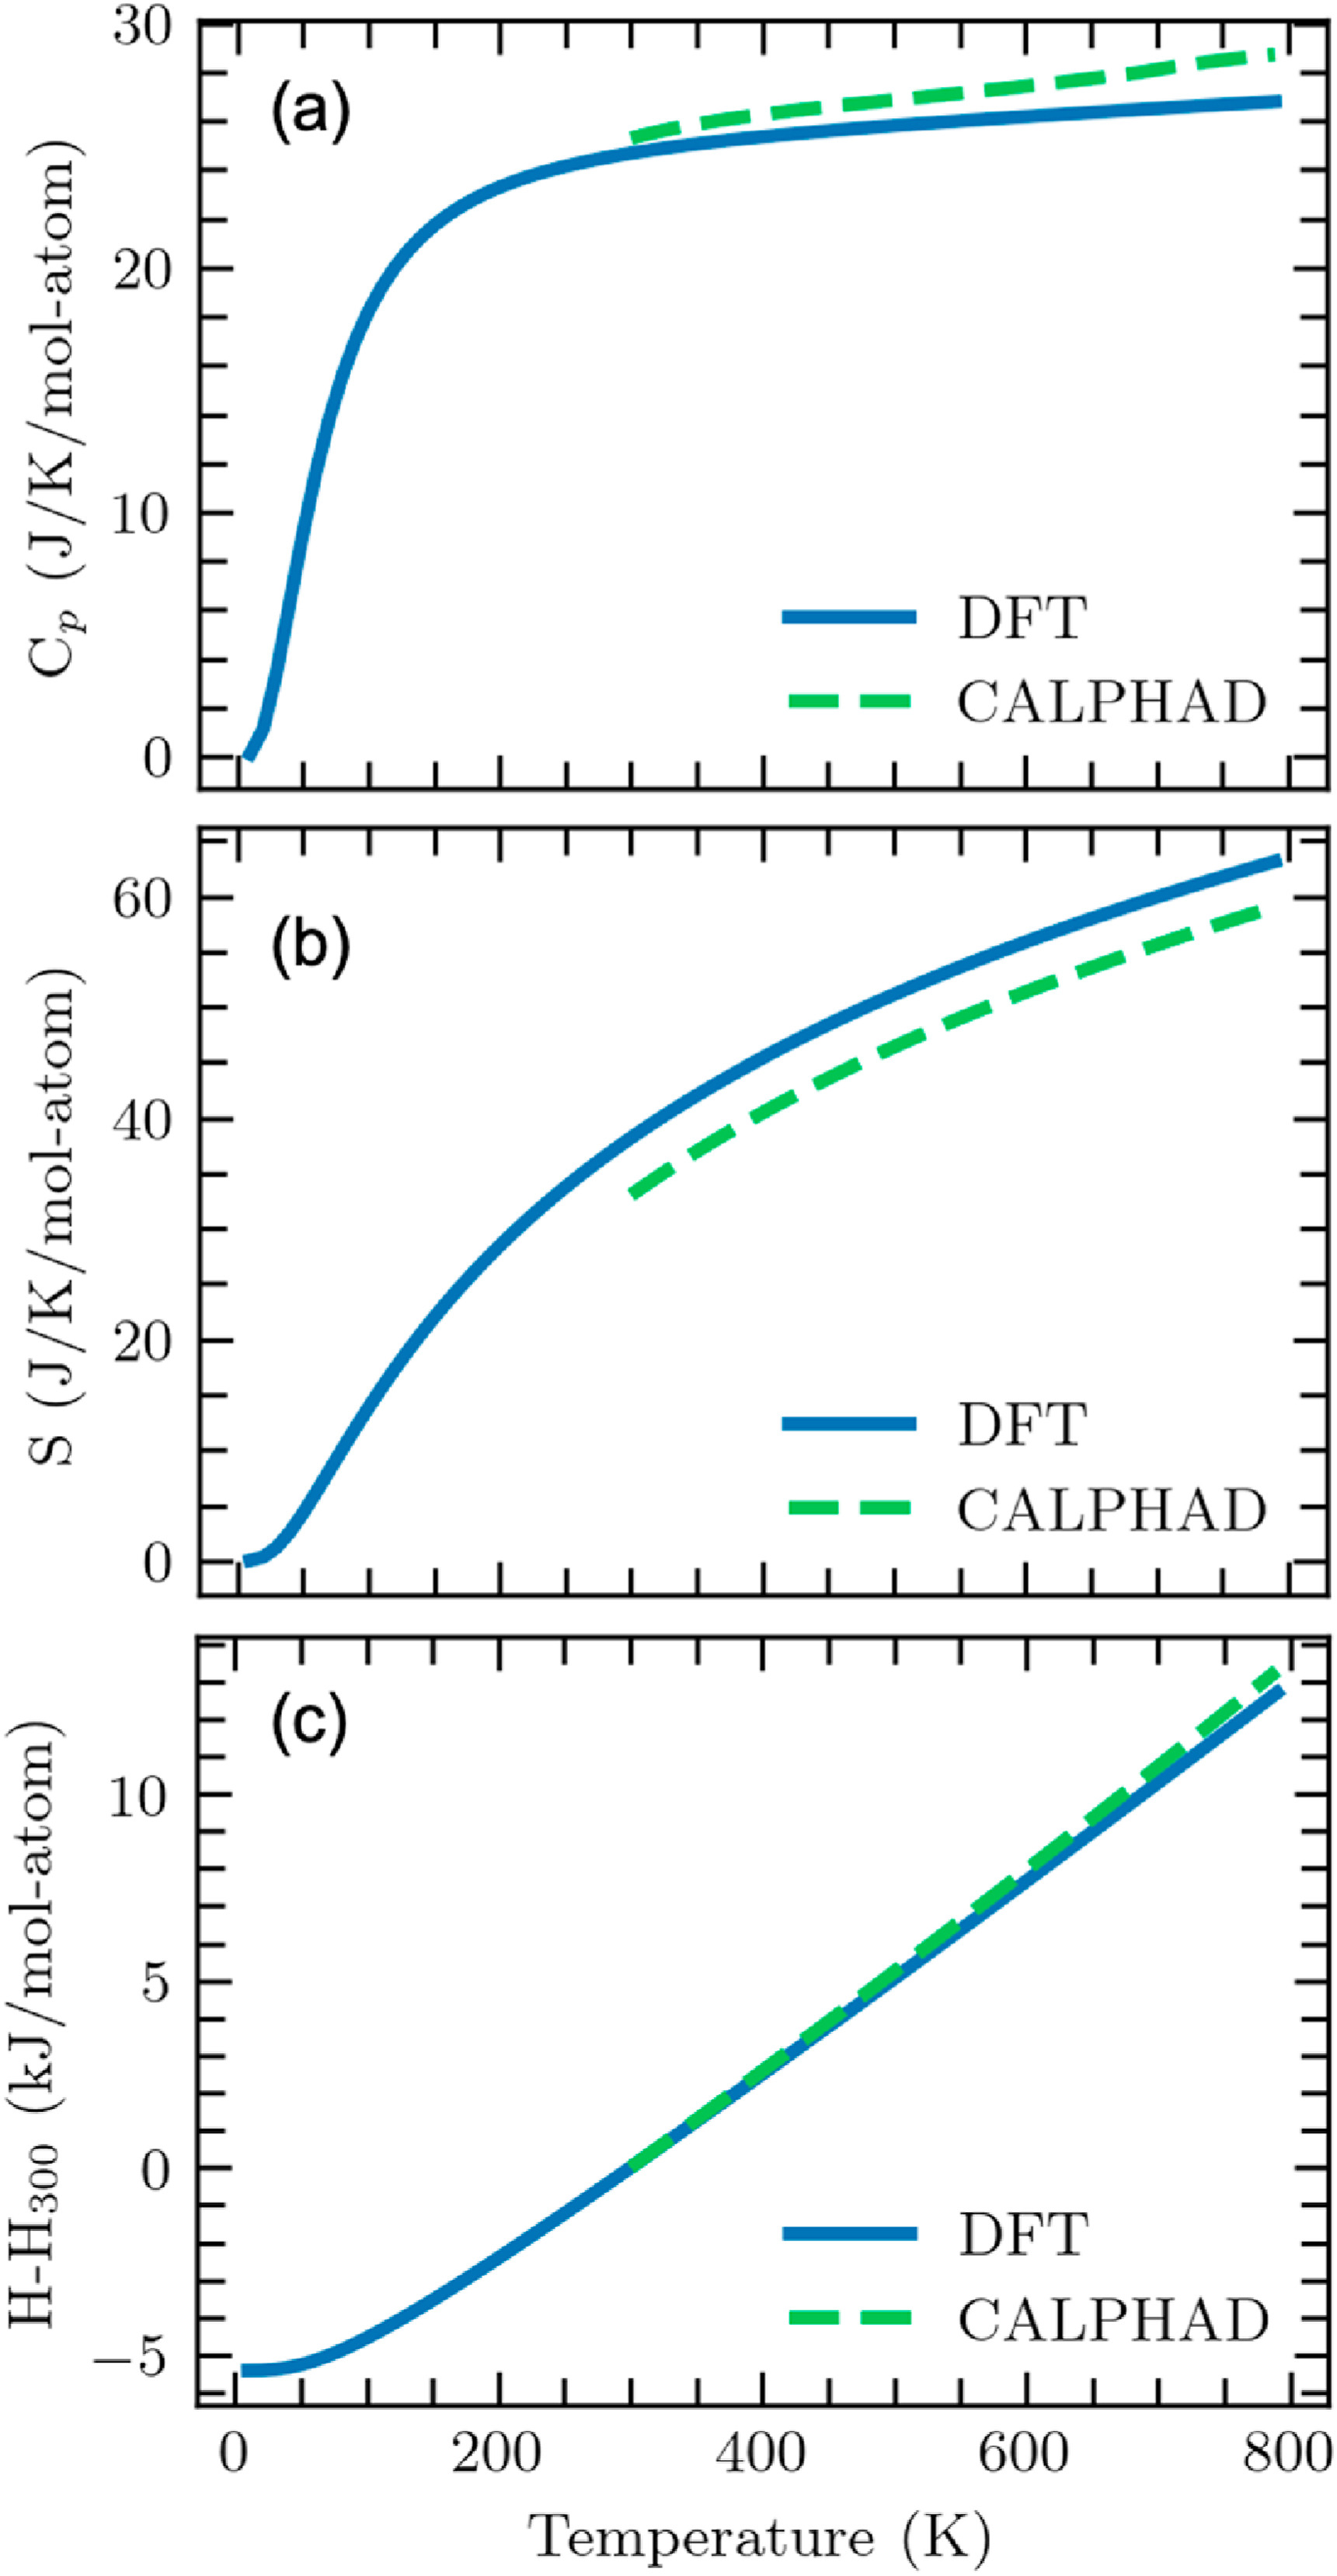
\includegraphics[width=0.45\linewidth]{intermetallics/Intermetallics-PdZnQHAPd2Zn.jpg}
    \caption{Predicted (a) heat capacity C$_p$, (b) entropy S, and (c) enthalpy H $-$ H$_{300}$ of Pd$_2$Zn using the present results form DFT-based phonon calculations, compared with those from the present CALPHAD modeling.}
    \label{intermetallics:fig:PdZnQHAPd2Zn}
\end{figure}

Figure \ref{intermetallics:fig:PdZnQHAPd2Zn} and Figure \ref{intermetallics:fig:PdZnQHAPdZn2} show the heat capacity, entropy, and enthalpy of stoichiometric compounds Pd$_2$Zn and PdZn$_2$ from the present model in comparison with results from the phonon calculations. Good agreement is found, especially for enthalpy with a difference less than 4.7\% for Pd$_2$Zn and 2.8\% for PdZn$_2$. The entropy of PdZn$_2$ from phonon calculations compared with the present model shows the largest discrepancy with a difference of around 6.5 J/mol-atom-K. This is because the model parameters of stoichiometric compounds, which are obtained from first-principles calculated enthalpy and entropy, were adjusted with the experimental data of the peritectoid temperature.

\begin{figure}[H]
    \centering
    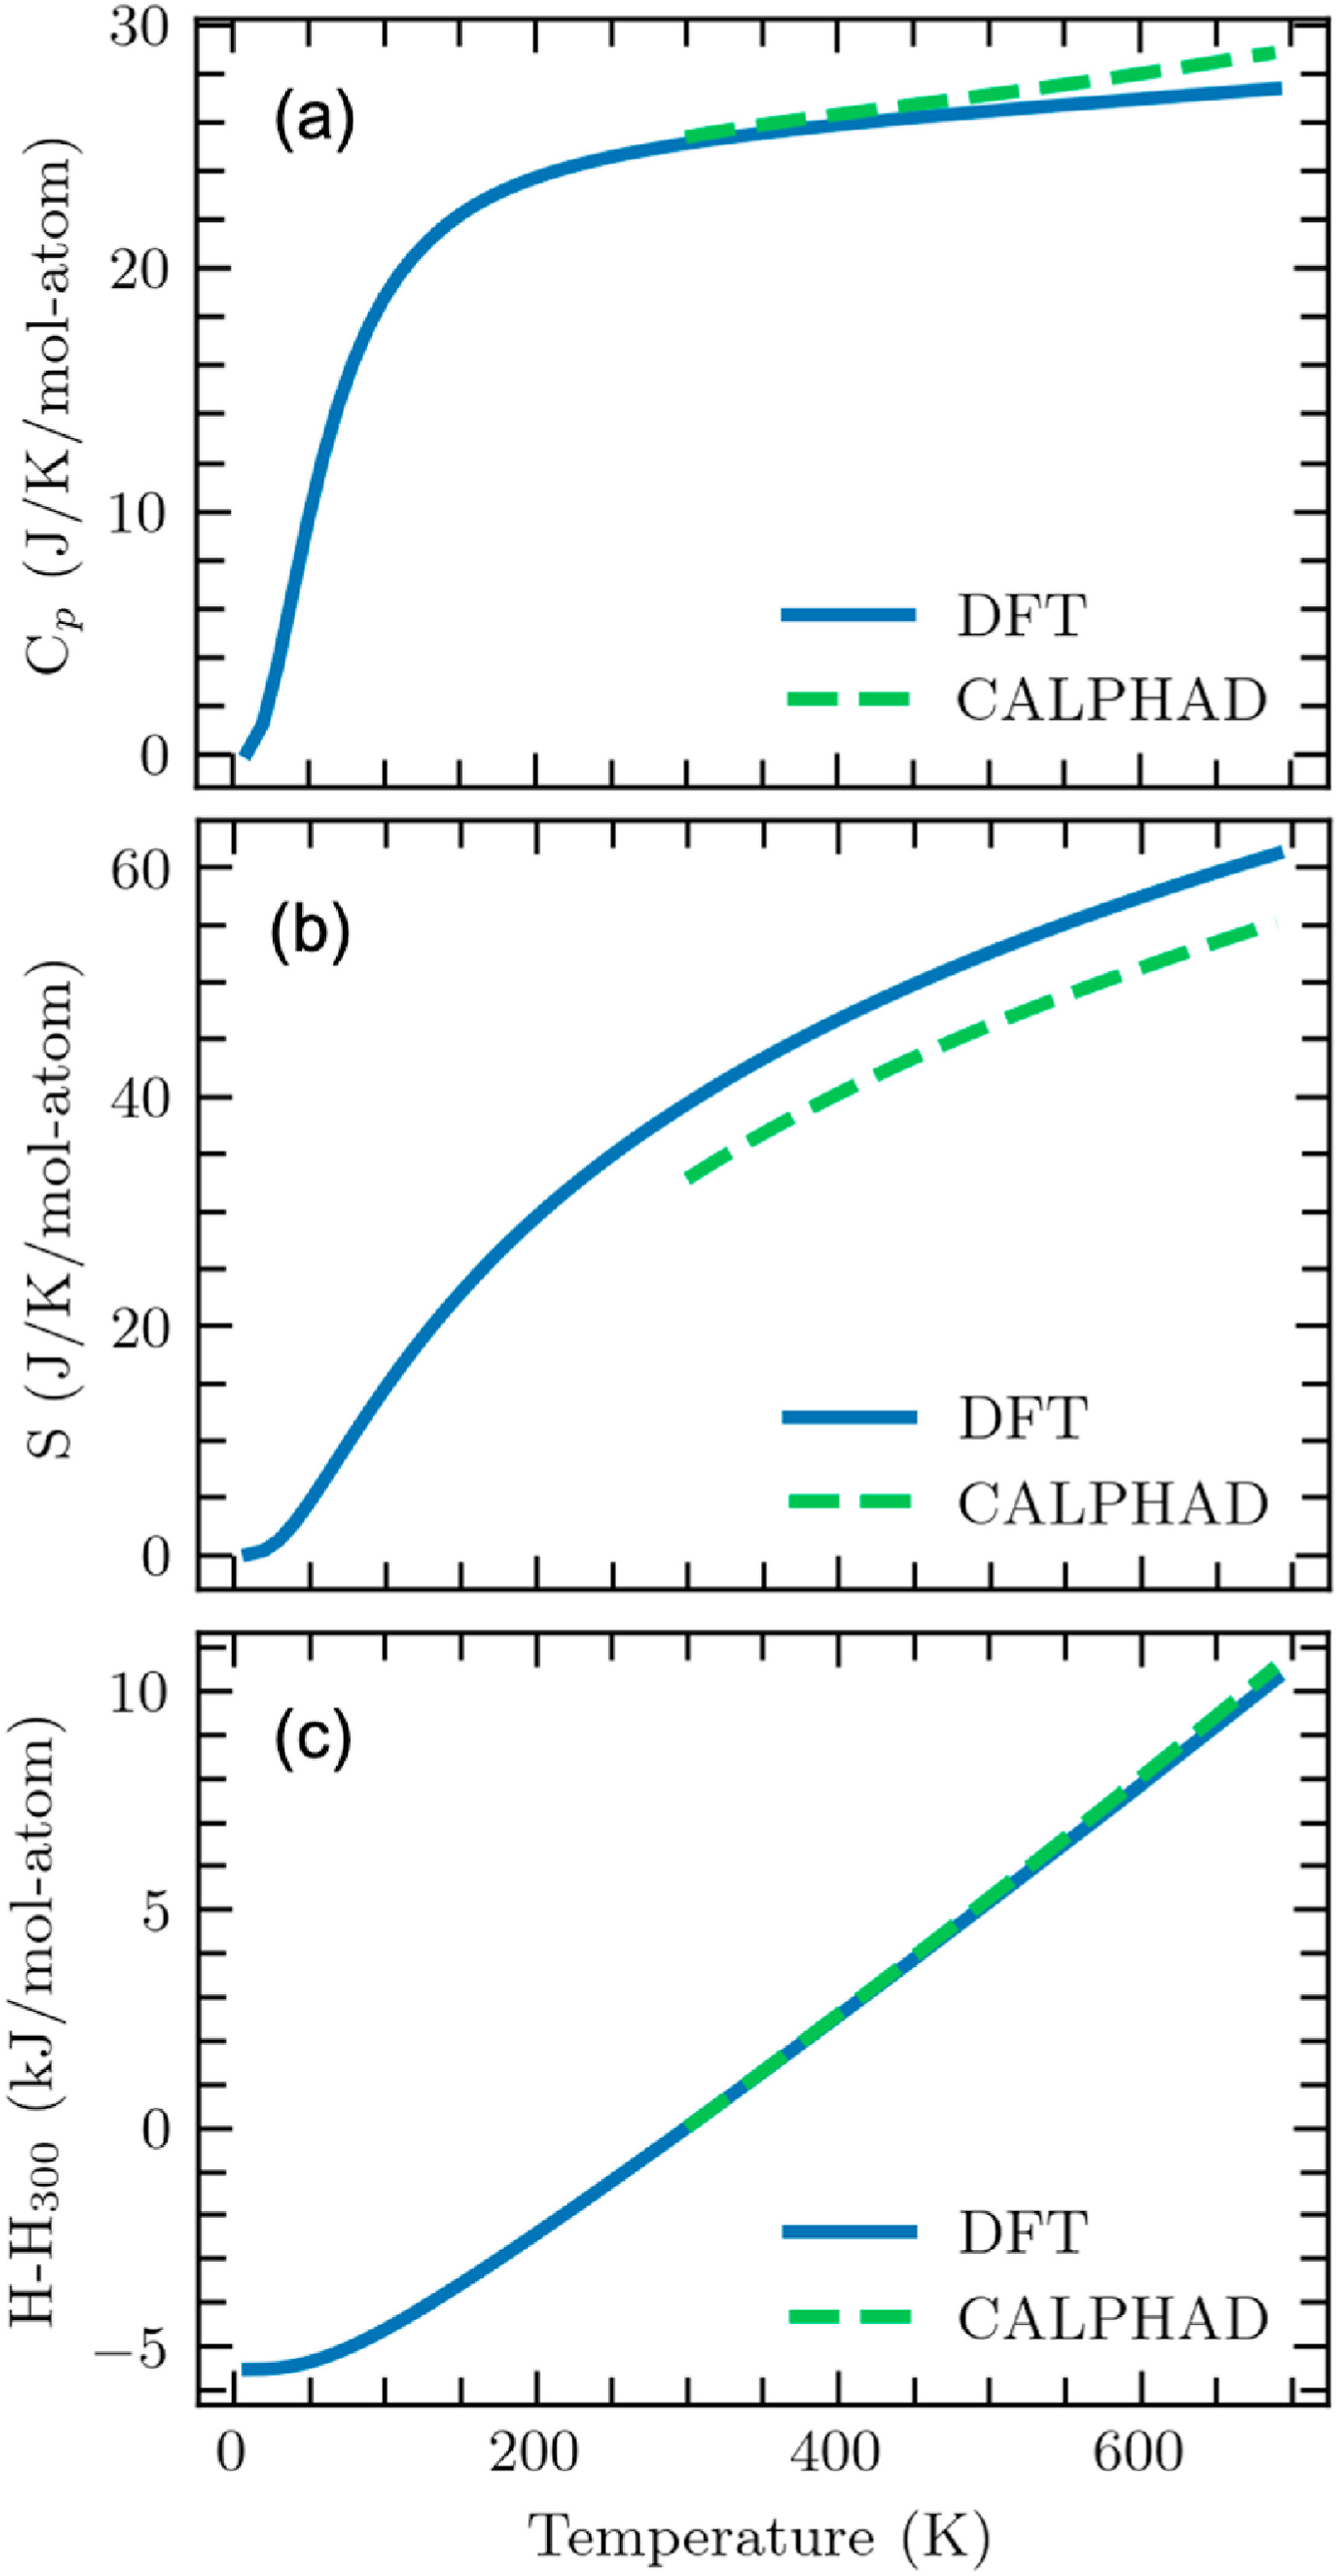
\includegraphics[width=0.45\linewidth]{intermetallics/Intermetallics-PdZnQHAPdZn2.jpg}
    \caption{Predicted (a) heat capacity C$_p$, (b) entropy S, and (c) enthalpy H $-$ H$_{300}$ of PdZn$_2$ using the present results form DFT-based phonon calculations, compared with those from the present CALPHAD modeling.}
    \label{intermetallics:fig:PdZnQHAPdZn2}
\end{figure}

The parameters of the FCC\_A1 phase in the database were optimized based on phase boundary data and activity data of the FCC\_A1 phase. Considering fitting different types of data, a balanced modeling result between phase boundary data and activity data is chosen. The experimental data for liquidus and solidus on the Pd-rich side are scarce. In the present work, data for liquidus and solidus in the Pd-rich side summarized by Vizdal et al. \cite{vizdal2006experimental} are used for modeling, thus the shape of liquidus and solidus in the Pd-rich side followed the trend of experimental data. Figure \ref{intermetallics:fig:PdZnACR} shows the activity values of Zn at 1273 K calculated from the present model in comparison with experimental data by Chiang et al. \cite{ChiangIpserChang1977}. The activity values of Zn in $\beta_1$ from the present model agree well with the experiments \cite{ChiangIpserChang1977} with the mean absolute error of $\ln{a_{Zn}}$ being 0.4. A higher discrepancy occurs in the composition range $x_{Zn}$ = 0.51-0.6. For example, at $x_{Zn}$ = 0.55, $\ln{a_{Zn}}$ calculated from the present model is $-3.52$ compared with -1.56 measured by Chiang et al. \cite{ChiangIpserChang1977}. They reported a single $\beta_1$ phase for $x_{Zn}$ = 0.52 and a single $\beta$ phase for $x_{Zn}$ = 0.6. However, the present work predicts that $\beta_1$ is in equilibrium with $\beta$ at $x_{Zn}$ = 0.52, and $\beta$ is in equilibrium with Liquid at $x_{Zn}$=0.6 (see Figure \ref{Intermetallics:fig:PdZnPhaseDiagram}). Figure \ref{intermetallics:fig:PdZnACRUQ} shows the activity values of Zn in FCC, $\beta$, and $\beta_1$ phases, respectively, calculated from the present model with the shaded regions for the uncertainty of each phase. For FCC, larger uncertainty occurs when $x_{Zn}$ < 0.2, where the largest uncertainty is around $\pm15$\% from the mean value at $x_{Zn}$ = 0.02, and experimental data are located within this uncertainty region. For $\beta_1$, the experimental data are in the uncertainty region when $x_{Zn}$ < 0.5, and the largest error is around $x_{Zn}$ = 0.52 with $\ln{a_{Zn}}$ = $-1.66$ from experiments \cite{ChiangIpserChang1977} compared with $-3.35$ calculated from the present model. For $\beta$, $\ln{a_{Zn}} = -10.33$ from experiments \cite{ChiangIpserChang1977} at $x_{Zn}$ = 0.3 are closer to the lower limit of the uncertainty region, where $\ln{a_{Zn}}$ at the lower uncertainty is $-10.81$. The shaded ranges in Figure \ref{intermetallics:fig:PdZnACRUQ} decrease with increasing $x_{Zn}$, indicating a larger uncertainty of activity occurs in the Pd-rich region. 

\begin{figure}[H]
    \centering
    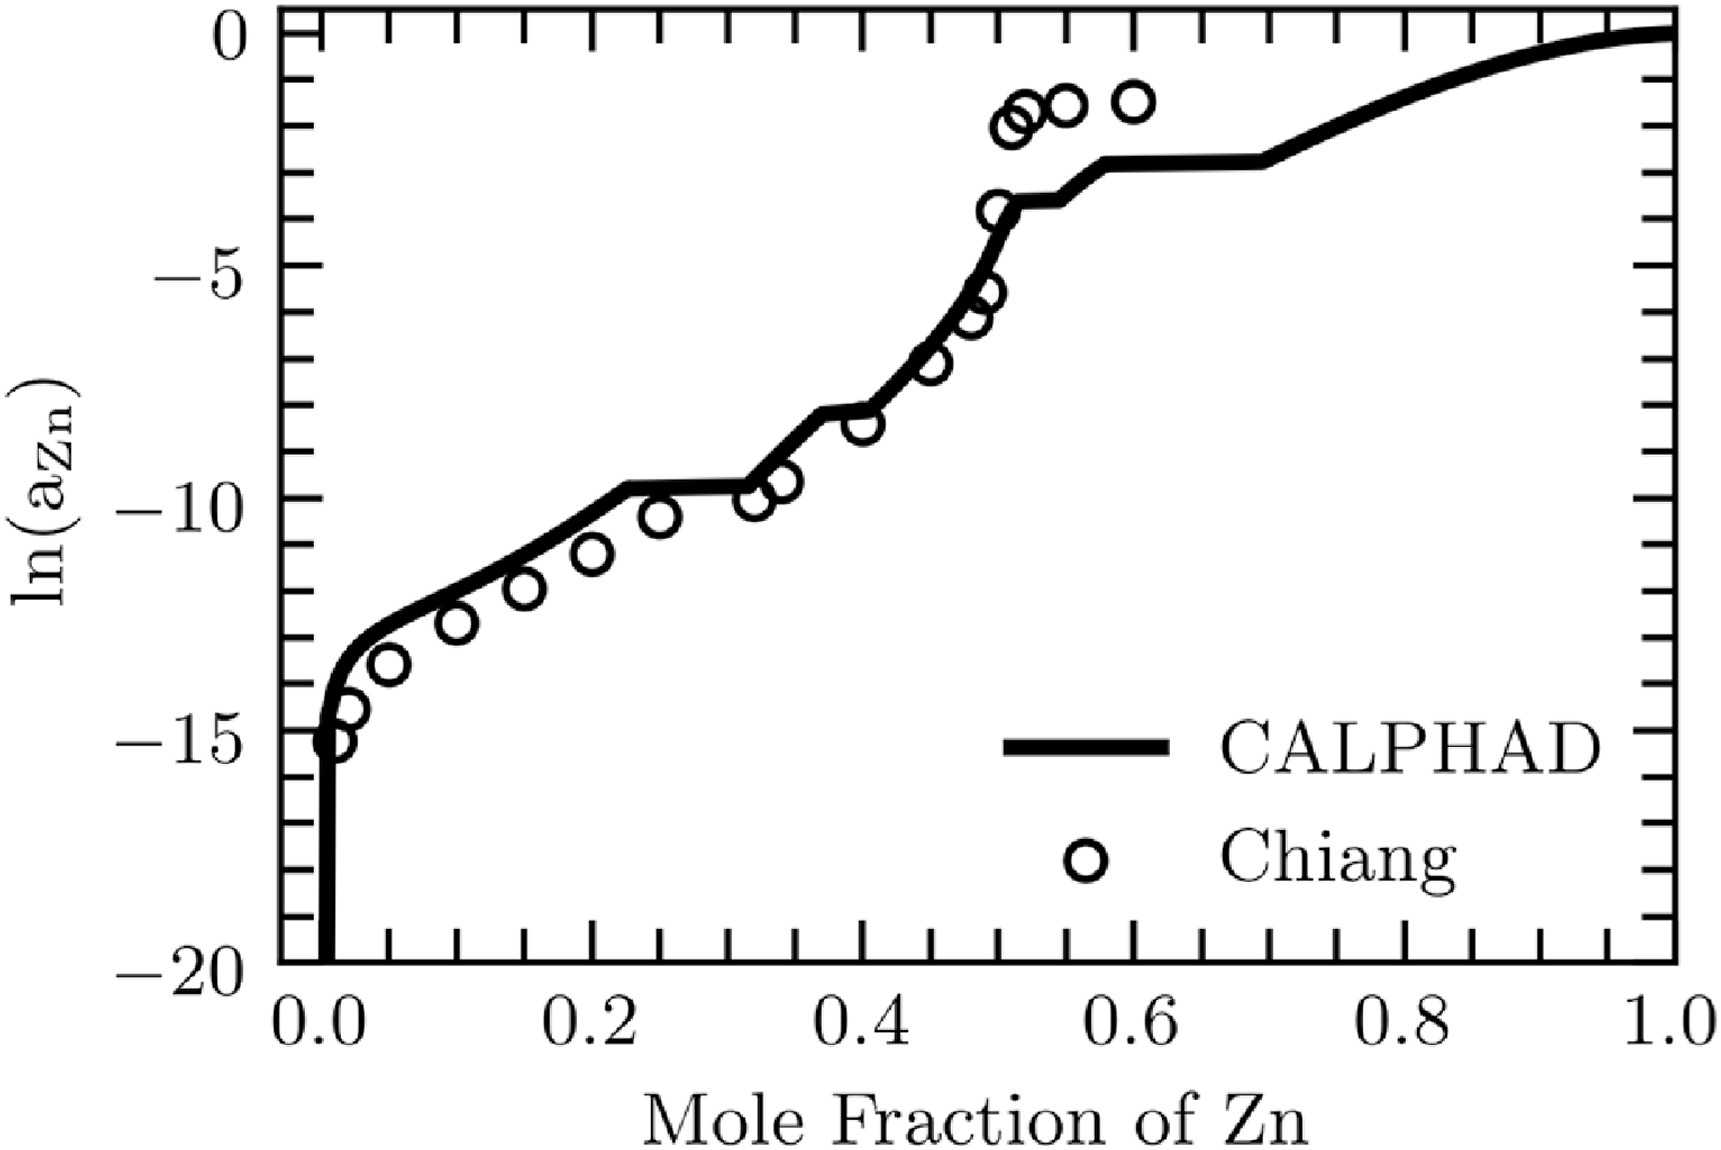
\includegraphics[width=0.5\linewidth]{intermetallics/Intermetallics-PdZnACR.jpg}
    \caption{Calculated activity of Zn at 1273 K with experimental data measured by Chiang et al. \cite{ChiangIpserChang1977} superimposed.}
    \label{intermetallics:fig:PdZnACR}
\end{figure}

\begin{figure}[H]
    \centering
    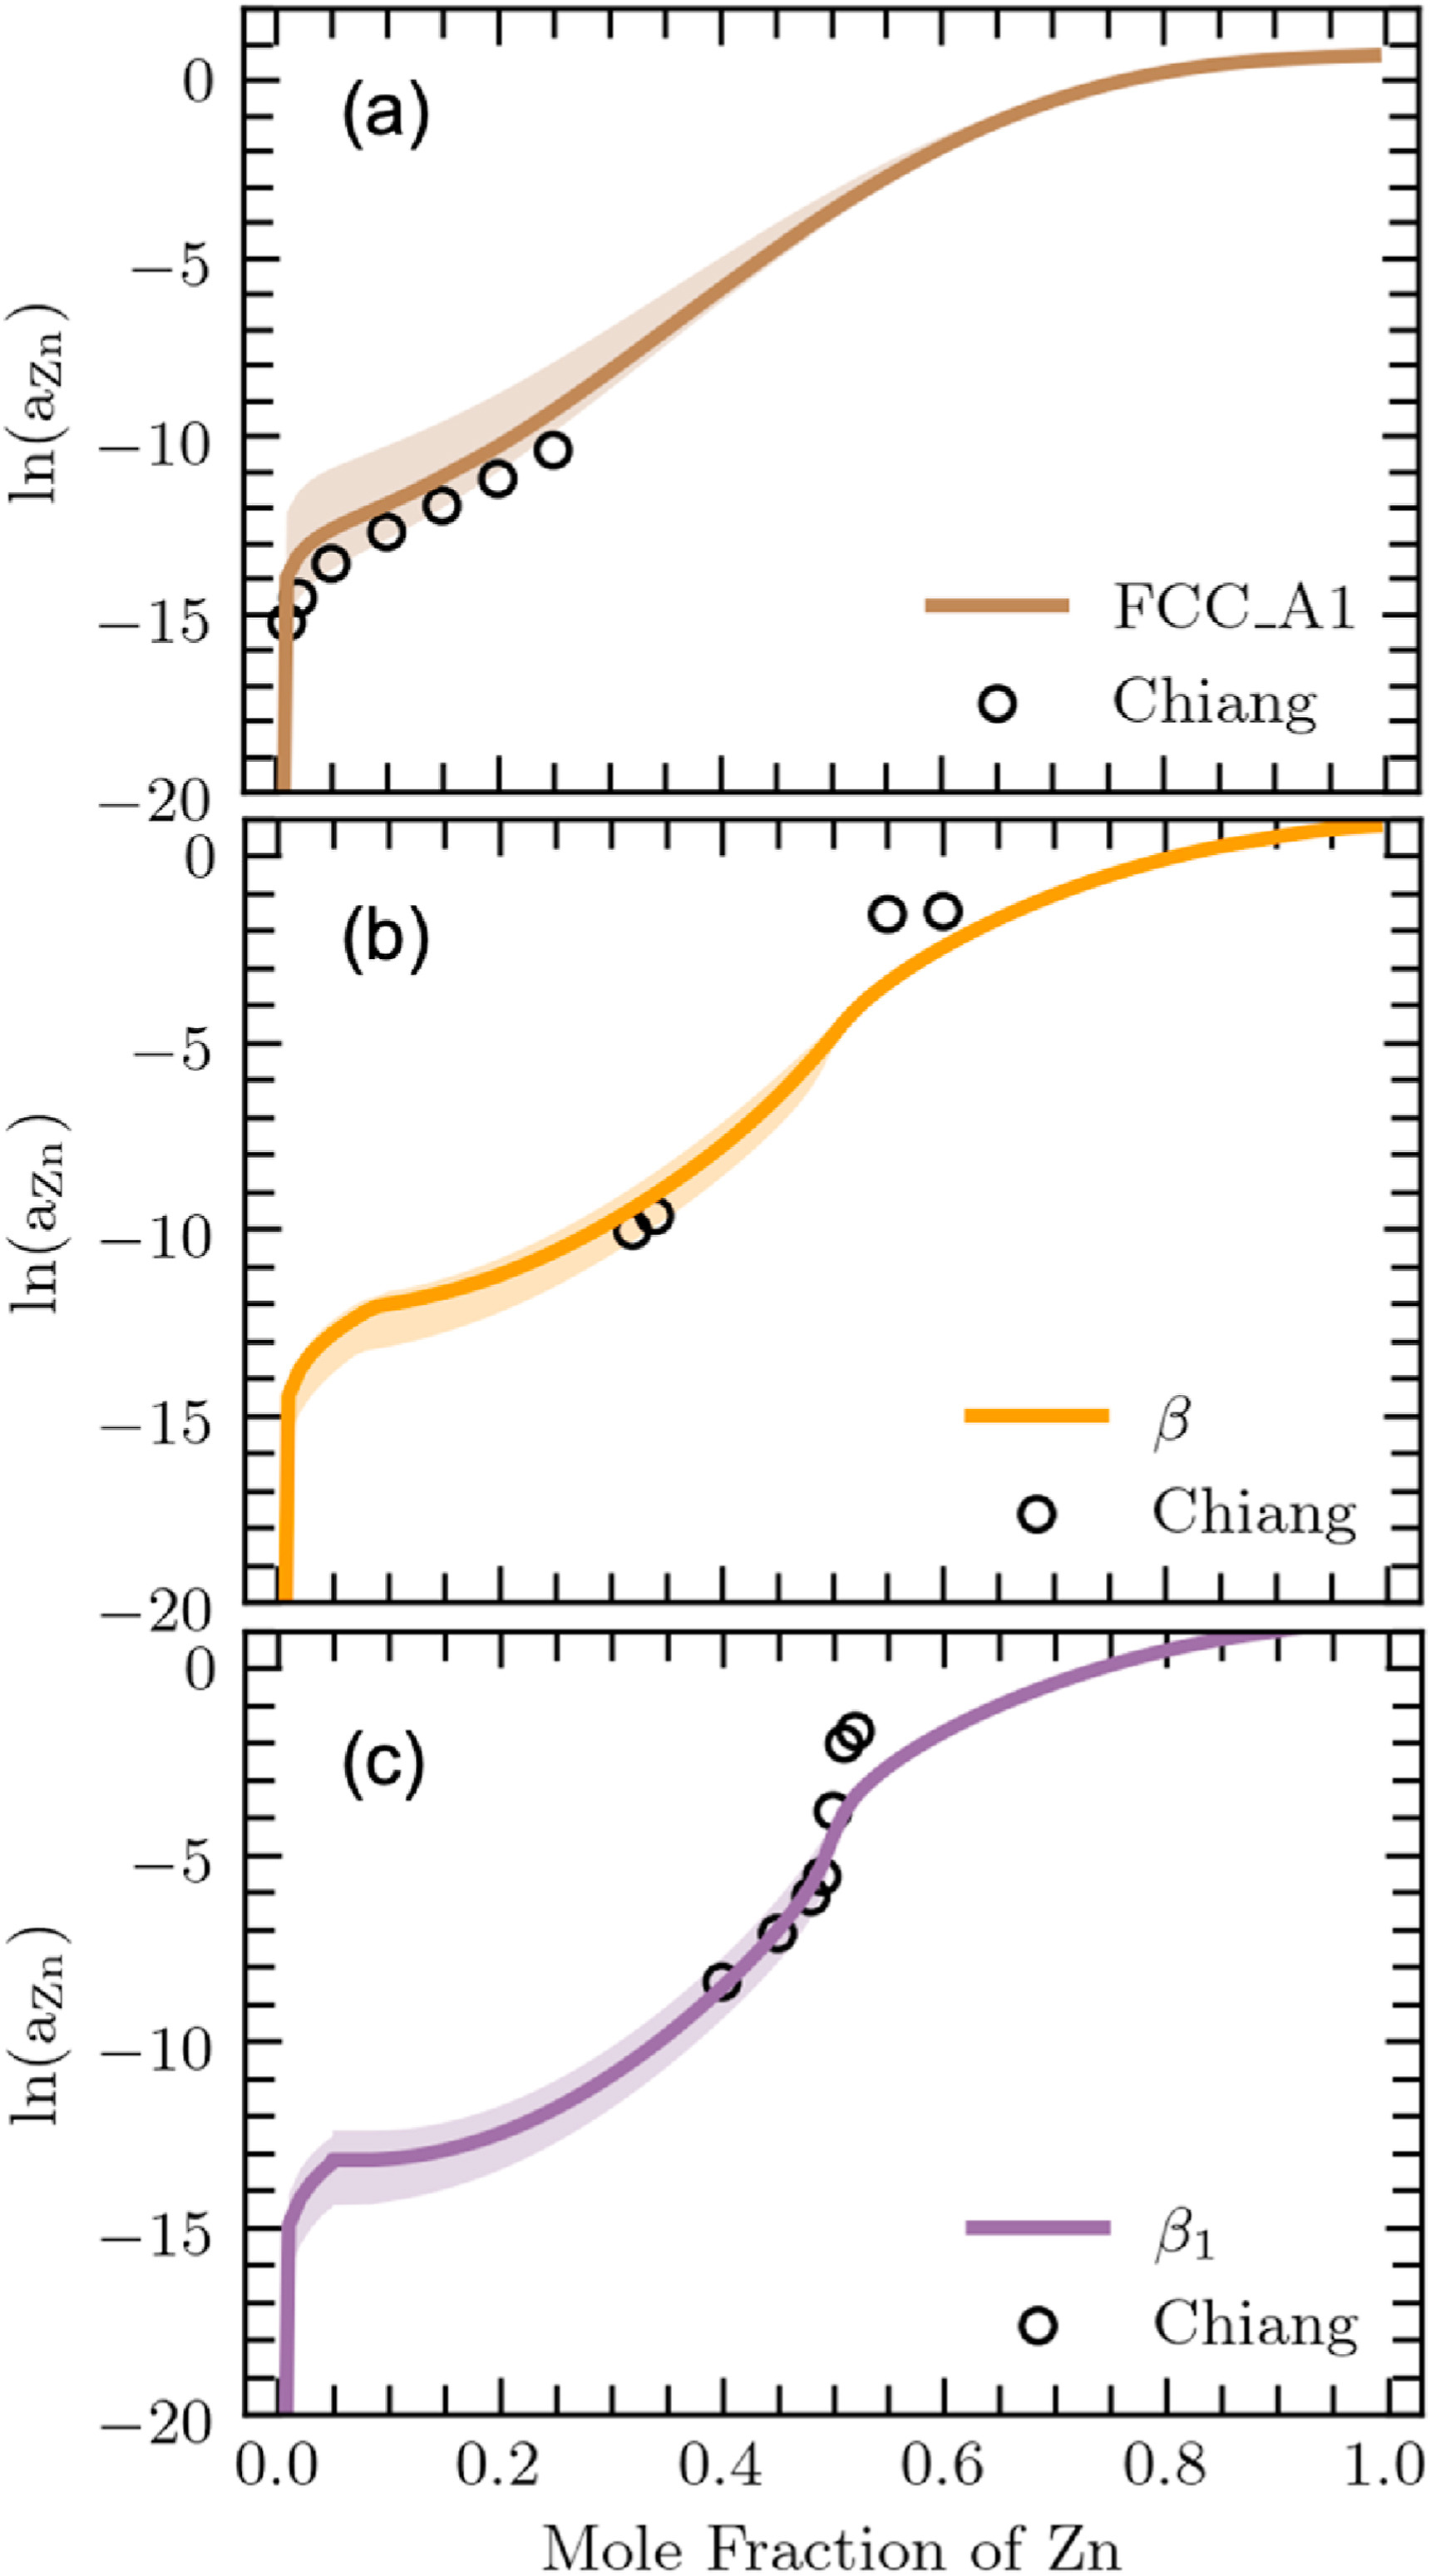
\includegraphics[width=0.5\linewidth]{intermetallics/Intermetallics-PdZnACRUQ.jpg}
    \caption{Uncertainty quantification of the activity of (a) FCC, (c) $\beta$, and (d) $\beta_1$, marked in the shaded regions with the corresponding color of each phase and compared with experimental data by Chiang et al. \cite{ChiangIpserChang1977}.}
    \label{intermetallics:fig:PdZnACRUQ}
\end{figure}

Figure \ref{intermetallics:fig:PdZnHMR} plots the enthalpy of formation $\Delta_f$H of the Pd-Zn phases at 1273 K and 300 K from the present model and available experimental data \cite{amore2009thermochemistry, ChiangIpserChang1977, kou1975thermodynamics}, along with the calculated results from the previous CALPHAD modeling \cite{vizdal2006experimental} at 300 K and the present first-principles results of the $\gamma$-brass phase at 0 K and high temperatures. $\Delta_f$H at 1273 K agrees reasonably well with experimental data \cite{ChiangIpserChang1977, kou1975thermodynamics}. $\Delta_f$H of $\beta_1$ at $x_{Zn}$ = 0.5 and 1273 K is $-70.1$ kJ/mol-atom from the present work, compared with -$73.9\pm10$ kJ/mol-atom measured by Chiang et al. \cite{ChiangIpserChang1977} and $-66.6$ kJ/mol-atom measured by Kou et al. \cite{kou1975thermodynamics}. Figure \ref{intermetallics:fig:PdZnHMR} shows that $\Delta_f$H of $\gamma$-brass from the present model has better agreement with experiments than the previous model \cite{vizdal2006experimental}. At $x_{Zn}$ = 0.8, $\Delta_f$H value of $\gamma$-brass from the present model is $-40.6$ kJ/mol-atom at 300 K and from the previous model \cite{vizdal2006experimental} is $-48.5$ kJ/mol-atom, compared with $-35.1$ kJ/mol-atom measured by Amore et al. \cite{amore2009thermochemistry}.

\begin{figure}[H]
    \centering
    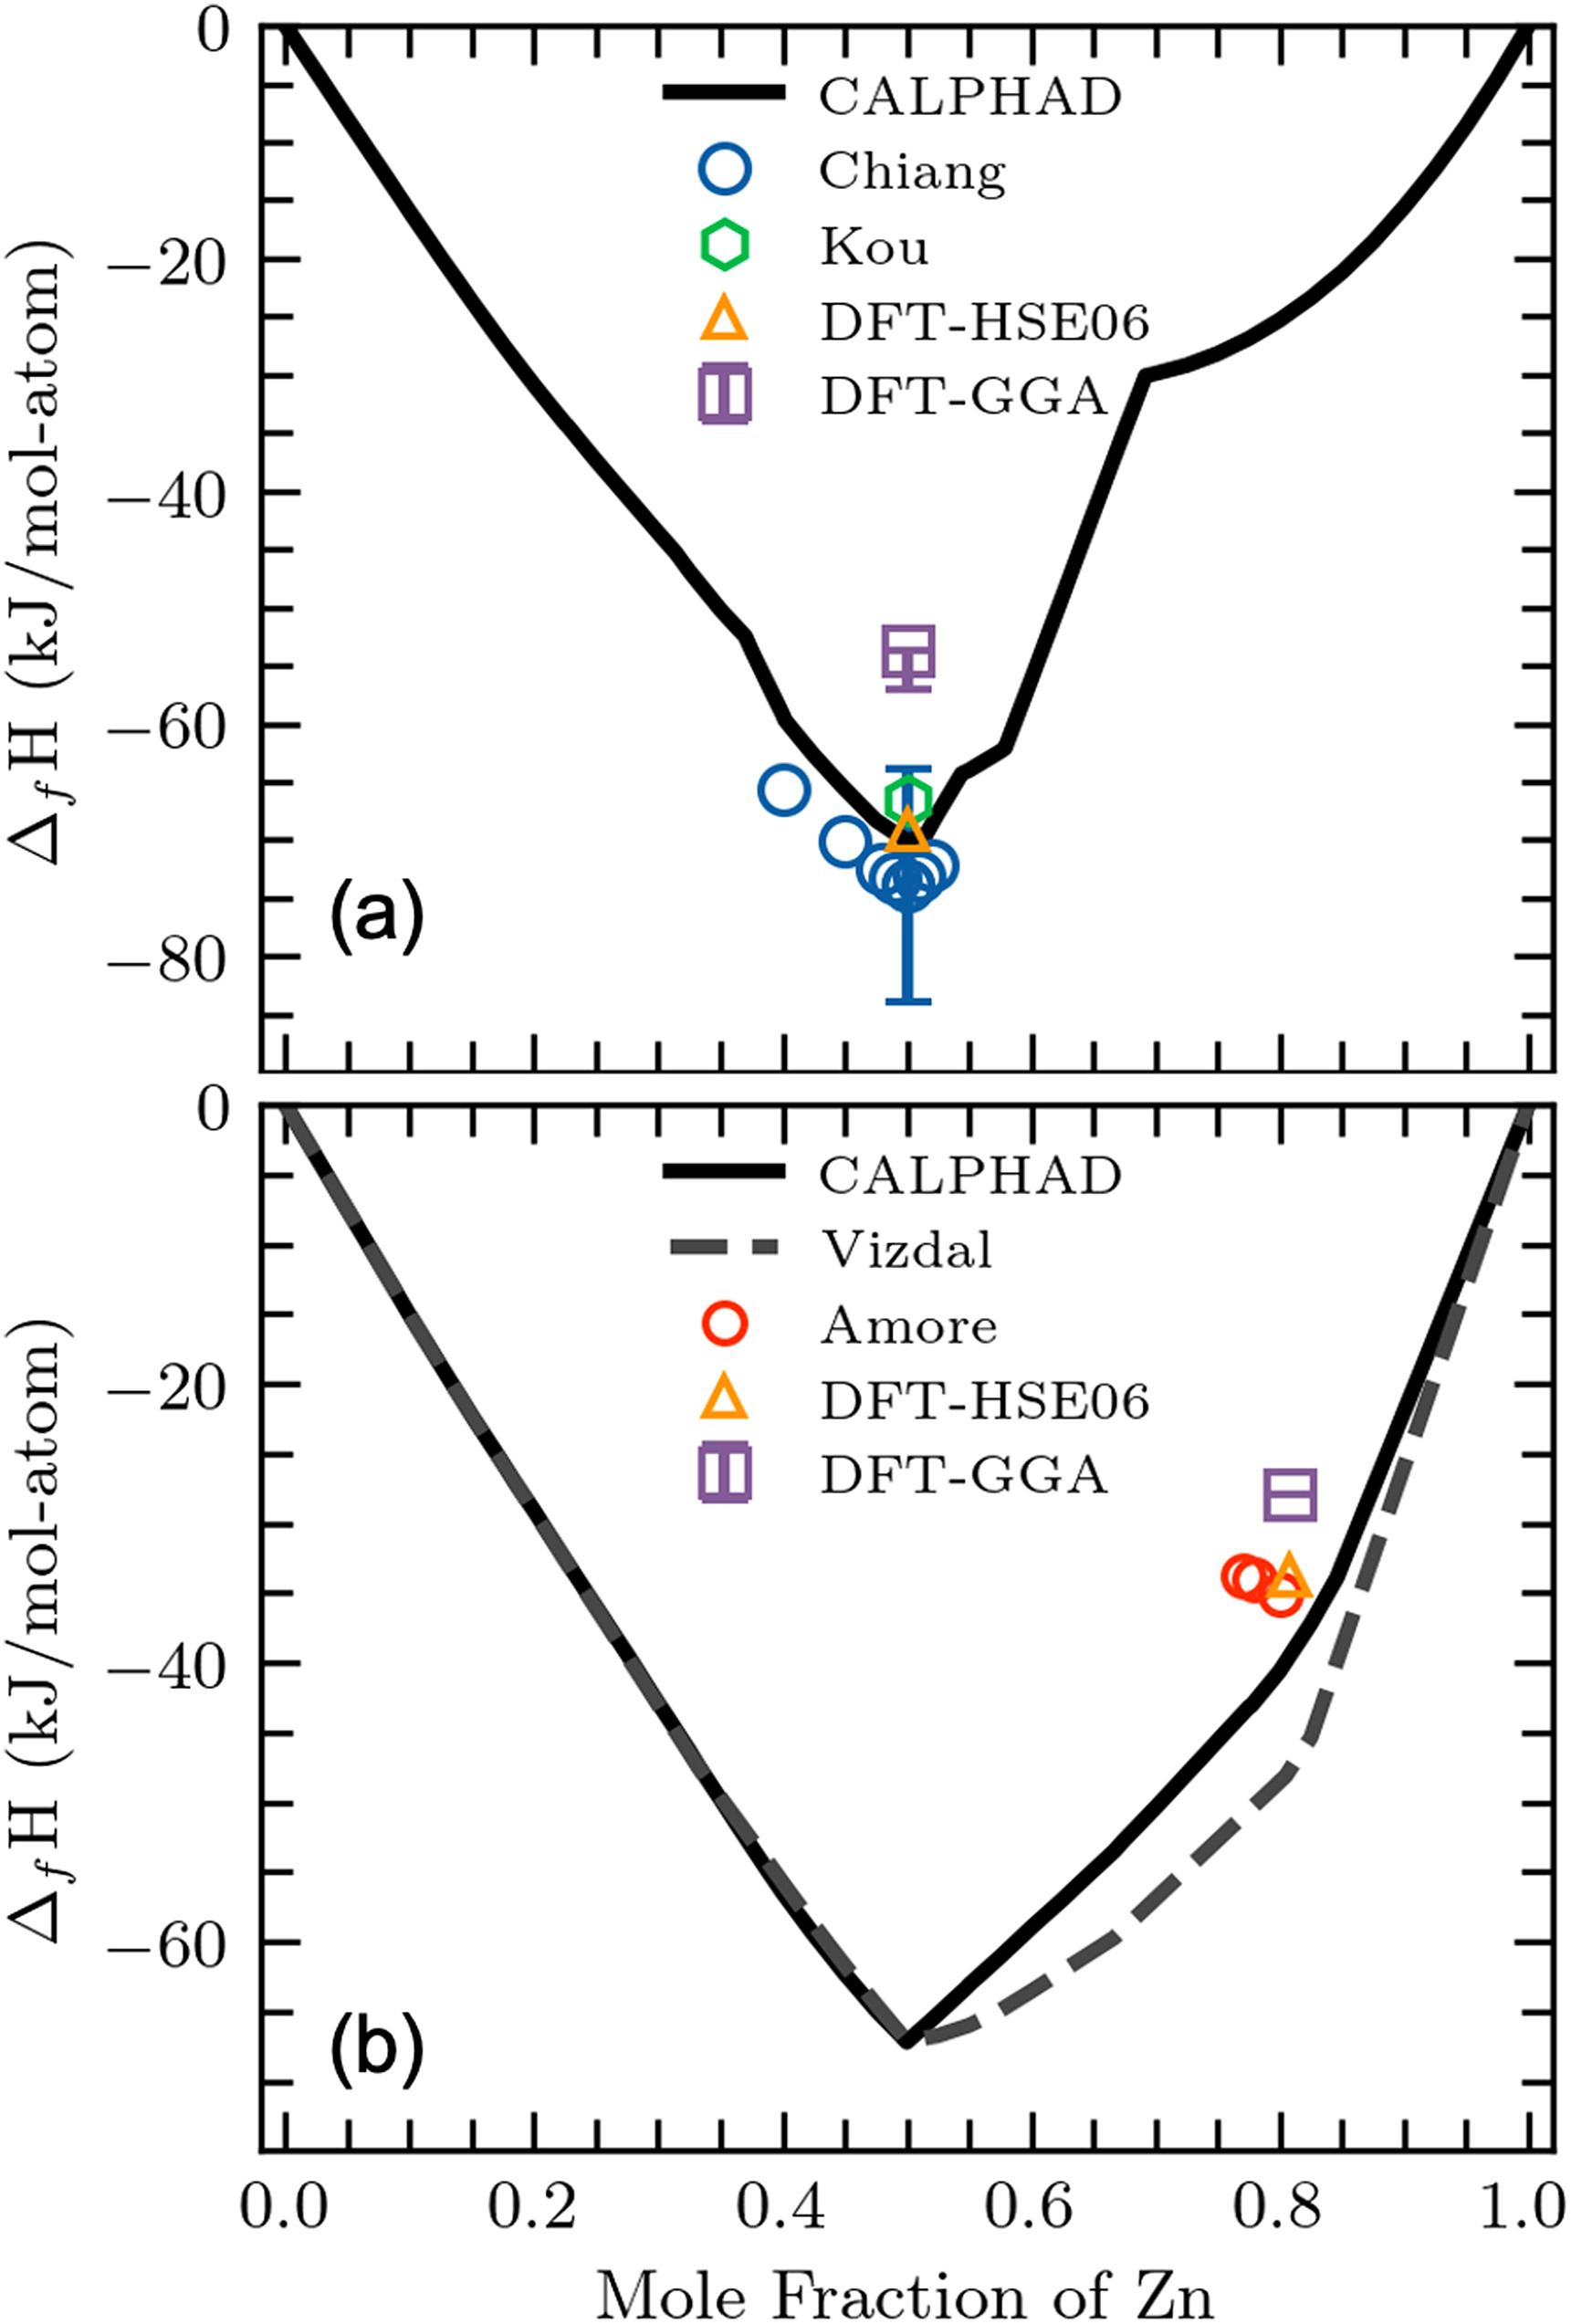
\includegraphics[width=0.5\linewidth]{intermetallics/Intermetallics-PdZnHMR.jpg}
    \caption{Calculated enthalpy of formation $\Delta_f$H at (a) 1273 K and (b) 300 K, along with DFT-based calculations and available experimental data by Chiang et al. \cite{ChiangIpserChang1977}, Kou and Chang \cite{kou1975thermodynamics}, and Amore et al. \cite{amore2009thermochemistry}. DFT using HSE is calculated at 0 K. DFT using GGA is calculated at 0 K and high temperatures 300 K and 1270 K respectively, shown as purple bars in the figure.}
    \label{intermetallics:fig:PdZnHMR}
\end{figure}

\subsection{Site occupancy in the $\gamma$-brass phase and surface construction} \label{intermetallics:ssec:PdZnsite}
Figure \ref{intermetallics:fig:PdZnSOC} shows the calculated site fractions in $\gamma$-brass at 773 K and 1023 K from the present model in comparison with XRD results by Edström et al. \cite{strom1969x}, Gourdon et al. \cite{gourdon2006intergrowth} and Dasgupta et al. \cite{Dasgupta2022}. Temperature has little influence on the site fraction of the $\gamma$-brass phase. With increasing Pd content, Pd is predicted first to occupy the OT sublattice, and then the OH sublattice after the OT sublattice is fully occupied. The site fractions of Pd in the OH sublattice are in good agreement with experimental data. For example, at $x_{Pd}$ = 0.173, the calculated site fraction of Pd in the OH sublattice $y_{Pd}^{\rm OH}$ is 0.08, slightly higher than 0.07 measured by Dasgupta et al.\cite{Dasgupta2022} At $x_{Pd}$ = 0.181, 0.192, and 0.23, the calculated $y_{Pd}^{\rm OH}$ values are 0.118, 0.165, and 0.333, respectively, which agree well with experimental data with a mean absolute error (MAE) of 0.002. Vizdal et al.'s \cite{vizdal2006experimental} model could not predict site fractions in $\gamma$-brass due to the 2-sublattice model used.

\begin{figure}[H]
    \centering
    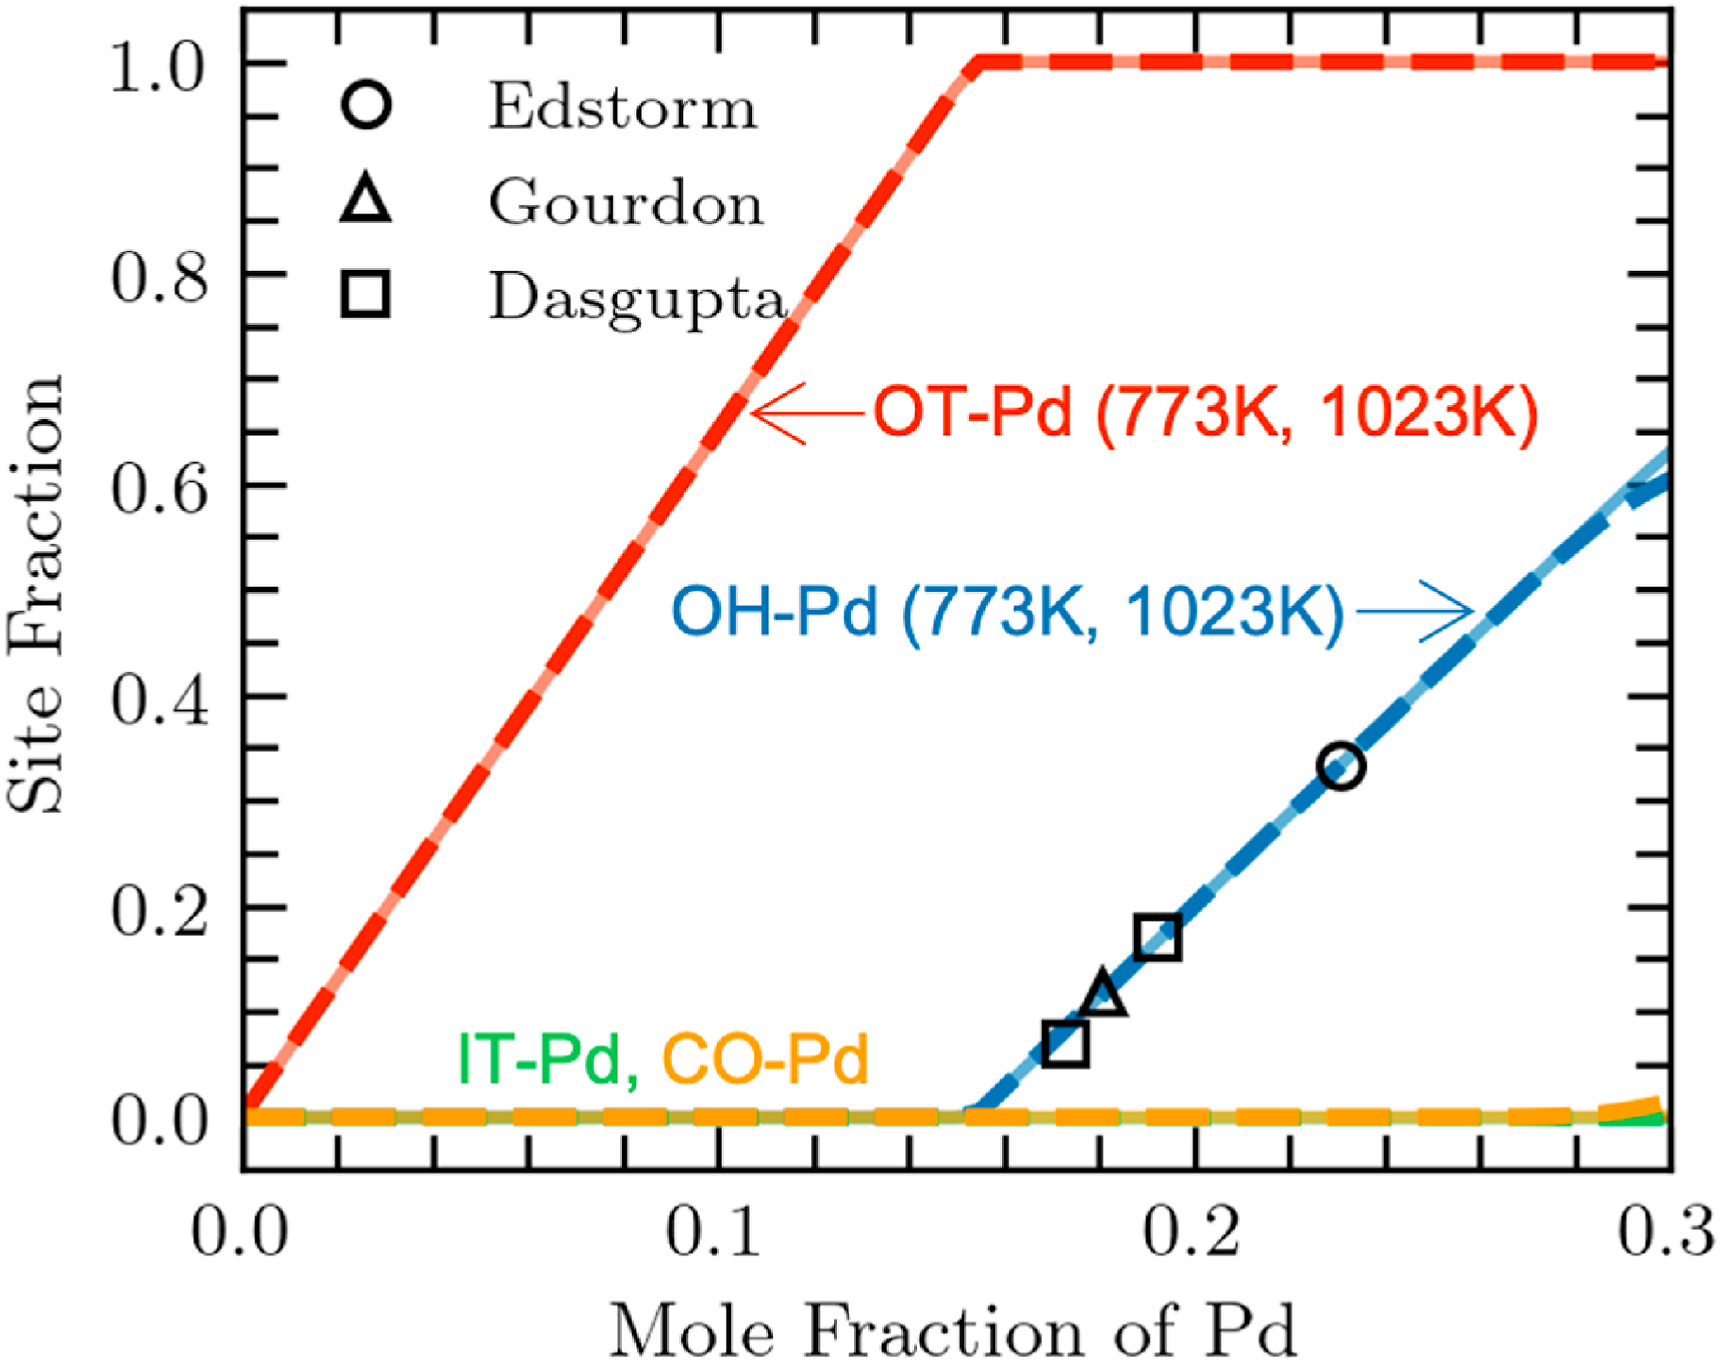
\includegraphics[width=0.5\linewidth]{intermetallics/Intermetallics-PdZnSOC.jpg}
    \caption{Calculated site fractions in $\gamma$-brass at 773K (solid lines) and 1023 K (dash lines) with the experimental data by Edström et al. \cite{strom1969x} at 923 K, Gourdon et al. \cite{gourdon2006intergrowth} at 1023 K, and Dasgupta et al. \cite{Dasgupta2022} at 773 K superimposed.}
    \label{intermetallics:fig:PdZnSOC}
\end{figure}

Force constants can be used to quantitatively understand interactions between atomic pairs \cite{shang2009first}. A large and positive force constant suggests a strong bonding interaction of an atomic pair, whereas a negative force constant indicates the tendency to separate \cite{yu2019synthesis}. To understand the site occupancy of Pd in $\gamma$-brass, we examined energies and force constants in three Pd$_9$Zn$_{43}$ configurations to analyze the occupancy of an additional Pd atom compared to the full Pd OT occupation in Pd$_8$Zn$_{44}$. Three configurations are $({{\rm Pd}_8)}^{\rm OH}{{(\rm Pd}_1{\rm Zn}_{11})}^{\rm OH}({{\rm Zn}_8)}^{\rm IT}({{\rm Zn}_{24})}^{\rm CO}$, \\$({{\rm Pd}_8)}^{\rm OH}{({\rm Zn}_{12})}^{\rm OH}({{{\rm Pd}_1\rm Zn}_7)}^{IT}({{\rm Zn}_{24})}^{\rm CO}$, and $({{\rm Pd}_8)}^{\rm OH}{({\rm Zn}_{12})}^{\rm OH}({{\rm Zn}_8)}^{IT}({{{\rm Pd}_1\rm Zn}_{23})}^{\rm CO}$, where 8 Pd atoms occupy 8 OT sites and the 9th Pd atom occupies one of the OH (conf\_OH), IT (conf\_IT), or CO (conf\_CO) sites, respectively. Force constants can be predicted by DFT-based phonon calculations \cite{shang2018understanding}. Table \ref{intermetallics:PdZn_DFT_details} lists details of phonon calculations for Pd$_9$Zn$_{43}$ configurations. Figure \ref{intermetallics:fig:PdZnFC} shows the force constants of atomic pairs Pd-Pd, Pd-Zn, and Zn-Zn in three Pd$_9$Zn$_{43}$ configurations. The Pd-Zn atomic pairs have the largest force constants 5.373 eV/\r{A}$^2$, compared with 4.875 eV/\r{A}$^2$ of Pd-Pd and 3.569 eV/\r{A}$^2$ of Zn-Zn pairs. It indicates that Pd-Zn pairs have the strongest bonding in the configuration. Table \ref{intermetallics:tab:PdZnfc} shows the energy and bonding in three Pd$_9$Zn$_{43}$ configurations, i.e., conf\_OH, conf\_IT, and conf\_CO. conf\_OH has the lowest energy $E_{conf\_OH}$ = -105.30 eV/atom and the shortest Pd-Zn bonding distance d$_{conf\_OH}^{Pd-Zn}$ = 2.538 \r{A} in comparison with conf\_CO and conf\_IT. In contrast, $d_{conf\_OH}^{Pd-Pd}$ = 2.940 \r{A} is larger than that of conf\_OH and conf\_IT. Table \ref{intermetallics:tab:PdZnfc} also shows the bonding of the 9th Pd when occupying OH, CO, and IT. In conf\_OH, the 9th Pd is bonding with Zn atoms in its first nearest neighbors ($d^{1NN}$ < 3.2 \r{A}, seen in Figure \ref{intermetallics:fig:PdZnFC}), with the nearest Pd atom is 4.713 \r{A} away. In conf\_CO and conf\_IT, there are Pd-Pd pairs in the first nearest neighbors of the 9th Pd, which makes the bonding between Pd and surroundings weaker than that in conf\_OH. We conclude that the stability preference for OH occupancy of additional Pd atoms results from stronger Pd-Zn bonding interactions.

\begin{figure}[H]
    \centering
    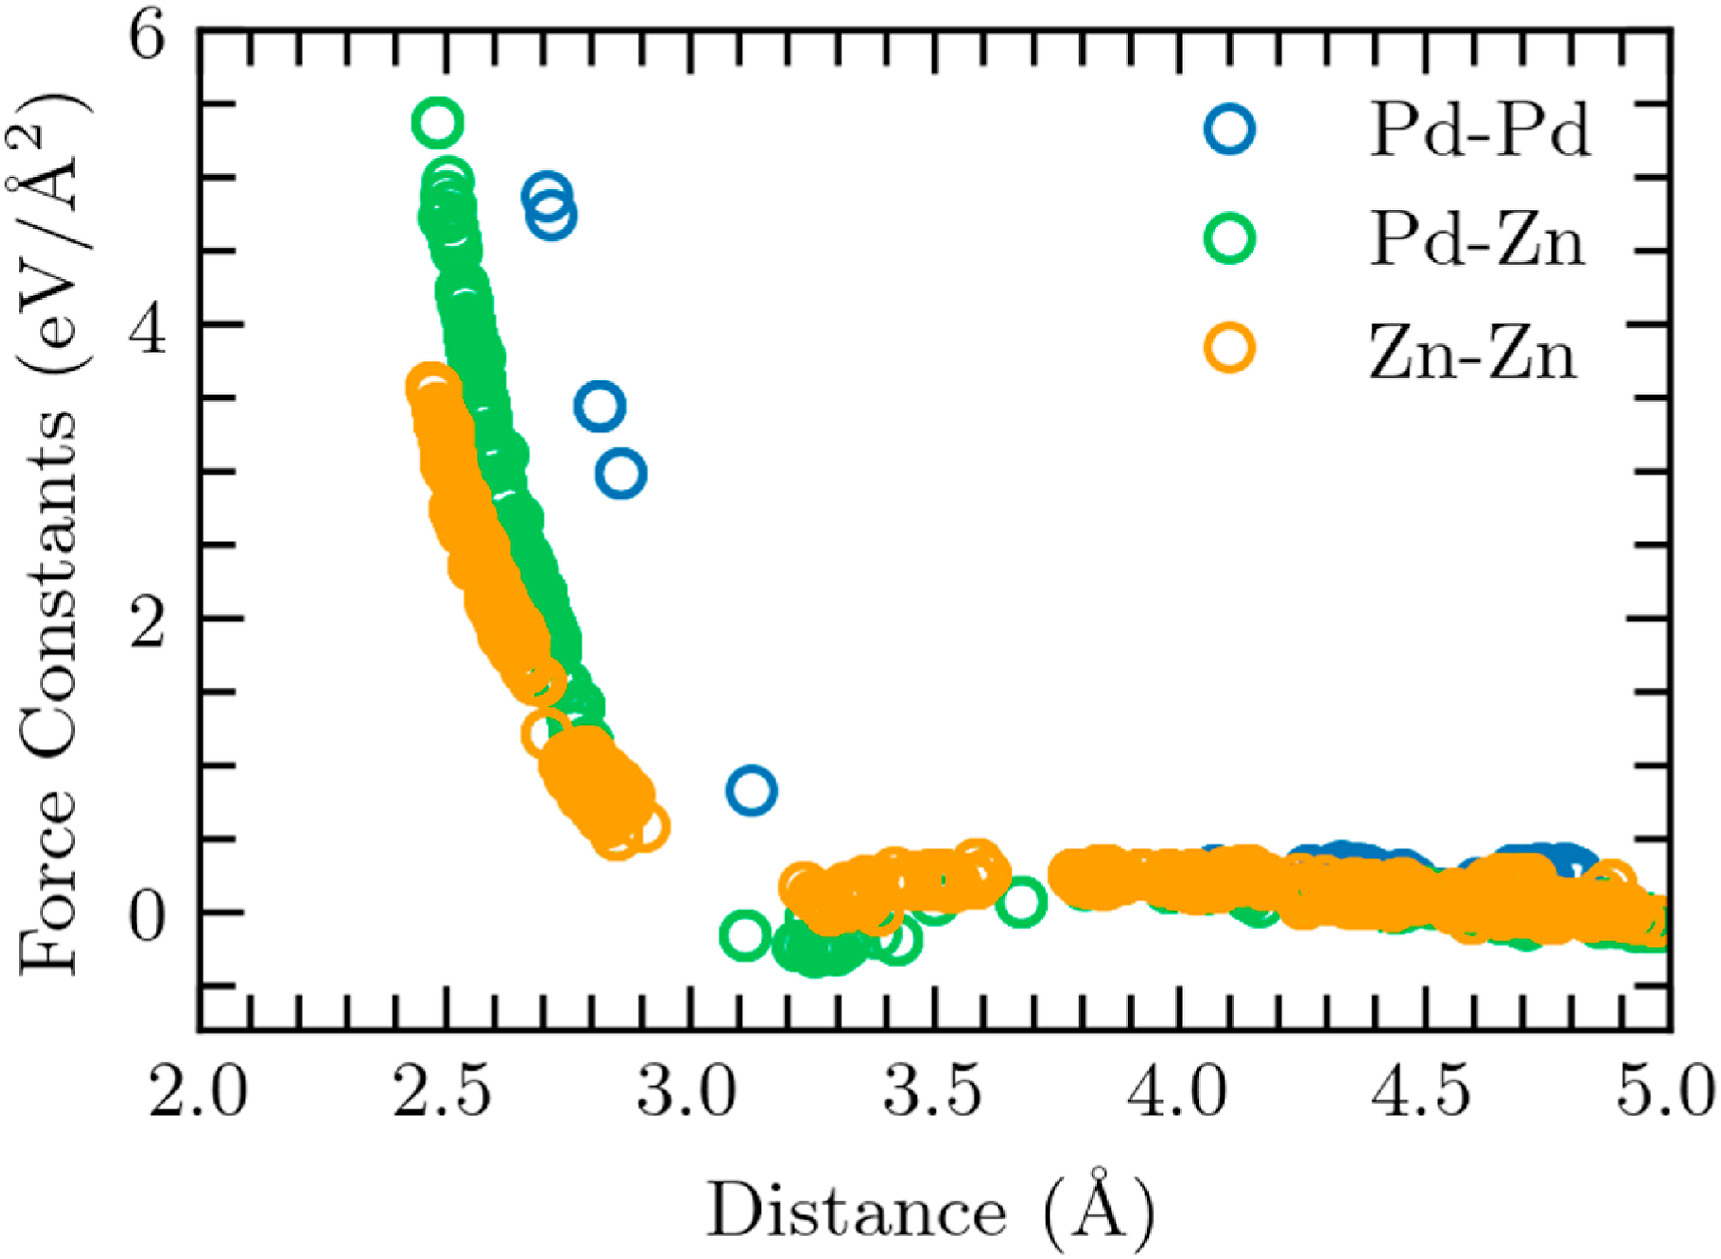
\includegraphics[width=0.5\linewidth]{intermetallics/Intermetallics-PdZnFC.jpg}
    \caption{Force constants of Pd-Pd, Pd-Zn, and Zn-Zn atom pairs in Pd$_9$Zn$_{43}$ configurations obtained from phonon calculations.}
    \label{intermetallics:fig:PdZnFC}
\end{figure}

\begin{table}[H]
    \centering
    \caption{Energies, and distances of bonds (d) of the nearest pairs for three Pd$_9$Zn$_{43}$ configurations with the first 8 Pd atoms occupying the OT site, and the 9th Pd atom (Pd$^{9th}$) occupying the OH, CO, or IT site, denoted by conf\_OH, conf\_CO, and conf\_IT, respectively. Configurations are relaxed using DFT calculations.}
    \begin{tabular}{>{\raggedright\arraybackslash}m{3cm}>{\raggedright\arraybackslash}m{3cm}>{\raggedright\arraybackslash}m{2cm}>{\raggedright\arraybackslash}m{2cm}>{\raggedright\arraybackslash}m{2.5cm}>{\raggedright\arraybackslash}m{2.5cm}}
        \hline
         \textbf{Configurations}& \textbf{Energy (eV/atom)} & d of Pd-Zn (\r{A}) & d of Pd-Pd (\r{A}) & d of Pd$^{9th}$-Zn (\r{A}) & d of Pd$^{9th}$-Pd (\r{A})\\
        \hline
        conf\_OH&-105.30&2.538&2.940&2.563&4.713\\
        conf\_CO&-104.89&2.558&2.783&2.562&2.783\\
        conf\_IT&-104.74&2.560&2.887&2.613&3.192\\
         \hline
    \end{tabular}
    \label{intermetallics:tab:PdZnfc}
\end{table}

Site fractions of $\gamma$-brass phase calculated from the CALPHAD modeling are further applied to analyze the surface structures. The possible stable composition of the $\gamma$-brass phase is evaluated ranging from Pd$_8$Zn$_{44}$ to Pd$_{12}$Zn$_{40}$ from the present model. It indicates that site occupancy in OH will be changed with changing Pd composition in the $\gamma$-brass phase, with OT remaining occupied by Pd, IT and CO occupied by Zn. DFT-based calculations have suggested that the $(1\bar{1}0)$ surface of the $\gamma$-brass phase has a lower surface energy than $(110)$ and ${111}$ \cite{Dasgupta2022}. Figure \ref{intermetallics:fig:PdZnSurface} shows $(1\bar{1}0)$ surface constructions of $\gamma$-brass phase. OT sites separately locate on the surface, forming Pd monomers (Pd1). When increase Pd occupy OH sites, OT-OH-OT ensembles on the surface can then become Pd trimers (Pd3). The ability to control the exposure of specific surface ensembles between Pd1 and Pd3 sites is a direct consequence of the site occupancies of the bulk structure and has catalytic consequences. For example, the activity for ethylene hydrogenation and selectivity for acetylene semi-hydrogenation were drastically altered by tuning active ensembles between Pd monomers (Pd1) and Pd trimers (Pd3) \cite{Dasgupta2022}. 

\begin{figure}[H]
    \centering
    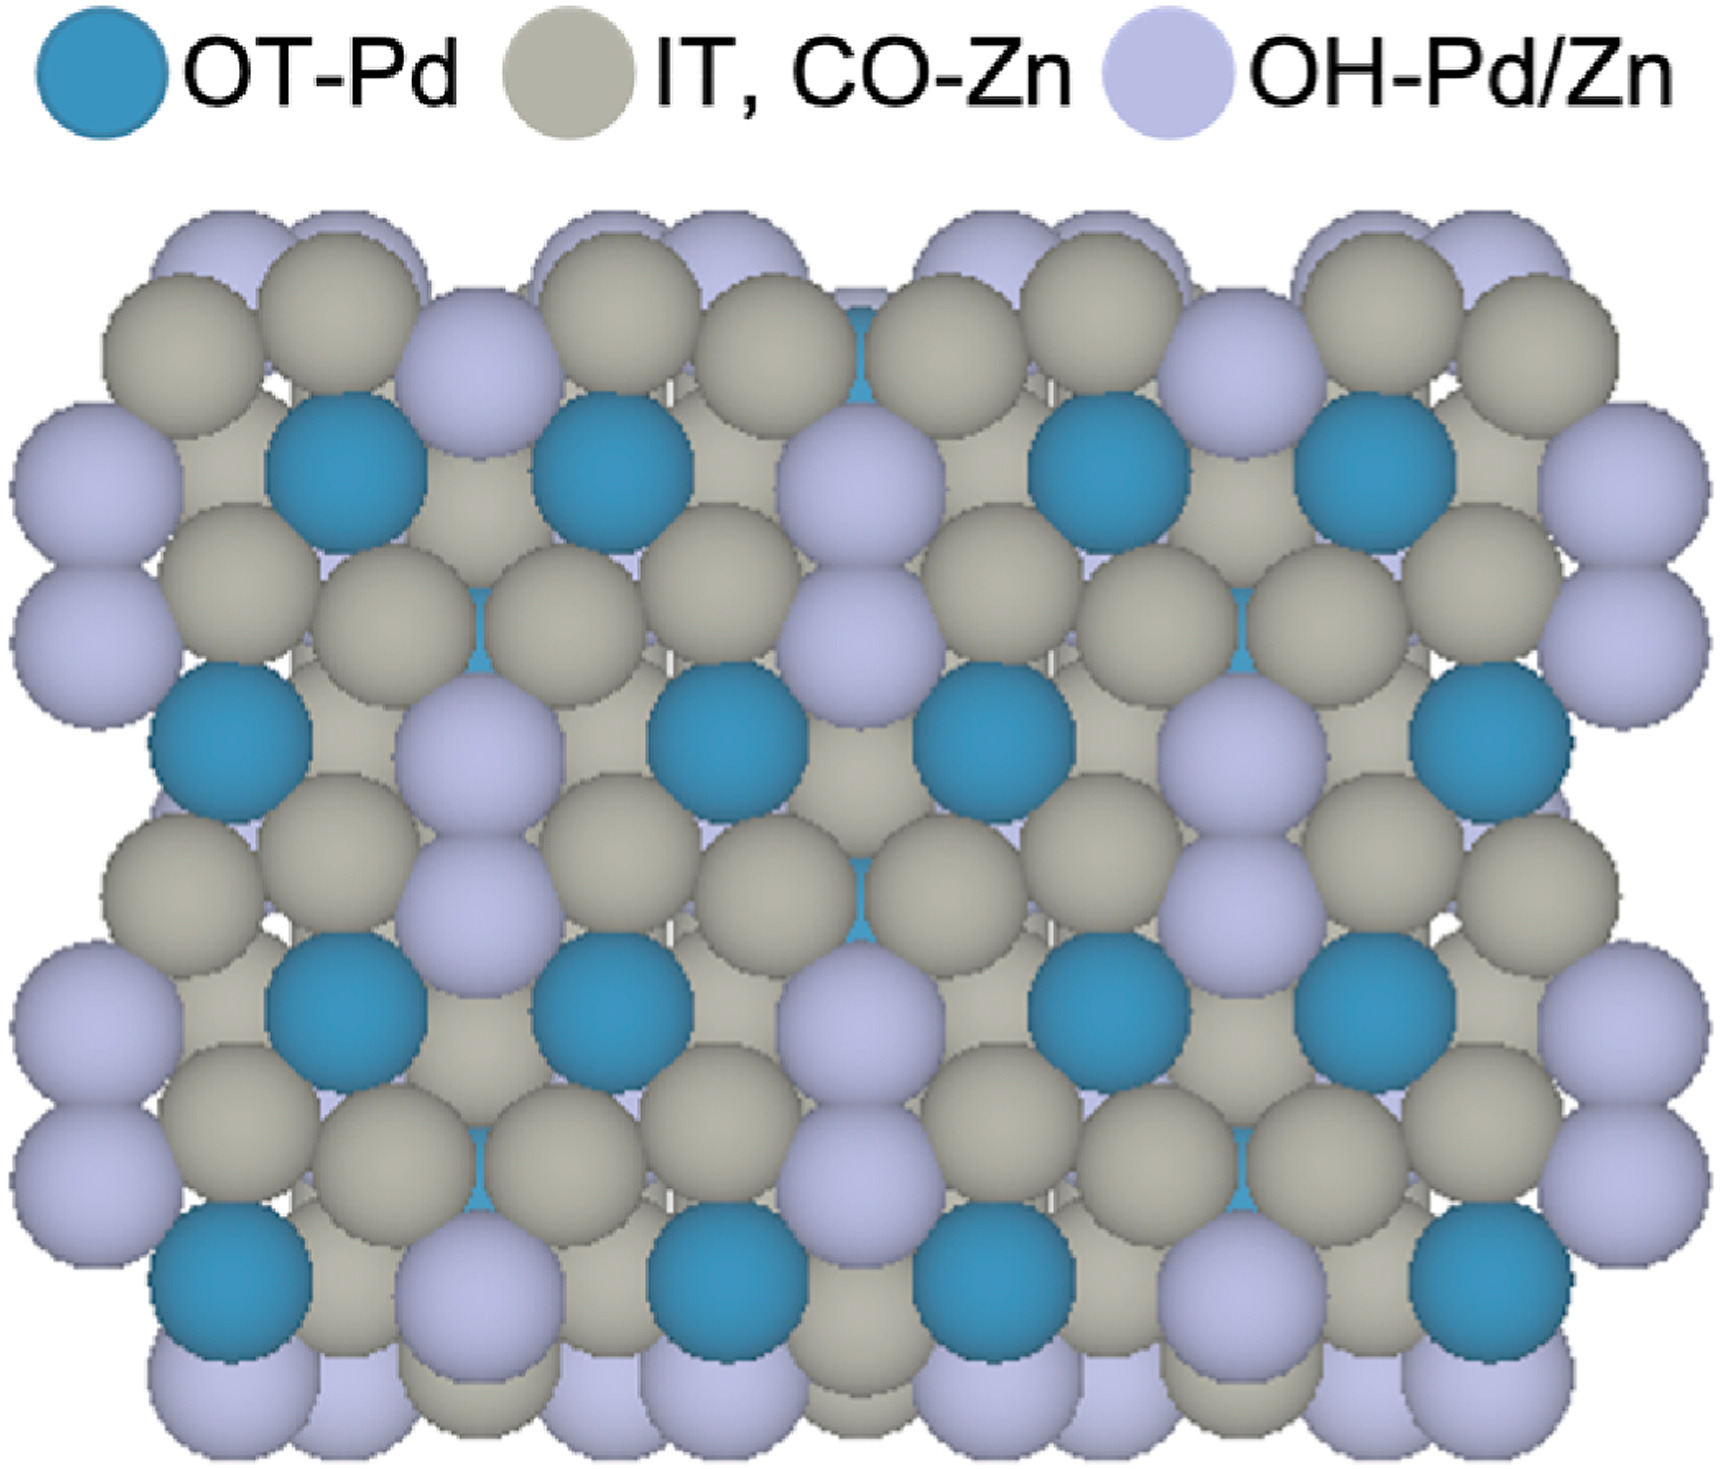
\includegraphics[width=0.4\linewidth]{intermetallics/Intermetallics-PdZnSurface.jpg}
    \caption{$(1\bar{1}0)$ surface of $\gamma$-brass in $2\times2\times2$ supercell. Blue atoms are OT sites, which are occupied by Pd atoms. Grey atoms are IT and CO sites, which are occupied by Zn atoms. Purple atoms are OH sites, which can be occupied by both Pd and Zn atoms.}
    \label{intermetallics:fig:PdZnSurface}
\end{figure}

\section{Determination of site occupancy in the M-Pd-Zn (M = Cu, Ag, and Au) \texorpdfstring{$\gamma$}--brass phase} \label{intermetallics:sec:PdZnM}
The Pd-Zn $\gamma$-brass phase provides exciting opportunities for synthesizing site-isolated catalysts with precisely controlled Pd active site ensembles. Introducing a third metal into the $\gamma$-brass lattice further perturbs the catalytic active site ensembles. Here, we introduce coinage metals M (M = Cu, Ag, and Au) into the Pd-Zn $\gamma$-brass phase and investigate the site occupation factors (SOF) of each element in the $\gamma$-brass lattice. The choice of M is motivated by the potential to synthesize new selective hydrogenation catalysts, as each of these metals have been previously utilized for catalyzing hydrogenation chemistries either as single metal catalysts \cite{chou1987benzene, chou1987benzeneII} or as Pd-M \cite{zhang2000synergetic, choudhary2003acetylene, chen2005promotional, friedrich2013order, mccue2014cu, kyriakou2012isolated} (or even M-Zn \cite{spanjers2014zinc}) bimetallic catalysts. The CALPHAD modeling approach and X-ray or neutron diffraction with Rietveld refinement were used to identify the SOF on each Wyckoff site for various M ratios alloyed into the Pd-Zn $\gamma$-brass phase. The present analysis unveils the strong preference for Pd occupying the OT site in the $\gamma$-brass lattice while the coinage metals tend to substitute for Zn on the OH site.  The determination of site occupancy in the bulk M-Pd-Zn $\gamma$-brass phase provides opportunities to investigate possible catalytic active site ensembles in the $\gamma$-brass phase materials.

\subsection{Modeling details} \label{intermetallics:ssec:PdZnMmodel}
The model of the M-Pd-Zn $\gamma$-brass phase is based on the compound energy formalism according to its Wyckoff sites (see Section \ref{method:ssec:CEF}). To this end, a four-sublattice model has been used:
\begin{equation} \label{intermetallics:eq:PdZnMmodel}
    \mathrm{(Pd,Zn,M)_2(Pd,Zn,M)_3(Pd,Zn,M)_2(Pd,Zn,M)_6}
\end{equation}
to describe the $\gamma$-brass phase, corresponding to the OT, OH, IT, and CO sites of space group $I\overline{4}3m$, respectively \cite{strom1969x}. The Gibbs energy expression for this $\gamma$-brass phase modeled using four sublattices is:
\begin{equation}
    \begin{aligned}
        G_m=&\sum_{i={\rm Pd,Zn,M}}\sum_{j={\rm Pd,Zn,M}}\sum_{k={\rm Pd,Zn,M}}\sum_{l={\rm Pd,Zn,M}}{y_i^\prime y_j^{\prime\prime}y_k^{\prime\prime\prime}y_l^{\prime\prime\prime\prime}{{^o}G}_{i:j:k:l}}\\&+RT(2\sum_{i={\rm Pd,Zn,M}}{y_i^\prime\ln{\left(y_i^\prime\right)}+}3\sum_{j={\rm Pd,Zn,M}}{y_j^{\prime\prime}\ln{\left(y_j^{\prime\prime}\right)}}\\&+2\sum_{k={\rm Pd,Zn,M}}{y_k^{\prime\prime\prime}\ln{\left(y_k^{\prime\prime\prime}\right)}+}6\sum_{l={\rm Pd,Zn,M}}{y_l^{\prime\prime\prime\prime}\ln{\left(y_l^{\prime\prime\prime\prime}\right)}})+{^{xs}}G_m
    \end{aligned}
\end{equation}
where $y_i^{\left(s\right)}$ is the site fraction of component $i$ on sublattice $s$ with $s$ = $\prime$, $\prime\prime$, $\prime\prime\prime$, and $\prime\prime\prime\prime$, representing the OT, OH, IT, and CO sublattice, respectively. ${^o}G_{i:j:k:l}$ is the energy of the endmember $\left(i\right)_2\left(j\right)_3\left(k\right)_2\left(l\right)_6$ with only one component ($i$, $j$, $k$, or $l$) in each sublattice.The second to the fifth terms represent the configurational entropy contribution to Gibbs energy, and $^{xs}G_m$ is the excess Gibbs energy. For simplicity, the effects of $^{xs}G_m$ are ignored, given the complexity of describing the Gibbs energy with the four-sublattice model and the numerous terms involved.

The thermodynamic model of the $\gamma$-brass phase in Pd-M-Zn was established using the open-source software ESPEI \cite{bocklund2019espei}. The parameters in the model were generated using thermochemical data from DFT-based first-principles calculations as discussed in the following paragraphs, and the Gibbs energies of pure elements (Pd, Zn, Cu, Ag, and Au) were taken from the Scientific Group Thermodata Europe (SGTE) database \cite{sgteurl}.

DFT-based first-principles calculations in the present work were performed to predict the energetics of the endmembers for the M-Pd-Zn $\gamma$-brass phase. The static total energy, $E\left(V\right)$, of a given endmember at 0 K is obtained as a function of volume ($V$), fitted using a four-parameter Birch-Murnaghan equation of state as shown in (\ref{method:eq:EOS}). The VASP package \cite{kresse1996efficient} was employed for all DFT calculations. The projector augmented-wave method (PAW) was used to account for the electron-ion interactions in order to increase computational efficiency in comparison with the full potential methods \cite{blochl1994projector}. Electron exchange and correlation effects were described using the generalized gradient approximation (GGA) as implemented by Perdew, Burke, and Ernzerhof (PBE) \cite{perdew1996generalized}. In the present work, 81 endmembers using a 26-atom cell in each of the M-Pd-Zn systems (M = Cu, Ag, and Au) were calculated. For each endmember, DFT calculations were performed using 8 volumes for the energy versus volume (E-V) EOS fitting with $V/V_0$ in the range of 0.91 $-$ 1.12. The k-points meshes were $7\times7\times7$ for structure relaxations and static calculations. The plane-wave basis cutoff energy was set as accurate (i.e., the setting of “PREC = Accurate” for VASP) for relaxations and 520 eV for the final static calculations. The convergence criterion of the electronic self-consistency was set as 5×10$^{-6}$ eV/atom for relaxations and final calculations.

\subsection{Properties of M-Pd-Zn (M = Cu, Ag, and Au) $\gamma$-brass compounds by first-principles calculations} \label{intermetallics:ssec:PdZnMDFTresult}
Figure \ref{intermetallics:fig:PdZnM-ConvexHull} shows the convex hull of formation enthalpy in the Cu-Pd-Zn, Ag-Pd-Zn, and Au-Pd-Zn $\gamma$-brass phase. Figure \ref{intermetallics:fig:PdZnM-ConvexHull} only displays endmembers within the $\gamma$-brass phase, disregarding other phases that may be present in the ternary system. Six ternary endmembers are identified on the convex hull in the Au-Pd-Zn $\gamma$-brass phase, i.e., $\mathrm{\left(Au\right)_4^{OT}\left(Zn\right)_6^{OH}\left(Pd\right)_4^{IT}\left(Au\right)_{12}^{CO}}$, $\mathrm{\left(Pd\right)_4^{OT}\left(Au\right)_6^{OH}\left(Zn\right)_4^{IT}\left(Zn\right)_{12}^{CO}}$, $\mathrm{\left(Pd\right)_4^{OT}\left(Pd\right)_6^{OH}\left(Zn\right)_4^{IT}\left(Au\right)_{12}^{CO}}$, $\mathrm{\left(Pd\right)_4^{OT}\left(Zn\right)_6^{OH}\left(Au\right)_4^{IT}\left(Pd\right)_{12}^{CO}}$, \\$\mathrm{\left(Zn\right)_4^{OT}\left(Pd\right)_6^{OH}\left(Zn\right)_4^{IT}\left(Au\right)_{12}^{CO}}$, and $\mathrm{\left(Zn\right)_4^{OT}\left(Zn\right)_6^{OH}\left(Pd\right)_4^{IT}\left(Au\right)_{12}^{CO}}$. In the Cu-Pd-Zn $\gamma$-brass phase, two ternary endmembers lie on the convex hull, including $\mathrm{\left(Cu\right)_4^{OT}\left(Zn\right)_6^{OH}\left(Zn\right)_4\left(Pd\right)_{12}^{CO}}$ in the Pd rich region and $\mathrm{\left(Pd\right)_4^{OT}\left(Cu\right)_6^{OH}\left(Zn\right)_4^{IT}\left(Zn\right)_{12}^{CO}}$ in the Zn rich region. For the Ag-Pd-Zn system, only $\mathrm{\left(Pd\right)_4^{OT}\left(Ag\right)_6^{OH}\left(Zn\right)_4^{IT}\left(Zn\right)_{12}^{CO}}$ is on the convex hull within the ternary composition region. Notably, $\mathrm{\left(Pd\right)_4^{OT}\left(M\right)_6^{OH}\left(Zn\right)_4^{IT}\left(Zn\right)_{12}^{CO}}$ (M=Cu, Ag, and Au) are on the convex hull in all three systems, indicating Pd prefers the OT site while the coinage metals M prefer the OH site in the $\gamma$-brass phase. 

\begin{figure}[H]
    \centering
    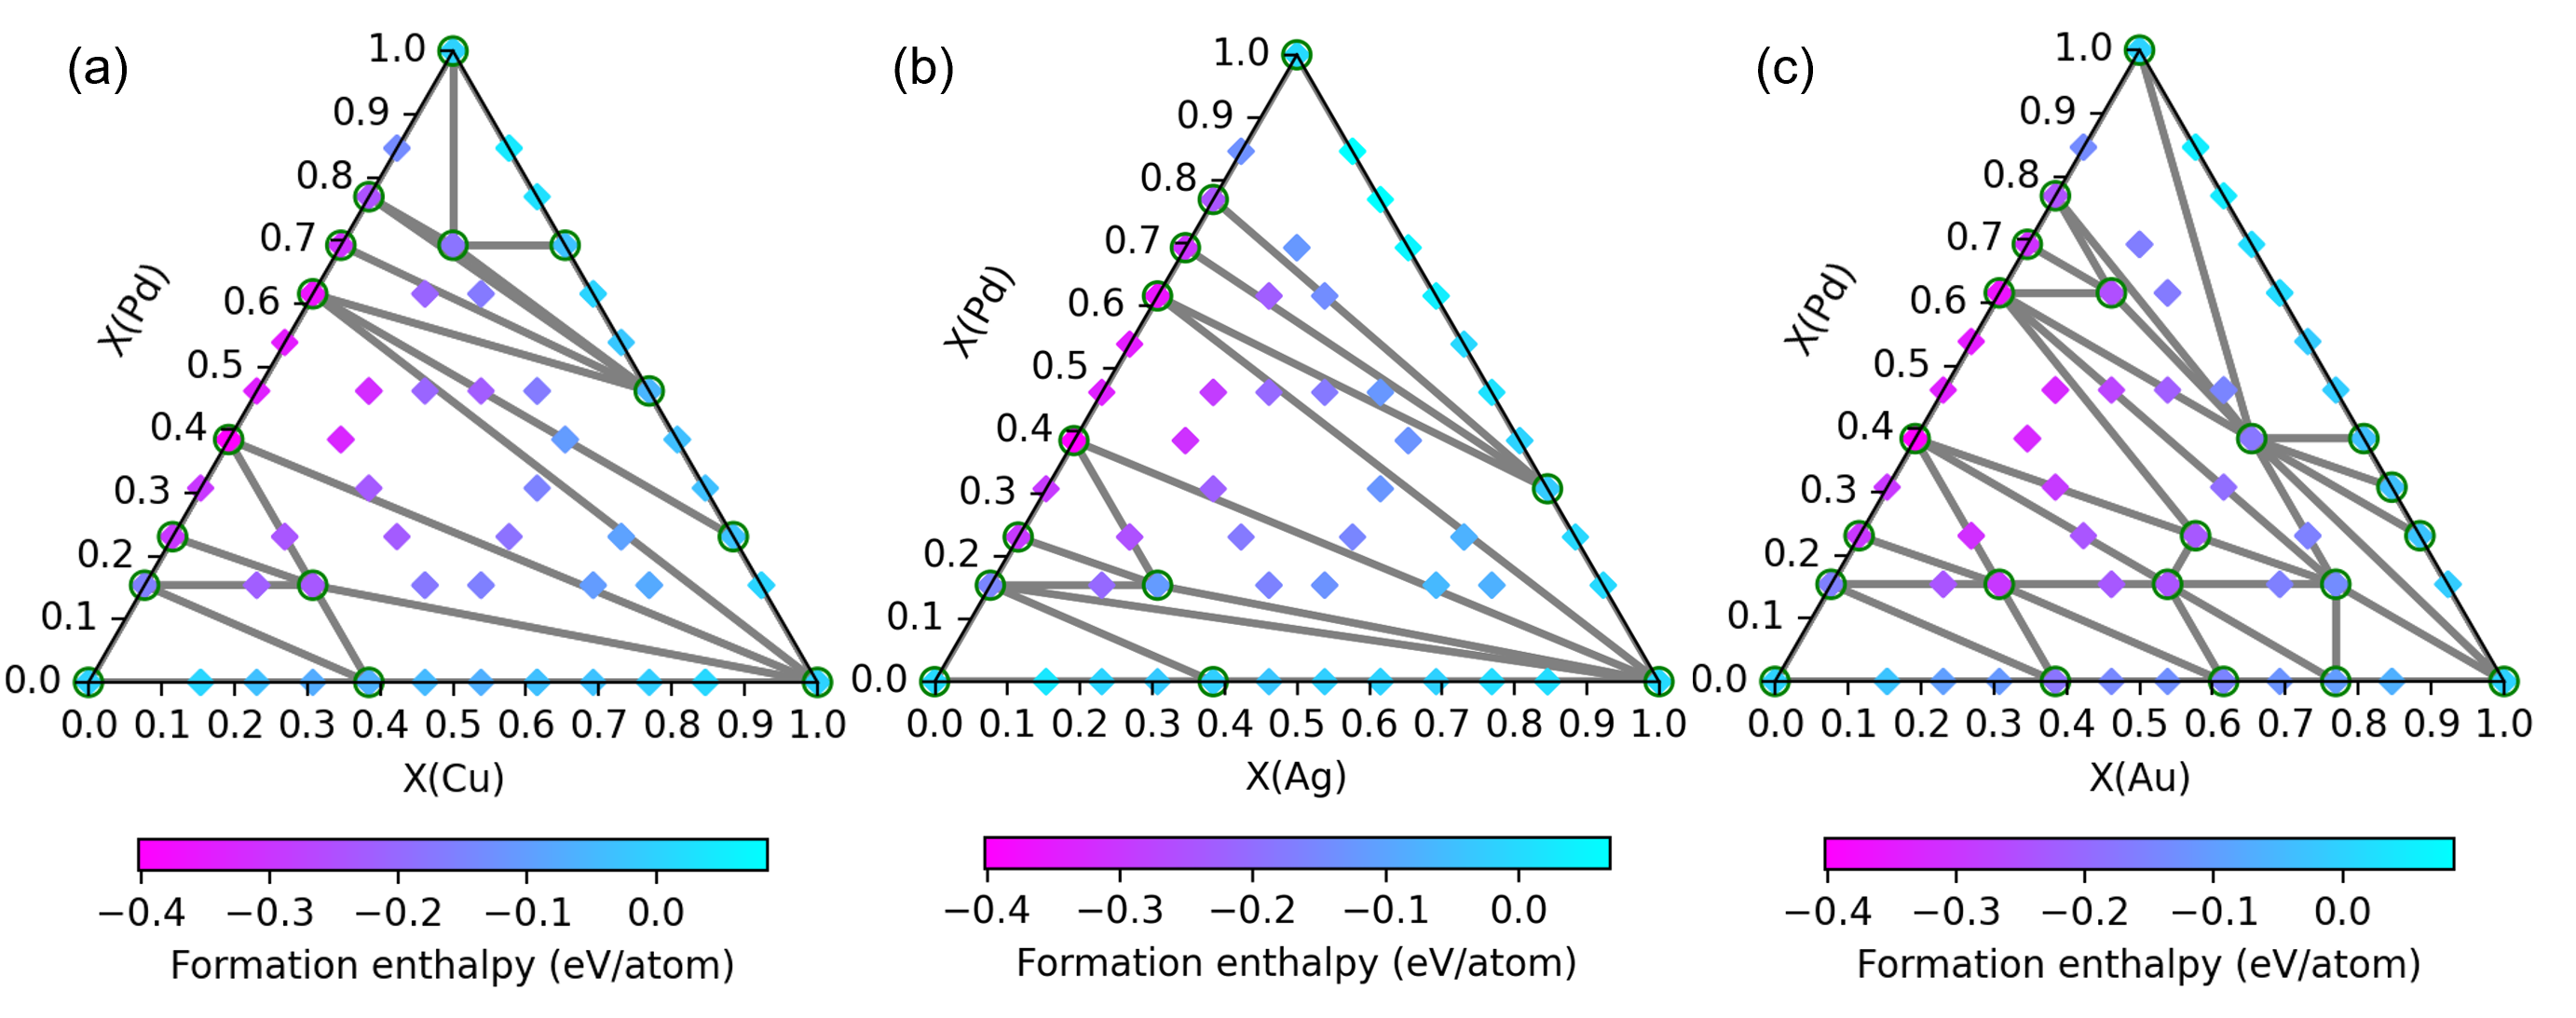
\includegraphics[width=1.0\linewidth]{intermetallics/Intermetallics-PdZnM-ConvexHull.png}
    \caption{Convex hull at 0 K in (a) Cu-Pd-Zn, (b) Ag-Pd-Zn, and (c) Au-Pd-Zn $\gamma$-brass phases. Green circles represent compounds on the convex hull. Diamonds represent compounds above the hull, with more purple showing lower formation enthalpy and more blue showing higher formation enthalpy. The reference states used for calculations are FCC Cu, Ag, Au, Pd, and HCP Zn.}
    \label{intermetallics:fig:PdZnM-ConvexHull}
\end{figure}

The convex hull facet shape near the Zn rich corner (x(Zn) > 0.6) should be emphasized, especially considering the appearance of the $\gamma$-brass phase in the Zn rich region in the binary phases diagrams (x(Zn) = 0.77 ~ 0.85 in the Pd-Zn system7, x(Zn) around 0.6 in the Ag-Zn system, and x(Zn) = 0.65~0.75 in the Au-Zn system66). Considering x(Zn) > 0.6 and x(Pd) < 0.15 in Figure 1, the convex hull facet shape in the Ag-Pd-Zn $\gamma$-brass phase differs from the Cu-Pd-Zn and Au-Pd-Zn $\gamma$-brass phases. In the Cu-Pd-Zn and Au-Pd-Zn $\gamma$-brass phases, the convex hull facet consists of $\mathrm{\left(Pd\right)_4^{OT}\left(Zn\right)_6^{OH}\left(Zn\right)_4^{IT}\left(Zn\right)_{12}^{CO}}$, $\mathrm{\left(Pd\right)_4^{OT}\left(M\right)_6^{OH}\left(Zn\right)_4^{IT}\left(Zn\right)_{12}^{CO}}$, and $\mathrm{\left(M\right)_4^{OT}\left(M\right)_6^{OH}\left(Zn\right)_4^{IT}\left(Zn\right)_{12}^{CO}}$. However, in the Ag-Pd-Zn $\gamma$-brass phase, one facet is composed of $\mathrm{\left(Pd\right)_4^{OT}\left(Zn\right)_6^{OH}\left(Zn\right)_4^{IT}\left(Zn\right)_{12}^{CO}}$, $\mathrm{\left(Pd\right)_4^{OT}\left(Ag\right)_6^{OH}\left(Zn\right)_4^{IT}\left(Zn\right)_{12}^{CO}}$, and pure Ag. The other consists of $\mathrm{\left(Pd\right)_4^{OT}\left(Zn\right)_6^{OH}\left(Zn\right)_4^{IT}\left(Zn\right)_{12}^{CO}}$, $\mathrm{\left(Ag\right)_4^{OT}\left(Ag\right)_6^{OH}\left(Zn\right)_4^{IT}\left(Zn\right)_{12}^{CO}}$, and pure Ag. In Ag-Pd-Zn, the endmembers on the convex hull are notably affected by the Pd ratio in the $\gamma$-brass phase. With decreasing Pd composition, the ternary endmember $\mathrm{\left(Pd\right)_4^{OT}\left(Ag\right)_6^{OH}\left(Zn\right)_4^{IT}\left(Zn\right)_{12}^{CO}}$ disappears from the convex hull. The solubility range of a homogeneous ternary $\gamma$-brass phase in the Ag-Pd-Zn system is narrower, and its stability is more sensitive to Pd composition than the Cu-Pd-Zn and Au-Pd-Zn systems. It is consistent with the experimental observation from the collaborators that the lower Pd composition, due to the increased Ag content, causes the decomposition of the homogeneous Ag-Pd-Zn ternary $\gamma$-brass into Ag-Zn $\gamma$-brass and Pd-Zn $\gamma$-brass phases.   

\subsection{Site occupancy predicted by CALPHAD modeling approach and compared with experiments} \label{intermetallics:ssec:PdZnMCALPHADresult}
The site fraction of each element in each sublattice can be calculated using the CALPHAD modeling approach under given conditions such as the fixed temperature $T$, pressure $P$, and mole fraction of Pd, i.e., $x$(Pd). We consider the conditions of $T$ = 300 K, $P$ =101325 Pa, and $x$(Pd) = 0.1538 (8 Pd atoms in a 52-atom supercell) to predict the site fractions of alloying elements M on each sublattice (OT, OH, IT, and CO). The selected composition x(Pd) = 0.1538 is consistent with the low $x$(Pd) limit evaluated from thermodynamic modeling of the Pd-Zn system for formation of a stable Pd-Zn $\gamma$-brass system \cite{gong2022thermodynamic}. Figure \ref{intermetallics:fig:PdZnM-SiteFractionCalphad} shows the predicted site occupancies of the alloying elements M (= Cu, Ag, and Au), Pd, and Zn as a function of the mole fraction of M, i.e., $x$(M). Figure \ref{intermetallics:fig:PdZnM-SiteFractionCalphad} plots the composition range of $x$(M) = 0 $-$ 0.1 (Pd$_8$M$_0$Zn$_{44}$ to around Pd$_8$M$_5$Zn$_{39}$) for dilute alloying elements. Figure \ref{intermetallics:fig:PdZnM-SiteFractionCalphad} shows the same trend of site occupancy in the three M-Pd-Zn (M=Cu, Ag, and Au) $\gamma$-brass phases. The site fraction of M on the OH sublattice increases with increasing $x$(M) in this composition range. The OT sites are fully occupied by Pd initially and remain unchanged when alloying $x$(M) into the $\gamma$-brass phase. The site fraction of Zn on the OH site decreases when increasing $x$(M). 

Table \ref{intermallics:tab:SFPdMZn} shows the detailed site fraction values at the composition of Pd$_8$M$_1$Zn$_{43}$ calculated by the CALPHAD approach. This composition is chosen to unveil the site preference of one M atom alloyed with the Pd-Zn $\gamma$-brass phase (Pd$_8$Zn$_{44}$) \cite{gong2022thermodynamic}. In all M-Pd-Zn (M=Cu, Ag, and Au) $\gamma$-brass phases, the site fraction $y_{\rm M}^{\rm OH}$ is around 0.08. In addition, there is a small amount of M entering the IT and CO sites, for example, $y_{\rm Ag}^{\rm IT}$=0.0015 and $y_{\rm Ag}^{\rm CO}$=0.0010. However, $y_{\rm Pd}^{\rm OT}$ remains at 1 in all three M-Pd-Zn $\gamma$-brass phases when adding M, indicating Pd atoms strongly outcompete M for the OT site. Overall, CALPHAD modeling predicts coinage M atoms prefer substituting Zn on the OH site when alloyed into the Pd-Zn $\gamma$-brass phase. 

\begin{figure}[H]
    \centering
    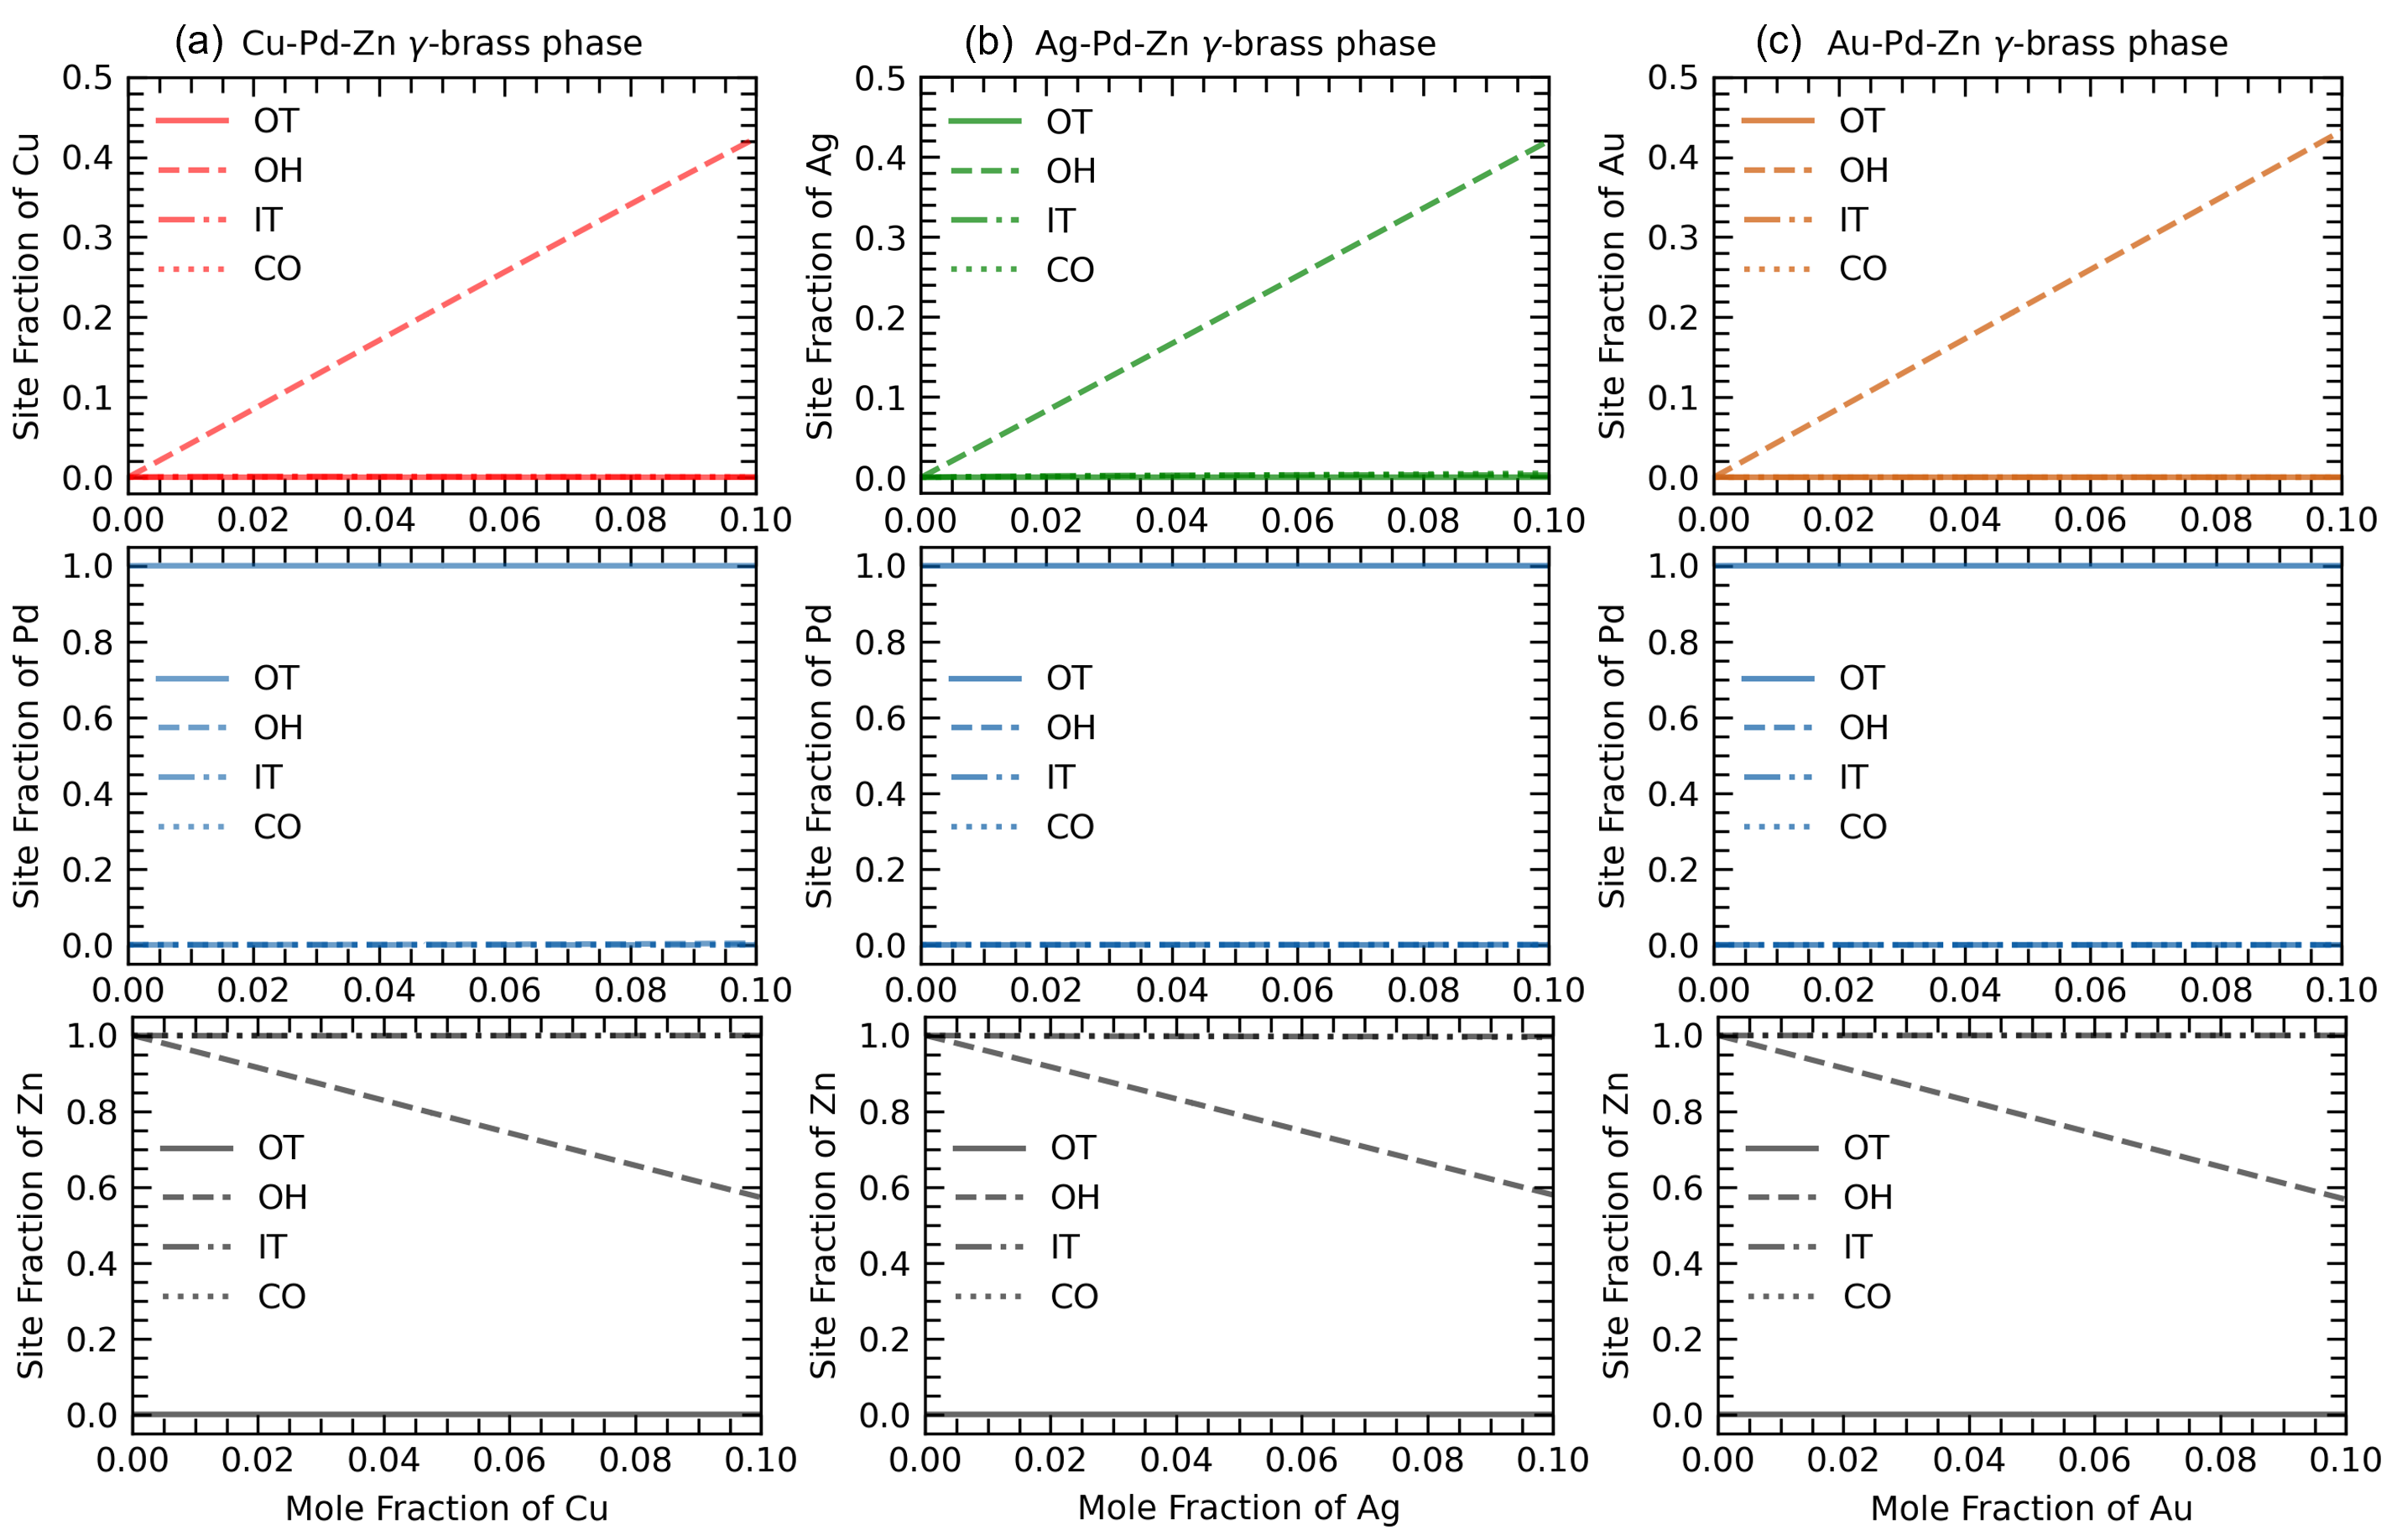
\includegraphics[width=1\linewidth]{intermetallics/Intermetallics-PdZnM-SiteFractionCalphad.png}
    \caption{Site fraction of each element in the (a) Cu-Pd-Zn, (b) Ag-Pd-Zn, and (c) Au-Pd-Zn $\gamma$-brass phases in OT (solid lines), OH (dashed lines), IT (dot-dashed lines), and CO (dotted lines) sublattice changing with increasing $x$(M) calculated from the CALPHAD modeling at T=300K, P=101325 Pa, and $x$(Pd)=0.1538. Red lines represent the site fraction of Cu, green lines represent the site fraction of Ag, orange lines represent the site fraction of Au, blue lines represent the site fraction of Pd, and grey lines represent the site fraction of Zn.}
    \label{intermetallics:fig:PdZnM-SiteFractionCalphad}
\end{figure}

\begin{table}[H]
    \centering
    \caption{Site fractions $y$ of Pd, Zn, and M (M= Cu, Ag, and Au) in each sublattice, denoted as $y_i^{\rm OT}$, $y_i^{\rm OH}$, $y_i^{\rm IT}$, and $y_i^{\rm CO}$, in ternary M-Pd-Zn $\gamma$-brass phases calculated from the CALPHAD modeling at temperature of 300 K, $x$(Pd)=0.1538, $x$(M)=0.0192 (Pd$_8$M$_1$Zn$_{43}$).}
    \begin{tabular}{>{\raggedright\arraybackslash}m{3cm}>{\raggedright\arraybackslash}m{2.5cm}>{\raggedright\arraybackslash}m{2cm}>{\raggedright\arraybackslash}m{2cm}>{\raggedright\arraybackslash}m{2cm}>{\raggedright\arraybackslash}m{2cm}}
        \hline
        \textbf{Composition}&\textbf{Element $i$}&$y_i^{\rm OT}$&$y_i^{\rm OH}$&$y_i^{\rm IT}$&$y_i^{\rm CO}$\\
        \hline
        Pd$_8$Cu$_1$Zn$_{43}$&Cu&0.000&0.082&0.001&0.000\\
	&Pd&1.000&0.0000&0.0000&0.000\\
	&Zn&0.000&0.918&0.999&1.000\\
        Pd$_8$Ag$_1$Zn$_{43}$&Ag&0.000&0.080&0.001&0.001\\
	&Pd&1.000&0.000&0.000&0.000\\
	&Zn&0.000&0.920&0.999&0.999\\
        Pd$_8$Au$_1$Zn$_{43}$&Au&0.000&0.083&0.000&0.000\\
	&Pd&1.000&0.000&0.000&0.000\\
	&Zn&0.000&0.917&1.000&1.000\\
        \hline
    \end{tabular}
    \label{intermallics:tab:SFPdMZn}
\end{table}

To evaluate the stability of the M-Pd-Zn $\gamma$-brass phase and determine SOFs, the values of $x$ and $y$ in Pd$_x$M$_y$Zn$_{52-(x+y)}$ were varied for the syntheses of homogenous ternary phases. The SOFs are determined by X-ray and neutron diffraction with Rietveld refinements to validate the CALPHAD predictions. These experiments were carried out by our collaborators. This dissertation focuses on the comparison of experimental results and CALPHAD predictions.

Figure \ref{intermetallics:fig:PdZnM-SFCalExp} shows the site fraction on the OH site from CALPHAD modeling in comparison with Rietveld refinements. For Pd$_8$Au$_1$Zn$_{43}$ and Pd$_8$Au$_3$Zn$_{41}$, $y_{\rm Au}^{\rm OH}$ from CALPHAD modeling is lower than the experimentally determined SOF of Au. This result is due to the ICP (Inductively Coupled Plasma-Optical Emission Spectroscopy)-determined actual composition showing an Au content slightly higher than the nominal values in Pd$_8$Au$_1$Zn$_{43}$ and Pd$_8$Au$_3$Zn$_{41}$ samples (Pd$_{7.9}$Au$_{1.3}$Zn$_{42.8}$ and Pd$_{8.4}$Au$_{3.1}$Zn$_{40.5}$), while CALPHAD modeling predictions are carried out based on the exact compositions Pd$_8$Au$_1$Zn$_{43}$ and Pd$_8$Au$_3$Zn$_{41}$. Similarly, $y_{\rm Au}^{\rm OH}$ = 0.083 in Pd$_9$Au$_1$Zn$_{42}$, slightly higher than the experimental SOF of Au as 0.053 due to the actual Pd$_{9.6}$Au$_{0.95}$Zn$_{41.4}$ composition. Figure \ref{intermetallics:fig:PdZnM-SFCalExp} also shows the comparison of Rietveld refinements of Pd$_9$Cu$_1$Zn$_42$ with the CALPHAD modeling predictions. The good agreement suggests 8 Pd remain on the OT site; additional Pd and Cu occupy the OH site. 

\begin{figure}[H]
    \centering
    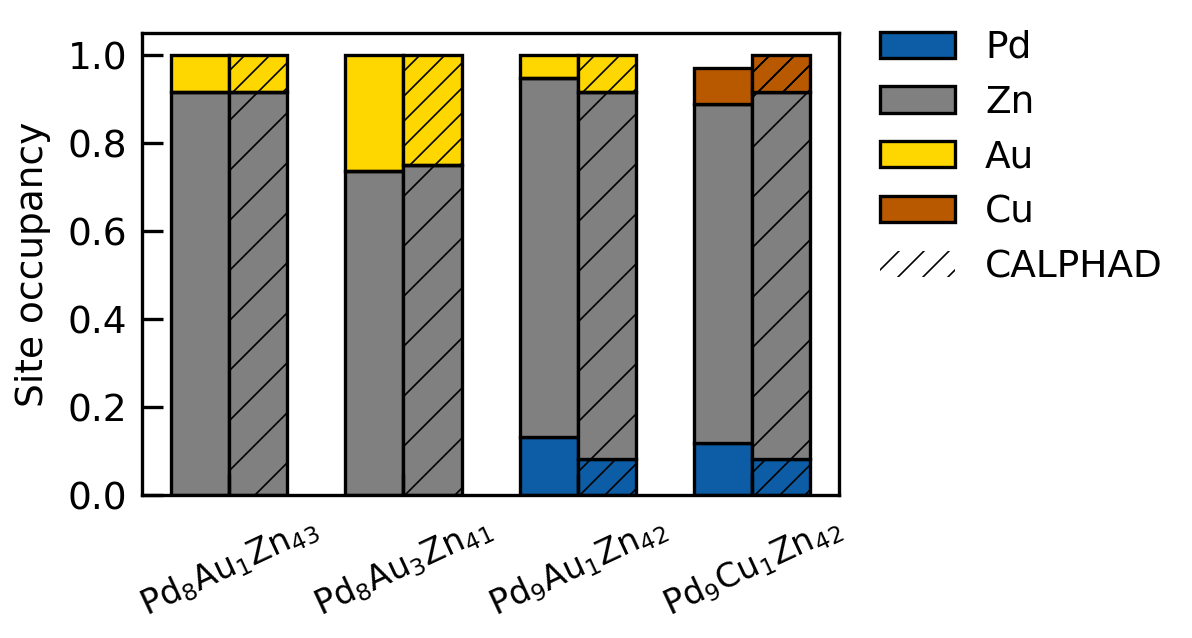
\includegraphics[width=0.8\linewidth]{intermetallics/Intermetallics-PdZnM-SFCalExp.png}
    \caption{Site occupancy on the OH site in Pd$_8$Au$_1$Zn$_{43}$, Pd$_8$Au$_3$Zn$_{41}$, Pd$_9$Au$_1$Zn$_{42}$, and Pd$_9$Cu$_1$Zn$_{42}$ from Rietveld refinement results compared with CALPHAD modeling predictions (marked with slashes). The site fraction of Pd is marked in blue, Zn in grey, Au in yellow, and Cu in brown.}
    \label{intermetallics:fig:PdZnM-SFCalExp}
\end{figure}

\section{Summary} \label{intermetallics:sec:Summary}

Thermodynamic modeling of the Pd-Zn system and the M-Pd-Zn (M = Cu, Ag, and Au) based on the CALPHAD approach has been performed. A 4-sublattice model is used to describe the $\gamma$-brass phase in accordance with its four Wyckoff positions providing a better prediction of surface construction and enabling the understanding of active surface ensembles for catalysts. DFT-based first-principles calculations are used to obtain Gibbs energies of endmembers for the $\gamma$-brass phase. In the binary Pd-Zn $\gamma$-brass phase, Pd atoms first occupy the OT sublattice followed by the OH sublattice, as indicated by DFT-based total energy and phonon calculations supported by the bonding distance and force constants analyses and in agreement with experimental data. Site fractions calculated from the CALPHAD modeling as a function of temperature and composition contribute to analyzing surface construction of the Pd-Zn $\gamma$-brass phase. 

Site occupancy in the ternary M-Pd-Zn (M = Cu, Ag, and Au) $\gamma$-brass phases was determined through the CALPHAD modeling approach and Rietveld refinement. Site occupancy calculations are carried out through the Gibbs energy minimization of the $\gamma$-brass phases. CALPHAD modeling predicts an increase in the site fraction of the coinage metals on the OH site upon alloying M into the Pd-Zn $\gamma$-brass phase. The experimental Rietveld refinements verify the CALPHAD modeling predictions, demonstrating a trend that the coinage metals M cannot displace Pd from the OT site and preferentially occupy the OH site by Zn substitution. This observed trend, irrespective of the atomic radius of M, suggests the electronic interaction between the atoms is more likely to govern atomic site occupation preferences in the $\gamma$-brass phase. The introduction of coinage metals M into the Pd-Zn $\gamma$-brass phase, therefore, leads to Pd$^{\rm OT}$-M$^{\rm OH}$-Pd$^{\rm OT}$ trimer moieties isolated from other Pd and M atoms in the bulk structure by Zn atoms. The M-Pd-Zn (M = Cu, Ag, Au) $\gamma$-brass ternary intermetallics, can therefore offer combinations of isolated Pd atoms, Pd$^{\rm OT}$-Pd$^{\rm OH}$-Pd$^{\rm OT}$ and Pd$^{\rm OT}$-M$^{\rm OH}$-Pd$^{\rm OT}$ clusters. These isolated trimers may be exposed on their surfaces. This understanding of site occupancy and the formation of different types of trimer clusters has significant implications for designing intermetallic catalysts. The isolated Pd, Pd trimers, and Pd-M-Pd clusters within the Zn atoms can enhance the selectivity of catalytic reactions, providing a pathway for tailoring the catalytic properties of $\gamma$-brass phases by strategically introducing coinage metals, thereby optimizing their performance for specific catalytic reactions.

\chapter{Thermodynamic modeling of fluoride and chloride molten salts with model selection, uncertainty quantification, and uncertainty propagation} \label{chap:moltensalts}

\section{Introduction} \label{moltensalts:sec:intro}
Chromium (Cr) is one of the key elements in current reference structural materials for fluoride salt reactors, for example, the Hastelloy-N as the container material (72\%Ni-16\%Mo-7\%Cr-5\%Fe in wt.\%) \cite{koger1972evaluation, manly1958metallurgical}. In the fluoride salt environment, Cr in Ni-based alloy is more susceptible to corrosion compared to other metal elements \cite{olson2009materials, ouyang2014long, liu2020corrosion}. For example, Olson et al. \cite{olson2009materials} performed corrosion tests on a number of Ni-based alloys with different Cr alloying contents. They showed the dissolution of Cr into molten salt and correlated the relationship between Cr content and corrosion resistance \cite{olson2009materials}. Ouyang et al. \cite{ouyang2014long} investigated the corrosion behavior of Hastelloy-N in FLiNaK after 100-1000 h at 700 $^o$C, and the aggregate dissolution of Cr was observed. Recently, Liu et al. \cite{liu2020corrosion} studied Hastelloy-N and showed that the corrosion rate of Cr in FLiNaK-CrF$_3$ is higher than that in FLiBe-CrF$_3$ with Cr$^{3+}$ as the product. Thus, it is important to investigate solubility and multivariate distribution patterns of Cr in FLiNaK. The LiF-NaF-KF system has been extensively studied by many researchers in terms of modeling. Chartrand and Pelton \cite{chartrand2001thermodynamic}, Wang et al. \cite{wang2014phase}, and Ard et al. (MSTDB-TC database) \cite{ard2022development} have investigated this system through CALPHAD modeling. However, we noticed that thermodynamic modeling of the FLiNaK-CrF$_3$ system has been performed based on incomplete and empirically estimated thermochemical data by Yin et al. \cite{yin2018thermodynamic, yin2015thermodynamic} and Dumaire et al. \cite{dumaire2021thermodynamic}. A comprehensive study on the thermodynamic properties of all solid and liquid phases in the FLiNaK-CrF$_3$ system is yet to be conducted.

Chloride molten salts have gained significant attention for their potential applications in advanced nuclear reactors and pyroprocessing techniques \cite{sridharan2012thermal, mourogov2006potentialities, iizuka1997actinides}. Effective separation of fission products, such as lanthanides using pyroprocessing techniques, requires a comprehensive understanding of the thermodynamic properties of molten salts. The CALPHAD  modeling approach \cite{liu2020computational, lukas2007computational} is effective in investigating phase equilibrium and thermodynamic properties in multicomponent systems. For the modeling of complex molten salts, various thermodynamic models within the CALPHAD framework have been developed to capture intricate behaviors such as short-range ordering, including the associate model, two-sublattice ionic model, and MQMQA (see Section \ref{method:ssec:liqmodels}). However, systematically comparing these models and selecting the most appropriate model for molten salts remain a challenge due to different physical interpretations and the complexities involved in quantifying model performance.

In the present work, the fluoride system (LiF, NaF, KF, CrF${_2}$)-CrF${_3}$ and the chloride system LiCl-KCl-LaCl${_3}$ are modeled using the CALPHAD method, supplemented with thermochemical data by first-principles calculations. The open-source software tools of ESPEI \cite{bocklund2019espei} and PyCalphad \cite{otis2017pycalphad} were employed for the modeling process, which facilitates Bayesian parameter estimation, UQ, and Bayesian model selection in modeling molten salts. The present work compares thermodynamic models commonly used in CALPHAD modeling for liquid, providing insights into an effective model selection strategy. 

\section{Revisiting thermodynamics in (LiF, NaF, KF, CrF${_2}$)-CrF${_3}$ by first-principles calculations and CALPHAD modeling} \label{moltensalts:sec:FLiNaKCr}
The thermodynamic description of the (LiF, NaF, KF, CrF$_2$)-CrF$_3$ systems has been revisited, aiming for a better understanding of the effects of Cr on the FLiNaK molten salt. First-principles calculations based on DFT were performed to determine the electronic and structural properties of each compound, including the formation enthalpy, volume, and bulk modulus. DFT-based phonon calculations were carried out to determine the thermodynamic properties of compounds, for example, enthalpy, entropy, and heat capacity as functions of temperature. Phonon-based thermodynamic properties show a good agreement with experimental data of binary compounds LiF, NaF, KF, CrF$_3$, and CrF$_2$, establishing a solid foundation to determine thermodynamic properties of ternary compounds as well as to verify results estimated by the Neumann-Kopp rule. Additionally, DFT-based AIMD simulations were employed to predict the mixing enthalpies of liquid salts. Using DFT-based results and experimental data in the literature, the (LiF, NaF, KF, CrF$_2$)-CrF$_3$ system has been remodeled in terms of the CALPHAD approach using the MQMQA for liquid. Calculated phase stability in the present work shows an excellent agreement with experiments, indicating the effectiveness of combining DFT-based total energy, phonon, and AIMD calculations, and CALPHAD modeling to provide the thermodynamic description in complex molten salt systems.

\subsection{Modeling details} \label{moltensalts:ssec:FLiNaKCrmodel}
%%% Compounds information
The (LiF, NaF, KF, CrF$_2$)-CrF$_3$ system includes five binary (endmember) compounds, i.e., LiF, NaF, KF, CrF$_3$ and CrF$_2$, and eight ternary (intermetallic) compounds, i.e., Li$_3$CrF$_6$, Na$_3$CrF$_6$, Na$_5$Cr$_3$F$_{14}$, NaCrF$_4$, K$_3$CrF$_6$, K$_2$CrF$_5$, KCrF$_4$, and K$_2$Cr$_5$F$_{17}$. De Kozak first suggested these ternary compounds \cite{DeKozak1969} and confirmed by structural studies \cite{de1975systeme,miranday1975croissance, sturm1962phase, garcia2014electrostatic, brunton1969crystal, le2003distorted, manaka2011effects, sassoye2006crystal} via the X-ray diffraction (XRD) method, which was summarized by Dumaire et al. \cite{dumaire2021thermodynamic}. However, thermochemical data on these compounds is scarce. Yin et al. \cite{yin2018thermodynamic, yin2015thermodynamic, yin2014thermodynamic} performed DFT calculations at 0 K to determine the formation enthalpies of Li$_3$CrF$_6$, Na$_3$CrF$_6$, Na$_5$Cr$_3$F$_{14}$, NaCrF$_4$, and KCrF$_4$. Dumaire et al. \cite{dumaire2021thermodynamic} estimated the heat capacities of these compounds based on the Neumann-Kopp rule in terms of the compositional average of heat capacity values of the corresponding compounds or elements \cite{leitner2010application}. 

%%% Modeling and First-principles details for compounds
The present work treats the compounds and endmembers in the AF-CrF${_3}$ (A=Li, Na, and K) systems as stoichiometric compounds. Thermodynamic functions of the binary endmembers are taken from the JRC database \cite{konings2020comprehensive}, JANAF tables \cite{chase1982janaf}, IVTAN tables \cite{gurvich1993ivtanthermo}, and SSUB database \cite{sgteurl}. The Gibbs energy can be expressed as 
\begin{equation} \label{ms:eq:Gstoi}
    G_m=\Delta_f H_m^0 (298.15)-T S_m^0 (298.15)+\int_{298.15}^T C_{P,m} dT - T\int_{298.15}^T \dfrac{C_{P,m}}{T} dT
\end{equation}
where $\Delta_f H_m^0 (298.15)$ is the standard formation enthalpy, $S_m^0 (298.15)$ the standard entropy at 298.15 K, and $C_{P,m}$ the heat capacity. The thermodynamic data of ternary compounds, including enthalpy, entropy, and heat capacity are obtained through DFT-based first-principles and phonon calculations (see Section \ref{method:sec:firstprinciples}).

All DFT-based first-principles and phonon calculations in the present work were performed by the VASP \cite{kresse1996efficient} using the open-source software DFTTK \cite{wang2021dfttk}. The projector augmented-wave method (PAW) was used for electron-ion interactions to increase computational efficiency compared with the full potential methods \cite{blochl1994projector, kresse1999ultrasoft}. Electron exchange and correlation effects were described using both the local density approximation (LDA) \cite{perdew1981self} and the GGA \cite{perdew1996generalized}. In addition, the DFT+U approach was employed for 11 compounds containing Cr, i.e., CrF${_2}$, CrF${_3}$, Cr$_2$F$_5$, Li$_3$CrF$_6$, Na$_3$CrF$_6$, Na$_5$Cr$_3$F$_{14}$, NaCrF$_4$, K$_3$CrF$_6$, K$_2$CrF$_5$, KCrF$_4$, K$_2$Cr$_5$F$_{17}$. The effective U values for Cr were selected as 3.7 eV, considering 3$-$4eV was commonly used in the literature \cite{shi2009magnetism, mattsson2019density, huang2022dft}. The spin configurations were also considered for these 11 compounds containing Cr. All possible configurations by varying spin up and spin down of Cr atoms were explored by the ATAT code \cite{van2009multicomponent}. The spin configuration with the lowest energy for each Cr-containing compound was used for DFT and phonon calculations. Using DFTTK, structure information is the only required input, then robust relaxation schemes can be automatically performed to obtain equilibrium results at 0 K and thermodynamic properties at finite temperatures through the QHA. During DFTTK calculations, the plane-wave cutoff energy was set as 520 eV. Table \ref{ms:tab:DFTdetails} lists the k-points meshes for DFT-based total energy calculations, the supercell sizes and the k-points meshes for phonon calculations. The phonon DOS was analyzed using the YPHON code \cite{wang2014yphon}, which has been integrated into DFTTK \cite{wang2021dfttk}. 

\begin{table}[H]
    \centering
    \caption{Details of DFT-based first-principles calculations for each compound or phase, including space group, total atoms in the supercells, k-point meshes for structure relaxations, and the final static calculations (indicated by DFT), supercell sizes for phonon calculations, k-point meshes for phonon calculations.}
    \begin{tabular}{>{\raggedright\arraybackslash}m{2.5cm}>{\raggedright\arraybackslash}m{2cm}>{\raggedright\arraybackslash}m{2.5cm}>{\raggedright\arraybackslash}m{2.5cm}>{\raggedright\arraybackslash}m{2.8cm}>{\raggedright\arraybackslash}m{2.5cm}}
    \hline
     \textbf{Phase}&\textbf{Space group}&\textbf{Atoms in crystallographic cell}&\textbf{k-points for DFT}&\textbf{Atoms in supercell for phonon}&\textbf{k-points for phonon}\\
    \hline
        LiF&$Fm\Bar{3}m$&8&$10\times10\times10$&32&$10\times10\times10$\\
        NaF&$Fm\Bar{3}m$&8&$10\times10\times10$&32&$10\times10\times10$\\
        KF&$Fm\Bar{3}m$&8&$10\times10\times10$&32&$10\times10\times10$\\
        CrF${_3}$&$R\Bar{3}c$&24&$9\times9\times3$&24&$9\times9\times3$\\
        CrF${_2}$&$P2_1/c$&6&$14\times10\times9$&24&$13\times10\times9$\\
        Li$_3$CrF$_6$&$C2/c$&60&$2\times2\times2$&60&$2\times2\times2$\\
        Na$_3$CrF$_6$&$P2_1/c$&20&$9\times8\times5$&40&$9\times8\times5$\\
        Na$_5$Cr$_3$F$_{14}$&$P2_1/c$&44&$6\times6\times3$&44&$6\times6\times3$\\
        NaCrF$_4$&$P2_1/c$&24&$6\times8\times5$&24&$6\times8\times6$\\
        K$_3$CrF$_6$&$Fm\Bar{3}m$&40&$5\times5\times5$&40&$5\times5\times5$\\
        K$_2$CrF$_5$&$Pbcn$&128&$3\times1\times1$&128&$3\times1\times1$\\
        KCrF$_4$&$Pnma$&144&$3\times1\times1$&144&$3\times1\times1$\\
        K$_2$Cr$_5$F$_{17}$&$Cmcm$&96&$2\times2\times2$&96&$2\times2\times2$\\
        Cr$_2$F$_5$&$C2/c$&28&$6\times6\times6$&N/A&N/A\\
    \hline
    \end{tabular}
    \label{ms:tab:DFTdetails}
\end{table}

%%% CALPHAD modeling details
The MQMQA \cite{pelton2001modified} is used to describe the liquid phase by considering the short-range ordering (SRO) that occurs in liquid salts. Here, the model (A, Cr)(F) is introduced and hence the A$_2$F$_2$, Cr$_2$F$_2$, and ACrF$_2$ quadruplets (A=Li, Na, and K) are formed to consider the interactions among them. Coordination numbers Z describe the SNN coordination number of the species $i$ (= Li, Na, K, Cr, or F) in quadruplets. Z of anions can be calculated to maintain charge neutrality as follows:
\begin{equation} \label{ms:eq:MQMZ}
    \dfrac{q_A}{(Z_{AB:FF}^A)}+\dfrac{q_B}{(Z_{AB:FF}^B)}=2\times \dfrac{q_F}{(Z_{AB:FF}^F)}
\end{equation}
where $q_i$ is the charges of ion $i$ (= Li, Na, K, Cr, or F). Table \ref{ms:tab:CrZ} shows the coordination numbers used in the present work.

\begin{table}[H]
    \centering
    \caption{Coordination number used in the present CALPHAD modeling work with MQMQA for the liquid phase.}
    \begin{tabular}{>{\raggedright\arraybackslash}m{2.5cm}>{\raggedright\arraybackslash}m{2.5cm}>{\raggedright\arraybackslash}m{2.5cm}>{\raggedright\arraybackslash}m{2.5cm}>{\raggedright\arraybackslash}m{2.5cm}}
    \hline
    \textbf{A}&\textbf{B}&\textbf{$Z_{AB:FF}^A$}&\textbf{$Z_{AB:FF}^B$}&\textbf{$Z_{AB:FF}^F$}\\
    \hline
    Li$^+$&Li$^+$&6&6&6 \\
    Na$^+$&Na$^+$&6&6&6\\
    K$^+$&K$^+$&6&6&6\\
    Cr$^{3+}$&Cr$^{3+}$&6&6&2\\
    Li$^+$&Cr$^{3+}$&2&6&2\\
    Na$^+$&Cr$^{3+}$&4&6&2.7\\
    K$^+$&Cr$^{3+}$&6&6&3\\
    Cr$^{2+}$&Cr$^{3+}$&6&6&2.4\\
    Cr$^{2+}$&Cr$^{2+}$&6&6&3\\
    \hline
    \end{tabular}
    \label{ms:tab:CrZ}
\end{table}

The excess Gibbs energy $G^{excess}$ relates to the formation Gibbs energy of the quadruplet, $\Delta g_{quadruplet}^{ex}$, by considering the following reaction:
\begin{equation} \label{ms:eq:MQMGrea}
    \left(\rm {A_2F_2}\right)_{quad}+\left({\rm Cr_2F_2}\right)_{quad}=2\left({\rm ACrF_2}\right)_{quad}\;\;\;\;\;\Delta g_{\rm ACr:F_2}^{ex}
\end{equation}
where $\Delta g_{\rm ACr:F_2}^{ex}$ represents the Gibbs energy change when forming the quadruplet and can be described by:
\begin{equation} \label{ms:eq:MQMGex}
    \Delta g_{\rm {ACr:F_2}}^{ex}=\Delta g_{\rm {ACr:F_2}}^o+\sum_{(i+j)\geq1} g_{\rm {ACr:F_2}}^{ij}\chi _{\rm {ACr:F_2}}^{i}\chi _{\rm {CrA:F_2}}^{j}
\end{equation}
where $g_{\rm {ACr:F_2}}^{ij}$ is a function of temperature and it is independent of composition. $\chi _{\rm {ACr:F_2}}^{i}$ and $\chi _{\rm {CrA:F_2}}^{j}$ are composition-dependent terms as:
\begin{equation} \label{ms:eq:chi}
    \chi_{\rm {ACr:F_2}} = \dfrac{X_{\rm {A_2:F_2}}}{X_{\rm {A_2:F_2}}+X_{\rm {ACr:F_2}}+X_{\rm {Cr_2:F_2}}}
\end{equation}
where $X_{\rm{ACr:F_2}}$ is the fractions of $\left(\rm{ACr:F_2}\right)_{quad}$ shown in (\ref{ms:eq:MQMGrea}). 

In the CrF${_2}$-CrF${_3}$ system, there are three solid solution phases, i.e., CrF${_2}$ near the Cr-rich region, CrF${_3}$ near the F-rich region, and Cr$_2$F$_5$ showing on the middle region of the CrF${_2}$-CrF${_3}$ phase diagram. The present work adopts the same models used by Dumaire et al. \cite{dumaire2021thermodynamic}, where the regular solution model with the Kohler-Toop interpolation \cite{kohler1960estimation, toop1965predicting, chartrand2000choice, pelton2001general} is used for Cr$_2$F$_5$. For solid solution phases near CrF${_2}$ and CrF${_3}$, the sublattice model is used for each phase, respectively, considering the Wyckoff positions of CrF${_2}$ and CrF${_3}$ as follows. CrF${_2}$ possesses the symmetry with space group $P2_1/c$ with two Wyckoff sites of 2a and 4e, and the sublattice model (Cr, Va)$_1$(F, Va)$_2$ is hence used with Va representing the vacancy. CrF${_3}$ phase is modeled by (Cr, Va)$_1$(F, Va)$_3$ by considering its space group $R\bar{3}c$ and the two Wyckoff sites of 2b and 6e. The Gibbs energy is formulated as:
\begin{equation} \label{ms:eq:Crssoln}
    \begin{aligned}
        G_m&=\sum_{i=Cr,Va}{\sum_{j=F,Va}{y_i^\prime y_j^{\prime\prime}}\:^oG_{i:j}}\\
        &+RT\left(\sum_{i=Cr,Va}{y_i^\prime\ln{\left(y_i^\prime\right)}}+\sum_{j=F,Va}{y_j^{\prime\prime}\ln{\left(y_j^{\prime\prime}\right)}}\right)\\&+y_{Cr}^\prime y_{Va}^\prime\left(y_F^{\prime\prime}L_{Cr,Va:F}\right)+y_F^{\prime\prime}y_{Va}^{\prime\prime}\left(y_{Cr}^\prime L_{Cr:F,Va}\right)
    \end{aligned}
\end{equation}
where $y_i^{(s)}$ is the site fraction of component i on sublattice s, ${^o}G_{i:j}$ the Gibbs energy of the endmember (i:j), and $L$ the interaction parameters which can be expanded using the Redlich-Kister polynomials \cite{redlich1948algebraic}. 

Phase equilibria in the LiF-CrF${_3}$, NaF-CrF${_3}$, and KF-CrF${_3}$ binary systems were investigated by De Kozak \cite{de1975systeme, DeKozak1969} using differential thermal analysis (DTA). In LiF-CrF${_3}$, two eutectic reactions were measured, i.e., Liquid $\leftrightarrow$ LiF + Li$_3$CrF$_6$ at 1003 K and around mole fraction $x$(CrF${_3}$) = 0.15 and Liquid $\leftrightarrow$ CrF${_3}$ + Li$_3$CrF$_6$ at 1059 K and $x$(CrF${_3}$) = 0.35. In NaF-CrF${_3}$, one peritectic reaction of Liquid + CrF${_3}$ $\leftrightarrow$ NaCrF$_4$ at 1234 K and three eutectic reactions were determined, i.e., Liquid $\leftrightarrow$ NaCrF$_4$ + Na$_5$Cr$_3$F$_{14}$ at 1133 K, Liquid $\leftrightarrow$ Na$_3$CrF$_6$ + Na$_5$Cr$_3$F$_{14}$ at 1143 K, and Liquid $\leftrightarrow$ Na$_3$CrF$_6$ + NaF at 1166 K and around $x$(CrF${_3}$) = 0.123. In KF-CrF${_3}$, De Kozak \cite{de1975systeme, DeKozak1969} reported three peritectic reactions and two eutectic reactions, i.e., Liquid + CrF${_3}$ $\leftrightarrow$ K$_2$Cr$_5$F$_{17}$ at 1390 K, Liquid + K$_3$CrF$_6$ $\leftrightarrow$ K$_2$CrF$_5$ at 1133 K, and Liquid + K$_2$Cr$_5$F$_{17}$ $\leftrightarrow$ KCrF$_4$ at 1200 K, and Liquid $\leftrightarrow$ K$_3$CrF$_6$ + KF at 1115 K and around $x$(CrF${_3}$) = 0.048, and Liquid $\leftrightarrow$ K$_2$CrF$_5$ + KCrF$_4$ at 1112 K and around $x$(CrF${_3}$) = 0.45. Sturm \cite{sturm1962phase} reported phase equilibria in CrF${_2}$-CrF${_3}$ via quenching experiments and suggested one solid solution phase in CrF${_2}$-CrF${_3}$ with composition of CrF${_3}$ between 0.42 and 0.46 (near Cr$_2$F$_5$). However, the stability of this Cr$_2$F$_5$ solid solution phase was not explored in temperatures below 1023 K. The melting point of Cr$_2$F$_5$ was determined to be around 1270 K \cite{sturm1962phase}. Sturm \cite{sturm1962phase} reported one eutectic reaction, Liquid $\leftrightarrow$ CrF${_2}$ + Cr$_2$F$_5$ at 1103 K around $x$(CrF${_3}$) = 0.14, and one peritectic reaction Liquid + CrF${_3}$ $\leftrightarrow$ Cr$_2$F$_5$ at 1272 K around $x$(CrF${_3}$) = 0.29. Two solid solution phases near the endmembers CrF${_3}$ and CrF${_2}$ were identified from $x$(CrF${_3}$) = 0$-$0.01 and $x$(CrF${_3}$) = 0.90$-$1, respectively. 

Machine learning (ML) was used to estimate more phase equilibria data in terms of a graphic neural network model developed by Hong et al. \cite{hong2022melting} to predict melting points of compounds with composition as input. Melting temperatures of the present ternary compounds including Li$_3$CrF$_6$, Na$_3$CrF$_6$, Na$_5$Cr$_3$F$_{14}$, NaCrF$_4$, K$_3$CrF$_6$, K$_2$CrF$_5$, KCrF$_4$, and K$_2$Cr$_5$F$_{17}$ are estimated by this ML model \cite{hong2022melting}. 

%%%AIMD
For the liquid phase, experimental data such as mixing enthalpy are not available in the AF-CrF${_3}$ (A=Li, Na, and K) systems. Instead, Yin et al. \cite{yin2018thermodynamic, yin2015thermodynamic, yin2014thermodynamic} applied an empirical model to estimate the mixing enthalpy of liquid from the parameters of ions such as ionic radius. In the present work, AIMD simulations were performed to obtain the mixing enthalpy of liquid by VASP \cite{kresse1996efficient}. The supercells containing 108 or 128 atoms with periodic boundaries were used for at least six different compositions in the AF-CrF${_3}$ (A= Li, Na, and K) systems, including A$_{64}$F$_{64}$, A$_{42}$Cr$_6$F$_{60}$, A$_{36}$Cr$_9$F$_{63}$, A$_{32}$Cr$_{16}$F$_{80}$, A$_{18}$Cr$_{18}$F$_{72}$, A$_{16}$Cr$_{24}$F$_{88}$, A$_{10}$Cr$_{22}$F$_{76}$, and Cr$_{32}$F$_{96}$ (A=Li, Na, and K). The NVT canonical ensemble (i.e., the fixed number of atoms N, volume V, and temperature T) with a Nosé thermostat for temperature control \cite{nose1984unified} was employed in the present work. The temperature for each supercell was set as 1700 K, which is above all the temperatures of liquidus in the AF-CrF${_3}$ (A= Li, Na, and K) systems. A single $\Gamma$ point $1\times1\times1$ was used as the k-point mesh, together with a 400 eV cutoff energy. During AIMD simulations, Newton’s equation of motion was solved via the Verlet algorithm with a time step of 2 fs, and each calculation is run for 10,000 steps to reach thermal equilibrium.

%%%CALPHAD modeling
Thermodynamic modeling of the (LiF, NaF, KF, CrF${_2}$)-CrF${_3}$ system was carried out using the open-source software ESPEI \cite{bocklund2019espei} and PyCalphad \cite{otis2017pycalphad} with the newly implemented MQMQA \cite{palma2023thermodynamic}. All model parameters were simultaneously optimized through the Bayesian approach using MCMC \cite{bocklund2019espei}. The input data were primarily experimental phase equilibrium data including two or more co-existing phases. For stochiometric compounds, their thermochemical data from DFT-based calculations were also used as input. For the liquid phase, its mixing enthalpy from AIMD calculations was used as input for refining model parameters. In the present work, each model parameter employed two Markov chains with a standard derivation of 0.1 when initializing its Gaussian distribution. During the modeling process, the chain values can be tracked and the MCMC processes were performed until the model parameters converged.

\subsection{Thermodynamic properties in (LiF, NaF, KF, CrF$_2$)-CrF$_3$ by first-principles calculations} \label{moltensalts:ssec:FLiNaKCrsolids}

Table \ref{ms:tab:CrEOS} shows the predicted equilibrium properties of V$_0$, B$_0$, and B$^\prime$ by the EOS E-V fitting at 0 K in comparison with experimental bulk moduli \cite{yagi1978experimental, haussuhl1960thermo, boehler1980thermal, rao1974anderson, bensch1972third, jorgensen2004compression}. The B$_0$ results from GGA show a good agreement with experimental measurements. For the LiF compound, GGA predicts B$_0$ = 67.6 GPa and B$^\prime$ = 4.17, aligning well with the measured values of 65.4 GPa and 4.98 by Boehler et al. \cite{boehler1980thermal}. In comparison with the three measured B$_0$ values of 66.5 GPa by Yagi \cite{yagi1978experimental}, 76.9 GPa by Haussühl \cite{haussuhl1960thermo}, and 65.4 GPa by Boehler et al. \cite{boehler1980thermal}, the B$_0$ result by GGA shows a mean absolute error (MAE) of 4.2 GPa, while LDA predicts B$_0$ = 86.5 GPa with a higher MAE of 16.9 GPa. Considering the NaF compound, GGA predicts B$_0$ = 45.0 GPa, matching with the measured 45.9 GPa by Yagi \cite{yagi1978experimental} but lower than the measured values of 53.8 GPa by Haussühl \cite{haussuhl1960thermo}, 52.3 GPa by Rao \cite{rao1974anderson}, and 48.2 GPa by Bensch et al. \cite{bensch1972third} with the MAE around 5 GPa. On the other hand, LDA predicts B$_0$ = 61.4 GPa, which is higher than the experimental B$_0$ \cite{yagi1978experimental, haussuhl1960thermo, rao1974anderson, bensch1972third} with MAE = 11.4 GPa. Additionally, for the B$^\prime$ values of NaF, LDA predicts B$^\prime$ = 4.74, which is higher than the predicted 4.60 by GGA and closer to 5.89 reported by Bensch et al. \cite{bensch1972third}. Regarding the KF compound, the measured B$_0$ values (37.0 GPa by Yagi \cite{yagi1978experimental} and 35.5 GPa by Haussühl \cite{haussuhl1960thermo}) fall between the LDA result of 43.5 GPa and the GGA result of 28.9 GPa. The MAE value of LDA with respect to the measured B$_0$ values is 7.25 GPa, slightly lower than MAE = 7.35 GPa by GGA. As for the CrF$_3$ compound, GGA+U reports B$_0$ = 29.3 GPa, showing a 0.3\% difference compared to 29.2 GPa measured by Jørgensen et al. \cite{jorgensen2004compression}. LDA+U predicts B$_0$ = 46.2 GPa, which is 58\% higher than the measured 29.2 GPa \cite{jorgensen2004compression}. The present results indicate that LDA predicts smaller V$_0$ and higher B$_0$ values than those from GGA. It is consistent with the previous observations that LDA tends to underestimate lattice constants and overestimate cohesive energy with respect to GGA \cite{haas2009calculation, he2014accuracy}.

\begin{table}[H]
    \centering
    \caption{Predicted equilibrium properties of volume V$_0$, bulk modulus B$_0$, and the first derivative of bulk modulus with respect to pressure B$^\prime$ for each compound based on the present EOS fitting at 0 K in the FLiNaK-CrF$_3$-CrF$_2$ system. Experimental data (marked with *) \cite{yagi1978experimental, haussuhl1960thermo, boehler1980thermal, rao1974anderson, bensch1972third, jorgensen2004compression} are also listed for comparison}
    \begin{tabular}{>{\raggedright\arraybackslash}m{2.5cm}>{\raggedright\arraybackslash}m{4cm}>{\raggedright\arraybackslash}m{3cm}>{\raggedright\arraybackslash}m{2cm}>{\raggedright\arraybackslash}m{2cm}}
    \hline
    \textbf{Phases}&\textbf{Method}&\textbf{V$_0$} (\r{A}$^3$/atom)&\textbf{B$_0$}&\textbf{B$^\prime$}\\
    \hline
    LiF&LDA&7.488&86.5&4.25\\
    &GGA&8.419&67.6&4.17\\
    &Yagi$^*$\cite{yagi1978experimental}&&66.5&\\
    &Haussühl$^*$\cite{haussuhl1960thermo}&&76.9&\\
    &Boehler et al.$^*$ \cite{boehler1980thermal}&&65.4&4.98\\
    NaF&LDA&11.457&61.4&4.74\\
	&GGA&13.020&45.0&4.60\\
    &Yagi$^*$\cite{yagi1978experimental}&&45.9&\\
    &Haussühl$^*$\cite{haussuhl1960thermo}&&53.8&\\
    &Ramji Rao$^*$\cite{rao1974anderson}&&52.3&\\	
    &Bensch et al.$^*$ \cite{boehler1980thermal}&&48.2&5.89\\
    KF&LDA&17.363&43.5&5.06\\
	&GGA&20.050&28.9&4.84\\
	&Yagi$^*$\cite{yagi1978experimental}&&37.0&\\
	&Haussühl$^*$\cite{haussuhl1960thermo}&&35.5&\\	
    CrF$_3$&LDA+U&11.152&46.2&8.46\\
	&GGA+U&12.902&29.3&7.29\\
	&Jørgensen et al.$^*$\cite{jorgensen2004compression}&&29.2&10.3\\
    CrF$_2$&LDA+U&12.443&71.1&2.74\\
    Li$_3$CrF$_6$&LDA+U&9.543&56.1&5.85\\
    Na$_3$CrF$_6$&LDA+U&11.577&57.5&5.46\\
    Na$_5$Cr$_3$F$_{14}$&LDA+U&11.757&52.2&5.15\\
    NaCrF$_4$&LDA+U&11.933&53.0&4.35\\
    K$_3$CrF$_6$&LDA+U&15.705&51.5&5.67\\
    K$_2$CrF$_5$&LDA+U&13.858&45.9&5.65\\
    KCrF$_4$&LDA+U&13.920&38.1&4.88\\
    K$_2$Cr$_5$F$_{17}$&LDA+U&13.314&49.3&6.91\\
    Cr$_2$F$_5$&LDA+U&12.225&46.6&7.91\\
    \hline
    \end{tabular}
    \label{ms:tab:CrEOS}
\end{table}

Figure \ref{ms:fig:FLiNaKCrphonon} compares the phonon DOS of LiF, NaF, and KF obtained using LDA and GGA in comparison with direct measurements by neutron scattering \cite{dolling1968lattice, buhrer1970lattice} or fittings in terms of measurements \cite{karo1969lattice}. Overall, the peak positions of the experimental phonon DOS are well reproduced by both LDA and GGA. However, in the low-frequency region (e.g., < 5 THz for LiF and NaF, and < 3 THz for KF), the phonon DOS predicted by LDA show a better match in both the shape and the peak position with respect to experimental data \cite{dolling1968lattice, buhrer1970lattice, karo1969lattice} than those from GGA. This observation suggests that LDA predicts more reliable thermodynamic properties of LiF, NaF, and KF when employing the phonon-based QHA since these properties are mainly regulated by phonon DOS at low-frequency regions \cite{shang2019achieving}. 

\begin{figure}[H]
    \centering
    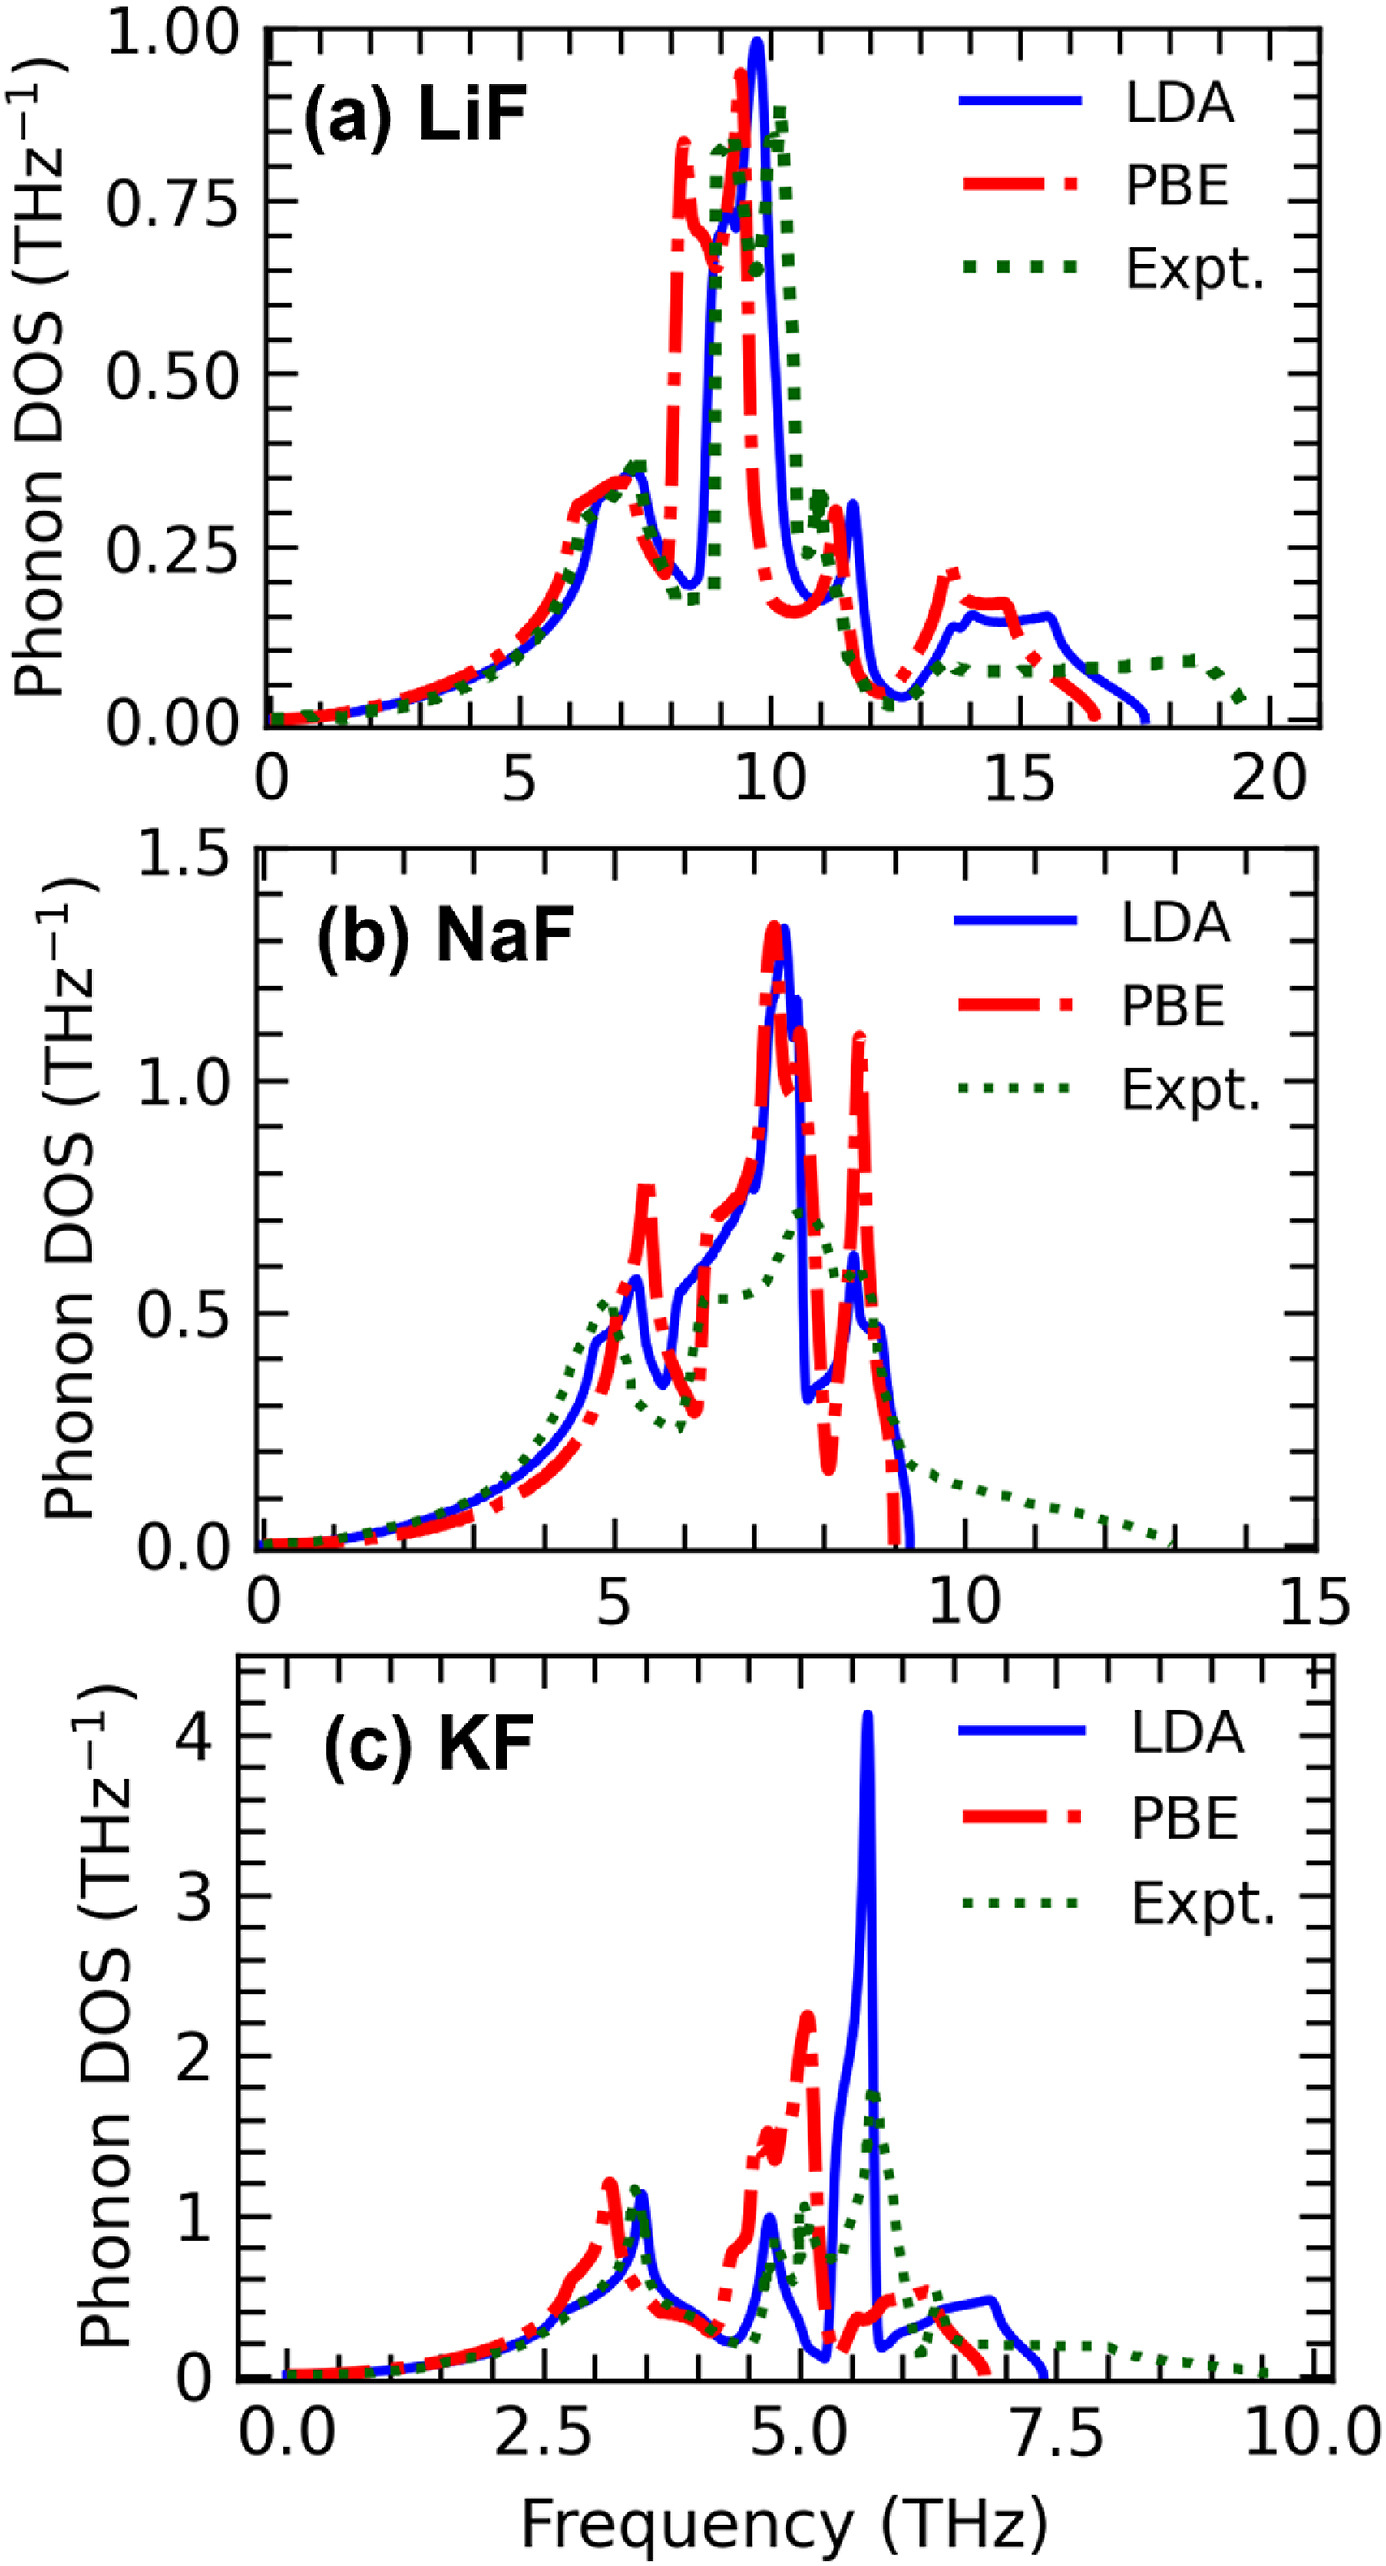
\includegraphics[width=0.45\linewidth]{moltensalts/Moltensalts-FLiNaKCr-PhononDOS.jpg}
    \caption{Predicted phonon density of states (DOS) of (a) LiF, (b) NaF, and (c) KF from DFT-based phonon calculations in comparison with phonon DOS from experiments \cite{dolling1968lattice, buhrer1970lattice, karo1969lattice}. Blue lines show results from the LDA approach, red dot-dashed lines show results from the GGA-PBE approach, and the green dotted lines are results from experiments \cite{dolling1968lattice, buhrer1970lattice, karo1969lattice}. }
    \label{ms:fig:FLiNaKCrphonon}
\end{figure}

Figure \ref{ms:fig:FLiNaKCr-Benchmark} illustrates a comparison of the predicted heat capacity (C$_p$), entropy (S), and enthalpy (H$-$H$_{300}$) of LiF, NaF, and KF in terms of the phonon-based QHA, where the DFT calculations were conducted using both the LDA and GGA, and the predicted results are compared to the data from the SSUB database \cite{sgteurl}. In general, thermodynamic properties predicted by LDA align well with the results from SSUB. The most substantial difference between LDA and SSUB is the C$_p$ values of KF, where a 6\% disparity is noted. Furthermore, these comparisons reveal that the LDA results exhibit a better agreement with SSUB than the GGA results, particularly for LiF. For example, at 1100 K, the C$_p$ values predicted by LDA demonstrate only a 2\% difference compared to those from the SSUB \cite{sgteurl}, whereas an 18\% difference is observed when using GGA. Figure \ref{ms:fig:FLiNaKCr-Benchmark} indicates that the QHA in terms of LDA yields more reliable predictions of thermodynamic properties in LiF-NaF-KF-based system, agreeing with the observations in phonon DOS in Figure \ref{ms:fig:FLiNaKCrphonon}. Subsequent DFT calculations were hence performed using the LDA approach. 

\begin{figure}[ht]
    \centering
    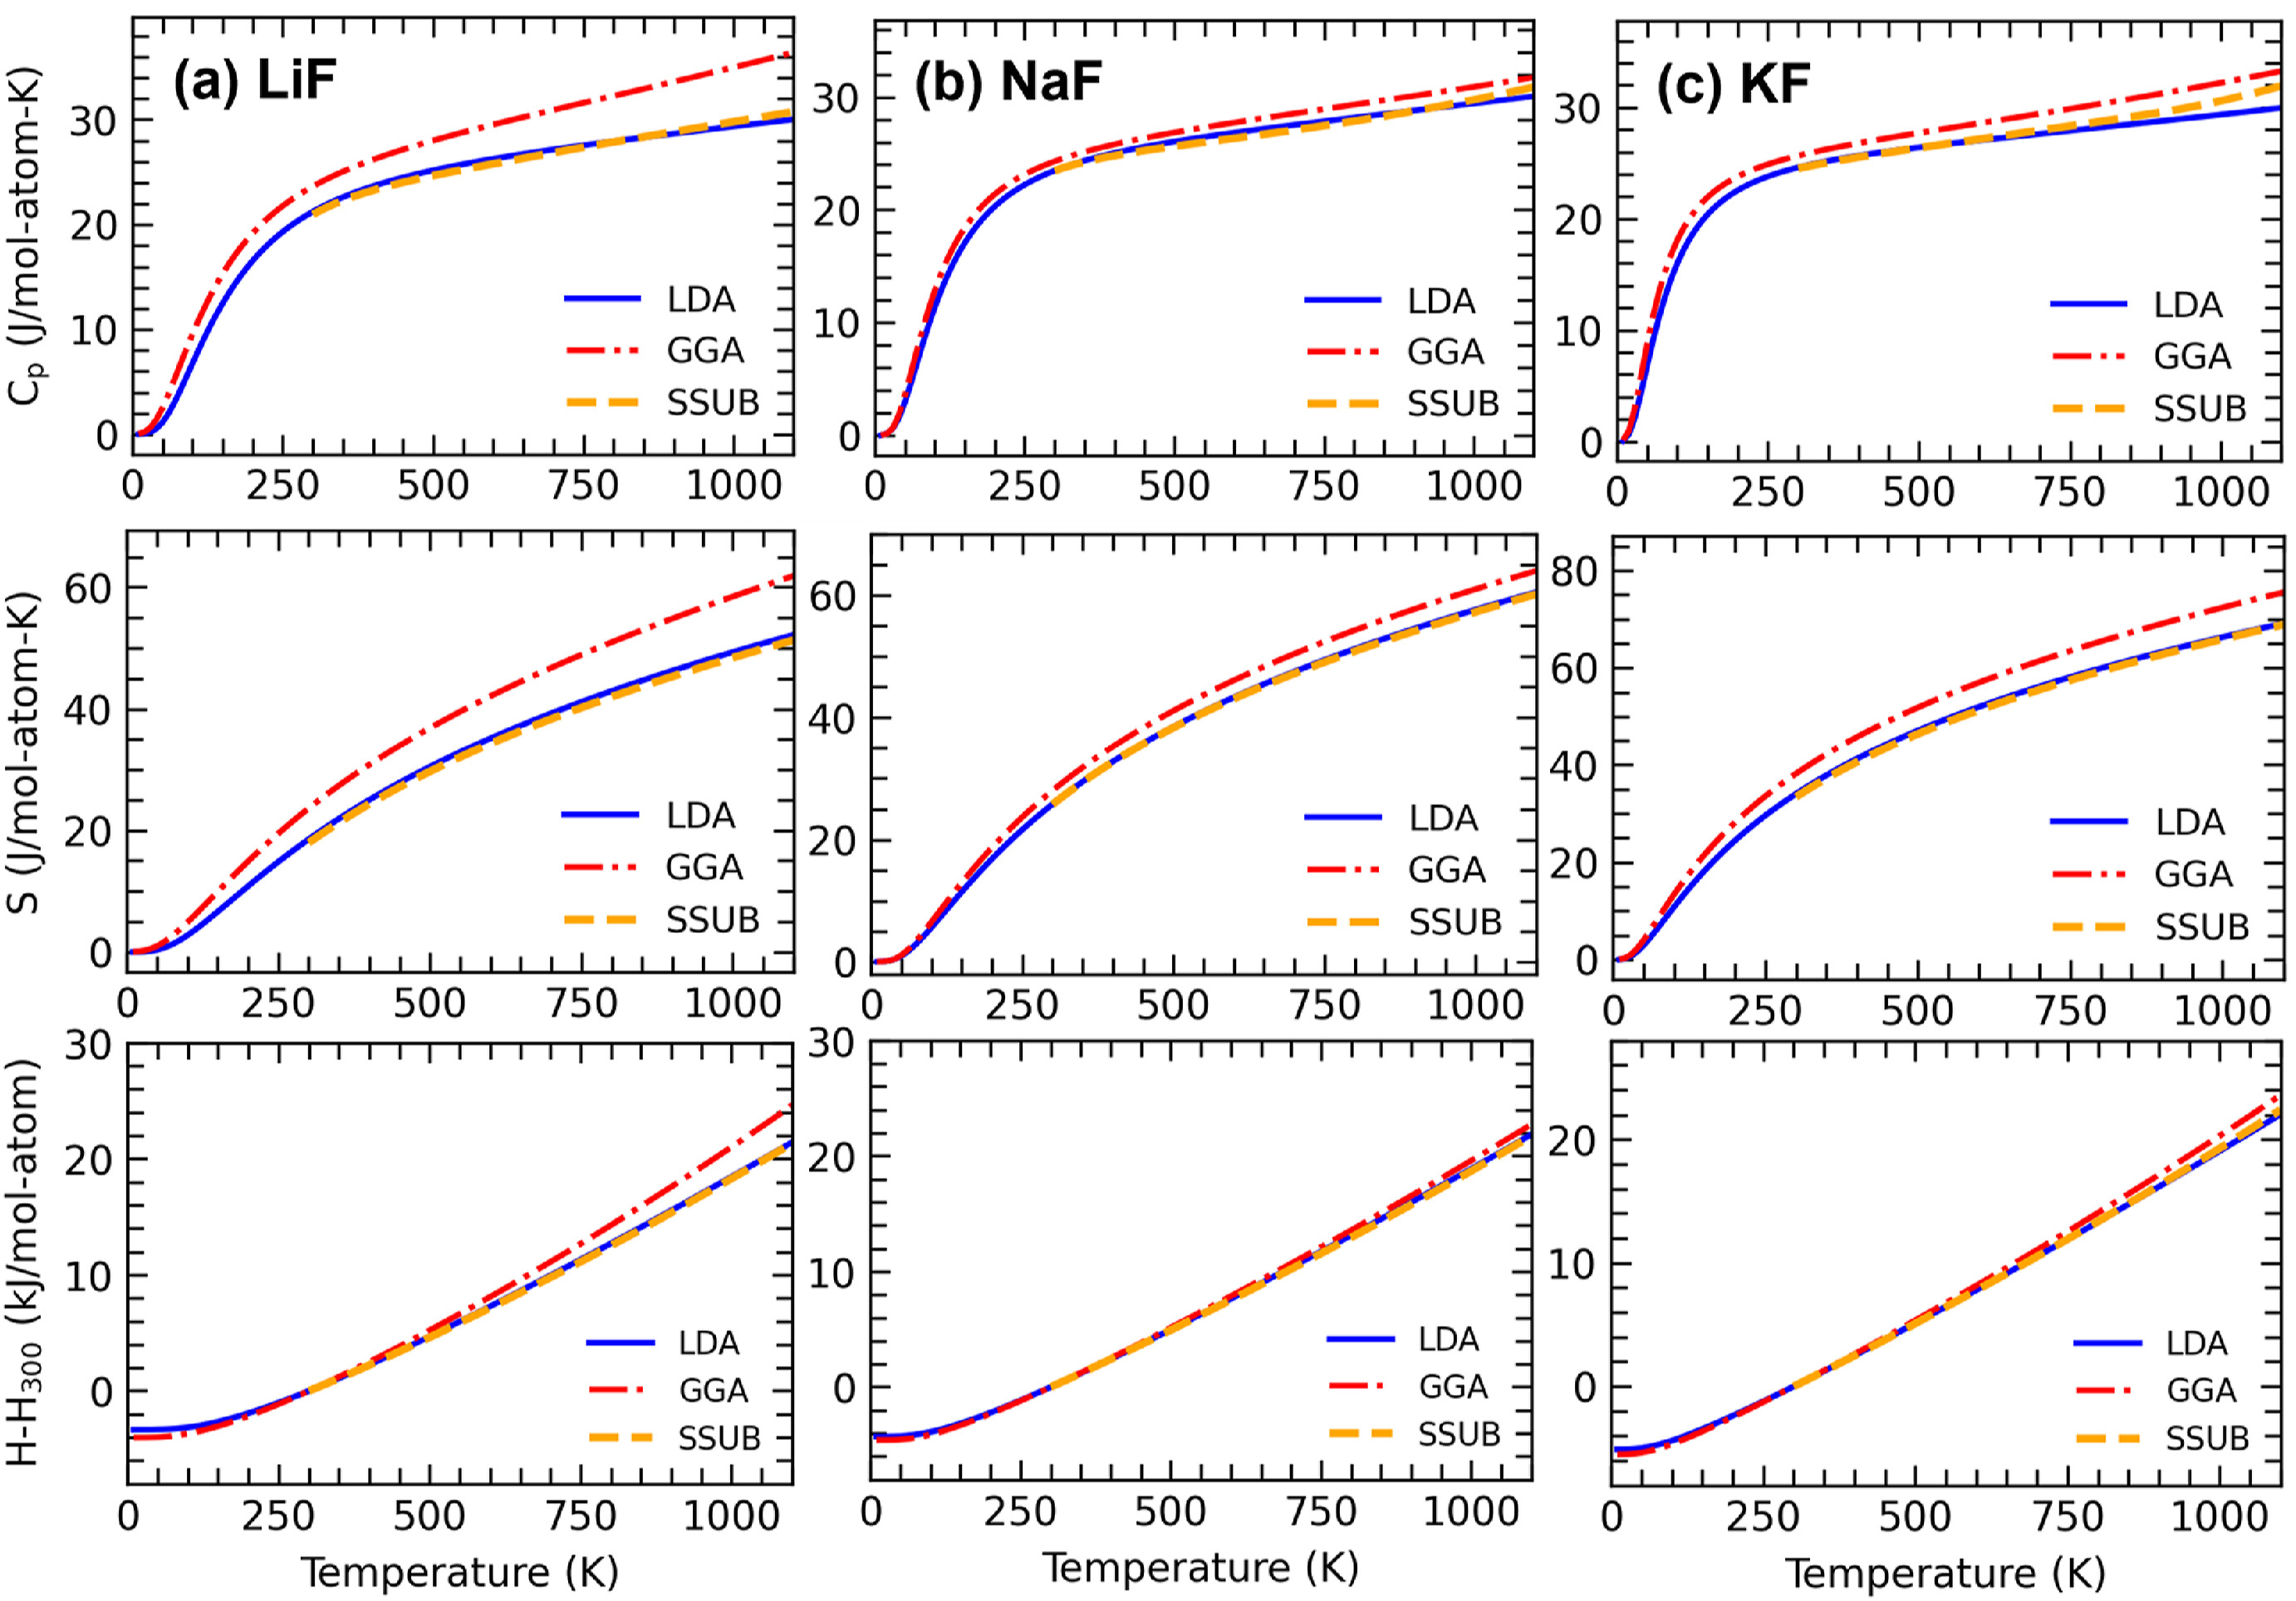
\includegraphics[width=1\linewidth]{moltensalts/Moltensalts-FLiNaKCr-Benchmark.jpg}
    \caption{Predicted heat capacity C$_p$, entropy S, and enthalpy with reference at 300 K (H$-$H$_{300}$) of (a) LiF, (b) NaF, and (c) KF by DFT-based QHA via phonon calculations. Results by LDA is marked as solid blue lines, calculations by PBE are marked as dashed dot red lines, and the SSUB results \cite{sgteurl} are in dashed yellow lines. The SSUB results are implemented in the present modeling work.}
    \label{ms:fig:FLiNaKCr-Benchmark}
\end{figure}

Figure \ref{ms:fig:FLiNaKCr-Benchmark-Cr} shows the present DFT predictions and the values in SSUB \cite{sgteurl} regarding C$_p$, S, and H$-$H$_{300}$ for CrF$_3$ and CrF$_2$. In general, the present predictions tend to be lower than those obtained from SSUB \cite{sgteurl}. For CrF$_3$, the DFT predicted C$_p$ = 19.77 J/mol-atom-K closely aligns with the SSUB value of 19.73 J/mol-atom-K at 300 K. As the temperature increases to 1300 K, the difference increases to 9\%. Similarly, for CrF$_2$, the C$_p$ = 21.22 J/mol-atom-K at 300 K by DFT is in good agreement with the value of 21.66 from SSUB. At a higher temperature of 1140 K, the difference expands to 12\%. Regarding entropy, DFT predicts lower S values for both CrF$_3$ and CrF$_2$ than those in SSUB across the temperature range shown in Figure \ref{ms:fig:FLiNaKCr-Benchmark-Cr}. At high temperatures (e.g., 1600 K for CrF$_3$ and 1140 K for CrF$_2$), it shows a 10\% difference in CrF$_3$ and 14\% in CrF$_2$. It is found that a good agreement is observed regarding H$-$H$_{300}$ values of CrF$_3$ and CrF$_2$ between the DFT calculations and the SSUB at lower temperatures (< 1000 K for CrF$_3$ and < 600 K for CrF$_2$). H$-$H$_{300}$ from DFT becomes slightly lower than that in SSUB \cite{sgteurl} with increasing temperature, with the differences, for example, around 5\% in CrF$_3$ at 1650 K and 9\% in CrF$_2$ at 1140 K.

\begin{figure}[ht]
    \centering
    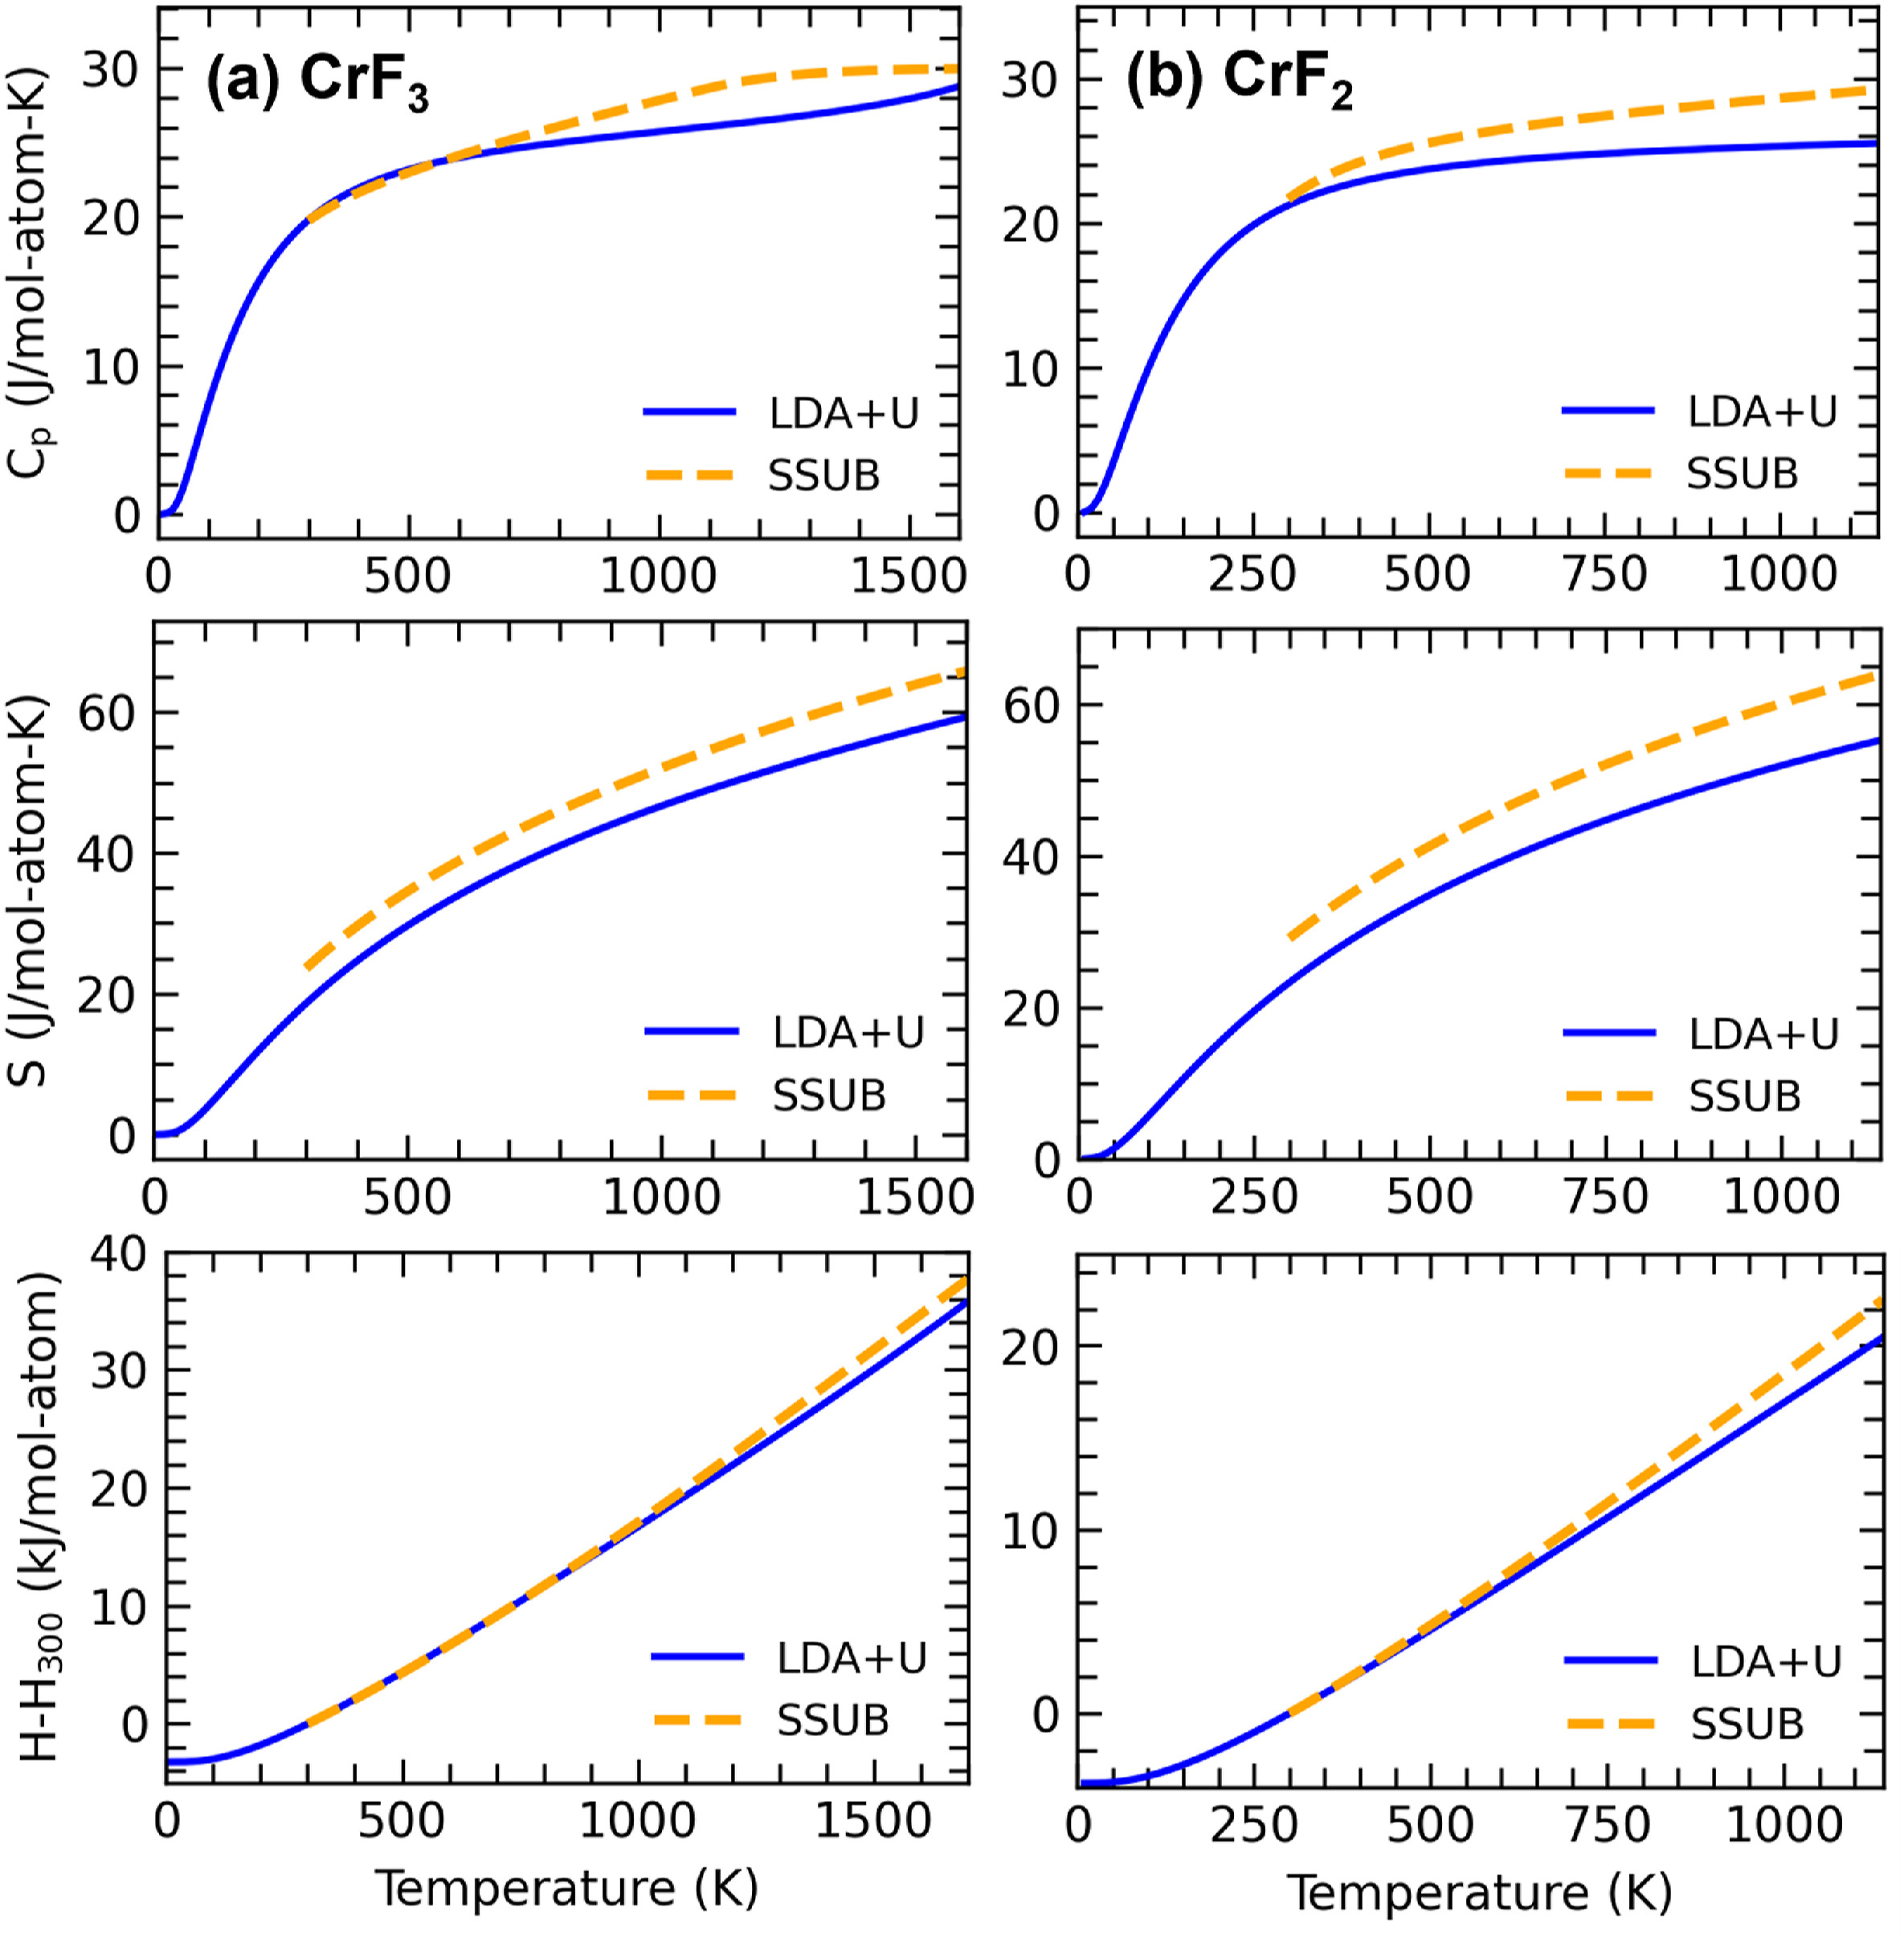
\includegraphics[width=0.75\linewidth]{moltensalts/Moltensalts-FLiNaKCr-Benchmark-Cr.jpg}
    \caption{Predicted heat capacity C$_p$, entropy S, and enthalpy with reference at 300 K (H$-$H$_{300}$) of (a) CrF$_3$ and (b) CrF$_2$ by DFT-based QHA via phonon calculations marked in solid lines in comparison with SSUB \cite{sgteurl} in dashed lines.}
    \label{ms:fig:FLiNaKCr-Benchmark-Cr}
\end{figure}

Table \ref{ms:tab:FLiNaK-Cr-Hf} shows the present DFT values of formation enthalpy ($\Delta_fH_m$) of these ternary compounds using the LDA+U approach, together with the reactions to form these compounds. Table \ref{ms:tab:FLiNaK-Cr-Hf} shows that the $\Delta_fH_m$ values are negative for all ternary compounds with reference to their corresponding binary compounds. Yin et al. \cite{yin2018thermodynamic, yin2014thermodynamic} conducted DFT calculations for Li$_3$CrF$_6$ and Na$_3$CrF$_6$. Predicted $\Delta_fH_m$ values from the Materials Project \cite{jain2013commentary} and the Open Quantum Materials Database (OQMD) \cite{kirklin2015open} are also listed in Table \ref{ms:tab:FLiNaK-Cr-Hf} and displayed in Figure \ref{ms:fig:FLiNaKCr-Hf}. The present DFT calculations by LDA+U predict higher $\Delta_fH_m$ values of Li$_3$CrF$_6$ and Na$_3$CrF$_6$ than those by Yin et al. \cite{yin2018thermodynamic, yin2014thermodynamic} using GGA. The present DFT calculations align better with results from the Materials Project \cite{jain2013commentary} and OQMD \cite{kirklin2015open} than calculations from Yin et al. \cite{yin2018thermodynamic, yin2014thermodynamic}. Figure \ref{ms:fig:FLiNaKCr-Hf} displays the convex hulls for the LiF-CrF$_3$, NaF-CrF$_3$, and KF-CrF$_3$ systems based on the $\Delta_fH_m$ values listed in Table \ref{ms:tab:FLiNaK-Cr-Hf}. These convex hulls serve as indicators regarding the stability of ternary compounds in these systems. Li$_3$CrF$_6$ is on the convex hull, suggesting that it is stable in the LiF-CrF$_3$ system. In the NaF-CrF$_3$ system, Na$_3$CrF$_6$ is located on the hull, indicating its stability at 0 K. Na$_5$Cr$_3$F$_{14}$ shows an elevation of 1.09 kJ/mol-atom above the hull, and NaCrF$_4$ shows 0.42 kJ/mol-atom above the hull. In the KF-CrF$_3$ system, K$_2$CrF$_5$ is on the convex hull at 0 K. K$_2$Cr$_5$F$_{17}$ is the farthest away from the convex hull (1.31 kJ/mol-atom above it), while K$_3$CrF$_6$ and KCrF$_4$ are 0.62 kJ/mol-atom and 0.61 kJ/mol-atom above the hull, respectively. These calculations at 0 K suggest that Na$_5$Cr$_3$F$_{14}$, NaCrF$_4$, K$_2$Cr$_5$F$_{17}$, K$_3$CrF$_6$, and KCrF$_4$ are not stable at 0 K, while De Kozak \cite{DeKozak1969} reported the existence of the above ternary compounds at high temperature. It suggests that phonon-based QHA is necessary to investigate the thermodynamic properties of ternary compounds at high temperatures.

\begin{table}[H]
    \centering
    \caption{DFT-based results of formation enthalpy ($\Delta_fH_m$) at 0 K of ternary compounds in the AF-CrF$_3$ (A=Li, Na, and K) systems with the reference states as shown in the reactions. DFT results from Yin et al. \cite{yin2018thermodynamic, yin2014thermodynamic}, the Materials Project \cite{jain2013commentary}, and the Open Quantum Materials Database (OQMD) \cite{kirklin2015open} are listed for comparison.}
    \begin{tabular}{>{\raggedright\arraybackslash}m{2.5cm}>{\raggedright\arraybackslash}m{5cm}>{\raggedright\arraybackslash}m{3cm}>{\raggedright\arraybackslash}m{5cm}}
    \hline
    \textbf{Compound}&\textbf{Reaction}&\textbf{$\Delta_fH_m$ (J/mol-atom)}&\textbf{Source}\\
    \hline
    Li$_3$CrF$_6$&Li$_3$CrF$_6$$=$3LiF$+$CrF$_3$&$-1815$&This work\\
    &&$-4144$&Yin et al. \cite{yin2014thermodynamic}\\
    &&$-2238$&Materials Project \cite{jain2013commentary}\\
    &&$-2161$&OQMD \cite{kirklin2015open}\\
    Na$_3$CrF$_6$&Na$_3$CrF$_6$$=$3NaF$+$CrF$_3$&$-7849$&This work\\
	&&$-8592$&Yin et al. \cite{yin2018thermodynamic}\\
    &&$-6657$&Materials Project \cite{jain2013commentary}\\
    &&$-8683$&OQMD \cite{kirklin2015open}\\
    Na$_3$CrF$_6$&Na$_3$CrF$_6$$=$3NaF$+$CrF$_3$&$-7849$&This work\\
	&&$-8592$&Yin et al. \cite{yin2018thermodynamic}\\
    &&$-6657$&Materials Project  \cite{jain2013commentary}\\
    &&$-8683$&OQMD \cite{kirklin2015open}\\
    Na$_5$Cr$_3$F$_{14}$&Na$_5$Cr$_3$F$_{14}$$=$5NaF$+$3CrF$_3$&$-5447$&This work\\
	&&$-5148$&Materials Project \cite{jain2013commentary}\\
	&&$-6859$&OQMD \cite{kirklin2015open}\\
    NaCrF$_4$&NaCrF$_4$$=$NaF$+$CrF$_3$&$-4816$&This work\\
    &&$-5071$&Materials Project \cite{jain2013commentary}\\
	&&$-6657$&OQMD \cite{kirklin2015open}\\
    K$_3$CrF$_6$&K$_3$CrF$_6$$=$3KF$+$CrF$_3$&$-8621$&This work\\
    &&$-11038$&Materials Project \cite{jain2013commentary}\\
	&&$-13855$&OQMD \cite{kirklin2015open}\\
    K$_2$CrF$_5$&K$_2$CrF$_5$$=$2KF$+$CrF$_3$&$-12322$&This work\\
	&&$-12446$&Materials Project \cite{jain2013commentary}\\
    KCrF$_4$&KCrF$_4$$=$KF$+$CrF$_3$&$-8631$&This work\\
    &&$-9970$&Materials Project \cite{jain2013commentary}\\
    K$_2$Cr$_5$F$_{17}$&K$_2$Cr$_5$F$_{17}$$=$2KF$+$5CrF$_3$&$-3974$&This work\\
    \hline
    \end{tabular}
    \label{ms:tab:FLiNaK-Cr-Hf}
\end{table}

\begin{figure}[H]
    \centering
    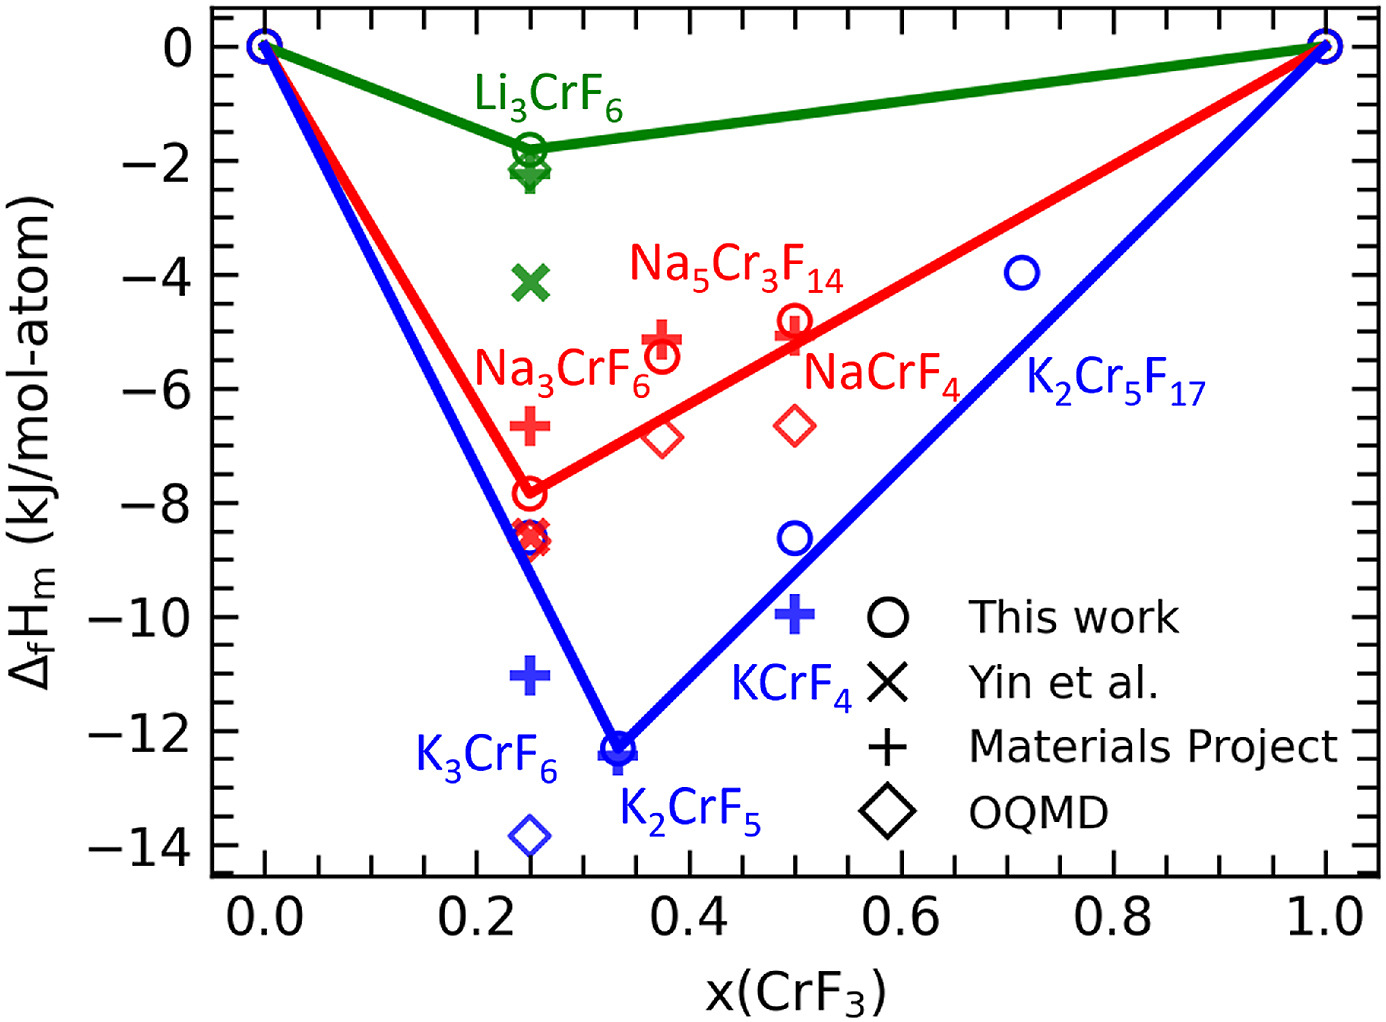
\includegraphics[width=0.5\linewidth]{moltensalts/Moltensalts-FLiNaKCr-DFTHf.jpg}
    \caption{Convex hull of ternary compounds in LiF-CrF$_3$ (green), NaF-CrF$_3$ (red), and KF-CrF$_3$ (blue) at 0 K from DFT-based calculations from the present work. Circles ($\circ$) are the formation enthalpy of compounds from the present work; cross markers ($\times$) are the formation enthalpy of compounds from Yin et al. \cite{yin2018thermodynamic, yin2014thermodynamic}; plus markers ($+$) result from The Materials Project \cite{jain2013commentary}; and diamond markers ($\diamond$) results from OQMD \cite{kirklin2015open}. }
    \label{ms:fig:FLiNaKCr-Hf}
\end{figure}

Figure \ref{ms:fig:FLiNaKCr-DFTcompounds} shows the predicted heat capacities C$_p$ of ternary compounds in the AF-CrF$_3$ (A= Li, Na, and K) systems from the phonon-based QHA, in comparison with the results estimated by the Neumann-Kopp rule \cite{leitner2010application}, which were used in CALPHAD modeling by Dumaire et al. \cite{dumaire2021thermodynamic}. It shows that the Neumann-Kopp rule matches the results of phonon-based QHA in the LiF-CrF$_3$ system. However, in the NaF-CrF$_3$ and KF-CrF$_3$ systems, the Neumann-Kopp rule estimates higher values of C$_p$ with respect to the values predicted by phonon-based QHA. The differences between the LiF-CrF$_3$ system and the NaF/KF-CrF$_3$ may be attributed to variations in melting temperatures between ternary and corresponding binary compounds. For example, in the LiF-CrF$_3$ system, the melting temperature of Li$_3$CrF$_6$ is reported at 1129 K \cite{DeKozak1969}, which is close to that of LiF at 1121 K and below that of CrF$_3$ at 1698 K \cite{sgteurl}. Considering the temperature below the melting point of Li$_3$CrF$_6$ (T < 1129 K), there are reliable resources of C$_p$ data from two endmembers LiF and CrF$_3$, thus the Neumann-Kopp rule C$_p$ estimation of Li$_3$CrF$_6$ is acceptable. However, in the NaF-CrF$_3$ system, Na$_3$CrF$_6$ melts at 1413 K \cite{DeKozak1969}, while NaF melts at 1269 K \cite{sgteurl}, indicating that there is an approximately 150 K temperature range without reliable C$_p$ data for NaF. In contrast, the phonon-based calculations are direct predictions of ternary compounds and they provide more accurate descriptions of thermodynamic properties for compounds than those by the Neumann-Kopp rule used by Dumaire et al. \cite{dumaire2021thermodynamic}, especially at high temperatures. Therefore, the phonon-based QHA results were used in the present CALPHAD modeling to improve the accuracy in describing ternary compounds. Note that the C$_p$ values for compounds in the (LiF, NaF, KF, and CrF$_2$)-CrF$_3$ systems can be predicted using the Supplementary XML file \cite{gong2024revisiting}.

\begin{figure}[H]
    \centering
    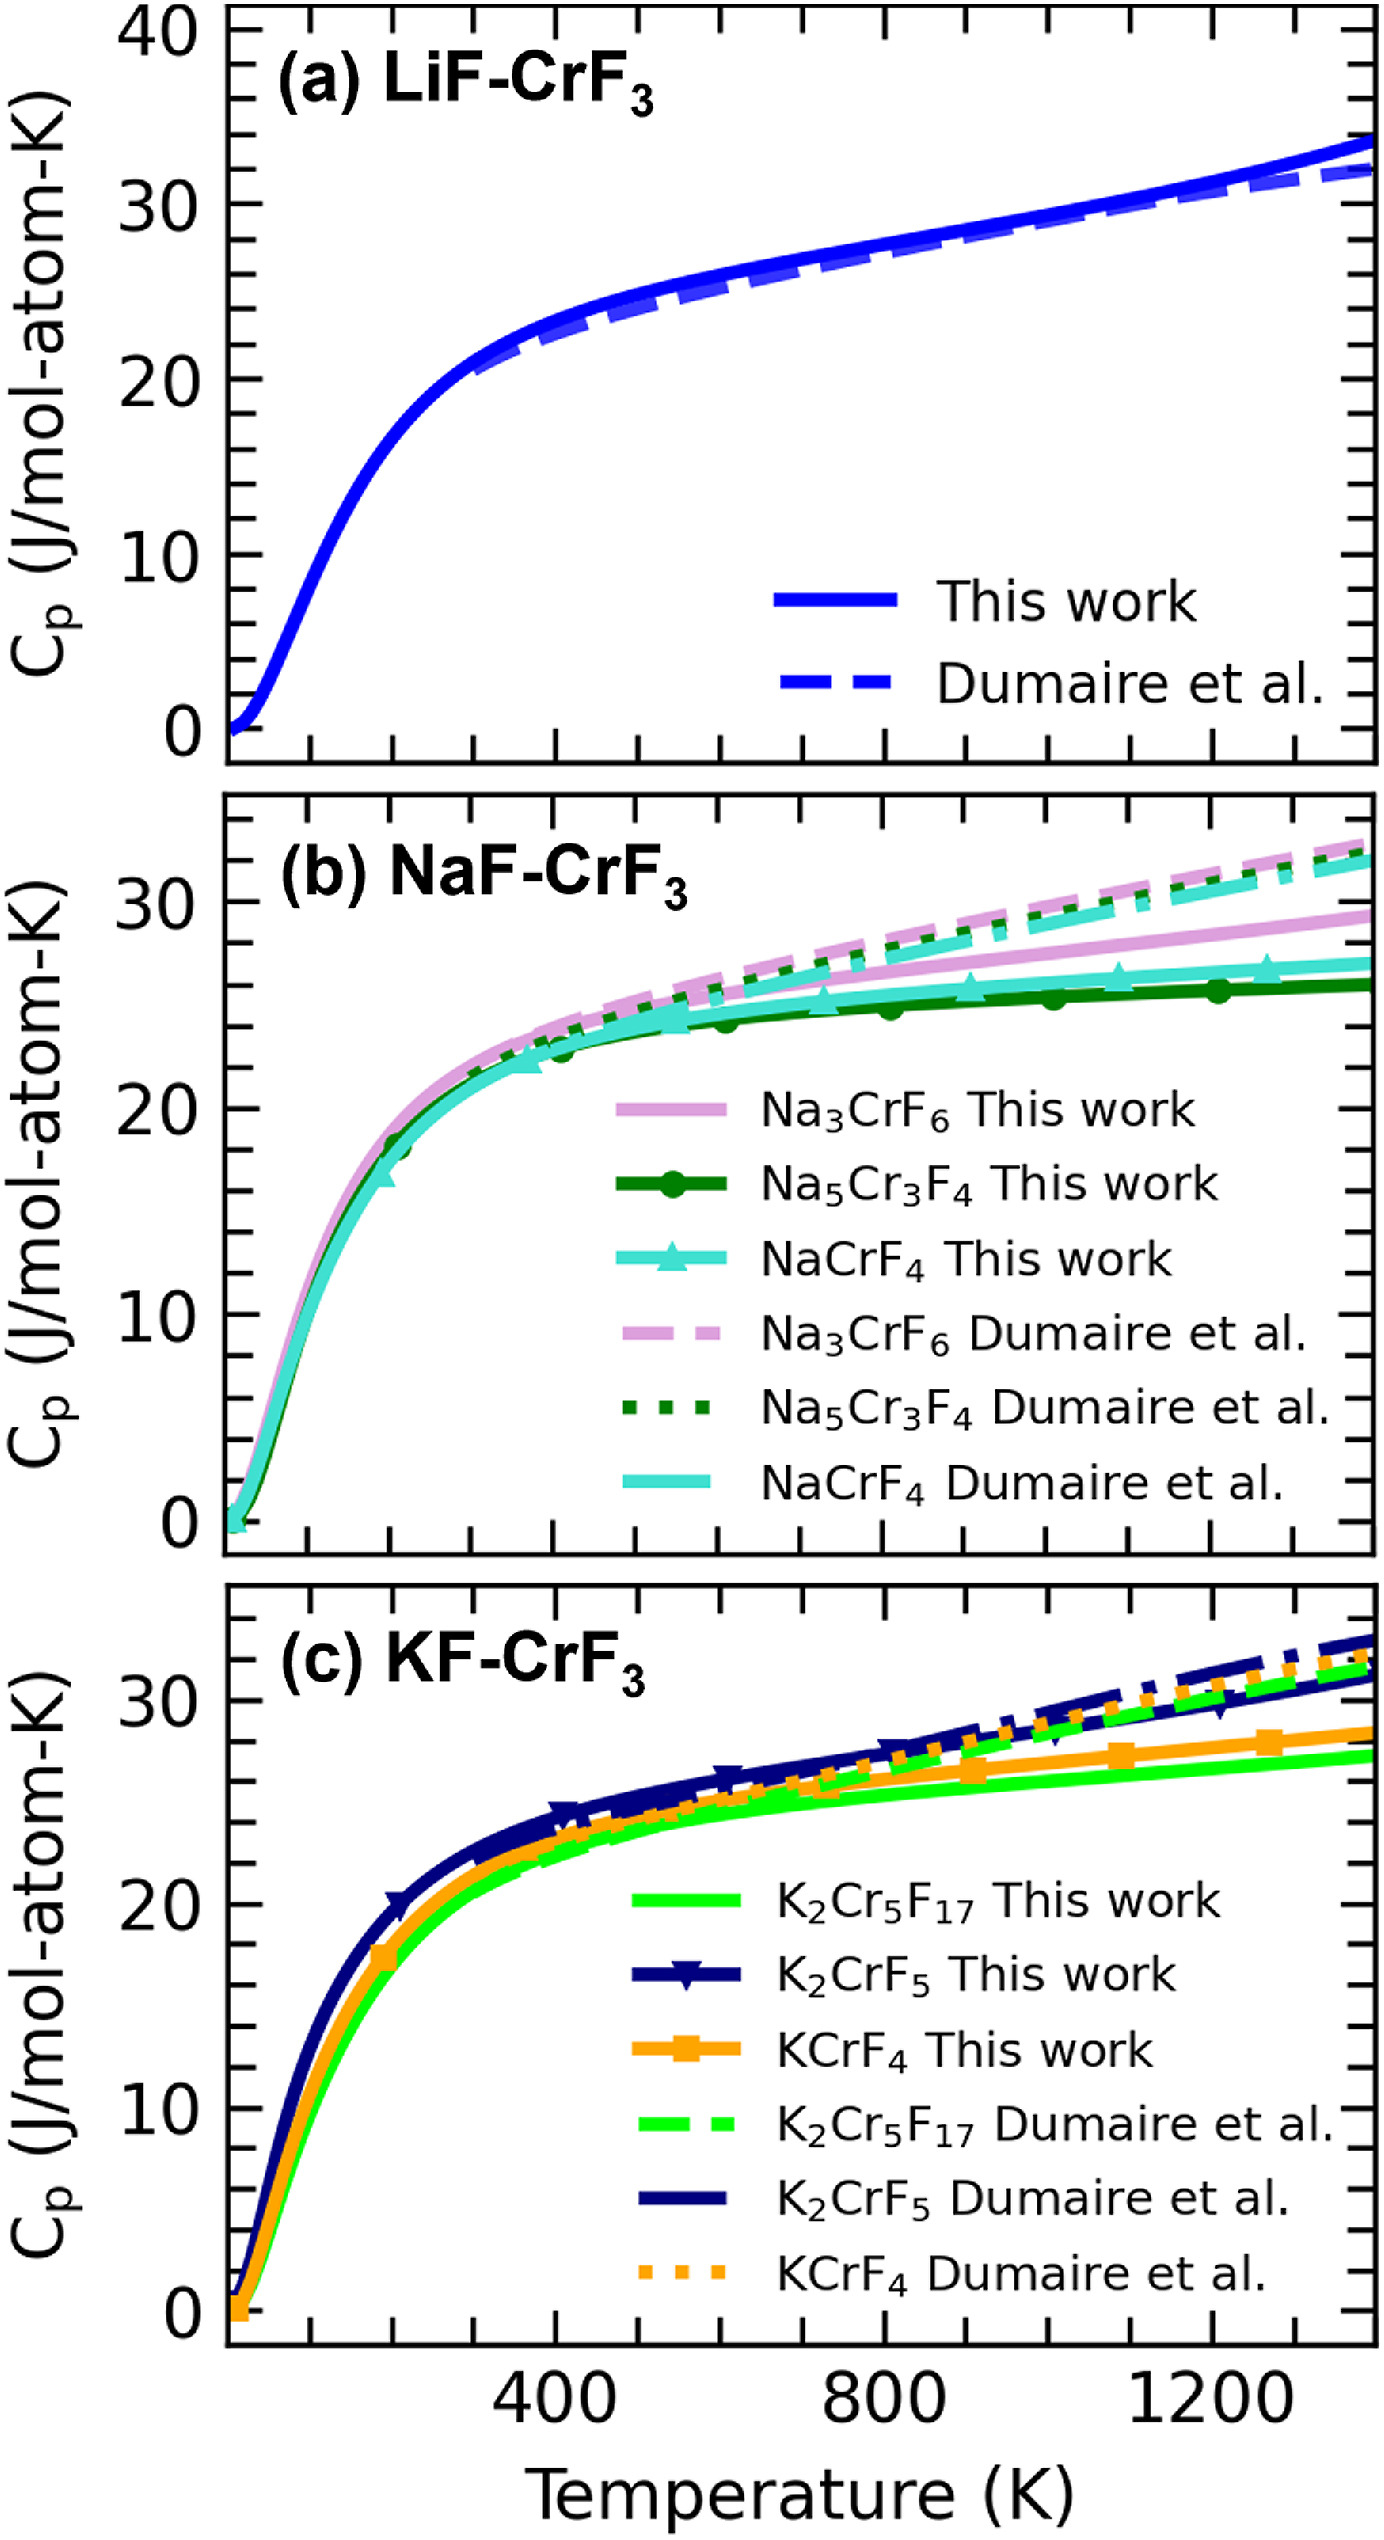
\includegraphics[width=0.45\linewidth]{moltensalts/Moltensalts-FLiNaKCr-DFTcompounds.jpg}
    \caption{Predicted heat capacities of ternary compounds in the (a) LiF–CrF$_3$, (b) NaF–CrF$_3$, and (c) KF-CrF$_3$ systems by DFT-based QHA via phonon calculations (solid lines) compared with the Dumaire et al. \cite{dumaire2021thermodynamic}'s work (dashed lines). The QHA results are implemented in the present modeling work for ternary compounds.}
    \label{ms:fig:FLiNaKCr-DFTcompounds}
\end{figure}



\subsection{Thermodynamic modeling of the (LiF, NaF, KF, CrF$_2$)-CrF$_3$ system} \label{moltensalts:ssec:FLiNaKCrmodeling}

Figure \ref{ms:fig:FLiNaKCr-Phasediagram} shows the phase diagrams of the (LiF, NaF, KF, and CrF$_2$)-CrF$_3$ systems calculated from present models and compared with experimental data by De Kozak \cite{de1975systeme, DeKozak1969} and Sturm \cite{sturm1962phase}. The present CALPHAD modeling shows a good agreement regarding phase boundaries with experimental data. The presently modeled parameters for liquid and the complete thermodynamic database can be found in the Supplementary XML file \cite{gong2024revisiting}. Details of the invariant reactions and the congruent melting temperature calculated from the present modeling work compared to experiments \cite{de1975systeme, DeKozak1969, sturm1962phase} and ML predictions using Hong et al.’s model \cite{hong2022melting} are listed in Table \ref{ms:tab:FLiNaK-Cr-inv} with discussion below. 

\begin{figure}[H]
    \centering
    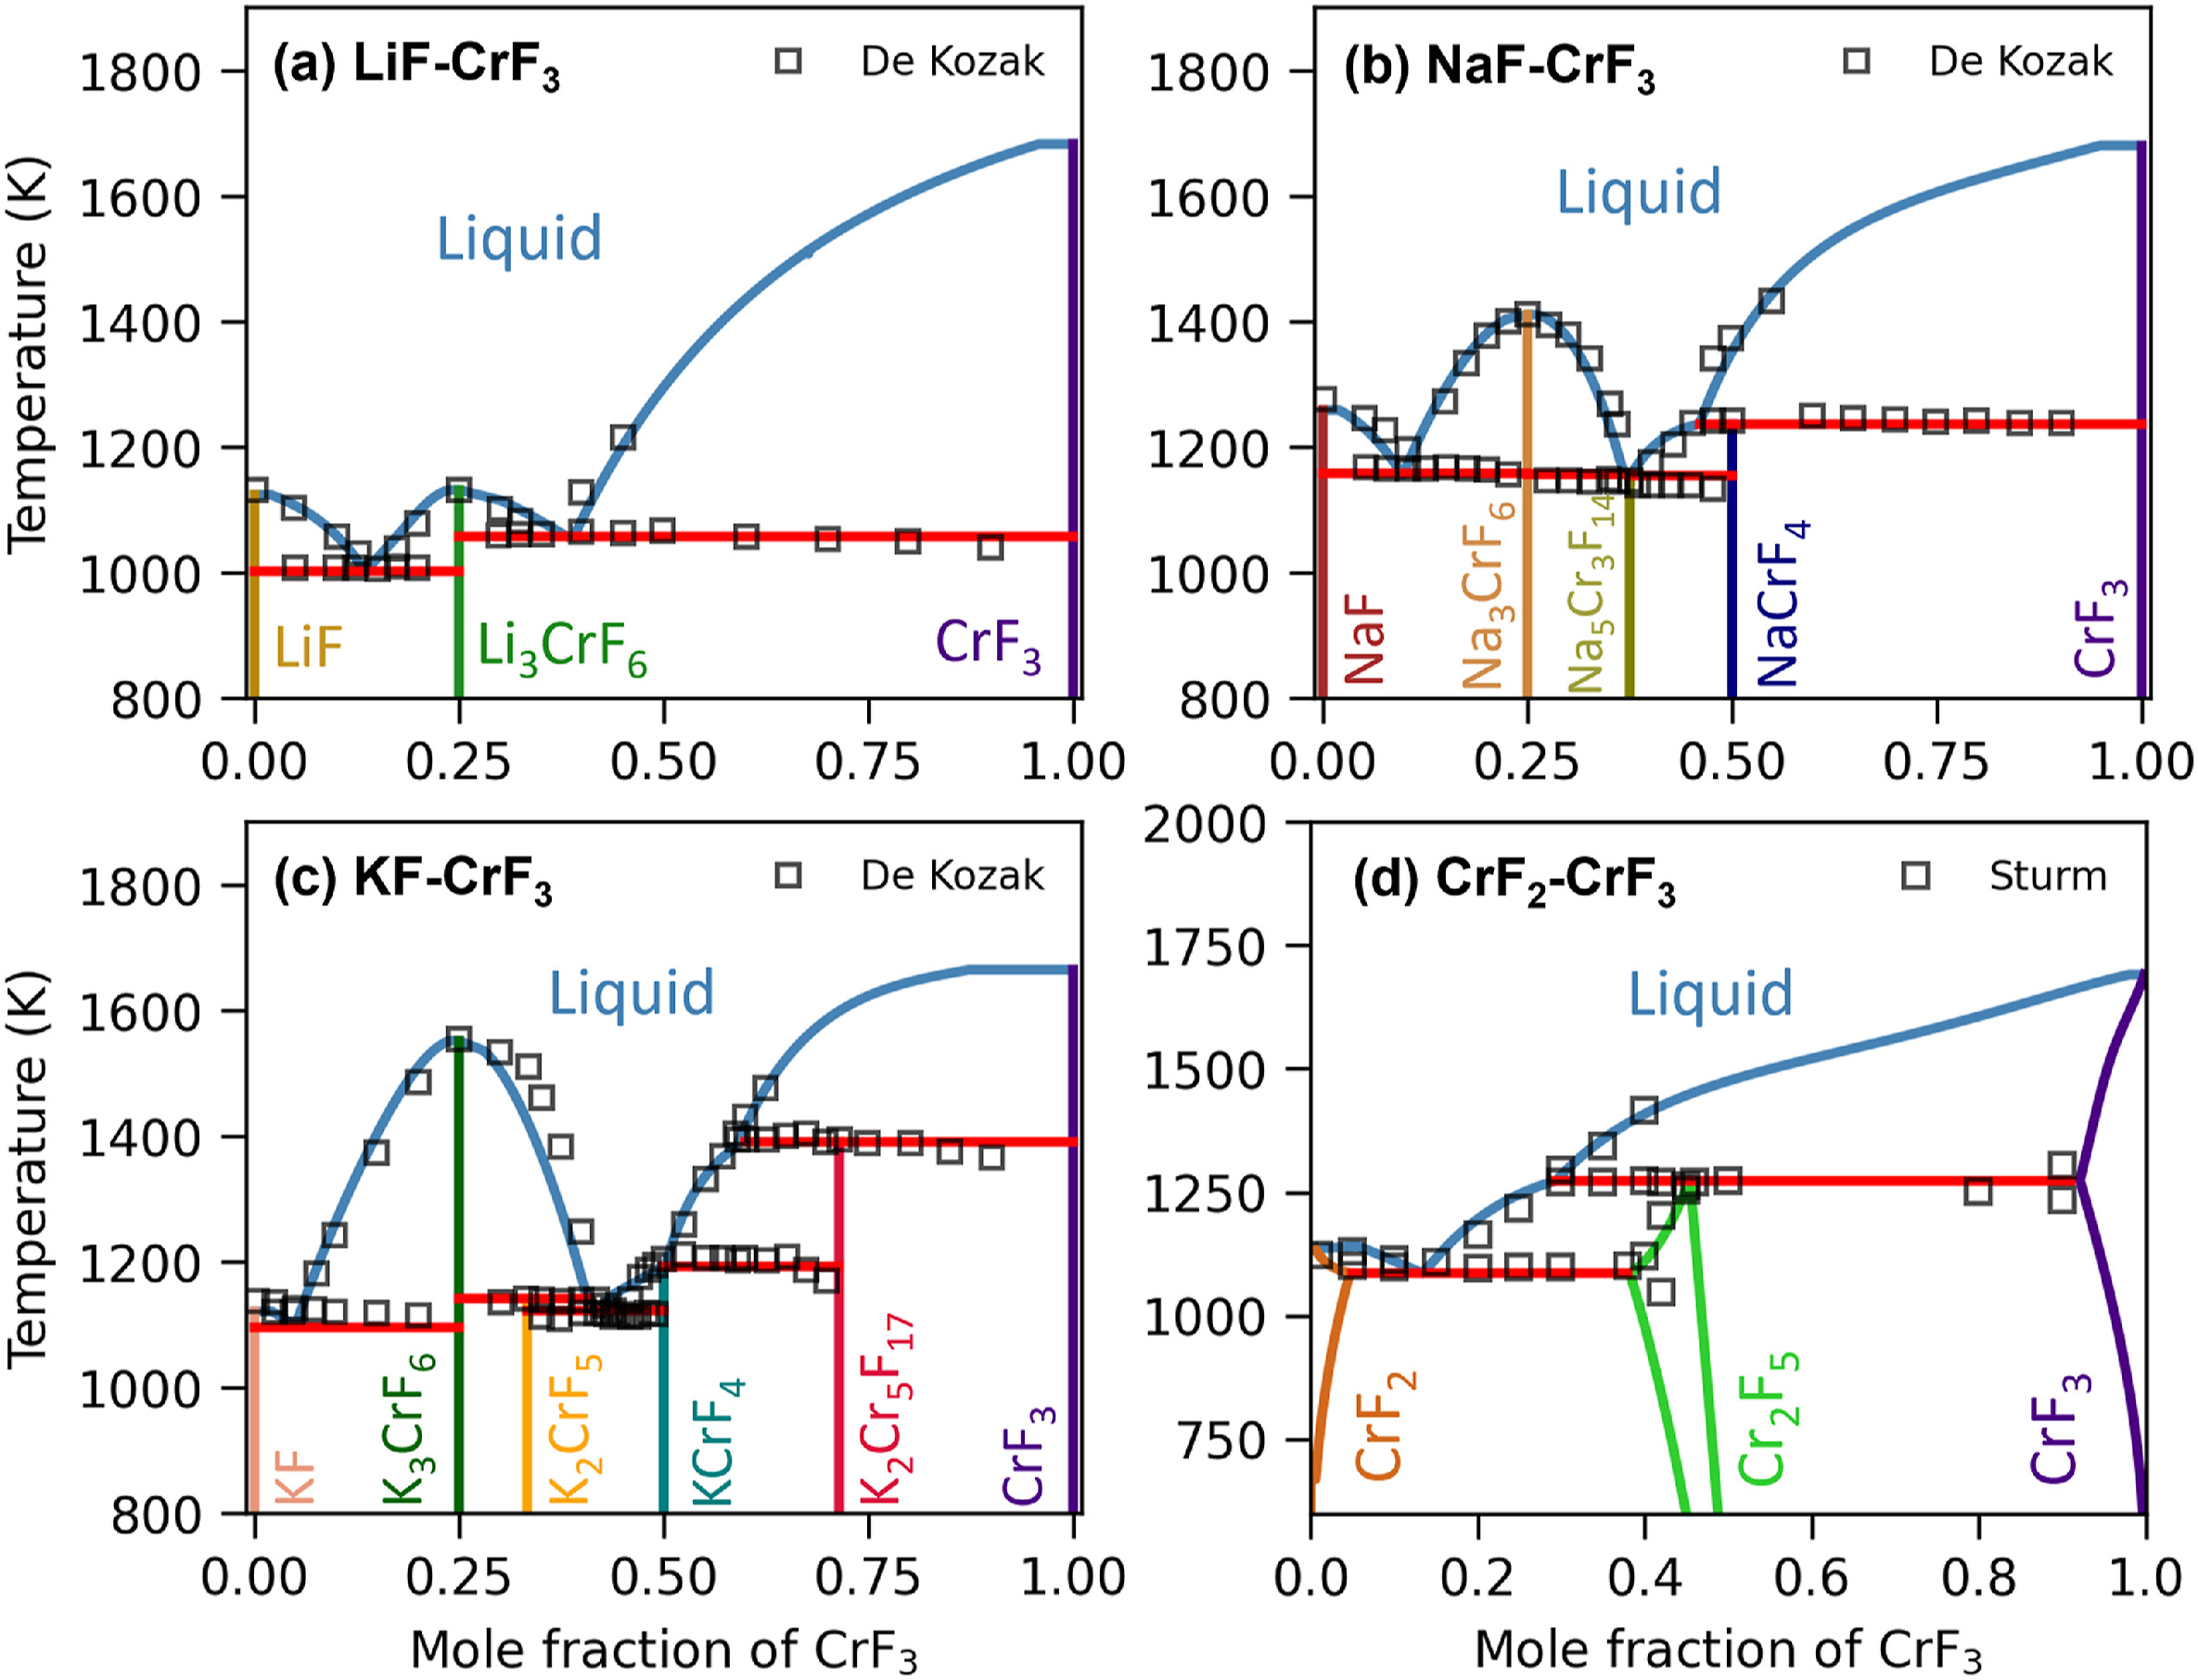
\includegraphics[width=1\linewidth]{moltensalts/Moltensalts-FLiNaKCr-Phasediagram.jpg}
    \caption{Predicted phase diagrams of the (a) LiF–CrF$_3$, (b) NaF–CrF$_3$, (c) KF-CrF$_3$, and (d) CrF$_2$–CrF$_3$ systems by the present CALPHAD modeling in comparison with experimental data \cite{de1975systeme, DeKozak1969, sturm1962phase}.}
    \label{ms:fig:FLiNaKCr-Phasediagram}
\end{figure}
\newpage
\begingroup
\renewcommand\arraystretch{0.8}
\begin{longtable}[H]{>{\raggedright\arraybackslash}m{2cm}>{\raggedright\arraybackslash}m{6cm}>{\raggedright\arraybackslash}m{1.5cm}>{\raggedright\arraybackslash}m{3cm}>{\raggedright\arraybackslash}m{3.5cm}}
    \caption{Predicted invariant equilibria in the AF-CrF$_3$ (A=Li, Na, K) systems by the present CALPHAD modeling, compared with experimental data from De Kozak \cite{DeKozak1969} and Sturm \cite{sturm1962phase} (marked with *), and other modeling works \cite{yin2014thermodynamic, yin2015thermodynamic, yin2018thermodynamic, dumaire2021thermodynamic}.}\\
    \hline
    \textbf{Reaction}&&\textbf{$x$(CrF$_3$)}&\textbf{Temperature (K)}&\textbf{Source}\\
    \hline
    Eutectic&Liquid$\leftrightarrow$LiF+Li$_3$CrF$_6$&0.135&1002&This work\\
    &&0.150&1003&De Kozak \cite{DeKozak1969}$^*$\\
    &&0.136&1008&Dumaire et al. \cite{dumaire2021thermodynamic}\\
    &&0.148&1003&Yin et al. \cite{yin2014thermodynamic}\\
    Congruent melting&Liquid$\leftrightarrow$Li$_3$CrF$_6$&0.25&1131&This work\\
    &&0.25&1129&De Kozak \cite{DeKozak1969}$^*$\\
    &&0.25&1114&Hong et al. \cite{hong2022melting}\\
    &&0.25&1111&Dumaire et al. \cite{dumaire2021thermodynamic}\\
    &&0.25&1125&Yin et al. \cite{yin2014thermodynamic}\\
    Eutectic&Liquid$\leftrightarrow$CrF$_3$+Li$_3$CrF$_6$&0.382&1056&This work\\
    &&0.350&1059&De Kozak \cite{DeKozak1969}$^*$\\
    &&0.363&1062&Dumaire et al. \cite{dumaire2021thermodynamic}\\
    &&0.354&1058&Yin et al. \cite{yin2014thermodynamic}\\
    Eutectic&Liquid$\leftrightarrow$NaF+Na$_3$CrF$_6$&0.098&1155&This work\\
    &&0.123&1166&De Kozak \cite{DeKozak1969}$^*$\\
    &&0.106&1175&Dumaire et al. \cite{dumaire2021thermodynamic}\\
    &&0.114&1162&Yin et al. \cite{yin2018thermodynamic}\\
    Congruent melting&Liquid$\leftrightarrow$Na$_3$CrF$_6$&0.25&1410&This work\\
    &&0.25&1413&De Kozak \cite{DeKozak1969}$^*$\\
    &&0.25&1404&Hong et al. \cite{hong2022melting}\\
    &&0.25&1385&Dumaire et al. \cite{dumaire2021thermodynamic}\\
    &&0.25&1416&Yin et al. \cite{yin2018thermodynamic}\\
    Eutectic&Liquid$\leftrightarrow$Na$_5$Cr$_3$F$_{14}$+Na$_3$CrF$_6$&0.368&1155&This work\\
    &&0.371&1145&Dumaire et al. \cite{dumaire2021thermodynamic}\\
    &&0.367&1142&Yin et al. \cite{yin2018thermodynamic}\\
    Eutectic&Liquid$\leftrightarrow$Na$_5$Cr$_3$F$_{14}$+NaCrF$_4$&0.377&1154&This work\\
    &&0.381&1144&Dumaire et al. \cite{dumaire2021thermodynamic}\\
    &&0.383&1141&Yin et al. \cite{yin2018thermodynamic}\\
    Peritectic&Liquid+CrF$_3$$\leftrightarrow$NaCrF$_4$&0.5&1235&This work\\
    &&0.5&1234&De Kozak \cite{DeKozak1969}$^*$\\
    &&0.5&1232&Dumaire et al. \cite{dumaire2021thermodynamic}\\
    &&0.5&1239&Yin et al. \cite{yin2018thermodynamic}\\
    Eutectic&Liquid$\leftrightarrow$KF+K$_3$CrF$_6$&0.050&1096&This work\\
    &&0.048&1115&De Kozak \cite{DeKozak1969}$^*$\\
    &&0.041&1108&Dumaire et al. \cite{dumaire2021thermodynamic}\\
    &&0.045&1113&Yin et al. \cite{yin2018thermodynamic}\\ 
    Congruent melting&Liquid$\leftrightarrow$K$_3$CrF$_6$&0.25&1551&This work\\
    &&0.25&1553&De Kozak \cite{DeKozak1969}$^*$\\
    &&0.25&1520&Hong et al. \cite{hong2022melting}\\
    &&0.25&1553&Dumaire et al. \cite{dumaire2021thermodynamic}\\
    &&0.25&1548&Yin et al. \cite{yin2015thermodynamic}\\ 
    Peritectic&Liquid+K$_3$CrF$_6$$\leftrightarrow$K$_2$CrF$_5$&0.333&1141&This work\\
    &&0.333&1133&De Kozak \cite{DeKozak1969}$^*$\\
    &&0.333&1130&Dumaire et al. \cite{dumaire2021thermodynamic}\\
    &&0.333&1135&Yin et al. \cite{yin2015thermodynamic}\\  
    Eutectic&Liquid$\leftrightarrow$KCrF$_4$+K$_2$CrF$_5$&0.420&1120&This work\\
    &&0.45&1112&De Kozak \cite{DeKozak1969}$^*$\\
    &&0.432&1112&Dumaire et al. \cite{dumaire2021thermodynamic}\\
    &&0.426&1107&Yin et al. \cite{yin2015thermodynamic}\\  
    Peritectic&Liquid+K$_2$Cr$_5$F$_{17}$$\leftrightarrow$KCrF$_4$&0.5&1192&This work\\
    &&0.5&1200&De Kozak \cite{DeKozak1969}$^*$\\
    &&0.5&1191&Dumaire et al.  \cite{dumaire2021thermodynamic}\\
    &&0.5&1195&Yin et al. \cite{yin2015thermodynamic}\\ 
    Peritectic&Liquid+CrF$_3$$\leftrightarrow$K$_2$Cr$_5$F$_{17}$&0.714&1390&This work\\
    &&0.714&1390&De Kozak \cite{DeKozak1969}$^*$\\
    &&0.714&1390&Dumaire et al. \cite{dumaire2021thermodynamic}\\
    &&0.714&1388&Yin et al. \cite{yin2015thermodynamic}\\ 
    Eutectic&Liquid$\leftrightarrow$CrF$_2$+Cr$_2$F$_5$&0.134&1086&This work\\
    &&0.14&1103&Sturm \cite{sturm1962phase}$^*$\\
    &&0.115&1104&Dumaire et al. \cite{dumaire2021thermodynamic}\\
    Peritectic&Liquid+CrF$_3$$\leftrightarrow$Cr$_2$F$_5$&0.293&1273&This work\\
    &&0.29&1272&Sturm \cite{sturm1962phase}$^*$\\
    &&0.28&1271&Dumaire et al. \cite{dumaire2021thermodynamic}\\
    \hline
    \label{ms:tab:FLiNaK-Cr-inv}
\end{longtable}
\endgroup

In the LiF-CrF$_3$ system, the present prediction of the eutectic reaction Liquid $\leftrightarrow$ CrF$_3$ + Li$_3$CrF$_6$ at T = 1056 K matches closely with experimental values of T = 1059 K \cite{DeKozak1969}. There is a minor difference of 1 K observed for Liquid $\leftrightarrow$ LiF + Li$_3$CrF$_6$, with the present modeling predicts an eutectic temperature of 1002 K compared to 1003 K reported by De Kozak \cite{DeKozak1969}. This presents an improvement over the 1008 K predicted by Dumaire et al. \cite{dumaire2021thermodynamic}’s modeling. The present prediction of the congruent melting temperature of 1131 K is 2 K higher than the experimental value of 1129 K reported by De Kozak \cite{DeKozak1969}, significantly improved from the prediction of 1111 K by Dumaire et al. \cite{dumaire2021thermodynamic}. 

In the NaF-CrF$_3$ system, the present modeling gives good predictions of eutectic and peritectic temperatures compared with experiments \cite{DeKozak1969}. The difference of 1 K is observed for Liquid + CrF$_3$ $\leftrightarrow$ NaCrF$_4$ (1235 K from the present work and 1234 K by De Kozak \cite{DeKozak1969}). The eutectic composition for the reaction Liquid $\leftrightarrow$ NaF + Na$_3$CrF$_6$ is $x$(CrF$_3$) = 0.098, which is around 0.025 away from the experimental value $x$(CrF$_3$) = 0.123 \cite{DeKozak1969}. The eutectic temperature for this reaction by the present modeling is 1155 K, in comparison to the experimental value of 1166 K by De Kozak \cite{DeKozak1969}. The present congruent melting temperature of Na$_3$CrF$_6$ is predicted at 1410 K, improving from the predicted 1385 K by Dumaire et al. \cite{dumaire2021thermodynamic} but slightly lower than the experimental value of 1413 K \cite{DeKozak1969}. For the two eutectic reactions without experimental data, i.e., Liquid $\leftrightarrow$ Na$_5$Cr$_3$F$_{14}$ + Na$_3$CrF$_6$ and Liquid $\leftrightarrow$ Na$_5$Cr$_3$F$_{14}$ + NaCrF$_4$, the present modeling provides similar predictions ($x$(CrF$_3$) = 0.368, T = 1155 K; $x$(CrF$_3$) = 0.377, T = 1154 K respectively) compared to those modeled by Dumaire et al. \cite{dumaire2021thermodynamic} ($x$(CrF$_3$) = 0.371, T = 1145 K; $x$(CrF$_3$) = 0.381, T = 1144 K, respectively). 

In the KF-CrF$_3$ system, the present modeling work predicts the congruent melting of K$_3$CrF$_6$ at 1551 K, which is in good agreement with the experimental value of 1553 K \cite{DeKozak1969}. For the eutectic reaction, Liquid $\leftrightarrow$ KCrF$_4$ + K$_2$CrF$_5$, the present modeling predicts $x$(CrF$_3$) = 0.42 and T = 1120 K, whereas the values are $x$(CrF$_3$) = 0.45 and T = 1112 K modeled by De Kozak \cite{DeKozak1969}. The present modeling predicts a eutectic temperature of Liquid $\leftrightarrow$ KF + K$_3$CrF$_6$ at 1096 K, slightly lower than the experimental value of 1115 K by De Kozak \cite{DeKozak1969}. For the three peritectic reactions in the KF-CrF$_3$ system, the present modeling work predicts 1141 K for Liquid + K$_3$CrF$_6$ $\leftrightarrow$ K$_2$CrF$_5$, 1192 K for Liquid + K$_2$Cr$_5$F$_{17}$ $\leftrightarrow$ KCrF$_4$, and 1390 K for Liquid + CrF$_3$ $\leftrightarrow$ K$_2$Cr$_5$F$_{17}$. These temperatures are comparable to 1133 K, 1200 K, and 1390 K, respectively, as measured by De Kozak \cite{DeKozak1969}, showing an MAE of 5.33 K.

In the CrF$_2$-CrF$_3$ system, the present modeling work improves the predicted invariant compositions. For the eutectic reaction Liquid$\leftrightarrow$CrF$_2$+Cr$_2$F$_5$, the present work predicts the eutectic point at $x$(CrF$_3$) = 0.134. This value is higher than $x$(CrF$_3$) = 0.115 by Dumaire et al. \cite{dumaire2021thermodynamic} but aligns more closely with the experimental value $x$(CrF$_3$) = 0.14 by Sturm \cite{sturm1962phase}. The eutectic temperature for this reaction is 1086 K predicted by the present modeling, demonstrating a slightly lower value of 17 K than the measured 1103 K by Sturm \cite{sturm1962phase}. For the peritectic reaction Liquid + CrF$_3$ $\leftrightarrow$ Cr$_2$F$_5$, the present work predicts $x$(CrF$_3$) = 0.293 compared to measured $x$(CrF$_3$) = 0.29 by Sturm \cite{sturm1962phase}. The present invariant temperature is predicted at 1273 K, which remains close to the experimental 1272 K by Sturm \cite{sturm1962phase}. In the present work, the single-phase region of the Cr$_2$F$_5$ solid solution phase ranges from $x$(CrF$_3$) = 0.38 to $x$(CrF$_3$) = 0.46. This range aligns well with the suggested values of $x$(CrF$_3$) from 0.40 to 0.45 by Sturm \cite{sturm1962phase}. Overall, by incorporating thermodynamic data of compounds by the present DFT calculations, the present modeling work yields improved predictions of phase diagrams.

The present CALPHAD modeling work implements the mixing enthalpy of liquid at 1700 K, which was obtained by the present AIMD simulations as described in Section \ref{moltensalts:ssec:FLiNaKCrmodel}. Note that the mixing enthalpy values from AIMD simulations can be found in the Supplementary JSON files \cite{gong2024revisiting}. Figure \ref{ms:fig:FLiNaKCr-Hmix} shows the mixing enthalpy of liquid at 1700 K by AIMD at different compositions compared to the present modeling results and results by Dumaire et al. \cite{dumaire2021thermodynamic}. It clearly shows that the mixing enthalpy of liquid (dot-dashed lines) by Dumaire et al.’s modeling \cite{dumaire2021thermodynamic} is much less negative compared to the present AIMD calculations. For example, in the LiF-CrF$_3$ system at $x$(CrF$_3$) = 0.2, AIMD predicts the mixing enthalpy of $-20.60$ kJ/mol-atom at 1700 K, while Dumaire et al’s modeling \cite{dumaire2021thermodynamic} shows $-12.65$ kJ/mol-atom, representing a 39\% higher value. Using the present AIMD data of liquid for modeling, the present modeling work (solid lines) shows a great improvement. The present modeling work improves the prediction to $-18.99$ kJ/mol-atom at $x$(CrF$_3$) = 0.2 for the LiF-CrF$_3$ system. The differences between the AIMD results and Dumaire et al.’s work \cite{dumaire2021thermodynamic} are more pronounced in the NaF-CrF$_3$ and KF-CrF$_3$ systems. In the NaF-CrF$_3$ system, at $x$(CrF$_3$) = 0.333 (a composition region near the lowest mixing enthalpy), Dumaire et al.’s modeling \cite{dumaire2021thermodynamic} shows the mixing enthalpy of $-25.45$ kJ/mol-atom, while our modeling predicts $-49.96$ kJ/mol-atom. At the same condition, AIMD gives the mixing enthalpy of $-47.37$ kJ/mol-atom, which is about 22 kJ/mol-atom lower than Dumaire et al.’s results \cite{dumaire2021thermodynamic}. In the KF-CrF$_3$ system at $x$(CrF$_3$) = 0.333, Dumaire et al. \cite{dumaire2021thermodynamic} predicts $-30.58$ kJ/mol-atom, significantly higher than $-50.20$ kJ/mol-atom by AIMD. The present modeling predicts $-53.70$ kJ/mol-atom, reducing the difference from the above-mentioned 39\% to the present 7\%. It highlights that the present AIMD simulations enhance the reliability of the present modeling in describing liquid compared to the previous work \cite{dumaire2021thermodynamic}. The mixing enthalpy (dotted lines) modeling by Yin et al. \cite{yin2018thermodynamic} in the NaF-CrF$_3$ and KF-CrF$_3$ systems agree well with the results of the present modeling. Near the low mixing enthalpy region $x$(CrF$_3$) = 0.333 in the NaF-CrF$_3$ system, Yin et al. \cite{yin2018thermodynamic} suggest the mixing enthalpy of $-40.54$ kJ/atom, which is 19\% higher than $-49.96$ kJ/atom from the present work. Note that Yin et al. \cite{yin2018thermodynamic} used an empirical model proposed by Robelin and Chartrand \cite{robelin2011thermodynamic} to estimate the mixing enthalpy in liquid. Overall, the present modeling work has improved the predictions of liquid than the modeling works by Dumaire et al. \cite{dumaire2021thermodynamic} and Yin et al. \cite{yin2018thermodynamic}. 

\begin{figure}[H]
    \centering
    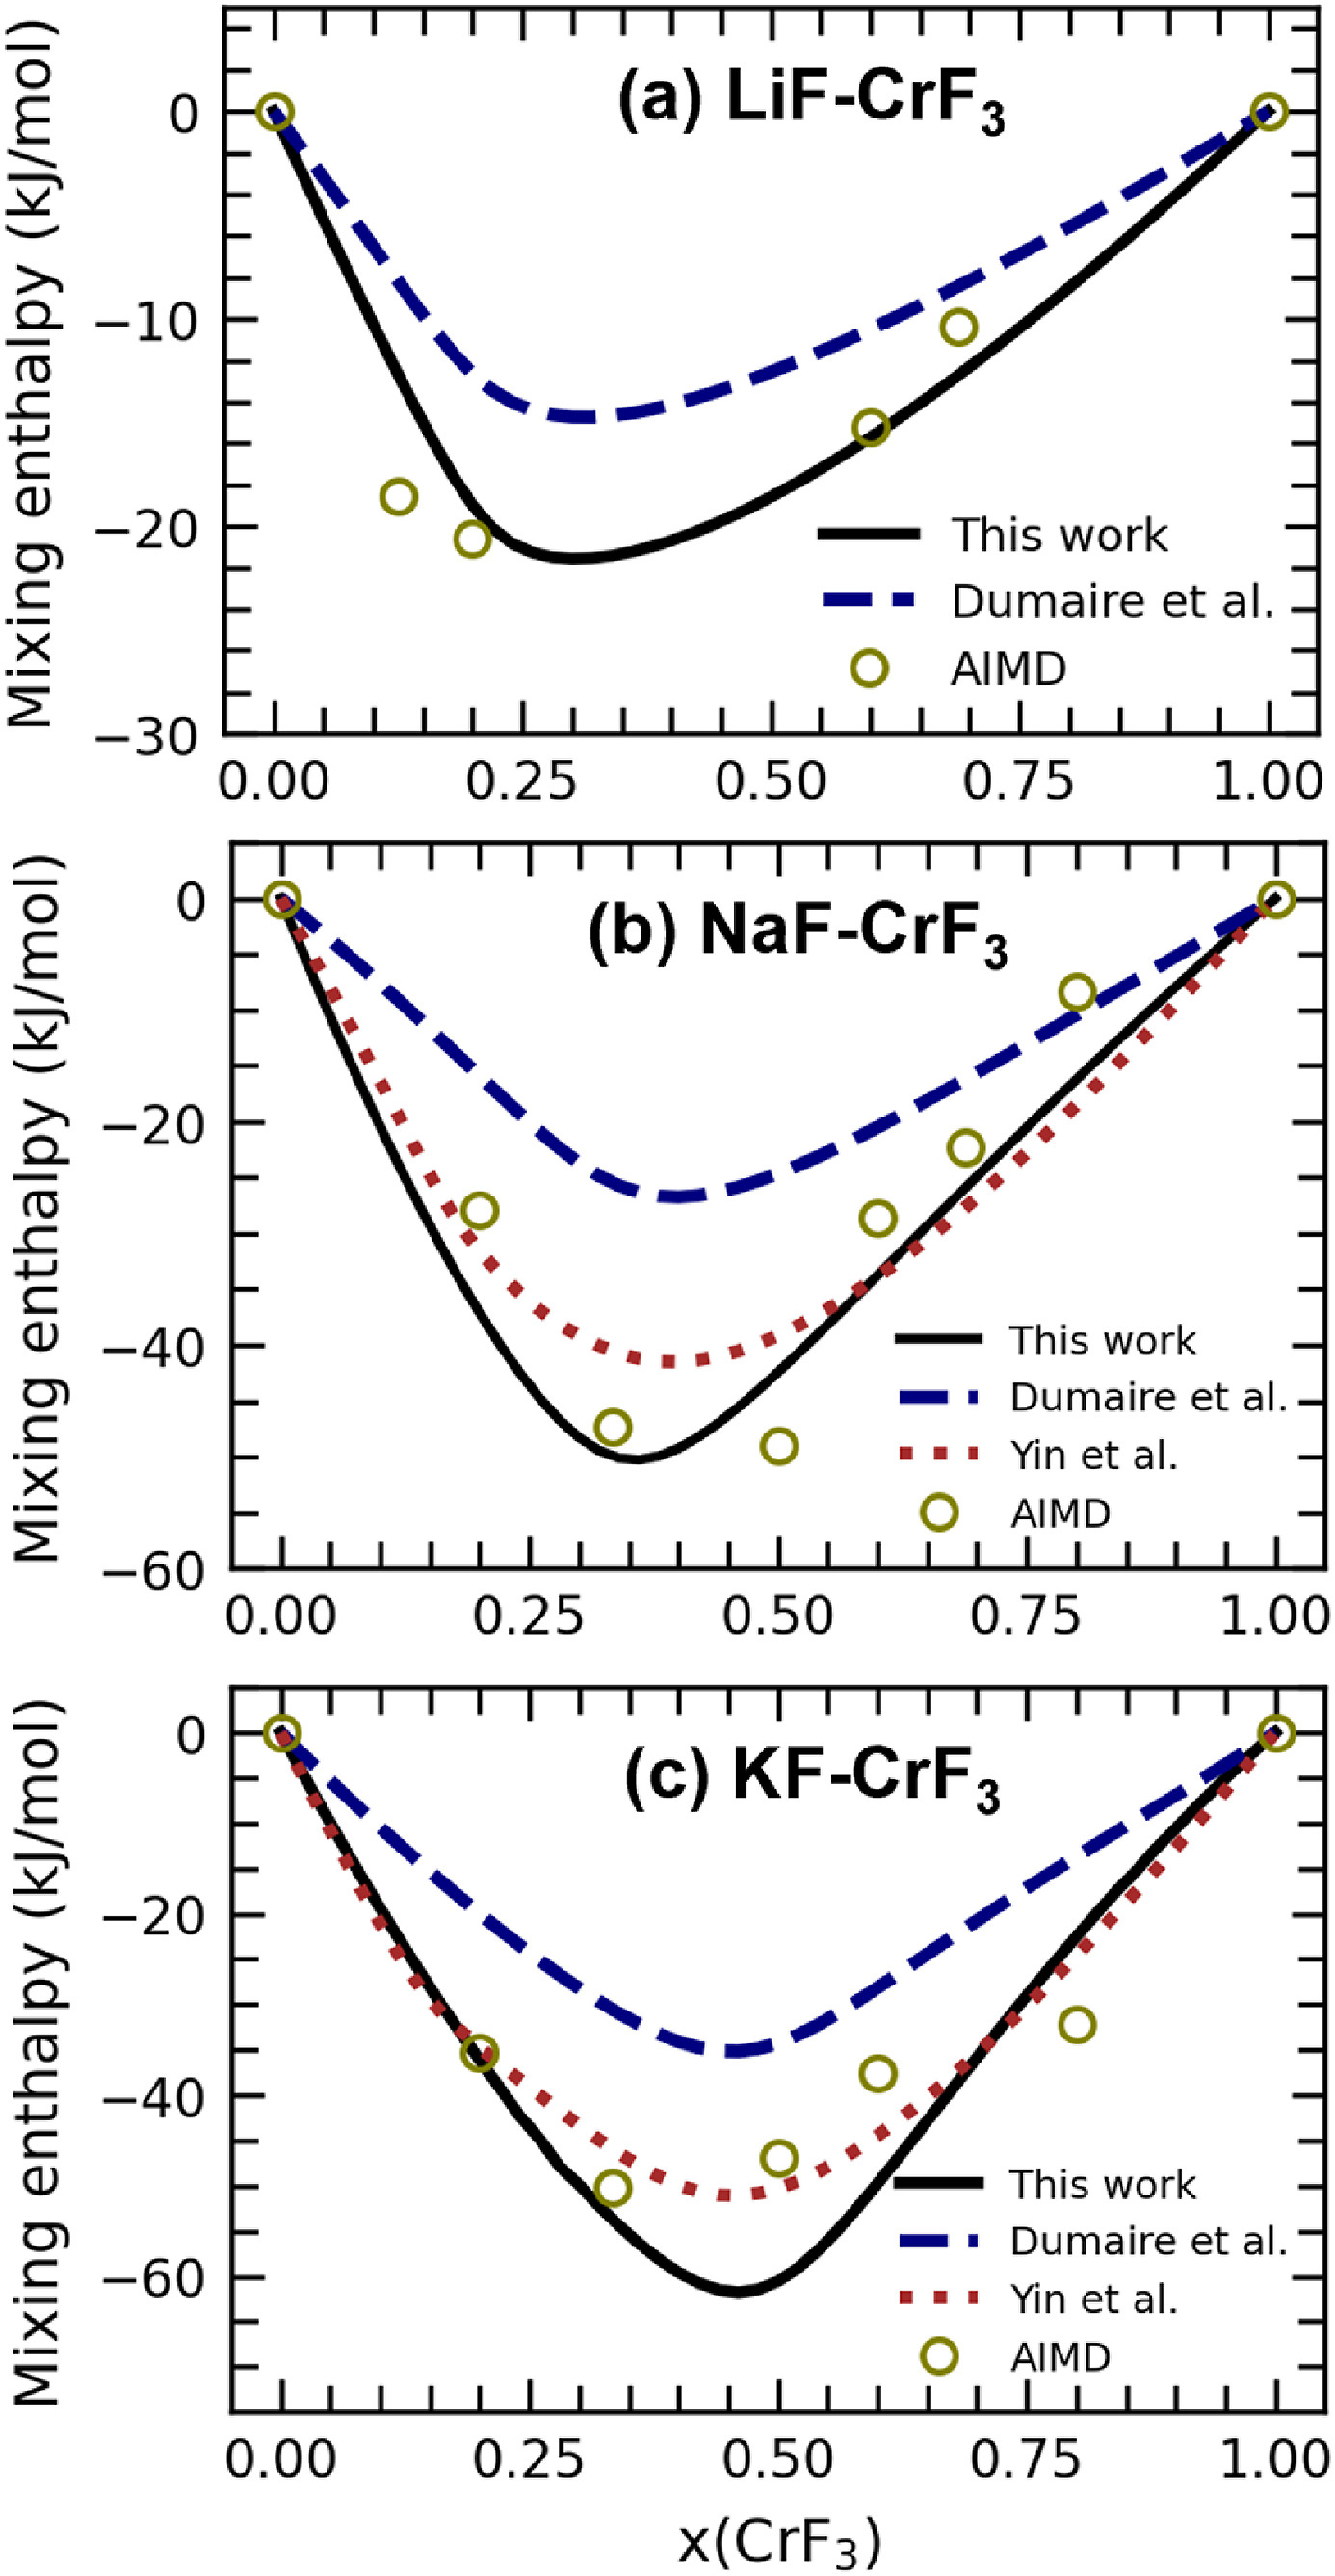
\includegraphics[width=0.45\linewidth]{moltensalts/Moltensalts-FLiNaKCr-Hmix.jpg}
    \caption{Predicted mixing enthalpy of liquid at 1700 K in (a) LiF-CrF$_3$, (b) NaF-CrF$_3$, and (c) KF-CrF$_3$ by the present CALPHAD modeling work (black solid lines), compared with the present AIMD results (circles) and modeling results by Dumaire et al. (blue dashed lines) \cite{dumaire2021thermodynamic} and Yin et al. (brown dotted lines) \cite{yin2018thermodynamic}.}
    \label{ms:fig:FLiNaKCr-Hmix}
\end{figure}

\begin{figure}[H]
    \centering
    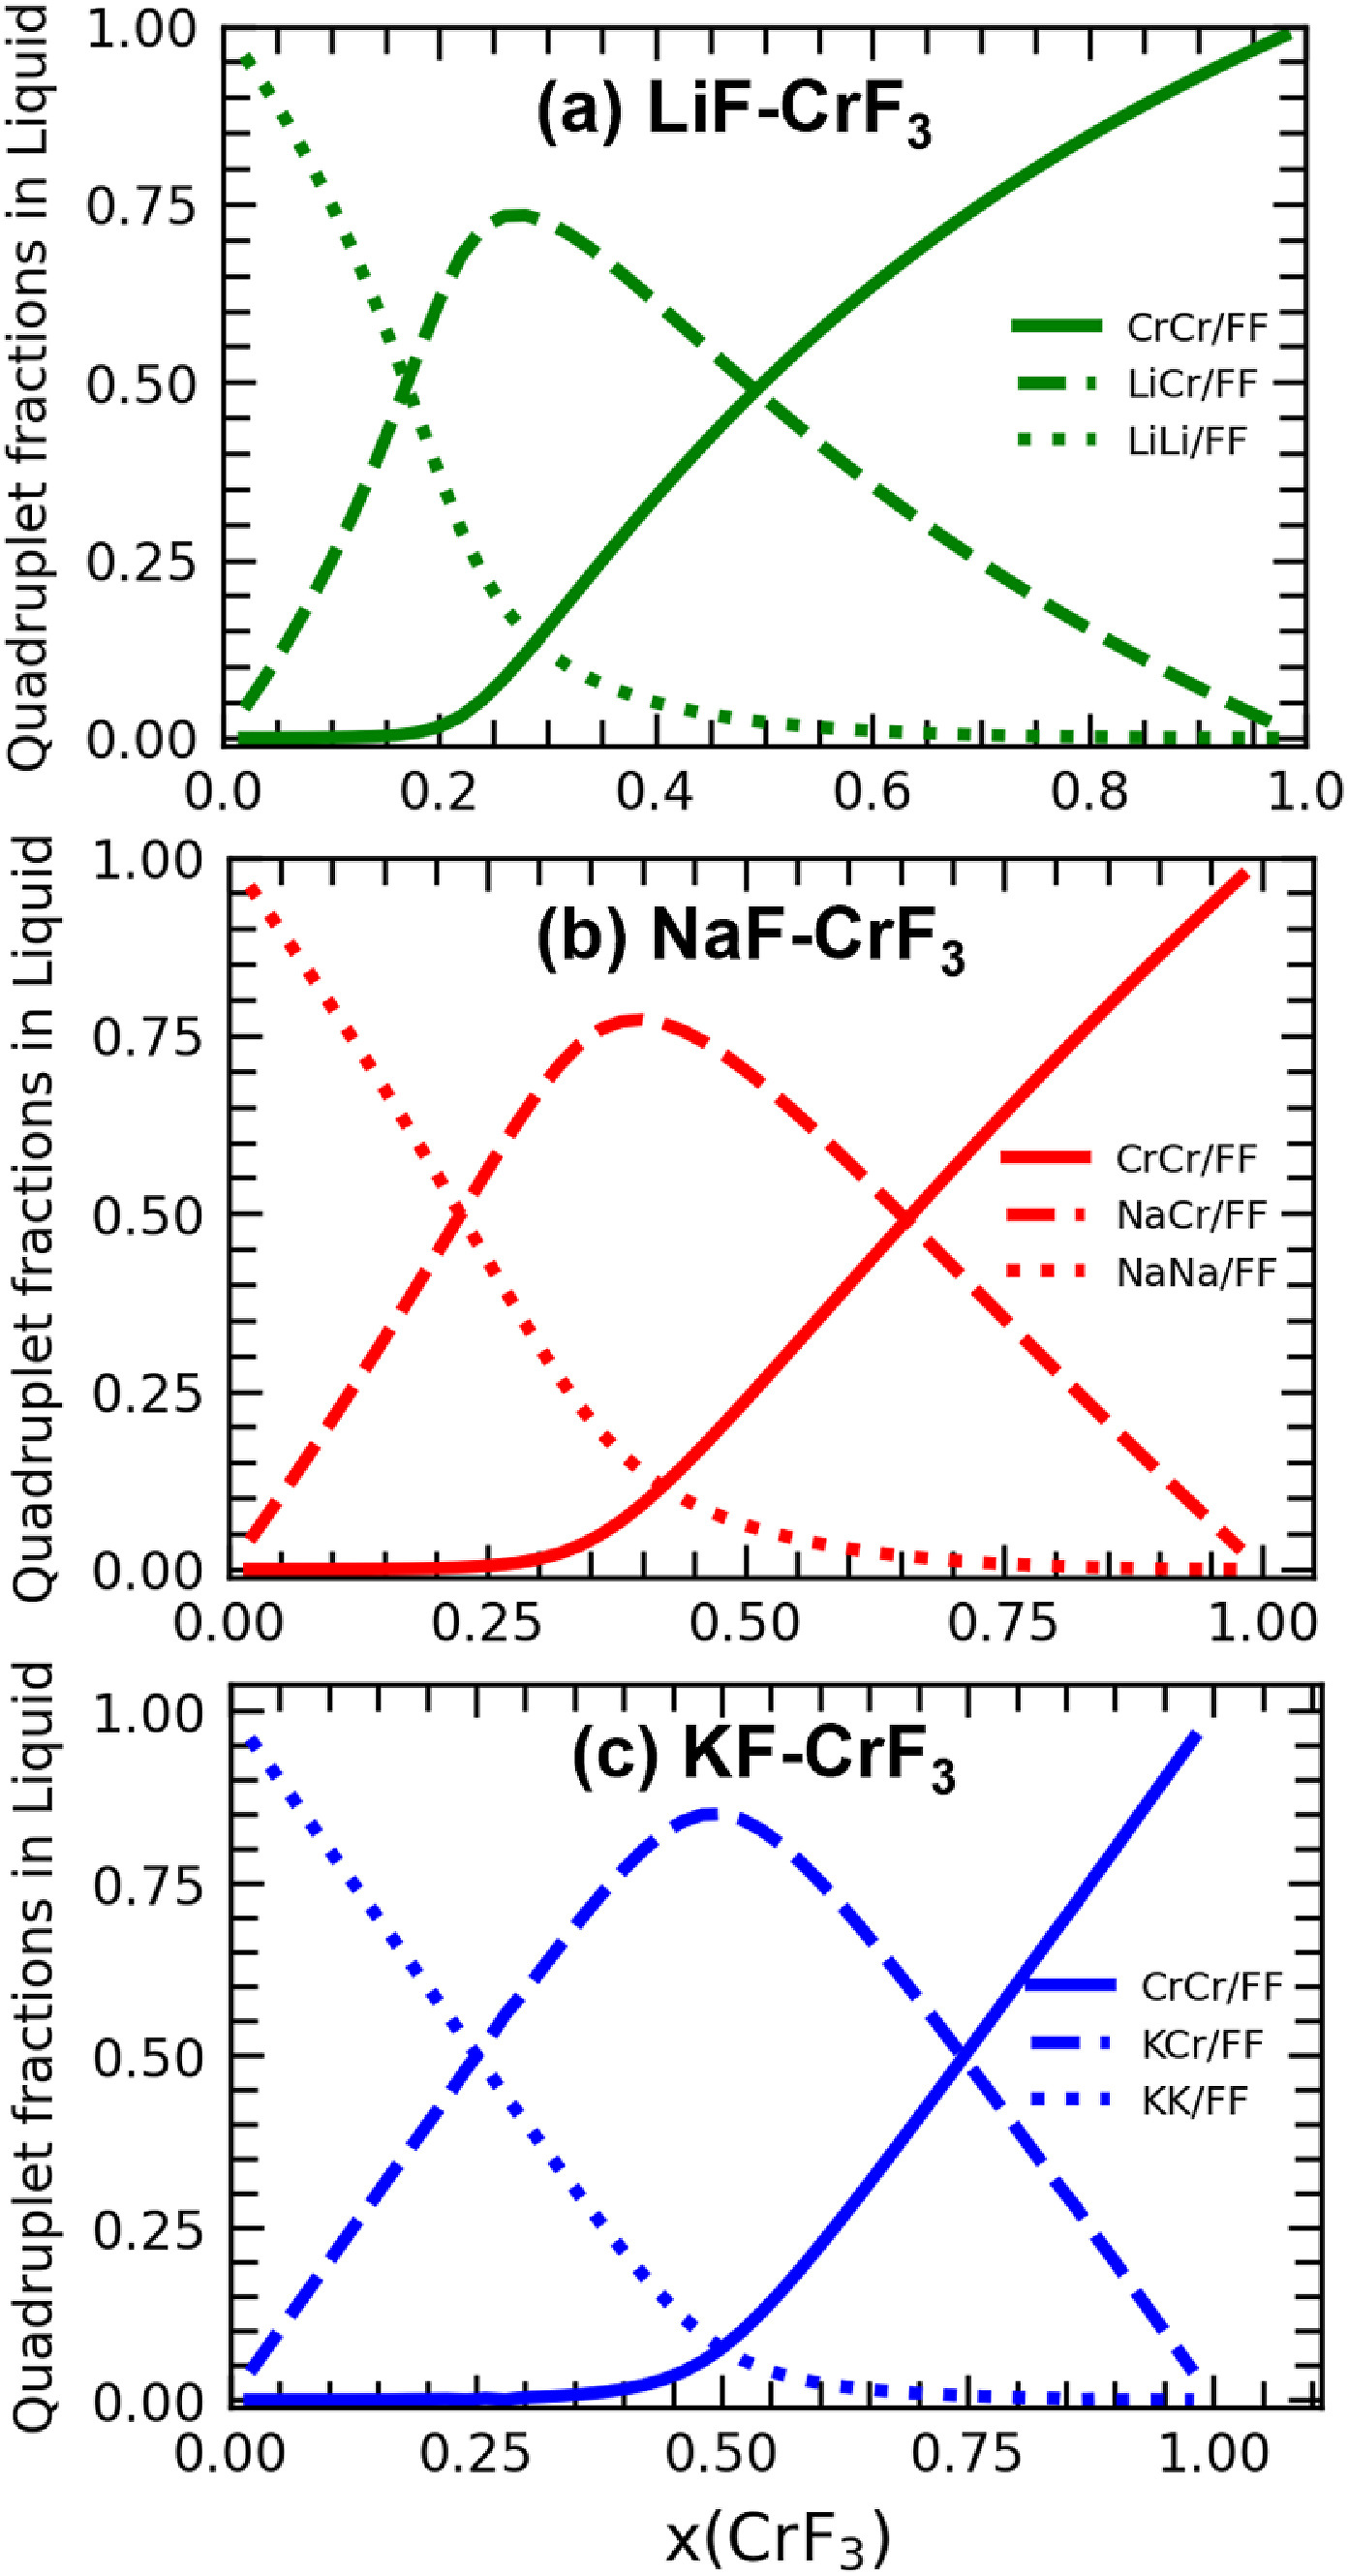
\includegraphics[width=0.45\linewidth]{moltensalts/Moltensalts-FLiNaKCr-QuadFrac.jpg}
    \caption{Precited quadruplet fractions in (a) LiF-CrF$_3$ (green lines), (b) NaF-CrF$_3$ (red lines), and (c) KF-CrF$_3$ (blue lines) liquid at 1700 K according to the present CALPHAD modeling. }
    \label{ms:fig:FLiNaKCr-QuadFrac}
\end{figure}

In Yin et al.’s modeling work \cite{yin2018thermodynamic}, the associate model was used to describe the liquid phase. This model was applied to describe the short-range ordering (SRO) by assuming ‘associates’, such as K$_3$CrF$_6$ and Na$_3$CrF$_6$ associates. This kind of assumption may cause issues when extrapolation into higher-order systems \cite{pelton2018phase}. In the present work, the MQMQA was employed to describe liquid and provide information on the first and the second nearest neighbors in complex liquid. As an example, Figure \ref{ms:fig:FLiNaKCr-QuadFrac} shows the predicted fraction of each quadruplet in the liquid phase. The composition where the peak fraction of the ACr/FF (A=Li, Na, and K) quadruplets appears, indicates the SRO. In the LiF-CrF$_3$ system, the peak fraction of LiCr:FF with strong SRO is around $x$(CrF$_3$) = 0.25, which is consistent with the lowest mixing enthalpy around the $x$(CrF$_3$) = 0.25 as shown in Figure \ref{ms:fig:FLiNaKCr-Hmix}. In addition, Figure \ref{ms:fig:FLiNaKCr-QuadFrac} presents the quadruplet fractions and the neighboring environments of ions in liquid, which are difficult to obtain from the associate model due to its focus on associate clusters.

\section{Bayesian model selection in thermodynamic modeling of LiCl-KCl-LaCl${_3}$} \label{moltensalts:sec:LaCl3}
In the CALPHAD community, several thermodynamic models, including the associate model, the two-sublattice ionic model, and the MQMQA, have been utilized to capture the complexity of molten salts. In the present work, the Bayes factor is used to guide the model selection process for thermodynamic modeling of the KCl-LaCl$_3$ system and provide statistical comparisons of various models. The results indicate that the MQMQA model is the most favorable based on available thermochemical data. The LiCl-KCl-LaCl$_3$ system has been further modeled with uncertainty quantification using MQMQA. Thermodynamic properties as a function of temperature for the compounds in KCl-LaCl$_3$ are predicted by the quasiharmonic approach in terms of first-principles phonon calculations. The calculated phase stability shows excellent agreement with experimental data, indicating that an appropriate thermodynamic model is important for accurately predicting the critical characteristics of complex molten salts.

The LiCl-KCl-LaCl$_3$ system contains the liquid phase, three binary compounds of LiCl, KCl, and LaCl$_3$, and two ternary compounds of K$_2$LaCl$_5$ and K$_3$La$_5$Cl$_{18}$ as summarized by Hao et al. \cite{hao2024thermodynamic}. K$_2$LaCl$_5$ was reported with a Pnma structure measured by Meyer et al. \cite{meyer1983k2mcl5}. Seifert et al. \cite{seifert1985thermodynamic} determined the structure of K$_3$La$_5$Cl$_{18}$ with a space group of $P6_3/m$ through X-ray diffraction. The values of formation enthalpy of K$_2$LaCl$_5$ and K$_3$La$_5$Cl$_{18}$ were measured by Seifert et al. \cite{seifert1985thermodynamic} using solution calorimetry. Reuter and Seifert \cite{reuter1994heat} reported the heat capacity values of K$_2$LaCl$_5$ and K$_3$La$_5$Cl$_{18}$ using differential scanning calorimetry (DSC). Gaune-Escard and Rycerz \cite{gaune1999heat} also measured the heat capacity of K$_3$La$_5$Cl$_{18}$ using DSC. Papatheodorou and Ostvold \cite{papatheodorou1974thermodynamic} reported mixing enthalpy in KCl-LaCl$_3$ through calorimetric experiments. Qiao et al. \cite{qiao1989measurement} utilized the differential thermal analysis (DTA) techniques to determine melting and phase transition temperatures. In the KCl-LaCl$_3$ system, Song and Zheng \cite{song1995investigation} measured liquidus by DTA. Seifert et al. \cite{seifert1985thermodynamic} measured phase boundaries in the LaCl$_3$-rich range by DTA.

In the ternary LiCl-KCl-LaCl$_3$ system, Bagri and Simpson \cite{bagri2016determination} and Samin et al. \cite{samin2016estimation} reported activity values for LaCl$_3$ in molten LiCl-KCl eutectic salt using electromotive force measurements and cyclic voltammetry, respectively. Regarding the phase diagram, Song and Zheng \cite{song1995investigation} reported the liquidus projection and six isopleths. Two research works, by Nakamura et al. \cite{nakamura1997thermal} and Venkata Krishnan et al. \cite{venkata2006pseudo}, constructed the pseudo-binary phase diagram from the LiCl-KCl eutectic to 25 mol\% of LaCl$_3$ in the LiCl-KCl eutectic through DSC.

\subsection{Modeling details} \label{moltensalts:ssec:LaCl3model}
Four frequently used models to describe complex molten salts are considered for the liquid phase in the KCl-LaCl$_3$, including the associate model \cite{sommer1982association}, the two-sublattice ionic model \cite{hillert1985two}, and the MQMQA \cite{pelton2001modified} (two sets of coordination numbers). 

The species KCl and LaCl$_3$ are assumed using the associate model \cite{sommer1982association} since no observation of other complex associates exists in the literature. The Gibbs energy of liquid can be expressed as: 
\begin{equation} \label{ms:eq:laassmG}
    \begin{aligned}
        G_m&=y_{\rm KCl}{{^o}G}_{\rm KCl}^{\rm Liquid}+y_{\rm {LaCl}_3}{{^o}G}_{\rm {LaCl}_3}^{Liquid}+RT\left(y_{KCl}\ln y_{\rm KCl}+y_{\rm {LaCl}_3}\ln y_{\rm {LaCl}_3}\right)\\&+y_{\rm KCl}y_{\rm {LaCl}_3}\sum_{v=0}{L_{\rm KCl,\rm {LaCl}_3}^v{(y_{\rm KCl}-y_{\rm {LaCl}_3})}^v}
    \end{aligned}
\end{equation}
where $y_i$ is the mole fraction of species $i$ (= KCl or LaCl$_3$), ${{^o}G}_i^{Liquid}$ the Gibbs energy of species $i$, $R$ the gas constant, and $L_{\rm KCl,{LaCl}_3}^v$ the $v^{th}$ interaction parameter, which can be expanded as in (\ref{method:eq:CEFLT}).

Using the two-sublattice ionic model \cite{hillert1985two}, the liquid phase in KCl-LaCl$_3$ can be described as: 
\begin{equation} \label{ms:eq:laionic}
    {({\rm K}^+,{\rm La}^{3+})}_P{({\rm Cl}^-)}_Q
\end{equation}
where the cations and anions are separated into two sublattices. The site ratios of $P$ and $Q$ follow the following relationships to maintain charge neutrality: 
\begin{equation} \label{ms:eq:laionicP}
    P=y_{{\rm Cl}^-}=1
\end{equation}
\begin{equation} \label{ms:eq:laionicQ}
    Q=y_{\rm K^+}+y_{{\rm La}^{3+}}
\end{equation}
where $y_i$ represents the mole fraction of ion $i$. The Gibbs energy function according to (\ref{method:eq:ionicGsrf}) and (\ref{method:eq:ionicScnf}) can be expressed as: 
\begin{equation} \label{ms:eq:laionicGm}
    G_m=y_{\rm K^+}{{^o}G}_{\rm KCl}^{Liquid}+y_{{\rm La}^{3+}}{{^o}G}_{{\rm LaCl}_3}^{Liquid}+RT\left(y_{\rm K^+}\ln y_{\rm K^+}+y_{{\rm La}^{3+}}lny_{{\rm La}^{3+}}\right)+{{^{xs}}G}_m 
\end{equation}
where ${{^{xs}}G}_m$ represents the excess Gibbs energy, which can be described based on the Redlich-Kister polynomial \cite{redlich1948algebraic} as described in (\ref{method:eq:ionicGxs}):
\begin{equation} \label{ms:eq:laionicGxs}
    {{^{xs}}G}_m=y_{\rm K^+}y_{{\rm La}^{3+}}\sum_{v=0}{L_{\rm K^+,{\rm La}^{3+}:{\rm Cl}^-}^v{(y_{K^+}-y_{{\rm La}^{3+}})}^v}
\end{equation}
where $L_{\rm K^+,{\rm La}^{3+}:{\rm Cl}^-}^v$ is the $v^{th}$ interaction parameter which can be described as in (\ref{method:eq:CEFLT}).

The MQMQA \cite{pelton2001modified} describes the KCl-LaCl$_3$ liquid phase by assuming interactions between the quadruplets of $\rm K_2{\rm Cl}_2$, ${\rm La}_2{\rm Cl}_2$, and ${\rm KLa}{\rm Cl}_2$. Coordination numbers $Z$ are defined to describe the second nearest neighbor coordination number of the species $i$ (= K, La, or Cl) in the quadruplets. $Z$ of anions can be calculated according to (\ref{method:eq:mqmqaZ}) to maintain charge neutrality. Coordination numbers used in the present work are summarized in Table \ref{ms:tab:lamqmZ}, where two sets of coordination numbers were applied to ${\rm KLa}{\rm Cl}_2$. The selection of MQMQA-M3 is based on Sun et al.’s modeling for KCl-NdCl$_3$ \cite{sun2004optimization}, while the MQMQA-M4 is based on the MSTDB-TC for KCl-LaCl$_3$ \cite{ard2022development}.

\begin{table}[H]
    \caption{Coordination numbers used in the present CALPHAD modeling with MQMQA for the liquid phase.}
    \centering
    \begin{tabular}{>{\raggedright\arraybackslash}m{1.5cm}>{\raggedright\arraybackslash}m{1.5cm}>{\raggedright\arraybackslash}m{3.5cm}>{\raggedright\arraybackslash}m{2.5cm}>{\raggedright\arraybackslash}m{2.5cm}>{\raggedright\arraybackslash}m{2.5cm}}
    \hline
    \textbf{A}&\textbf{B}&&$Z_{\rm AB:ClCl}^{\rm A}$&$Z_{\rm AB:ClCl}^{\rm B}$&$Z_{\rm AB:ClCl}^{\rm F}$ \\
    \hline
    K$^+$&K$^+$&&6.0&6.0&6.0\\
    La$^{3+}$&La$^{3+}$&&6.0&6.0&2.0\\
    K$^+$&La$^{3+}$&MQMQA-M3&2.0&6.0&2.0\\
    &&MQMQA-M4&3.5&6.0&2.55\\
    \hline
    \end{tabular}
    \label{ms:tab:lamqmZ}
\end{table}

The excess Gibbs energy is related to the formation Gibbs energy of the quadruplets as discussed in (\ref{method:eq:mqmqareac}). In the KCl-LaCl$_3$ system, this can be expressed as:
\begin{equation} \label{ms:eq:lamqmreac}
    \left(\rm K_2{\rm Cl}_2\right)_{quad}+\left({\rm La}_2{\rm Cl}_2\right)_{quad}=2\left(\rm KLa{\rm Cl}_2\right)_{quad}\;\;\;\;\Delta g_{\rm AB:Cl_2}^{ex}
\end{equation}
where $\Delta g_{\rm AB:Cl_2}^{ex}$ represents the Gibbs energy change when forming the quadruplets and can be described by: 
\begin{equation} \label{ms:eq:lamqmgex}
    \Delta g_{\rm AB:Cl_2}^{ex}=\Delta g_{\rm AB:Cl_2}^{o}+\sum_{(i+j)\geq1}{g_{\rm KLa:{\rm Cl}_2}^{ij}\chi_{\rm KLa:{\rm Cl}_2}^i\chi_{\rm LaK:{\rm Cl}_2}^j}
\end{equation}
where $g_{\rm KLa/{\rm Cl}_2}^{ij}$is a function of temperature and independent of composition. $\chi_{\rm KLa/{\rm Cl}_2}^i$ and $\chi_{\rm LaK/{\rm Cl}_2}^j$ are composition-dependent terms, defined as:
\begin{equation} \label{ms:eq:lamqmchi}
    \chi_{\rm KLa/{\rm Cl}_2}^i=\frac{X_{\rm K_2:Cl_2}}{X_{\rm K_2:Cl_2}+X_{\rm KLa:Cl_2}+X_{{\rm La}_2:{\rm Cl}_2}}
\end{equation}
where $X_{\rm KLa:Cl_2}$ is the fraction of $\left(\rm KLaCl_2\right)_{quad}$. 

All model parameters in the present work were optimized through the Bayesian approach using the MCMC method as implemented in ESPEI \cite{bocklund2019espei}. Each model parameter employed two Markov chains with a standard derivation of 0.1 when initializing its Gaussian distribution. During the modeling process, the chain values can be tracked and the MCMC processes were performed until the model parameters converged. The input data included primarily experimental phase equilibrium data for two or more co-existing phases, mixing enthalpy data, and activity data from the literature. For stochiometric compounds, their thermochemical data from DFT-based calculations were also used as input. 

The ternary compounds in the KCl-LaCl$_3$ system are considered stoichiometric compounds, including K$_2$LaCl$_5$ and K$_3$La$_5$Cl$_{18}$. Thermodynamic functions of the binary endmembers KCl and LaCl$_3$ are sourced from the JANAF tables \cite{chase1982janaf} and the SSUB database \cite{sgteurl}. The Gibbs energy for a given compound is expressed as in (\ref{ms:eq:Gstoi}). For these ternary compounds, their thermodynamic data including enthalpy, entropy, and heat capacity are obtained through DFT-based first-principles and phonon calculations. All DFT-based first-principles and phonon calculations in the present work were performed by the VASP \cite{kresse1996efficient}. The plane-wave basis cutoff energy was 262 eV for structural relaxations and 520 eV for the final static calculations of total energy. The convergent criterion of electronic self-consistency was set as $5\times10^{−6}$ eV/atom for relaxations and static calculations. Seifert et al. \cite{seifert1985thermodynamic} reported that K$_3$La$_5$Cl$_{18}$ possesses the symmetry of $P6_3/m$ with three Wyckoff sites of 2b, 2c, and 6h. However, the occupancy of the 2b site is less than 1, while the 2c site is occupied by both K and La atoms. Considering these, ATAT \cite{van2009multicomponent} was used to search for all possible configurations under these conditions, and 9 symmetry inequivalent configurations were found in terms of a 26-atom unit cell. The configuration with the lowest energy was predicted using DFT calculations. Phonon calculations were performed using the supercell method. Table \ref{ms:tab:ladftsetting} provides detailed settings for DFT-based first-principles and phonon calculations, including reciprocal k-points meshes and supercell sizes for phonon calculations, which ensures the convergence and accuracy of the DFT calculations.

\begin{table}[H]
    \caption{Details of the present DFT-based first-principles and phonon calculations for each compound, including space group, total atoms in the supercells, k-point meshes for structure relaxations, and the final static calculations (indicated by DFT), supercell sizes for phonon calculations, and k-point meshes for phonon calculations.}
    \centering
    \begin{tabular}{>{\raggedright\arraybackslash}m{2cm}>{\raggedright\arraybackslash}m{2cm}>{\raggedright\arraybackslash}m{3.5cm}>{\raggedright\arraybackslash}m{2.5cm}>{\raggedright\arraybackslash}m{2.5cm}>{\raggedright\arraybackslash}m{2.5cm}}
    \hline
    \textbf{Phase}&\textbf{Space Group}&\textbf{Atoms in crystallographic cell}&\textbf{k-points for DFT}&\textbf{Atoms in supercell for phonon}&\textbf{k-points for phonon}\\
    \hline
    KCl&$Fm\bar{3}m$&8&$8\times8\times8$&64&$3\times3\times3$\\
    LaCl$_3$&$P6_3/m$&8&$8\times8\times12$&64&$2\times2\times2$\\
    K$_2$LaCl$_5$&$Pnma$&32&$7\times7\times4$&32&$4\times4\times2$\\
    K$_3$La$_5$Cl$_{18}$&$P3$&26&$8\times8\times5$&26&$5\times5\times3$\\
    \hline
    \end{tabular}
    \label{ms:tab:ladftsetting}
\end{table}

\subsection{Thermodynamic properties in LiCl-KCl-LaCl$_3$ by first-principles calculations} \label{moltensalts:ssec:LaCl3DFTresult}
Thermodynamic properties of compounds in the KCl-LaCl$_3$ system were predicted using first-principles calculations. Table \ref{ms:tab:lacl3eosresults} summarizes the equilibrium properties of V$_0$, B$_0$, and B$^\prime$ at 0 K obtained by DFT-based calculations in comparison with experiments. The present work predicts the bulk modulus B$_0$ value to be 16.23 GPa for KCl, which is slightly lower than the experimental measurement of 19.7 GPa by Norwood et al. \cite{norwood1958elastic}. The equilibrium volume V$_0$ of LaCl$_3$ is predicted to be 27.37 \r{A}$^3$/atom in the present work, which is in good agreement with the measured 26.38 \r{A}$^3$/atom by Zachariasen \cite{Zachariasen1947}. It indicates that the present DFT calculations provide reliable predictions regarding the equilibrium properties of compounds in the KCl-LaCl$_3$ system. The present DFT calculations predicted the V$_0$ of K$_2$LaCl$_5$ to be 29.96 \r{A}$^3$/atom and B$_0$ to be 15.89 GPa. For K$_3$La$_5$Cl$_{18}$, the V$_0$ is reported to be 27.49 \r{A}$^3$/atom and B$_0$ to be 26.46 GPa.

\begin{table}[H]
    \caption{Predicted equilibrium properties of volume V$_0$, bulk modulus B$_0$, and the first derivative of bulk modulus with respect to pressure B$^\prime$ for compounds in the KCl-LaCl$_3$ system based on the present EOS fitting at 0 K. Experimental data are also listed for comparison.}
    \centering
    \begin{tabular}{>{\raggedright\arraybackslash}m{3cm}>{\raggedright\arraybackslash}m{3cm}>{\raggedright\arraybackslash}m{2.5cm}>{\raggedright\arraybackslash}m{2cm}>{\raggedright\arraybackslash}m{4cm}}
    \hline
    \textbf{Compounds}&\textbf{V$_0$}\ (\r{A}$^3$/atom)&\textbf{B$_0$}\ (GPa)&\textbf{B$^\prime$}&\textbf{Reference}\\
    \hline
    KCl&32.62&16.23&4.67&This work\\
    &&19.7&&Norwood et al. \cite{norwood1958elastic}\\
    LaCl$_3$&27.37&29.02&6.40&This work\\
	&26.38&&&Zachariasen \cite{Zachariasen1947}\\
    K$_2$LaCl$_5$&29.96&15.89&5.38&This work\\
    K$_3$La$_5$Cl$_{18}$&27.49&26.46&6.35&This work\\
    \hline
    \end{tabular}
    \label{ms:tab:lacl3eosresults}
\end{table}

Thermodynamic properties at finite temperatures are obtained through DFT-based QHA in terms of phonon. Figure \ref{ms:fig:lacl3pureQHA} compares the predicted values of heat capacity C$_p$, entropy $S$, and enthalpy $H-H_{300}$ of KCl and LaCl$_3$ to those from the SGTE database \cite{sgteurl}. For the KCl, the present QHA results align closely with the SGTE data \cite{sgteurl}, although the DFT values are slightly higher. The $S$ also shows a good agreement, with a minor difference of about 6\%. For the LaCl$_3$, the present QHA results slightly underpredict C$_p$ and $H-H_{300}$ compared to SGTE \cite{sgteurl}, particularly at higher temperatures. The differences in C$_p$ for LaCl$_3$ remain less than 3.2 J/mol-atom-K at high temperatures, while the entropy and enthalpy differences closely match the SGTE values \cite{sgteurl}. Figure \ref{ms:fig:lacl3CompoundsCp} shows the predicted heat capacities C$_p$ of K$_2$LaCl$_5$ and K$_3$La$_5$Cl$_{18}$ in comparison with experiments \cite{reuter1994heat, gaune1999heat}, demonstrating an excellent agreement. For example, at 500 K, QHA results show the K$_2$LaCl$_5$ C$_p$ of 26.99 J/mol-K, which is 0.8\% higher compared to 26.77 J/mol-K reported by Reuter et al. \cite{reuter1994heat} and 0.5\% higher than 26.86 J/mol-K by Gaune-Escard et al. \cite{gaune1999heat}. For K$_3$La$_5$Cl$_{18}$, the C$_p$ at 500 K is predicted to be 25.99 J/mol-K, slightly lower than 26.34 J/mol-K by Reuter et al. \cite{reuter1994heat}. These results of K$_2$LaCl$_5$ and K$_3$La$_5$Cl$_{18}$ obtained from the present DFT calculations are then used in the present CALPHAD modeling.

\begin{figure} [H]
    \centering
    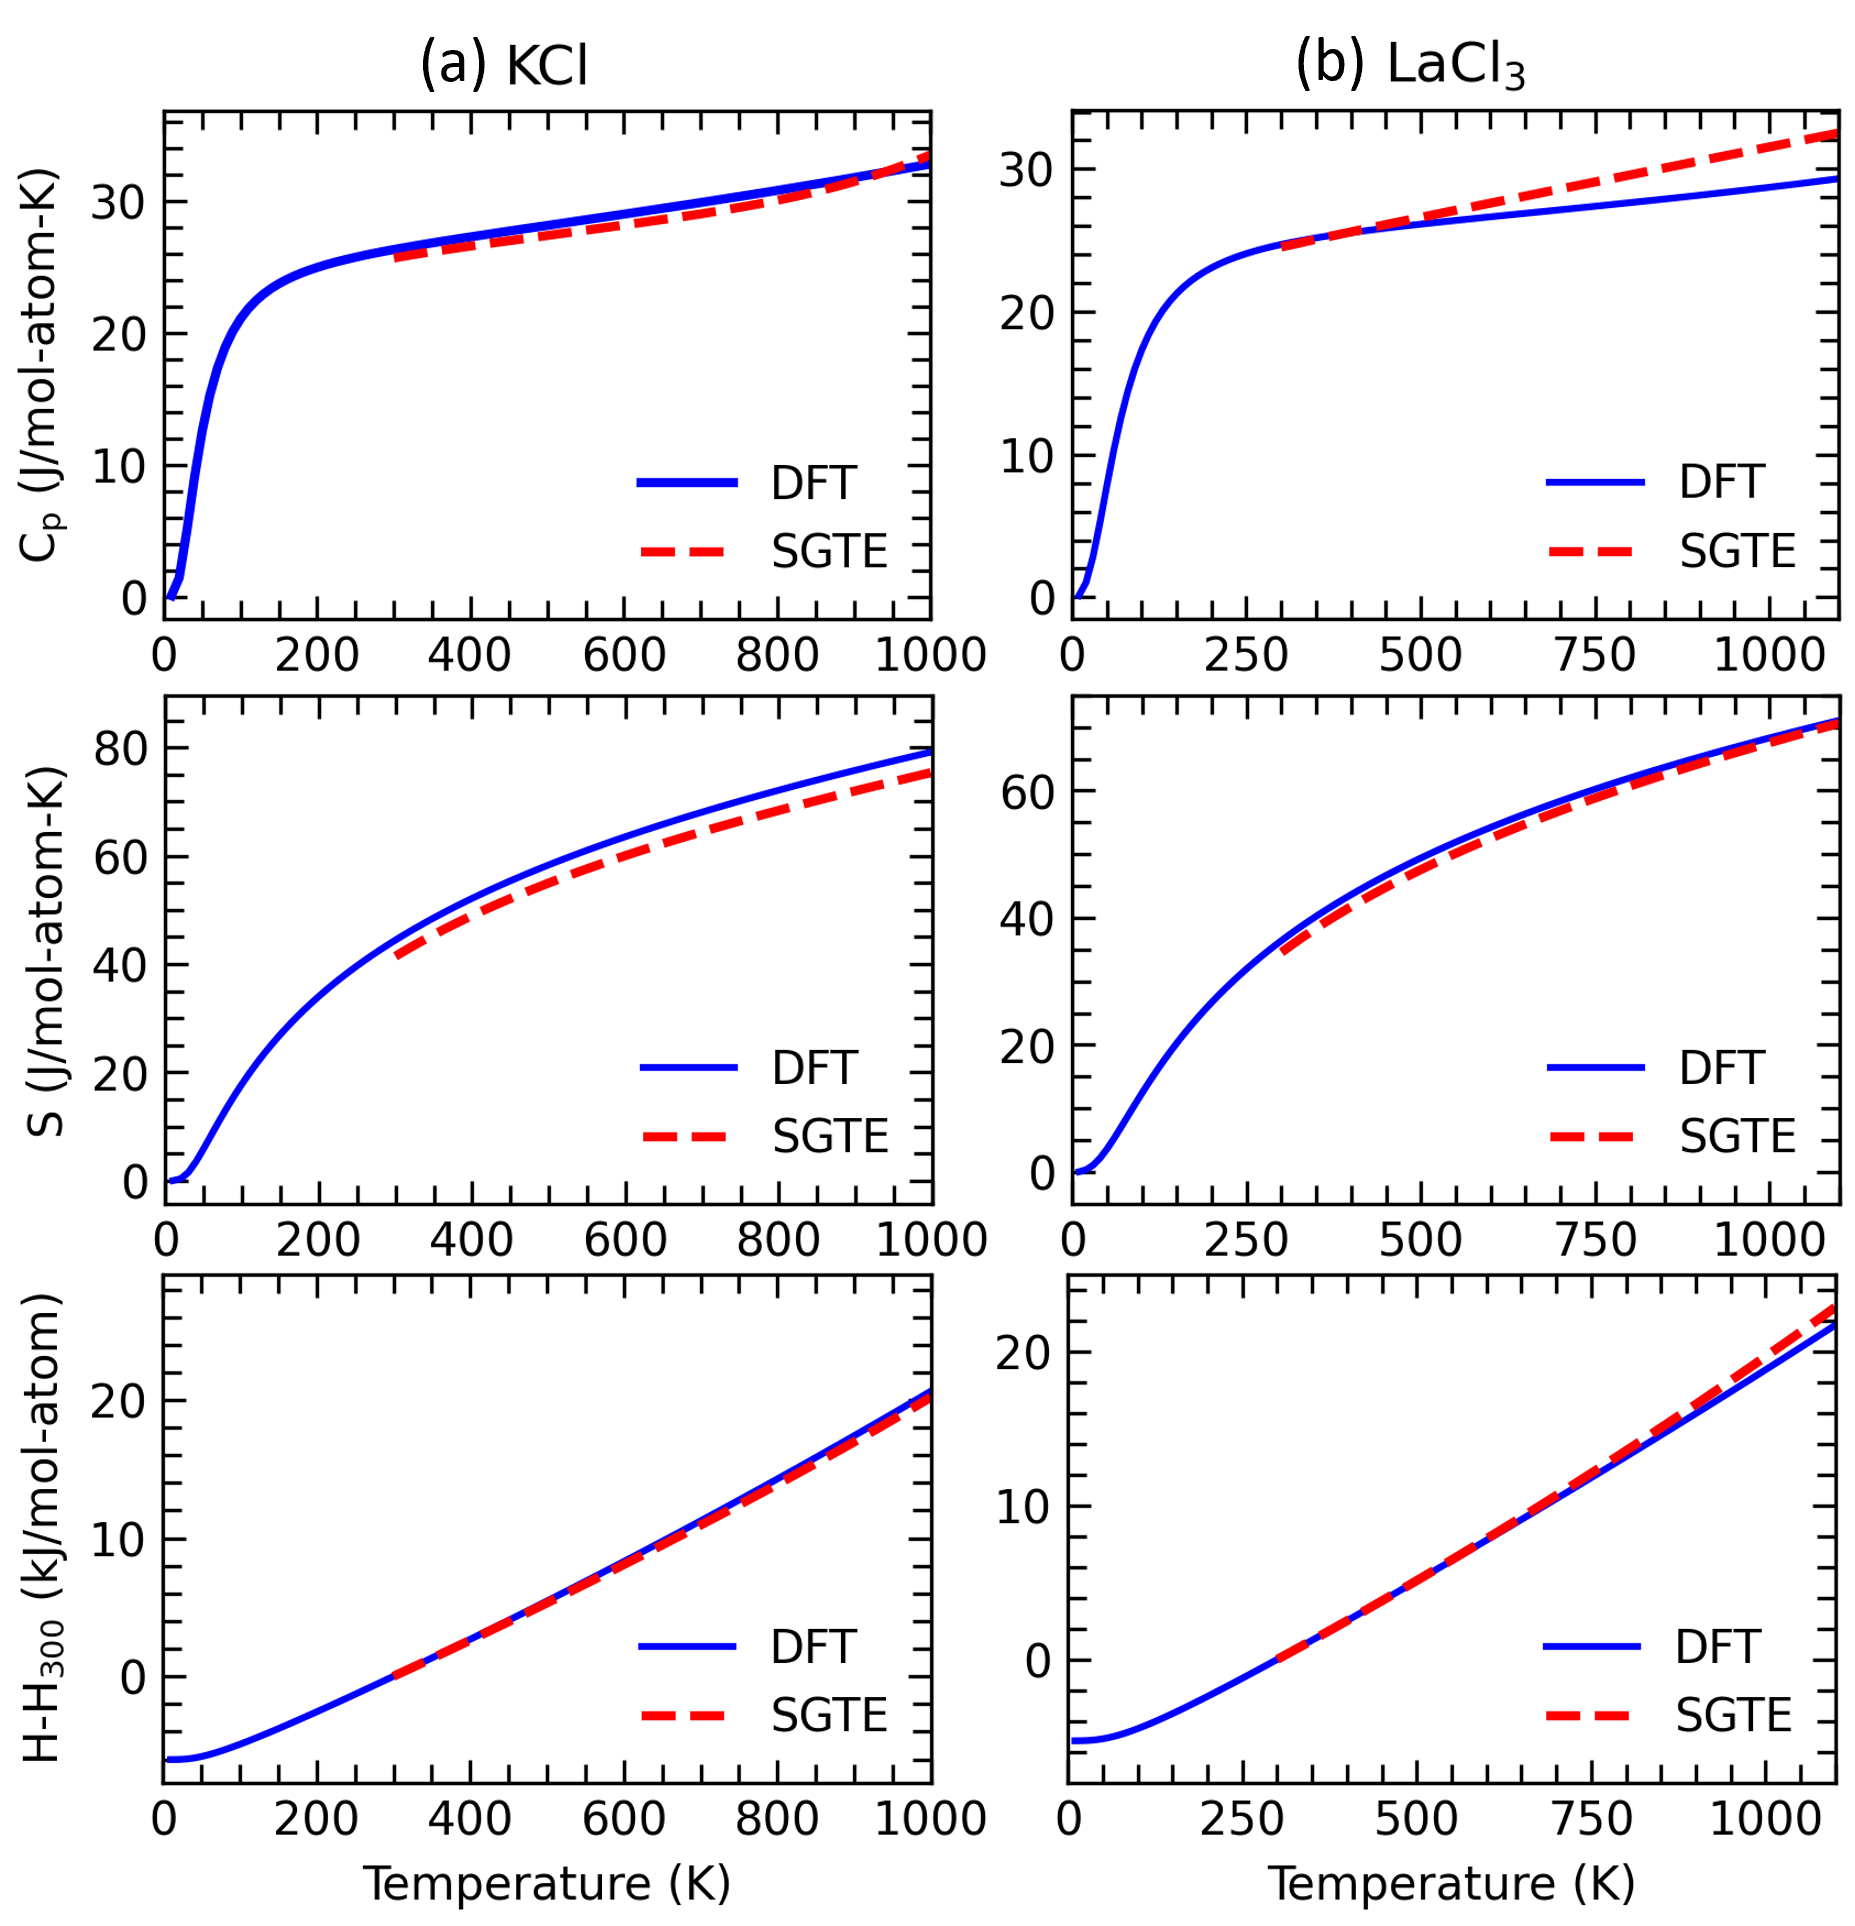
\includegraphics[width=0.9\linewidth]{moltensalts/Moltensalts-LaCl3-Cp-S-H.png}
    \caption{Comparison of the present values (blue lines) of heat capacity C$_p$, entropy $S$, and enthalpy with reference at 300 K ($H-H_{300}$) for (a) KCl and (b) LaCl$_3$ from the DFT-based phonon calculations (blue lines) with the SGTE data \cite{sgteurl} (red dash lines).}
    \label{ms:fig:lacl3pureQHA}
\end{figure}

\begin{figure} [H]
    \centering
    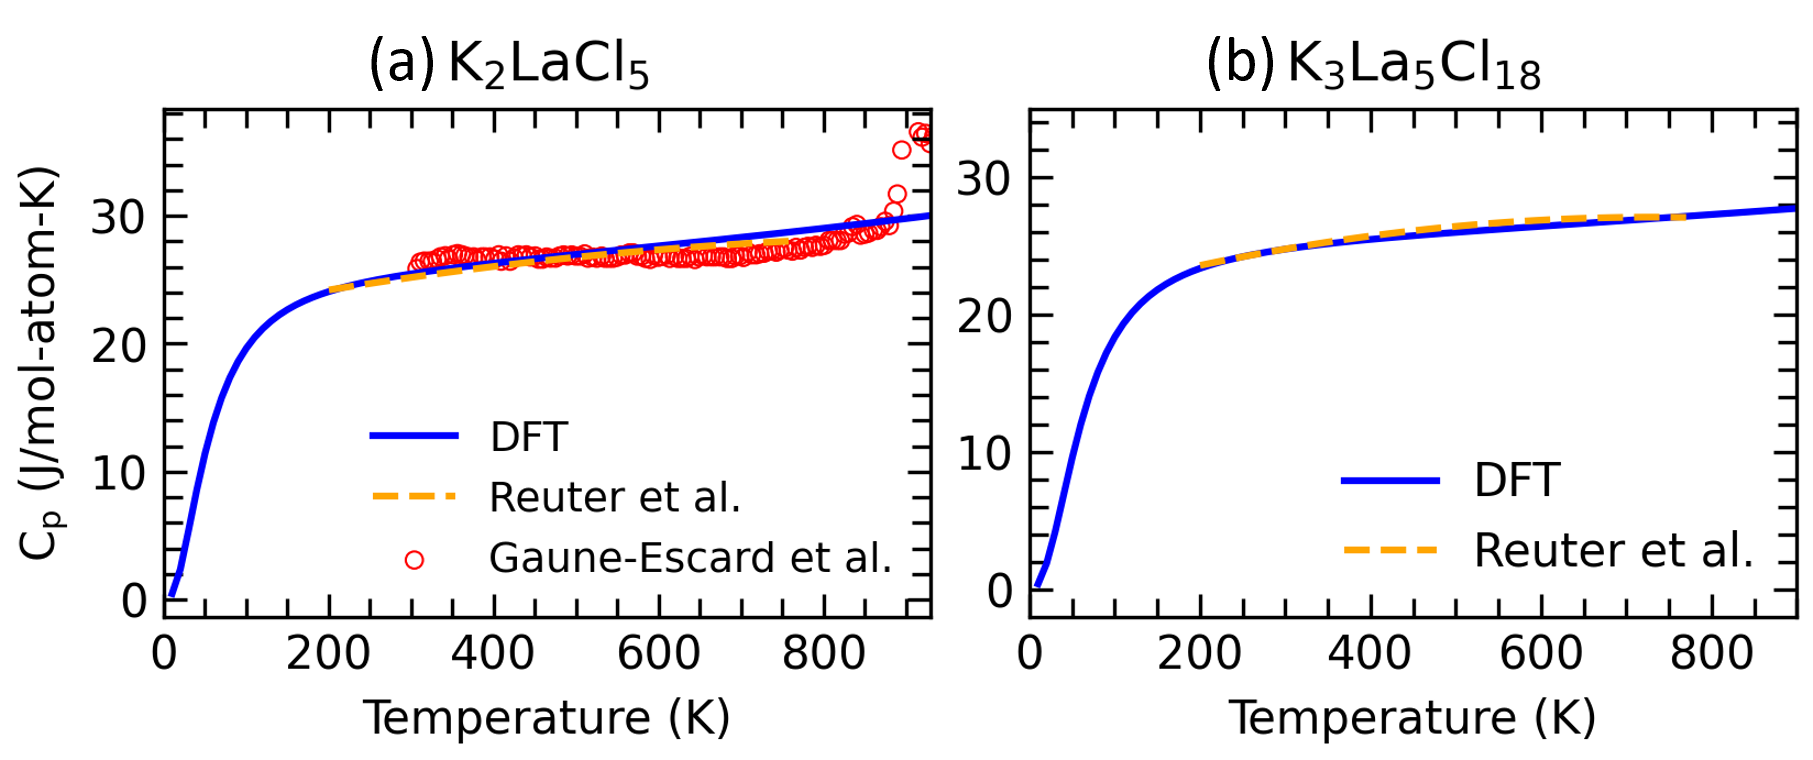
\includegraphics[width=0.9\linewidth]{moltensalts/Moltensalts-LaCl3-Compounds-Cp.png}
    \caption{Comparison of heat capacity C$_p$ values for (a) K$_2$LaCl$_5$ and (b) K$_3$La$_5$Cl$_{18}$ from the present DFT-based QHA (blue lines) with experiments by Reuter et al. \cite{reuter1994heat} (yellow dash lines) and Gaune-Escard et al. \cite{gaune1999heat} (red circles).}
    \label{ms:fig:lacl3CompoundsCp}
\end{figure}

\subsection{Model selection for the liquid phase in the KCl-LaCl$_3$ system} \label{moltensalts:ssec:LaCl3modelselection}
The KCl-LaC3 system is modeled using four models, the associate model (Associate-M1), the ionic model (Ionic-M2), and the MQMQA-M3 and the MQMQA-M4 with different coordination numbers as introduced in Section \ref{moltensalts:ssec:LaCl3model}. Experimental data are also listed for comparison. Each model has four adjustable parameters and was optimized by at least 1000 MCMC iterations. This process continued until the posterior probability values from each Markov chain stabilized, i.e., the model parameters converged. Figure \ref{ms:fig:lacl3PDfourm} compares the phase diagrams of these four models with experimental data \cite{seifert1985thermodynamic, song1995investigation}. It shows that for the liquidus of the KCl-rich region, MQMQA-M3 and MQMQA-M4 provide better agreements with experimental data than Associate-M1 and Ionic-M2. Table \ref{ms:tab:lacl3inv} lists the invariant reactions predicted by different models in comparison with experimental data \cite{seifert1985thermodynamic, song1995investigation}. All these four models show excellent agreement with the experimental data. Ionic-M2 and MQMQA-M4 slightly overpredict the invariant temperatures compared to those from Asscociate-M1 and MQMQA-M3. Specifically, Ionic-M2 and MQMQA-M4 predict a eutectic temperature of 854 K for the reaction of Liquid $\leftrightarrow$ KCl+K$_2$LaCl$_5$, which is 9 K higher than 845 K reported by Song et al. \cite{song1995investigation} and 1 K above 853 K by Seifert et al. \cite{seifert1985thermodynamic}. For the melting temperature of K$_2$LaCl$_5$, Ionic-M2 predicts 917 K, while MQMQA-M4 predicts 926 K, both are higher than the measured 913 K by Seifert et al. \cite{seifert1985thermodynamic} and 916 K by Song et al. \cite{song1995investigation}. Associate-M1 slightly underpredicts the peritectic temperature of the reaction Liquid+LaCl$_3$ $\leftrightarrow$ K$_3$La$_5$Cl$_{18}$ at 882 K, which is 3 K lower than the 885 K by Seifert et al. \cite{seifert1985thermodynamic} and the other models. The MAE for predicting these invariant temperatures using Associate-M1 is 2.5 K. MQMQA-M3 provides a good agreement with experimental data, with a slightly lower prediction of eutectic temperature for the reaction Liquid $\leftrightarrow $K$_2$LaCl$_5$+K$_3$La$_5$Cl$_{18}$ at 845 K, which is 6 K lower than 851 K reported by Seifert et al. \cite{seifert1985thermodynamic}. Regarding the invariant compositions $x$(LaCl$_3$), MQMQA-M3 and MQMQA-M4 offer better predictions with an MAE of 0.017 for both, compared to 0.025 for Associate-M1 and 0.022 for Ionic-M2. 

\begin{figure}[H]
    \centering
    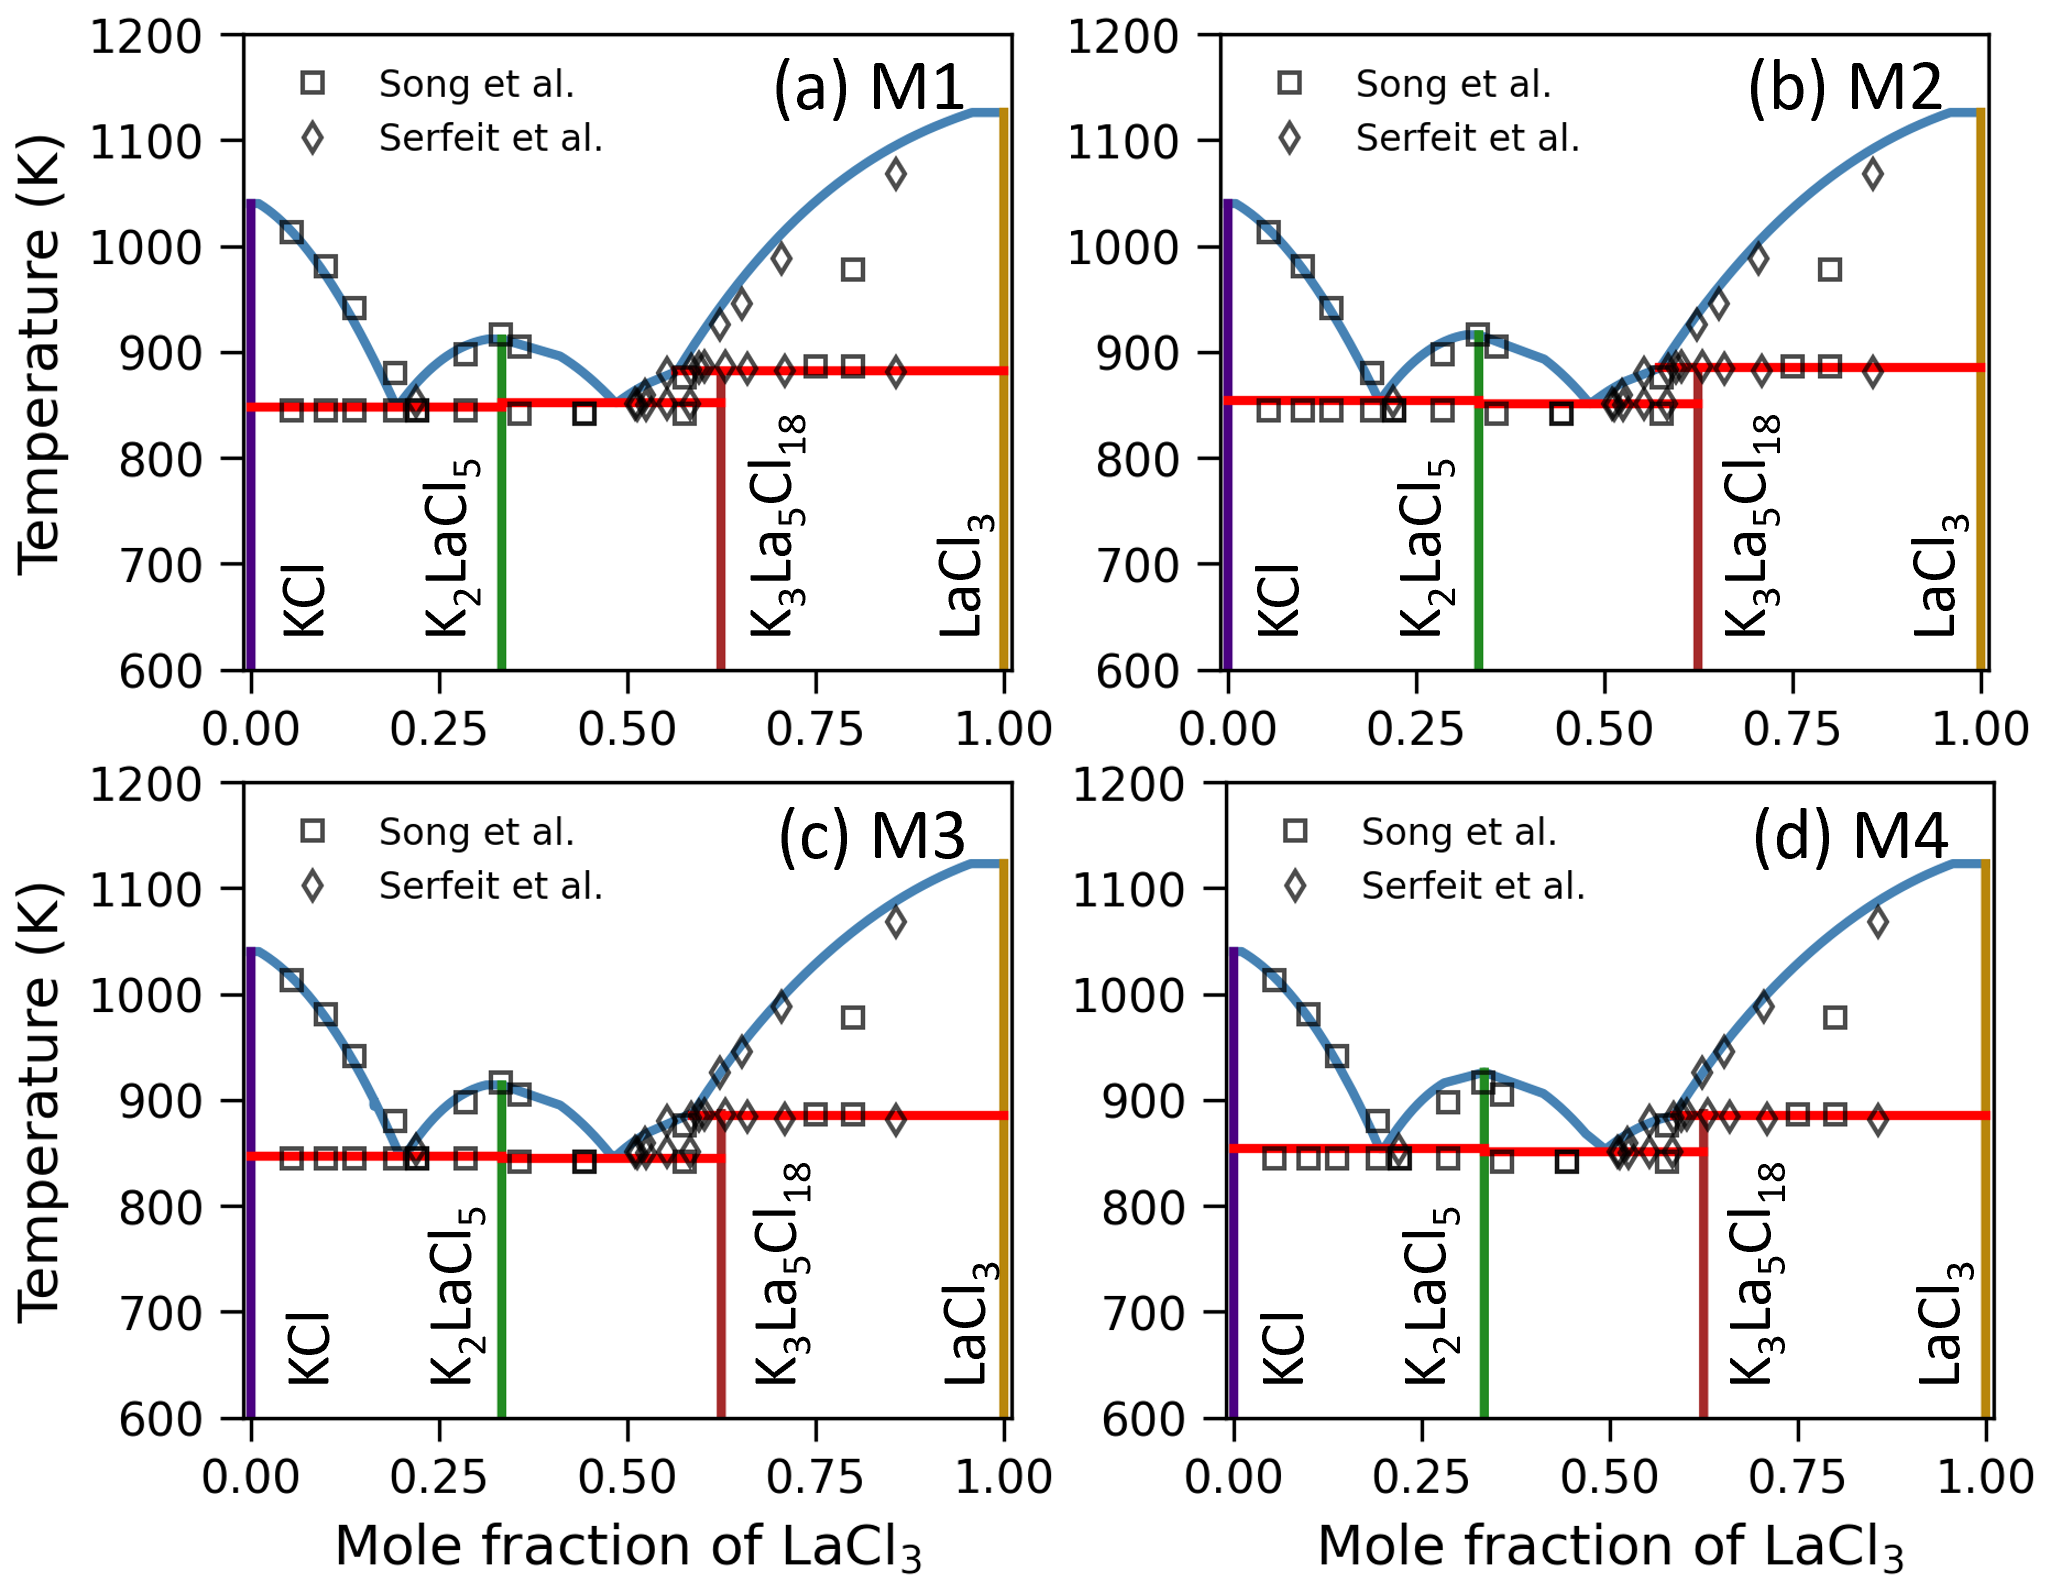
\includegraphics[width=0.9\linewidth]{moltensalts/Moltensalts-LaCl3-PhaseDiagram-Fourmodels-m.png}
    \caption{Predicted phase diagrams of the KCl-LaCl$_3$ system with the liquid phase modeled using (a) associate model (Associate-M1), (b) ionic model (Ionic-M2), (c) MQMQA (MQMQA-M3), and (d) MQMQA (MQMQA-M4) in comparison to experimental data \cite{seifert1985thermodynamic, song1995investigation}.}
    \label{ms:fig:lacl3PDfourm}
\end{figure}

\begin{table}[H]
    \caption{Predicted invariant equilibria in the KCl-LaCl$_3$ system by the four models, compared with experimental data.}
    \centering
    \begin{tabular}{>{\raggedright\arraybackslash}m{2cm}>{\raggedright\arraybackslash}m{5.5cm}>{\raggedright\arraybackslash}m{2cm}>{\raggedright\arraybackslash}m{2.5cm}>{\raggedright\arraybackslash}m{3.5cm}}
    \hline
    \textbf{Reaction}&&\textbf{$x$(LaCl$_3$)}&\textbf{Temperature} (K)&\textbf{Reference}\\
    \hline
    Eutectic&Liquid$\leftrightarrow$KCl+K$_2$LaCl$_5$&0.22&853&Seifert et al. \cite{seifert1985thermodynamic}\\
    &&0.22&845&Song et al. \cite{song1995investigation}\\
    &&0.197&848&Associate-M1\\
    &&0.202&854&Ionic-M2\\
    &&0.204&847&MQMQA-M3\\
    &&0.200&854&MQMQA-M4\\
    Melting&Liquid$\leftrightarrow$K$_2$LaCl$_5$&0.333&913&Seifert et al. \cite{seifert1985thermodynamic}\\
    &&0.333&916&Song et al. \cite{song1995investigation}\\
    &&0.333&913&Associate-M1\\
    &&0.333&917&Ionic-M2\\
    &&0.333&915&MQMQA-M3\\
    &&0.333&926&MQMQA-M4\\
    Eutectic&Liquid$\leftrightarrow$K$_2$LaCl$_5$+K$_3$La$_5$Cl$_{18}$&0.51&851&Seifert et al. \cite{seifert1985thermodynamic}\\
    &&0.485&852&Associate-M1\\
    &&0.481&851&Ionic-M2\\
    &&0.482&845&MQMQA-M3\\
    &&0.49&851&MQMQA-M4\\
    Peritectic&Liquid+LaCl$_3$$\leftrightarrow$K$_3$La$_5$Cl$_{18}$&0.595&885&Seifert et al. \cite{seifert1985thermodynamic}\\
    &&0.565&882&Associate-M1\\
    &&0.573&885&Ionic-M2\\
    &&0.586&885&MQMQA-M3\\
    &&0.586&885&MQMQA-M4\\
    \hline
    \end{tabular}
    \label{ms:tab:lacl3inv}
\end{table}

Figure \ref{ms:fig:lacl3HMRfourm} shows the values of mixing enthalpy of liquid at 1173 K calculated using these four models, compared with experimental data by Papatheodorou and Ostvold \cite{papatheodorou1974thermodynamic}. The comparison indicates that Associate-M1 and Ionic-M2 predict lower mixing enthalpy values than those by MQMQA-M3 and MQMQA-M4. For example, at $x$(LaCl$_3$) = 0.496, Associate-M1 predicts $-$15.469 kJ/mol and Ionic-M2 predicts $-$15.455 kJ/mol, slightly lower than the $-$15.097 kJ/mol predicted by MQMQA-M3 and $-$15.118 kJ/mol by MQMQA-M4. When compared to the mixing enthalpy value of $-$15.319 kJ/mol reported by Papatheodorou and Ostvold  \cite{papatheodorou1974thermodynamic}, Associate-M1 and Ionic-M2 show a closer alignment, with a difference of 0.9\%, compared to a 1.4\% difference for MQMQA-M3 and MQMQA-M4. Notably, Associate-M1 and Ionic-M2 align more closely with experimental data \cite{papatheodorou1974thermodynamic}, particularly in the composition region with $x$(LaCl$_3$) > 0.4. 

\begin{figure} [H]
    \centering
    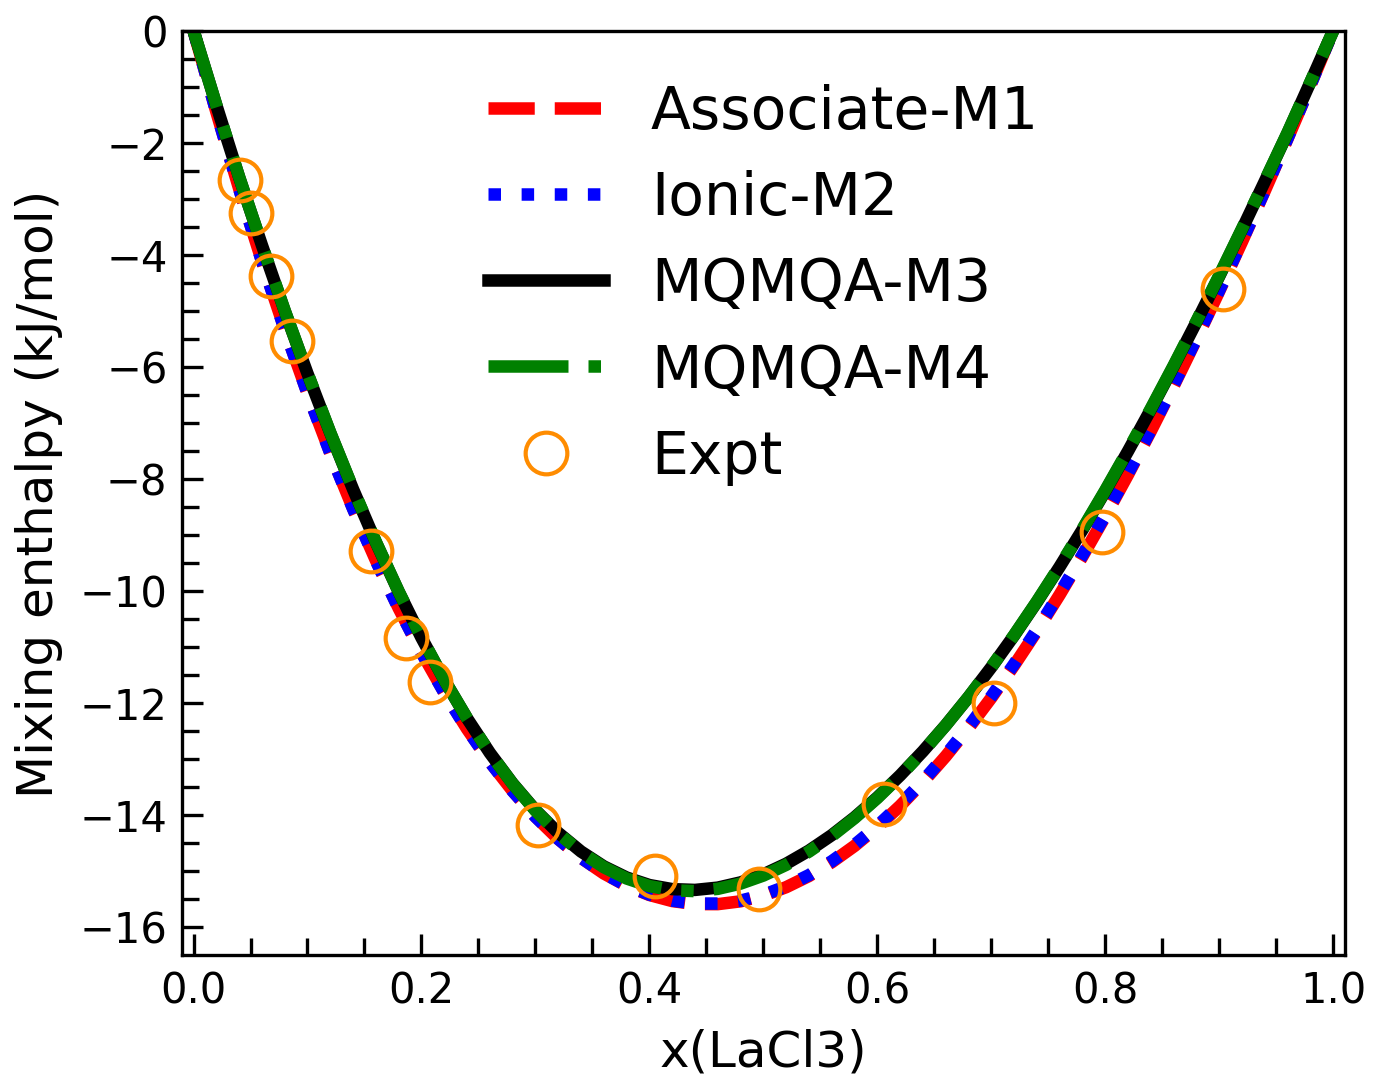
\includegraphics[width=0.5\linewidth]{moltensalts/Moltensalts-LaCl3-HMR-FourModels.png}
    \caption{Predicted values of mixing enthalpy of the KCl-LaCl$_3$ liquid at 1173K from four models in comparison with experimental data by Papatheodorou and Ostvold \cite{papatheodorou1974thermodynamic}. The red dash line represents Associate-M1, the blue dotted line represents Ionic-M2, the black solid line represents MQMQA-M3, and the green dash-dotted line represents MQMQA-M4.}
    \label{ms:fig:lacl3HMRfourm}
\end{figure}

According to phase diagrams (Figure \ref{ms:fig:lacl3PDfourm}) and mixing enthalpy predictions (Figure \ref{ms:fig:lacl3HMRfourm}), each model demonstrates a strength in predicting thermodynamic properties of the KCl-LaCl$_3$ system. Associate-M1 and Ionic-M2 perform well in predicting mixing enthalpy, showing a better match with experimental data as discussed above. However, these two models are less accurate in predicting phase boundaries compared to MQMQA-M3 and MQMQA-M4, especially in the LaCl$_3$-rich region. Choosing an appropriate model remains a challenge, as it requires balancing agreement with all available experimental data. A quantitative method is hence needed to determine the overall favorability for the models of study.

Bayesian parameter estimation through MCMC offers a powerful tool to statistically compare models, as demonstrated in Section \ref{method:ssec:Bayesian}. In the present work, the last 600 iterations from MCMC were used to compute the marginal likelihood $p\left(D\middle| M\right)$ for each model. Table \ref{ms:tab:lacl3bayesK} lists the estimated marginal likelihood value for each model, indicating that MQMQA-M3 has the highest marginal likelihood value of $\ln(p\left(D\middle| M_3\right))$ = $-370.628$. Consequently, the Bayes factors for the other models were calculated with respect to MQMQA-M3, using the marginal likelihood value of MQMQA-M3 as the numerator in (\ref{method:eq:BayesFactor}). The interpretation of the Bayes factor is also included in Table \ref{ms:tab:lacl3bayesK} according to the guideline by Kass and Raftery \cite{kass1995bayes}. That is, a ${log}_{10}({\rm Bayes factor})$ value between 0 and 1/2 suggests not worth more than a bare mention in comparing two models even if it points very slightly towards the model at the denominator, a range of 1/2 to 1 indicates substantial evidence in favor of the model at the denominator, 1 to 2 denotes strong evidence, and a value greater than 2 represents decisive evidence in favor of the model at the denominator. The present results indicate that the marginal likelihoods of Ionic-M2 $\ln(p\left(D\middle| M_2\right))$ = $-373.410$ and MQMQA-M4 $\ln(p\left(D\middle| M_4\right))$ = $-371.420$ are close to that of MQMQA-M3. In contrast, the marginal likelihood of Associate-M1 $\ln(p\left(D\middle| M_1\right))$ = $-439.135$ is significantly lower than that of MQMQA-M3, indicating that the Associate-M1 model is less favorable compared to the other three models. The Bayes factor ${log}_{10}K_{M3/M1}$ is 29.752, suggesting decisive evidence of favoring MQMQA-M3 over Associate-M1. This is due to the larger discrepancy in phase boundary predictions from Associate-M1 compared to the experimental phase diagram data shown in Figure \ref{ms:fig:lacl3PDfourm}(a). Regarding the Ionic-M2, the Bayes factor ${log}_{10}K_{M3/M2}$ = 1.208 indicates strong evidence of favoring MQMQA-M3 over Ionic-M2. Additionally, the Bayes factor comparing the two MQMQA models, ${log}_{10}K_{M3/M4}$, is 0.344, suggesting that MQMQA-M3 is slightly favored over MQMQA-M4, but not worth a bare mention when comparing these two models. It implies that the choice of these two sets of coordination numbers did not significantly affect the performance of MQMQA models in predicting thermodynamic properties in the KCl-LaCl$_3$ system. 

\begin{table}[H]
    \caption{Summary of the predicted marginal likelihood and Bayes factor for each model with respect to those of MQMQA-M3, and the suggested strength of evidence according to Kass and Raftery \cite{kass1995bayes}.}
    \centering
    \begin{tabular}{>{\raggedright\arraybackslash}m{3cm}>{\raggedright\arraybackslash}m{4.5cm}>{\raggedright\arraybackslash}m{4cm}>{\raggedright\arraybackslash}m{4.5cm}}
    \hline
    \textbf{Model name}&\textbf{Marginal likelihood ($\ln$ value)}&\textbf{Bayes factor $log_{10}K$}&\textbf{Strength of evidence}\\
    \hline
    Associate-M1&$-439.135$&29.752&Decisive\\
    Ionic-M2&$-373.410$&1.208&Strong\\
    MQMQA-M3&$-370.628$&-&-\\
    MQMQA-M4&$-371.420$&0.344&Not worth more than a bare mention\\
    \hline
    \end{tabular}
    \label{ms:tab:lacl3bayesK}
\end{table}

In summary, Bayesian parameter estimation through MCMC indicates that MQMQA-M3 is more favored, in terms of the input data of phase boundary and mixing enthalpy, over the other three models. This approach provides a robust technique for estimating the marginal likelihood values to assess the probability of data being generated by the model and calculating Bayes factors to statistically compare different models.

\subsection{Thermodynamic modeling of the LiCl-KCl-LaC$_3$ system} \label{moltensalts:ssec:LaCl3ternarymodeling}
The MQMQA-M3 is selected for the KCl-LaCl$_3$ system according to the Bayes factor. The ternary LiCl-KCl-LaCl$_3$ system is further improved by this model. The other two binary systems of LiCl-KCl and LiCl-LaCl$_3$ are taken from the MSTDB-TC \cite{ard2022development}. The available experimental data used for CALPHAD modeling include phase boundary data measured by Nakamura et al. \cite{nakamura1997thermal} and Venkata Krishnan et al. \cite{venkata2006pseudo}, activity data measured by Bagri and Simpson \cite{bagri2016determination} and Samin et al. \cite{samin2016estimation}, and mixing enthalpy data of LaCl$_3$ in LiCl-KCl eutectic. 

\begin{figure} [H]
    \centering
    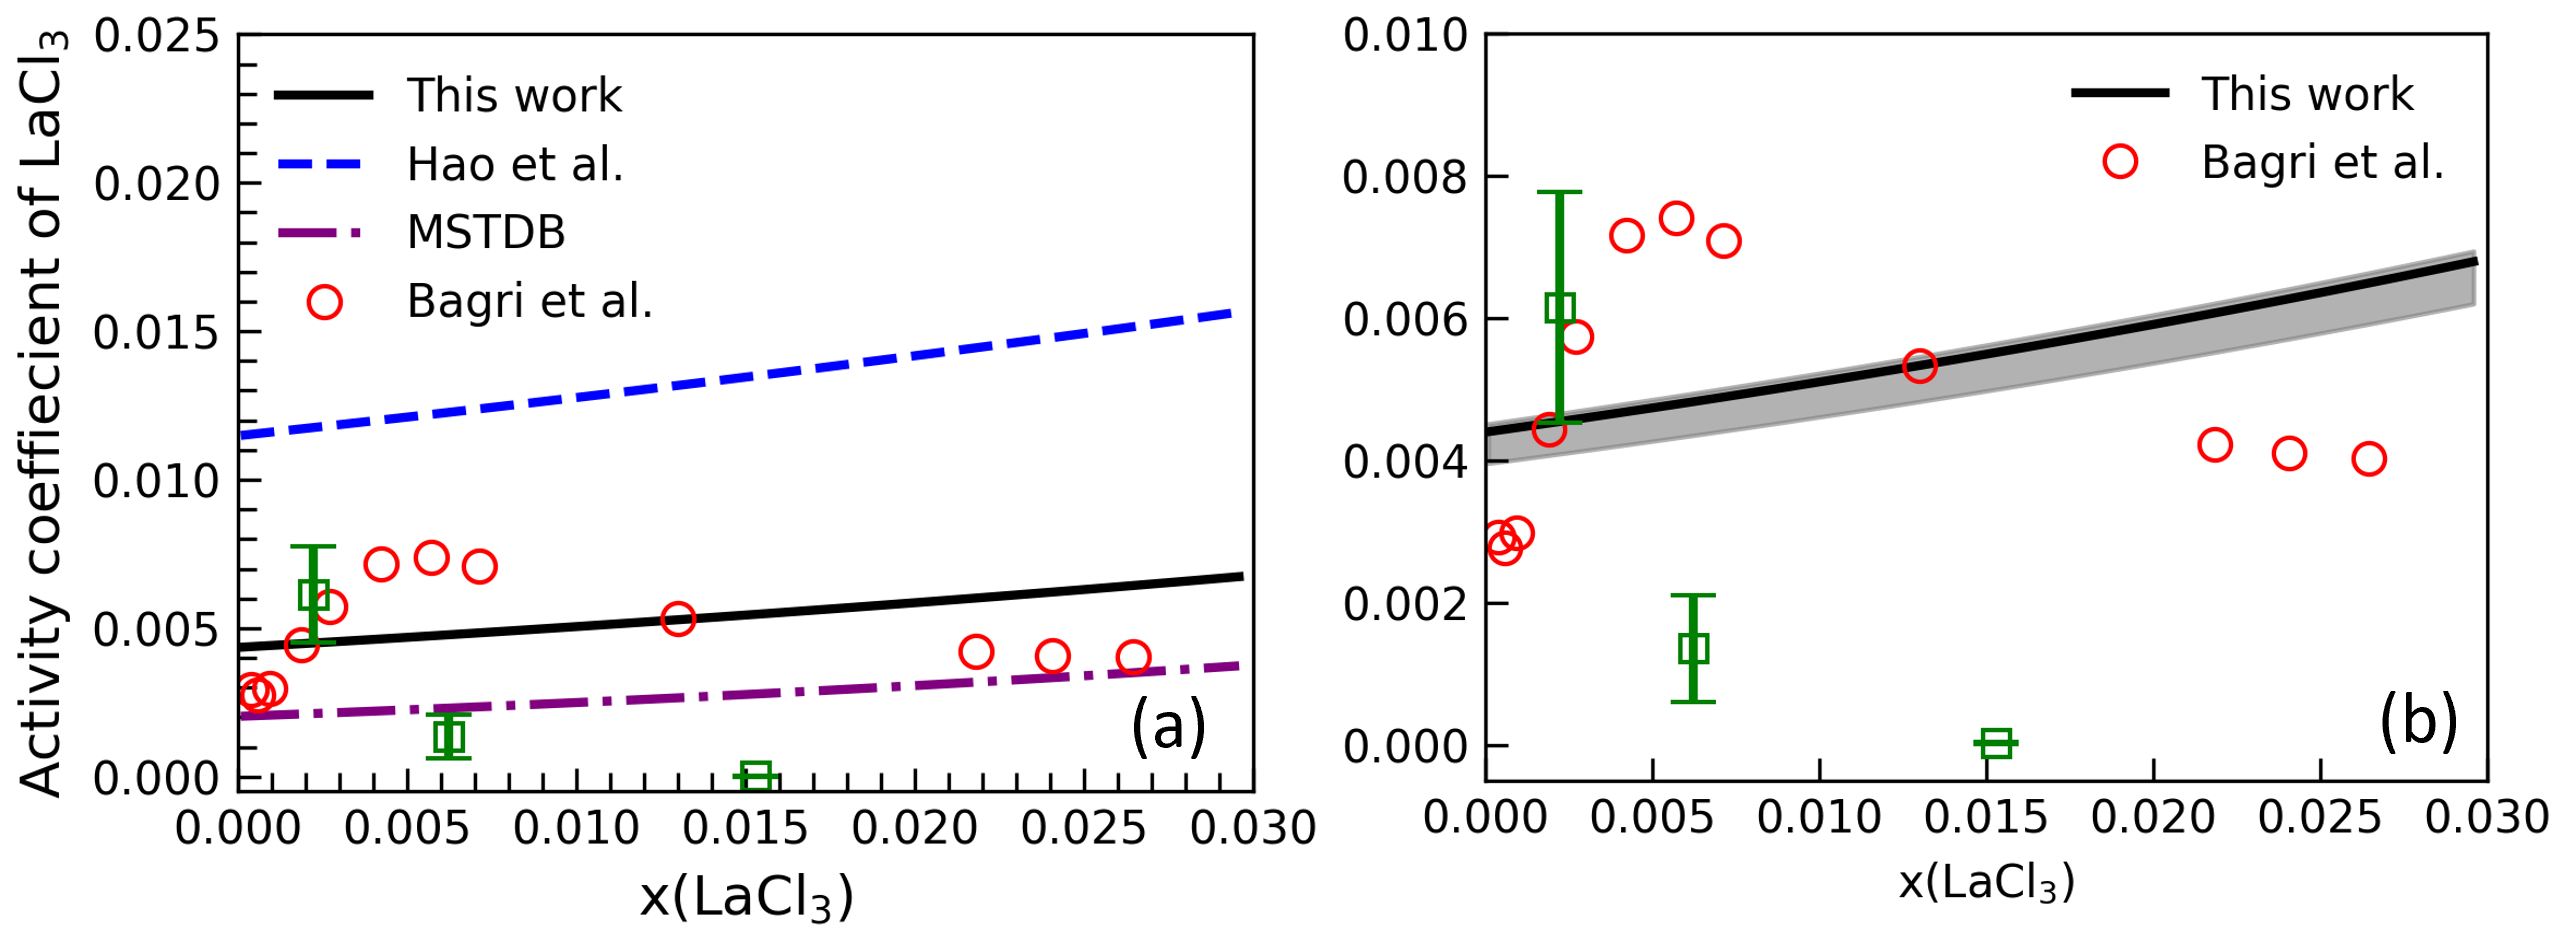
\includegraphics[width=1\linewidth]{moltensalts/Moltensalts-LaCl3-Gamma-Ternary-UQ.png}
    \caption{(a) Activity coefficients of LaCl$_3$ in KCl-LiCl eutectic at 773 K calculated from the present modeling in comparison with the modeling works from Hao et al. \cite{hao2024thermodynamic} (blue dash line) and MSTDB-TC \cite{ard2022development} (purple dash-dotted line), experimental measurements by Bagri et al. \cite{bagri2016determination} (red circles) and Samin et al. \cite{samin2016estimation} (green squares). (b) The uncertainty of the present modeling in predicting activity is shown in the grey region using a 95\% credible interval in predicting the activity values.}
    \label{ms:fig:lacl3ternaryGammaUQ}
\end{figure}

Thermodynamic properties predicted from the present CALPHAD modeling are compared with available experimental data. In addition, uncertainty quantification is performed to propagate parameter uncertainties into property predictions. Figure \ref{ms:fig:lacl3ternaryGammaUQ}(a) presents the values of the activity coefficient of LaCl$_3$ in the eutectic LiCl-KCl at 773 K, compared with the measurements by Bagri et al. \cite{bagri2016determination} and Samin et al. \cite{samin2016estimation}. The present modeling aligns more closely with the results by Bagri et al. \cite{bagri2016determination} since they provided a larger dataset over a broader composition range than those by Samin et al. \cite{samin2016estimation}. The model shows a good agreement in the low $x$(LaCl$_3$) region ($x$(LaCl$_3$) < 0.015) but slightly overestimates the activity coefficients when $x$(LaCl$_3$) increases to 0.02. The MAE of the present modeling, compared with values reported by Bagri et al. \cite{bagri2016determination}, is 0.0016. The present modeling represents a significant improvement over the previous work by Hao et al. \cite{hao2024thermodynamic}, which had an MAE of 0.0078 for predicting the activity coefficients. While MSTDB-TC \cite{ard2022development} shows a good agreement in the composition range of $x$(LaCl$_3$) from 0.022 to 0.027, it has a lower overall MAE of 0.0024 compared to the values reported by Bagri et al. \cite{bagri2016determination}. The present UQ values were performed using the last 10 MCMC iterations with 60 MCMC samples. The shadow region in Figure \ref{ms:fig:lacl3ternaryGammaUQ}(b) illustrates the uncertainties in predicting activity coefficients, with a 95\% credible interval (Bayesian credible intervals containing 95\% of the activity coefficients samples). This indicates that the present model has an uncertainty range of $-$10\% to +2\% in predicting the activity coefficient values.

\begin{figure} [H]
    \centering
    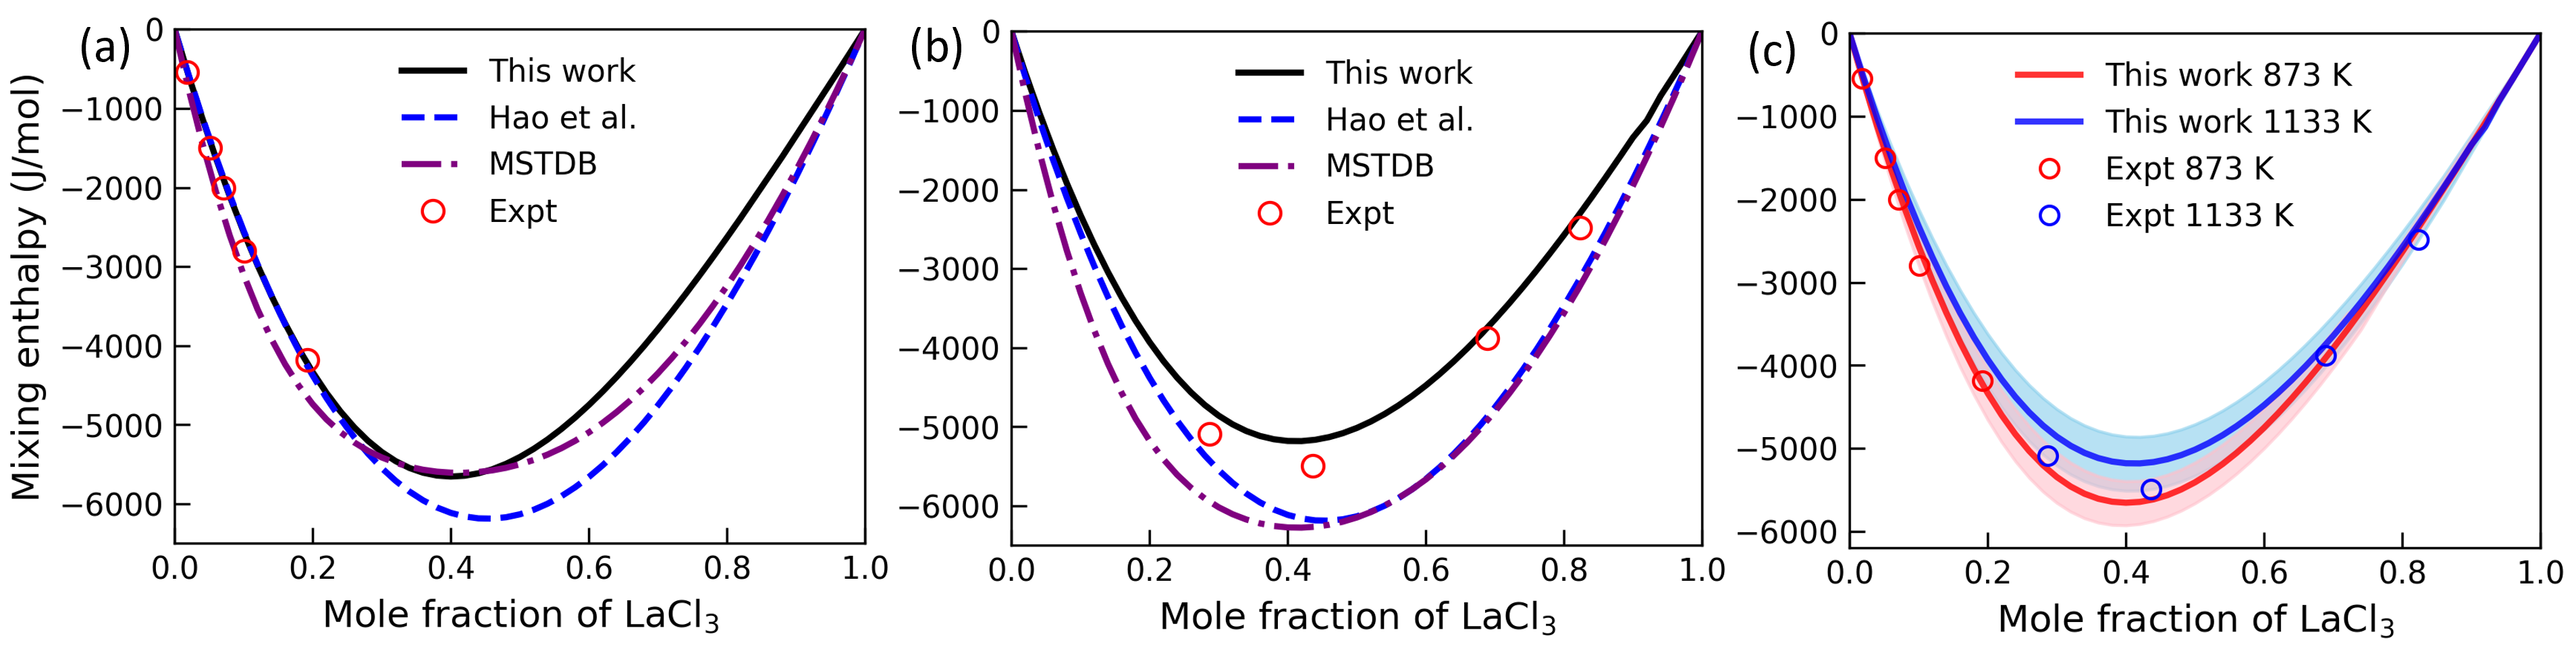
\includegraphics[width=1\linewidth]{moltensalts/Moltensalts-LaCl3-HMR-Ternary-UQ-models.png}
    \caption{Values of mixing enthalpy in LiCl-KCl-LaCl$_3$ at (a) 873 K and (b) 1133 K calculated from the present modeling compared with experimental measurements and the previous modeling works by Hao et al. \cite{hao2024thermodynamic} and MSTDB-TC \cite{ard2022development}. (c) The uncertainty of the present modeling in predicting mixing enthalpy is shown in the light red region (for 873 K) and the light blue region (for 1133 K) using a 95\% credible interval.}
    \label{ms:fig:lacl3ternaryHMRUQ}
\end{figure}


Figure \ref{ms:fig:lacl3ternaryHMRUQ} shows the mixing enthalpy calculations at 873 K and 1133 K from the present modeling, in comparison with experimental data and modeling results by Hao et al. \cite{hao2024thermodynamic} and MSTDB-TC \cite{ard2022development}. In Figure \ref{ms:fig:lacl3ternaryHMRUQ}(a), at 873 K, all these three modeling works closely match experimental measurements for $x$(LaCl$_3$) < 0.2. For example, at $x$(LaCl$_3$) = 0.1926, the present modeling predicts a mixing enthalpy of $-4231$ J/mol, which is 51 J/mol lower than the experimental value of $-4180$ J/mol. In comparison, Hao et al. \cite{hao2024thermodynamic} predicts $-4266$ J/mol and MSTDB-TC \cite{ard2022development} predicts $-4659$ J/mol, showing larger differences of 86 J/mol and 389 J/mol, respectively. The MAE of the present modeling in predicting mixing enthalpy at 873 K is 101 J/mol, compared to 120 J/mol for Hao et al. \cite{hao2024thermodynamic} and 312 J/mol for MSTDB-TC \cite{ard2022development}, highlighting the improved accuracy of the present modeling. Figure \ref{ms:fig:lacl3ternaryHMRUQ}(a) also shows different curve shapes in the LaCl$_3$-rich region predicted by three modeling works. The present modeling predicts a minimum energy similar to that by MSTDB-TC \cite{ard2022development} at around -5650 J/mol, whereas Hao et al. \cite{hao2024thermodynamic} predicts a value of $-6186$ J/mol, which is around 540 J/mol lower mixing enthalpy. Note that experiments investigations at 1133 K primarily focus on the LaCl$_3$-rich region.

Figure \ref{ms:fig:lacl3ternaryHMRUQ}(b) indicates that both Hao et al. \cite{hao2024thermodynamic} and MSTDB-TC \cite{ard2022development} predict lower values of mixing enthalpy compared to the present modeling and experiments. The present work improves the accuracy of mixing enthalpy predictions, reducing the MAE to 45.84 J/mol, compared to 159.75 J/mol by Hao et al. \cite{hao2024thermodynamic} and 183.30 J/mol by MSTDB-TC \cite{ard2022development}. Figure \ref{ms:fig:lacl3ternaryHMRUQ}(c) presents the uncertainty quantification of the present modeling in predicting mixing enthalpy, represented by the 95\% credible interval. At 873 K, the uncertainty range in predicting mixing enthalpy is around $-$5\% to +5\%. At 1133 K, the uncertainty range in predicting mixing enthalpy is around $-$6\% to +6\% with all existing experimental data falling within the lower boundary of the uncertainty region. This implies that the present modeling might underestimate the mixing enthalpy, particularly around $x$(LaCl$_3$) = 0.4. Further experiments or simulations in this composition range are recommended to enhance the accuracy of the present CALPHAD modeling. Figure \ref{ms:fig:lacl3quacf} shows the predicted fraction of each quadruplet in the liquid phase. The peak fractions of the LiLa/ClCl and LaK/ClCl quadruplets appear around $x$(LaCl$_3$) = 0.4, indicating the shorting range ordering (SRO) and it is consistent with the lowest mixing enthalpy around $x$(LaCl$_3$) = 0.4. 

\begin{figure} [H]
    \centering
    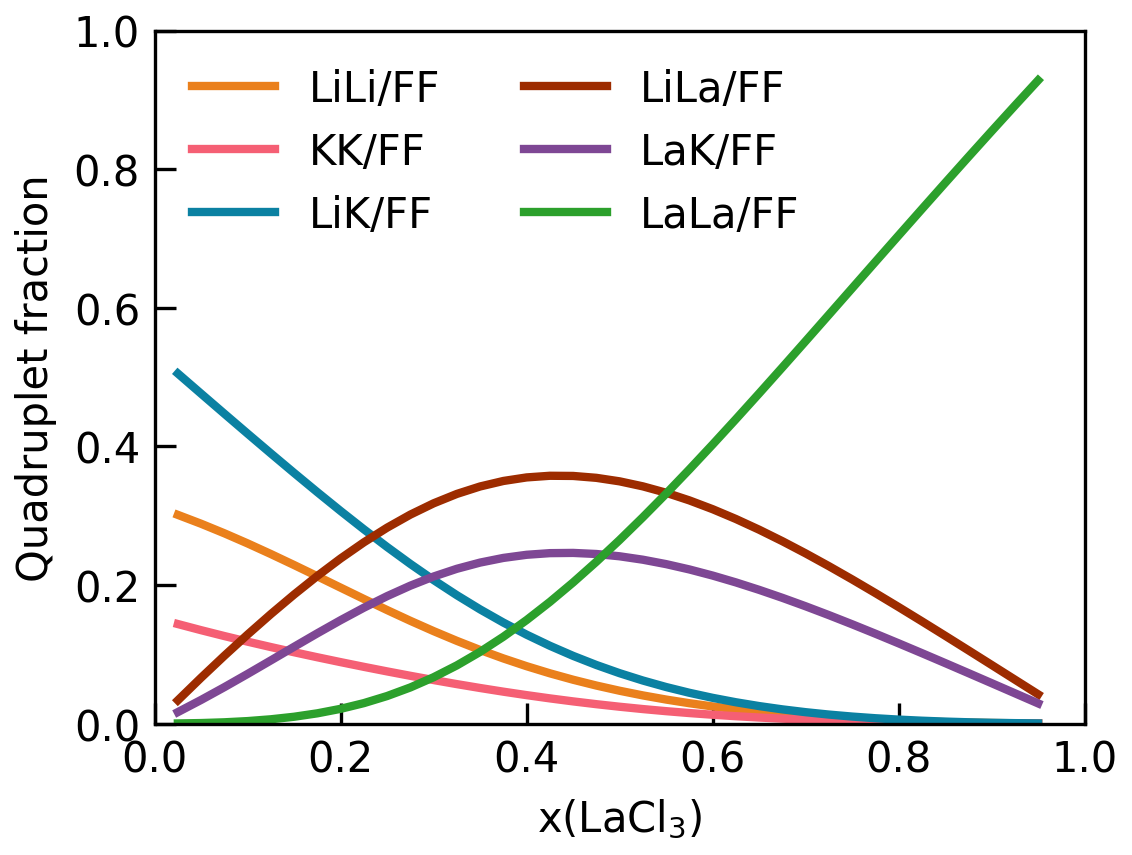
\includegraphics[width=0.6\linewidth]{moltensalts/Moltensalts-LaCl3-QuadFrac-LaCl3-LiCl-KCl.png}
    \caption{Precited quadruplet fractions in the LiCl-KCl-LaCl$_3$ liquid at 1133 K according to the present CALPHAD modeling using MQMQA.}
    \label{ms:fig:lacl3quacf}
\end{figure}

\begin{figure} [H]
    \centering
    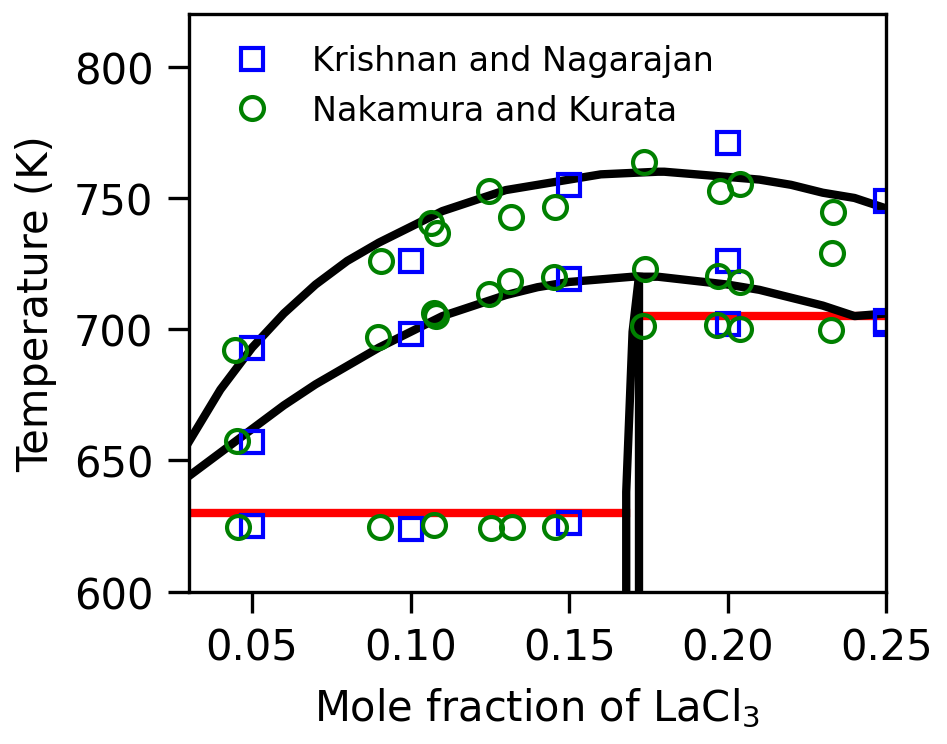
\includegraphics[width=0.6\linewidth]{moltensalts/Moltensalts-Isopleth-LaCl3-LiCl-KCl.png}
    \caption{Partial isopleth between the eutectic KCl-LiCl and LaCl$_3$ calculated from the present modeling work in comparison with experimental measurements by Venkata Krishnan et al. (blue squares) \cite{venkata2006pseudo} and Nakamura and Kurata (green circles) \cite{nakamura1997thermal}.}
    \label{ms:fig:lacl3ternaryisopleth}
\end{figure}

Figure \ref{ms:fig:lacl3ternaryisopleth} shows the partial isopleth between the eutectic KCl-LiCl and LaCl$_3$ calculated from the present CALPHAD modeling compared with experimental measurements \cite{nakamura1997thermal, venkata2006pseudo}, demonstrating a close match of liquidus and solidus lines. For the eutectic reaction Liquid$\leftrightarrow$KCl+LiCl\\+K$_2$LaCl$_5$, the present modeling predicts a eutectic temperature of 630 K, which is 5 K higher than the 625 K reported by Nakamura et al. \cite{nakamura1997thermal} and Venkata Krishnan et al. \cite{venkata2006pseudo}. Similarly, for the reaction Liquid$\leftrightarrow$LiCl+K$_2$LaCl$_5$+ K$_3$La$_5$Cl$_{18}$, the present modeling predicts the eutectic temperature at 705 K, which is 3 K higher than the reported 702 K by Nakamura et al. \cite{nakamura1997thermal} and Venkata Krishnan et al. \cite{venkata2006pseudo}. Overall, the present modeling of LiCl-KCl-LaCl$_3$ demonstrates a good agreement with experimental data \cite{bagri2016determination,samin2016estimation,nakamura1997thermal, venkata2006pseudo} regarding phase boundary properties. 

\section{Summary} \label{moltensalts:sec:Summary}
This chapter revisits the thermodynamic properties of compounds and liquids in the (LiF, NaF, KF, CrF$_2$)-CrF$_3$ systems by utilizing CALPHAD modeling with inputs from the DFT-based first-principles, phonon, and AIMD calculations. Thermodynamic properties, including enthalpy, entropy, and heat capacity of the binary (endmember) compounds LiF, NaF, KF, CrF$_3$, and CrF$_2$ as a function of temperature, have been predicted by DFT-based phonon calculations, agreeing with available experimental data in the literature and validating the reliability of the present methodology. They enabled the remodeling of the (LiF, NaF, KF, CrF$_2$)-CrF$_3$ systems with more accurate inputs. The MQMQA is employed to describe the liquid phase, providing valuable insights into the complex nature of molten salts such as the short-range ordering and neighboring of cations. Phase equilibria from the present CALPHAD modeling match better with experimental data in comparison with previous modeling work in the literature. The present thermodynamic data, including equilibrium volumes, bulk moduli, enthalpies, entropies, and heat capacities of compounds in the (LiF, NaF, KF, CrF$_2$)-CrF$_3$ system can be used to facilitate the development of advanced molten salt reactors.

In addition, this chapter demonstrates an application of Bayesian model selection to identify the optimal model for describing atomic environments in molten salts, focusing on the KCl-LaCl$_3$ system. Four candidate models are considered, which are the associate model, the two-sublattice ionic model, and two MQMQA models with different coordination numbers. By estimating the marginal likelihoods of each model from MCMC optimization and calculating Bayes factors to compare models, one of the MQMQA models is suggested as the most favorable one to describe the KCl-LaCl$_3$ system based on available input data. DFT-based calculations provide important thermodynamic properties for compounds in KCl-LaCl$_3$, including equilibrium volumes, bulk moduli, enthalpies, entropies, and heat capacities. Furthermore, the ternary LiCl-KCl-LaCl$_3$ system is modeled, demonstrating a better agreement with experimental data compared to the previous CALPHAD modeling works in the literature. The uncertainty quantification and propagation show that the present modeling provides reliable predictions of activity and mixing enthalpy when compared with experimental data. The present work indicates that the Bayesian model selection approach facilitates a more rational comparison among different liquid models, enhancing the accuracy of thermodynamic predictions in molten salts.

\chapter{Exploring and implementing thermodynamic models for complex liquid in open-source software PyCalphad} \label{chap:models}

\section{Introduction} \label{models:sec:intro}
For the modeling of complex liquids, Section \ref{method:ssec:liqmodels} discusses popular models within the CALPHAD framework, and Chapter \ref{chap:moltensalts} presents the applications in modeling of molten salts. Other models are also frequently applied in the chemical community to predict the nonideal mixing and phase behavior of small or large molecules. The UNIversal QUAsiChemical model (UNIQUAC) \cite{abrams1975statistical}, which considers the size and shape of ions in the solution, is currently being implemented into PyCalphad. The overall strategy for the implementation of UNIQUAC is based on three primary stages: (1) understanding and hard coding of the model, (2) representing the model through logic in code, and (3) using symbolic representation of variables used in PyCalphad as well as develop a parser for the database that use the UNIQUAC. The predicted thermochemical properties were compared with those from the OpenCalphad software \cite{li2020implementation} to verify the implementation work. Figure \ref{models:fig:implflow} shows the workflow for implementing custom models into PyCalphad and ESPEI. Moreover, a template generator is provided to expedite the process, creating templates for PyCalphad model classes and XML database schemas. These advancements provide the community with extensive opportunities to explore thermodynamic modeling with UQ in complex liquids such as molten salts, thereby making the existing databases continually updatable for the CALPHAD community and beyond. 

\begin{figure}[H]
    \centering
    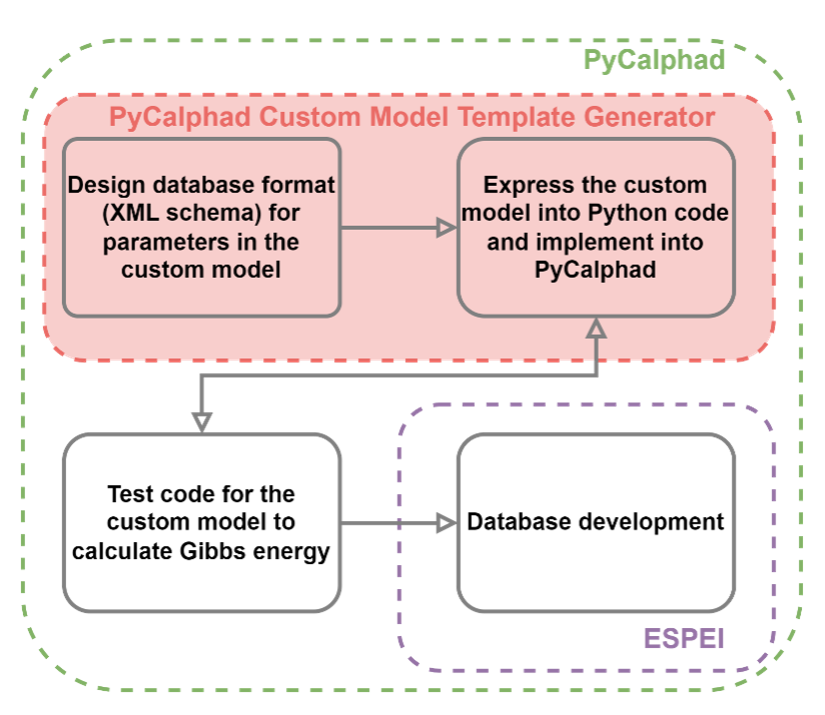
\includegraphics[width=0.75\linewidth]{models/Models-ImplementationFlow.png}
    \caption{Workflow for implementing custom models into PyCalphad and ESPEI.}
    \label{models:fig:implflow}
\end{figure}

\section{Implementation of UNIversal QUAsiChemical Model} \label{models:sec:UNIQUAC}
\subsection{UNIQUAC model} \label{models:ssec:UNIQUACfund}
The UNIQUAC model can be expressed using the CALPHAD nomenclature as follows:
\begin{equation} \label{models:eq:UQCGm}
    G_m=\sum_ix_i(^{o}G_i+RT\ln x_i) +\:^{cmb}G_m +\:^{res}G_m
\end{equation}
where $x_i$ is the mole fraction of constituent $i$, ${^o}G_i$ is the reference Gibbs energy of $i$, $\sum_ix_i^{o}G_i$ is considered as $^{srf}G_m$ term in (\ref{method:eq:Gm}). The second term $RT\sum_ix_i\ln x_i$ is configurational entropy contribution to Gibbs energy as $-T\:^{cnf}S_m$ term in (\ref{method:eq:Gm}). The excess Gibbs energy $^{xs}G_m$ are considered into two parts in the UNIQUAC, i.e., $^{cmb}G_m$ the combinatorial contribution of Gibbs energy and $^{res}G_m$ is the residual contribution of Gibbs energy.  

$^{cmb}G_m$ can be expressed as:
\begin{equation} \label{models:eq:UQCGcmb}
    ^{cmb}G_m=RT\sum_{i}{x_i\ln(\frac{\mathrm{\Phi}_i}{x_i}})+\frac{z}{2}\sum_{i}{x_iq_i\ln(\frac{\theta_i}{\mathrm{\Phi}_i}})
\end{equation}
\begin{equation} \label{models:eq:UQCphi}
    \mathrm{\Phi}_i=\frac{r_{i}x_i}{\sum_{j}{{r}_{j}x_j}}
\end{equation}
\begin{equation} \label{models:eq:UQCtheta}
    \theta_i= \frac{q_{i}x_i}{\sum_{j}{{q}_{j}x_j}}
\end{equation}
where $x_i$ is the mole fraction of constituent $i$, $r_i$ and $q_i$ are the component structural parameters, $r_i$ is the volume parameter, $q_i$ is the surface-area parameter, and $z$ is the average number of the nearest neighbors. $^{res}G_m$ can be expressed as:
\begin{equation} \label{models:eq:UQCres}
    {^{res}}G_m=-RT\sum_{i}{x_iq_i\ln(\rho_i})
\end{equation}
\begin{equation} \label{models:eq:rho}
    \rho_i=\sum_{j}{\theta_j\tau_{ji}}
\end{equation}
\begin{equation} \label{models:eq:UQCtau}
    \tau_{ji}=\exp \left(-\frac{u_{ij}-u_{ii}}{RT}\right)
\end{equation}
where $\Delta u_{ij}=u_{ij}-u_{ii}$ is the interaction parameter between $i$ and $j$, $u_{ii}$ represents the property of pure $i$. Thus, $\Delta u_{ij} \neq \Delta u_{ji}$ and $\tau_{ji} \neq \tau_{ij}$ Usually, $\Delta u_{ij}$ can be treated together as adjustable parameters during the modeling process.

%%%XML Database
To implement UNIQUAC into PyCalphad, a thermodynamic database containing the necessary parameters, such as $r_i$, $q_i$, and $\Delta u_{ij}$, is required. This database allows users to define these parameters, which PyCalphad can then read. To manage these newly defined parameters, an XML schema is employed as follows:
\begin{minted}[xleftmargin=1\parindent, linenos=true, fontsize=\small, breaklines=true]{xml}
<element name="Parameter">
    <attribute name="type">
        <choice>
            <value>UQCG</value><a:documentation>Gibbs energy of a specie</a:documentation>
            <value>UQCT</value><a:documentation>Tau function in residual contribution of excess Gibbs energy</a:documentation>
            <value>UQCQ</value><a:documentation>Surface-area parameter</a:documentation>
            <value>UQCR</value><a:documentation>Volume parameter</a:documentation>
            <value>UQCZ</value><a:documentation>Coordination number of a constituent</a:documentation>
        </choice>
    </attribute>
    <interleave>
        <optional>
            <text/>
        </optional>
        <zeroOrMore>
            <ref name="Interval"/>
        </zeroOrMore>
        <ref name="UNIQUACConstituentArray"/>
        <optional>
            <element name="Exponents">
                <list>
                    <data type="float"/>
                    <data type="float"/>
                </list>
            </element>
        </optional>
    </interleave>
</element>
\end{minted}
Here are the parts of the XML schema where parameters are defined. For example, by specifying \texttt{UQCQ}, the surface-area parameter $q_i$ can be defined. \texttt{UQCG} is the reference Gibbs energy ${^o}G_i$ in the (\ref{models:eq:UQCGm}), \texttt{UQCT} is the $\tau_{ji}$ function in residual contribution of excess Gibbs energy as shown in (\ref{models:eq:UQCtau}), \texttt{UQCR} is the volume parameter $r_i$, and \texttt{UQCZ} is the coordination number $z$.

The users now can adopt an XML thermodynamic database to input these parameters.
\begin{minted}[xleftmargin=1\parindent, linenos=true, fontsize=\small, breaklines=true]{xml}
<Parameter type='UQCQ'>1.72<ConstituentArray><Site refid="0"><Constituent refid="ACETONITRILE"/></Site></ConstituentArray></Parameter>
<Parameter type='UQCR'>1.87<ConstituentArray><Site refid="0"><Constituent refid="ACETONITRILE"/></Site></ConstituentArray></Parameter>
<Parameter type='UQCQ'>4.4<ConstituentArray><Site refid="0"><Constituent refid="N_HEPTANE"/></Site></ConstituentArray></Parameter>
<Parameter type='UQCR'>5.17<ConstituentArray><Site refid="0"><Constituent refid="N_HEPTANE"/></Site></ConstituentArray></Parameter>
<Parameter type="UQCZ">10<ConstituentArray><Site refid="0"><Constituent refid="ACETONITRILE"/></Site></ConstituentArray></Parameter>
<Parameter type="UQCZ">10<ConstituentArray><Site refid="0"><Constituent refid="N_HEPTANE"/></Site></ConstituentArray></Parameter>
<Parameter type="UQCT">exp(VV0001*T**(-1))<ConstituentArray><Site refid="0"><Constituent refid="ACETONITRILE"/><Constituent refid="N_HEPTANE"/></Site></ConstituentArray><Exponents>0.0 1.0</Exponents></Parameter>
<Parameter type="UQCT">exp(-545.71*T**(-1))<ConstituentArray><Site refid="0"><Constituent refid="ACETONITRILE"/><Constituent refid="N_HEPTANE"/></Site></ConstituentArray><Exponents>1.0 0.0</Exponents></Parameter>
\end{minted}

Here is an example of how to specify parameters for UNIQUAC in an XML thermodynamic database. First, define the type of parameter, such as \texttt{UQCQ}. Then, specify the value or function for that parameter. Following this, the name of the constituent can be defined using the \texttt{Constituent} tag.

\subsection{Calculations examples} \label{models:ssec:UNIQUACexamples}
With the implementation of the new UNIQUAC model in PyCalphad, users can automatically utilize all existing features in PyCalphad, including Gibbs energy minimization and phase diagram plotting. First, the calculation of Gibbs energy and its derivatives are carried out as a benchmark, comparing with calculation results from OpenCalphad \cite{li2020implementation}.

Figure \ref{models:fig:UQCGibbsE}, Figure \ref{models:fig:UQCS}, and Figure \ref{models:fig:UQCacr} depict the comparison between PyCalphad and OpenCalphad for calculating Gibbs energy, entropy, and activity, respectively. In PyCalphad, the \textit{calculate()} function was used to sample properties of a single phase, while the \textit{equilibrium()} function was utilized to perform global minimization of Gibbs energies and obtain phase equilibria. Both functions were thoroughly tested for UNIQUAC to ensure accurate calculations and minimization of Gibbs energy. The results demonstrate an excellent agreement between PyCalphad and OpenCalphad. The detailed value of Gibbs energy, entropy, and activity calculations are listed in Table \ref{models:tab:UQCGibbsE}, Table \ref{models:tab:UQCS}, and Table \ref{models:tab:UQCacr}, which shows that 0\% difference between calculations by PyCalphad and OpenCalphad. These calculations affirm the successful implementation of UNIQUAC in PyCalphad.

\begin{figure}[H]
    \centering
    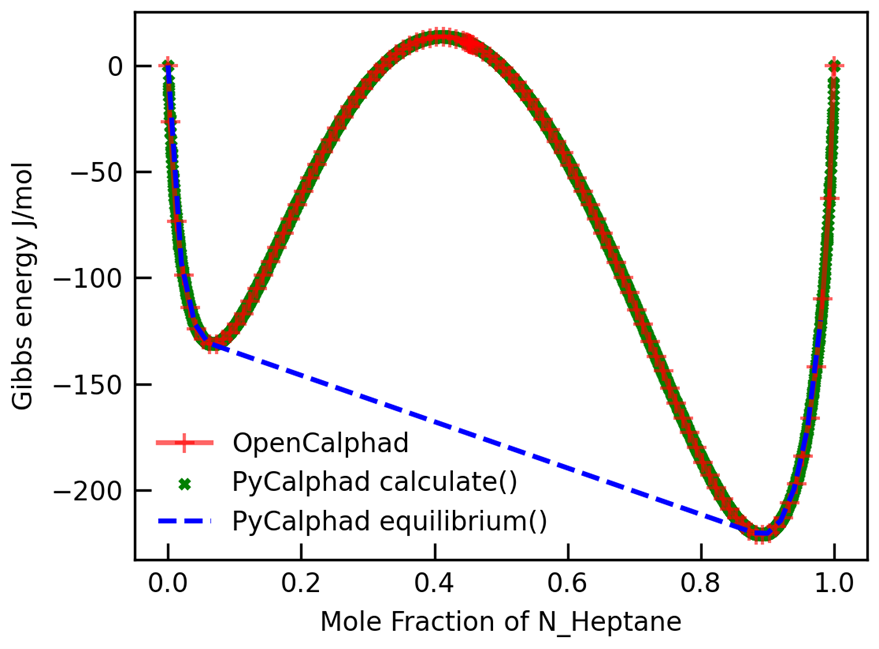
\includegraphics[width=0.5\linewidth]{models/Models-UQC-Gibbsenergy.png}
    \caption{Comparison of PyCalphad with OpenCalphad calculating Gibbs energy to verify the implementation of UNIQUAC. The red line represents results from OpenCalphad, the green $\times$ symbols represent results from the PyCalphad \textit{calculate()} function, and the blue line represents results from the PyCalphad \textit{equilibrium()} function.}
    \label{models:fig:UQCGibbsE}
\end{figure}

\begin{table}[H]
    \centering
    \caption{The Gibbs energy value calculated from PyCalphad compared to values from OpenCalphad at four different compositions.}
    \begin{tabular}{>{\raggedright\arraybackslash}m{1.5cm}>{\raggedright\arraybackslash}m{3.5cm}>{\raggedright\arraybackslash}m{3.5cm}>{\raggedright\arraybackslash}m{3.5cm}}
    \hline
         \textbf{$x_i$}&\textbf{PyCalpahd}&\textbf{OpenCalphad}&\textbf{Relative difference}\\
    \hline
        0.05&$-127.817$&$-127.817$&0\%\\
        0.1&$-135.093$&$-135.093$&0\%\\
        0.5&$-178.744$&$-178.744$&0\%\\
        0.9&$-220.393$&$-220.393$&0\%\\
    \hline
    \end{tabular}
    \label{models:tab:UQCGibbsE}
\end{table}

\begin{figure}[H]
    \centering
    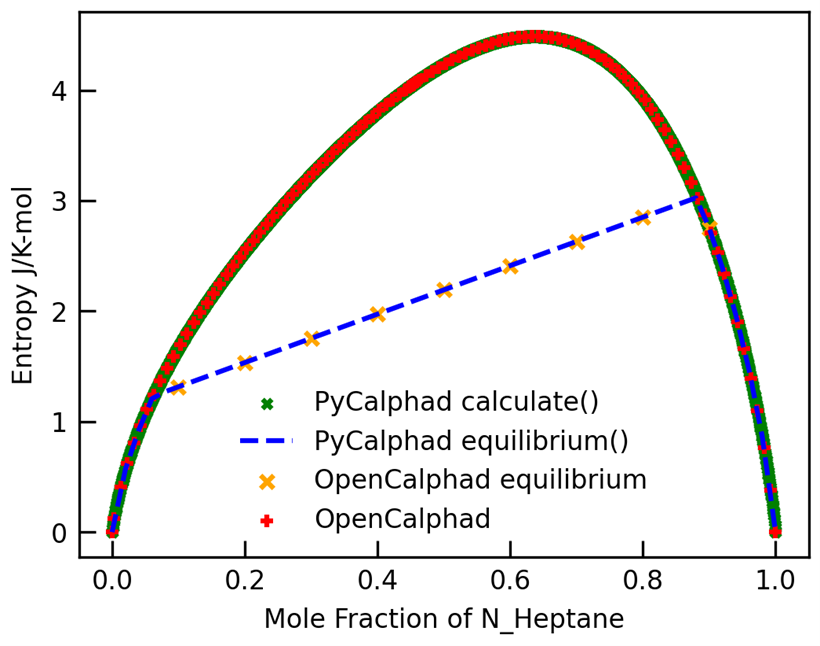
\includegraphics[width=0.5\linewidth]{models/Models-UQC-Entropy.png}
    \caption{Comparison of PyCalphad with OpenCalphad calculating entropy to verify the implementation of UNIQUAC. The red line represents results from OpenCalphad, the yellow $\times$ symbols represent results from OpenCalphad equilibrium calculations, the green $\times$ symbols represent results from the PyCalphad \textit{calculate()} function, and the blue line represents results from the PyCalphad \textit{equilibrium()} function.}
    \label{models:fig:UQCS}
\end{figure}

\begin{table}[H]
    \centering
    \caption{The entropy value calculated from PyCalphad compared to values from OpenCalphad at four different compositions.}
    \begin{tabular}{>{\raggedright\arraybackslash}m{1.5cm}>{\raggedright\arraybackslash}m{3.5cm}>{\raggedright\arraybackslash}m{3.5cm}>{\raggedright\arraybackslash}m{3.5cm}}
    \hline
         \textbf{$x_i$}&\textbf{PyCalpahd}&\textbf{OpenCalphad}&\textbf{Relative difference}\\
    \hline
        0.1&1.315&1.315&0\%\\
        0.3&1.754&1.754&0\%\\
        0.5&2.192&2.192&0\%\\
        0.9&2.752&2.752&0\%\\
    \hline
    \end{tabular}
    \label{models:tab:UQCS}
\end{table}

\begin{table}[H]
    \centering
    \caption{The activity value calculated from PyCalphad compared to values from OpenCalphad at four different compositions.}
    \begin{tabular}{>{\raggedright\arraybackslash}m{1.5cm}>{\raggedright\arraybackslash}m{3.5cm}>{\raggedright\arraybackslash}m{3.5cm}>{\raggedright\arraybackslash}m{3.5cm}}
    \hline
         \textbf{$x_i$}&\textbf{PyCalpahd}&\textbf{OpenCalphad}&\textbf{Relative difference}\\
    \hline
        0.05&0.11376&0.11376&0\%\\
        0.3&0.28710&0.28710&0\%\\
        0.5&0.47857&0.47857&0\%\\
        0.9&0.89851&0.89851&0\%\\
    \hline
    \end{tabular}
    \label{models:tab:UQCacr}
\end{table}

\begin{figure}[H]
    \centering
    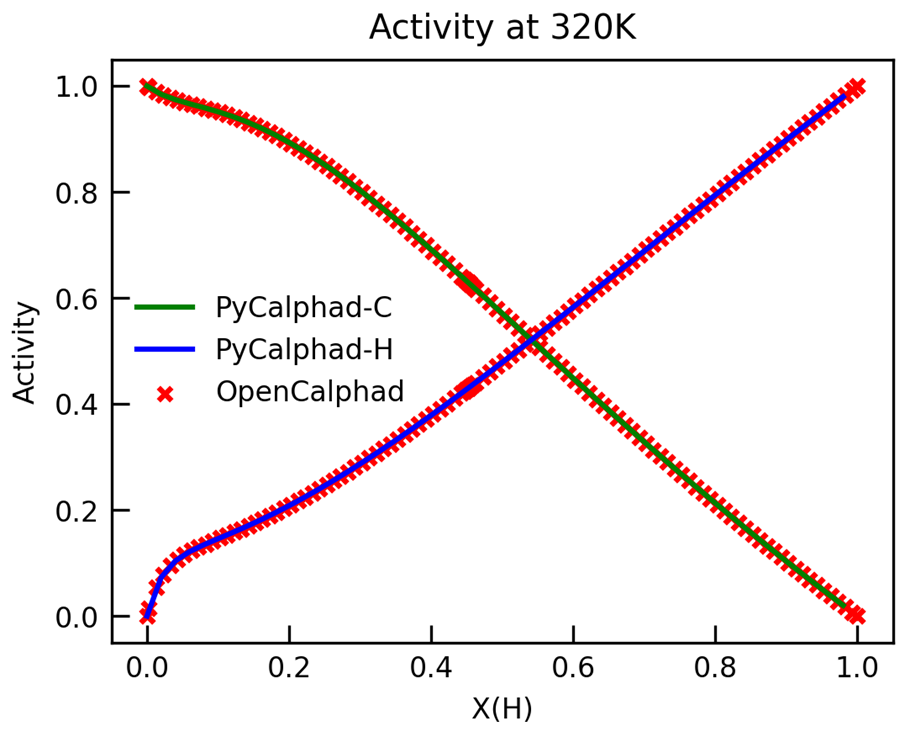
\includegraphics[width=0.5\linewidth]{models/Models-UQC-Activity.png}
    \caption{Comparison of PyCalphad with OpenCalphad calculating activity to verify the implementation of UNIQUAC. The red $\times$ symbols represent results from OpenCalphad; green and blue lines are calculated from PyCalphad.}
    \label{models:fig:UQCacr}
\end{figure}

\begin{figure}[H]
    \centering
    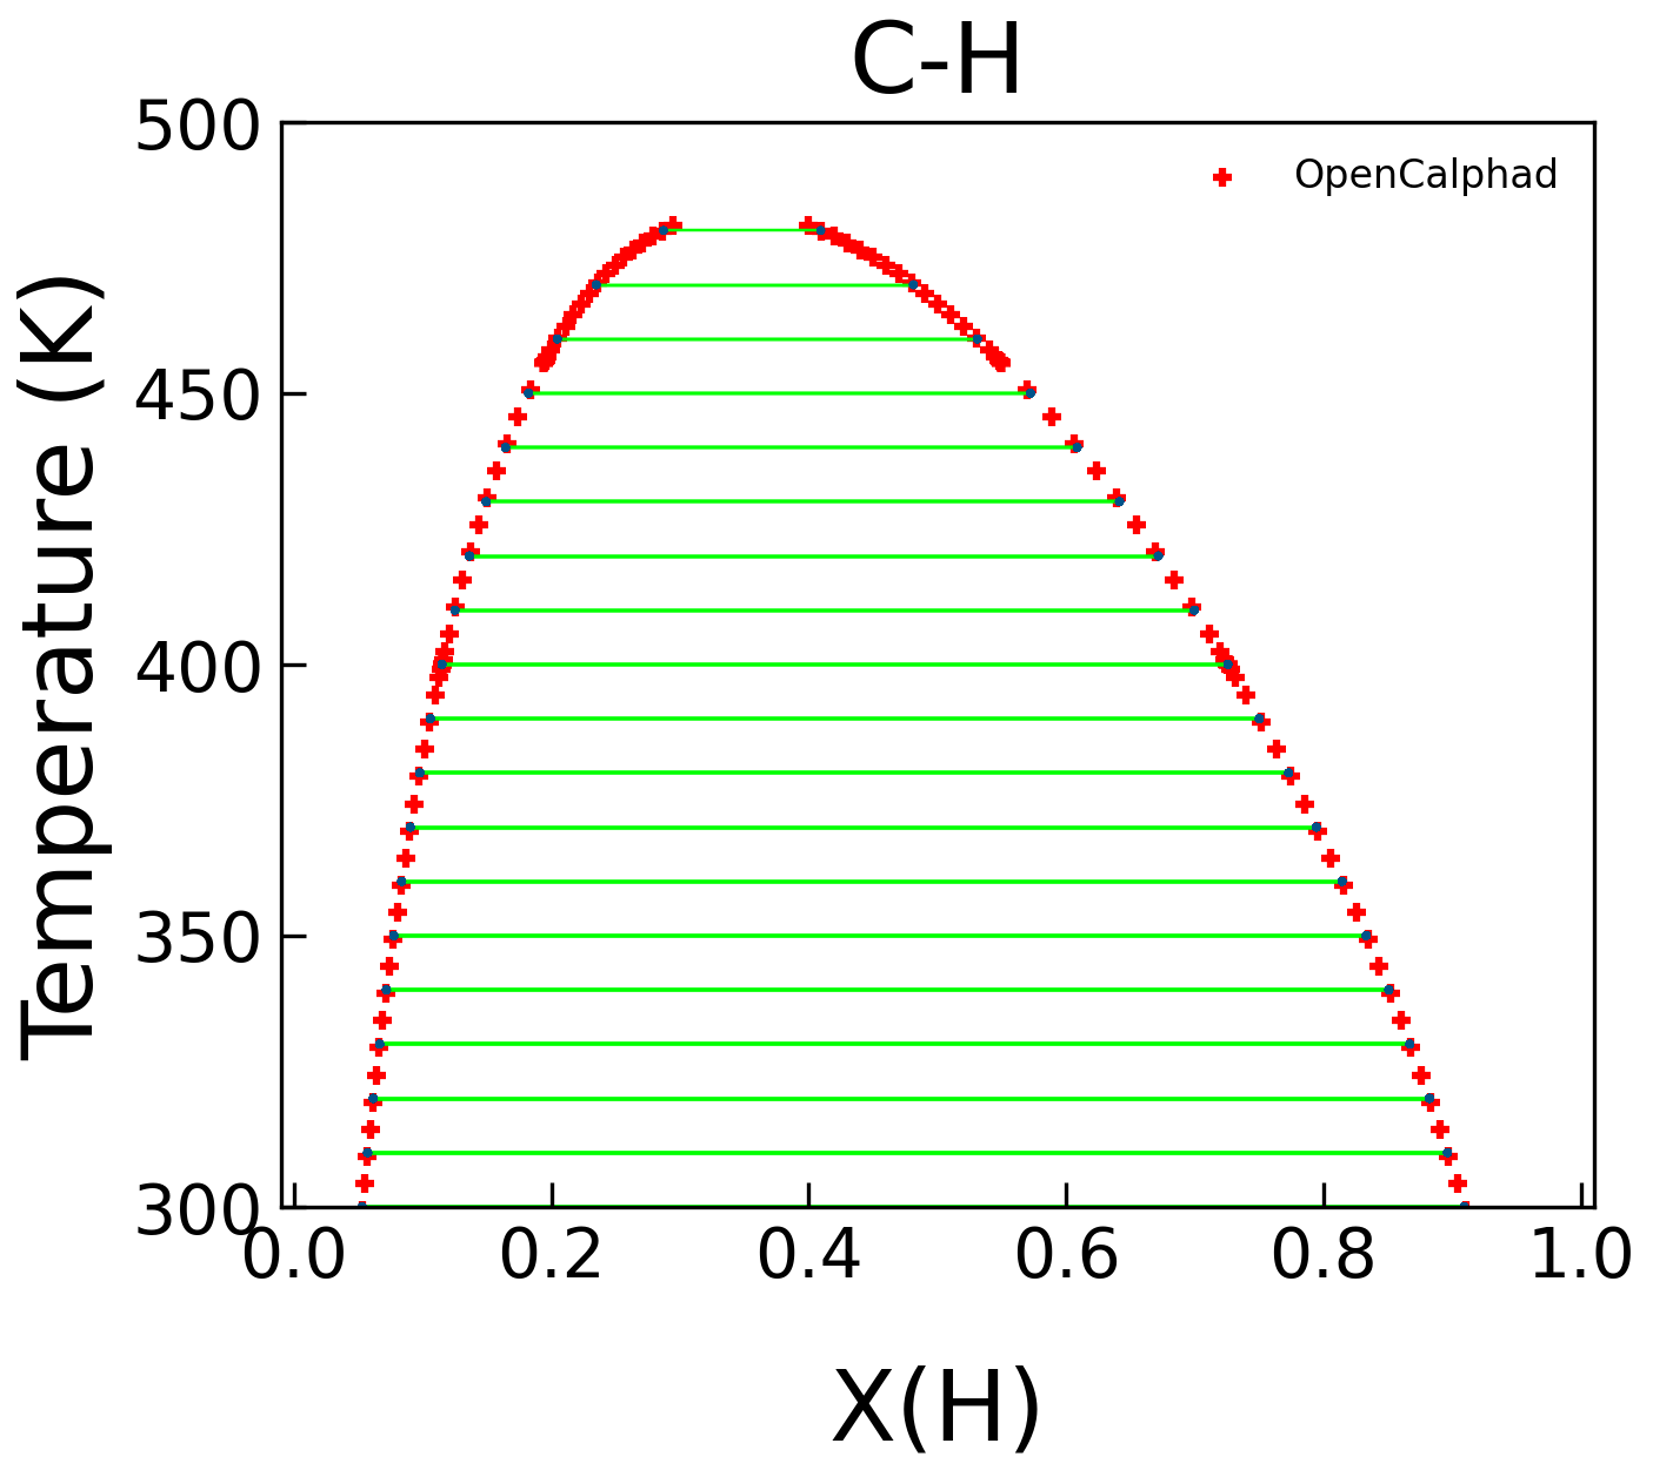
\includegraphics[width=0.5\linewidth]{models/Models-UQC-BinaryPD.png}
    \caption{Comparison of PyCalphad with OpenCalphad calculating the binary phase diagram to verify the implementation of UNIQUAC. The red $+$ symbols represent results from OpenCalphad; green lines are tie lines calculated from PyCalphad.}
    \label{models:fig:UQCBinary}
\end{figure}

\begin{figure}[H]
    \centering
    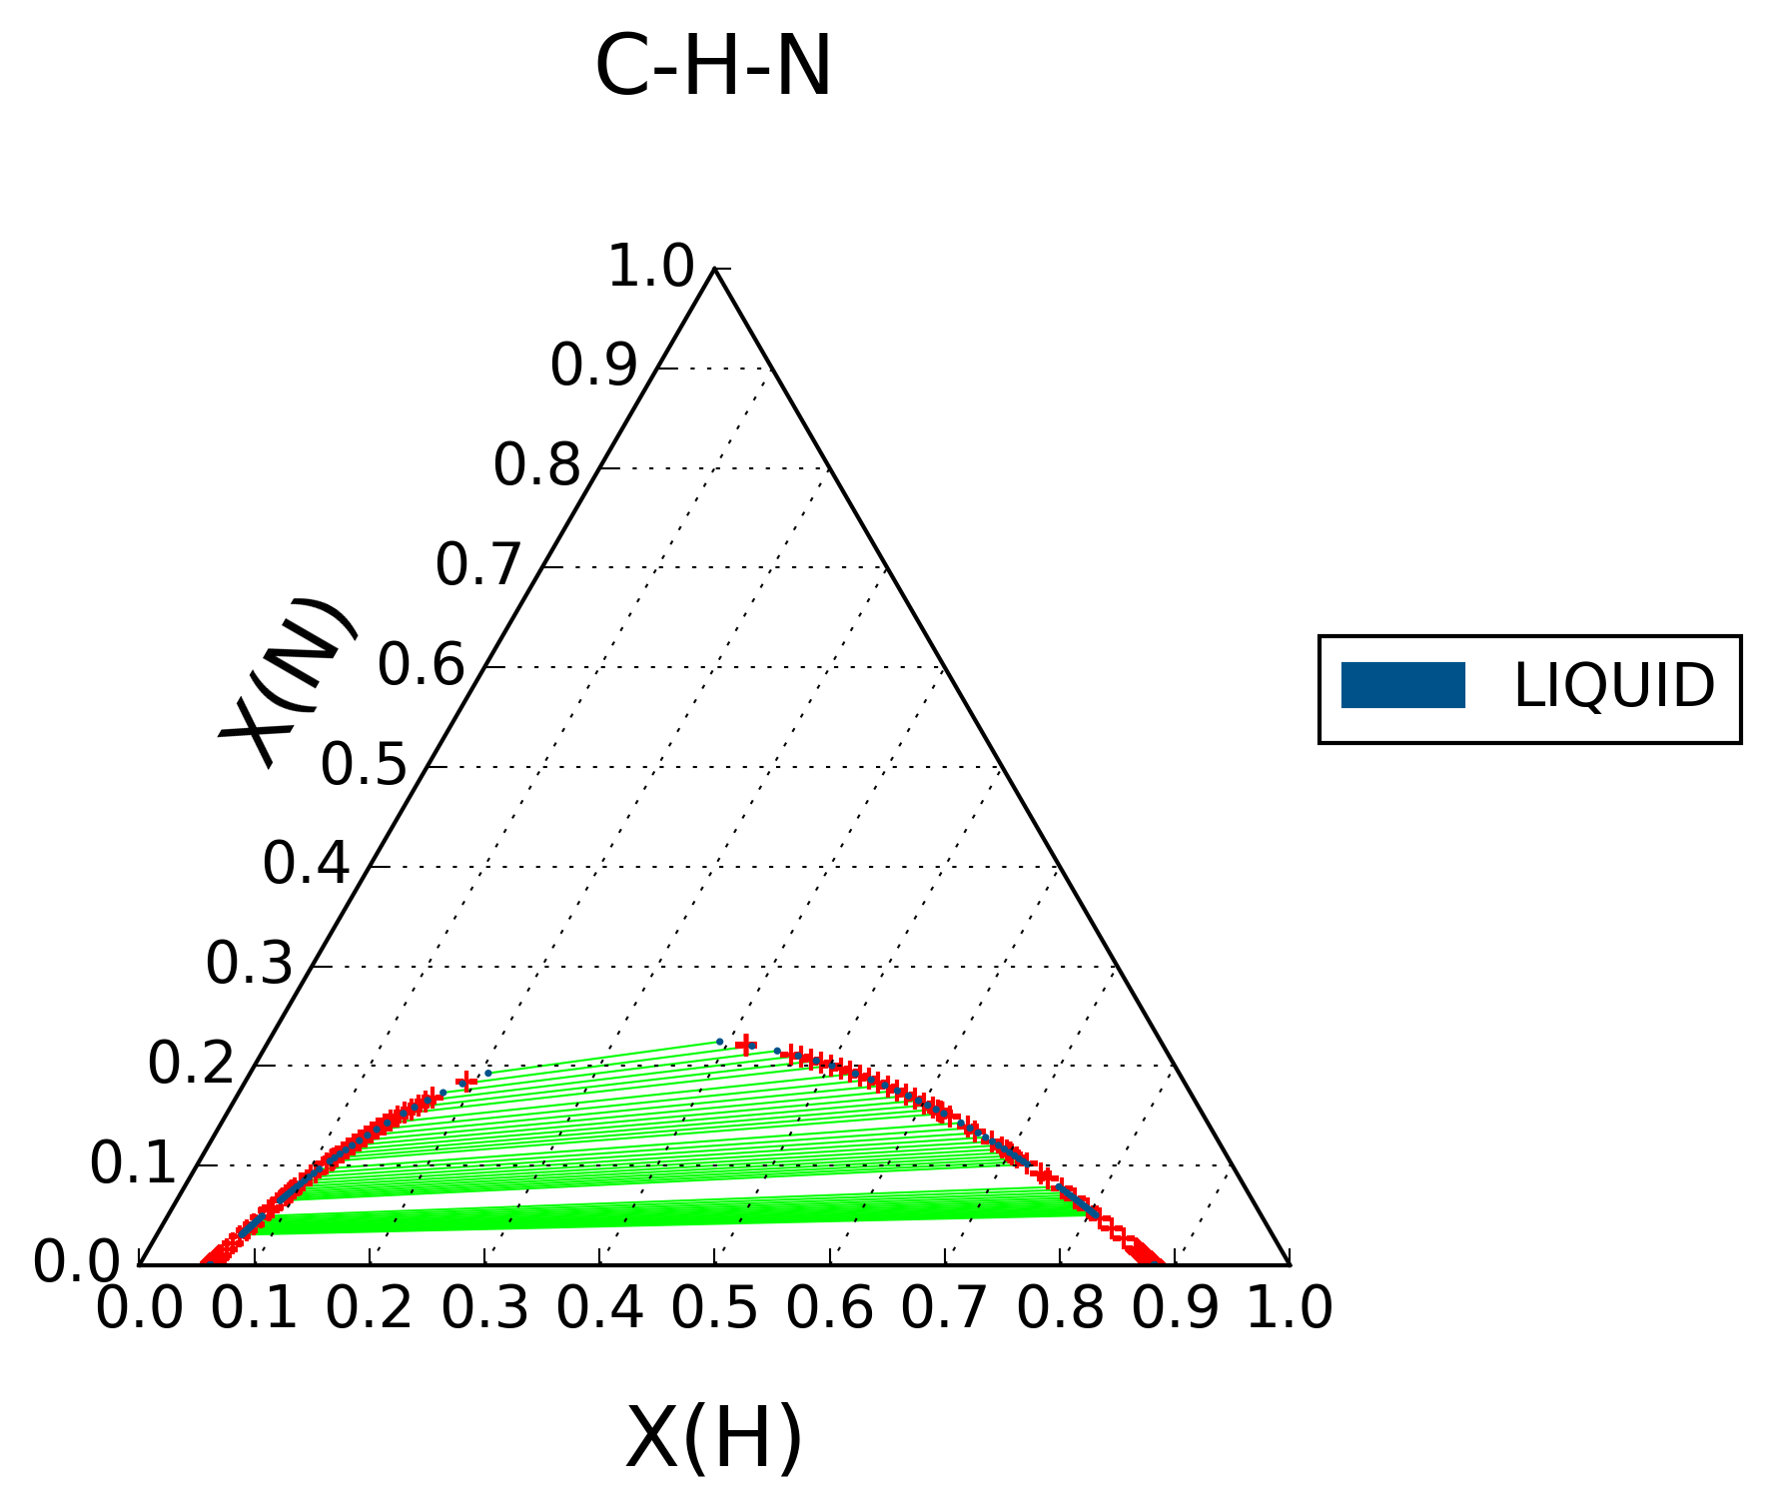
\includegraphics[width=0.5\linewidth]{models/Models-UQC-TernaryPD.png}
    \caption{Comparison of PyCalphad with OpenCalphad calculating the ternary phase diagram to verify the implementation of UNIQUAC. The red $+$ symbols represent results from OpenCalphad; green lines are tie lines calculated from PyCalphad.}
    \label{models:fig:UQCTernary}
\end{figure}

Figure \ref{models:fig:UQCBinary} and Figure \ref{models:fig:UQCTernary} shows the binary and ternary phase diagram for an artificial system modeled with UNIQUAC calculated from PyCalphad. The phase boundary matches well with phase diagram data obtained using OpenCalphad. These calculations and plots were generated using the existing functions in PyCalphad, namely \textit{equilibrium()} and \textit{eqplot()}. This alignment underscores the success of the UNIQUAC implementation in PyCalphad and demonstrates the robustness and capability of PyCalphad's existing functions for custom thermodynamic models.

\section{Custom model template generator} \label{models:sec:CMTG}
\subsection{Framework} \label{models:ssec:CMTGframework}
As illustrated in Figure \ref{models:fig:implflow}, implementing any custom model in PyCalphad requires an XML schema for the thermodynamic database and a corresponding class for PyCalphad model codes. To enhance the efficiency of adding new models and to minimize conflicts arising from format styles in PyCalphad, a custom model template generator has been developed. Figure \ref{models:fig:CMGFrame} shows the framework of this custom model template generator.

\begin{figure}[H]
    \centering
    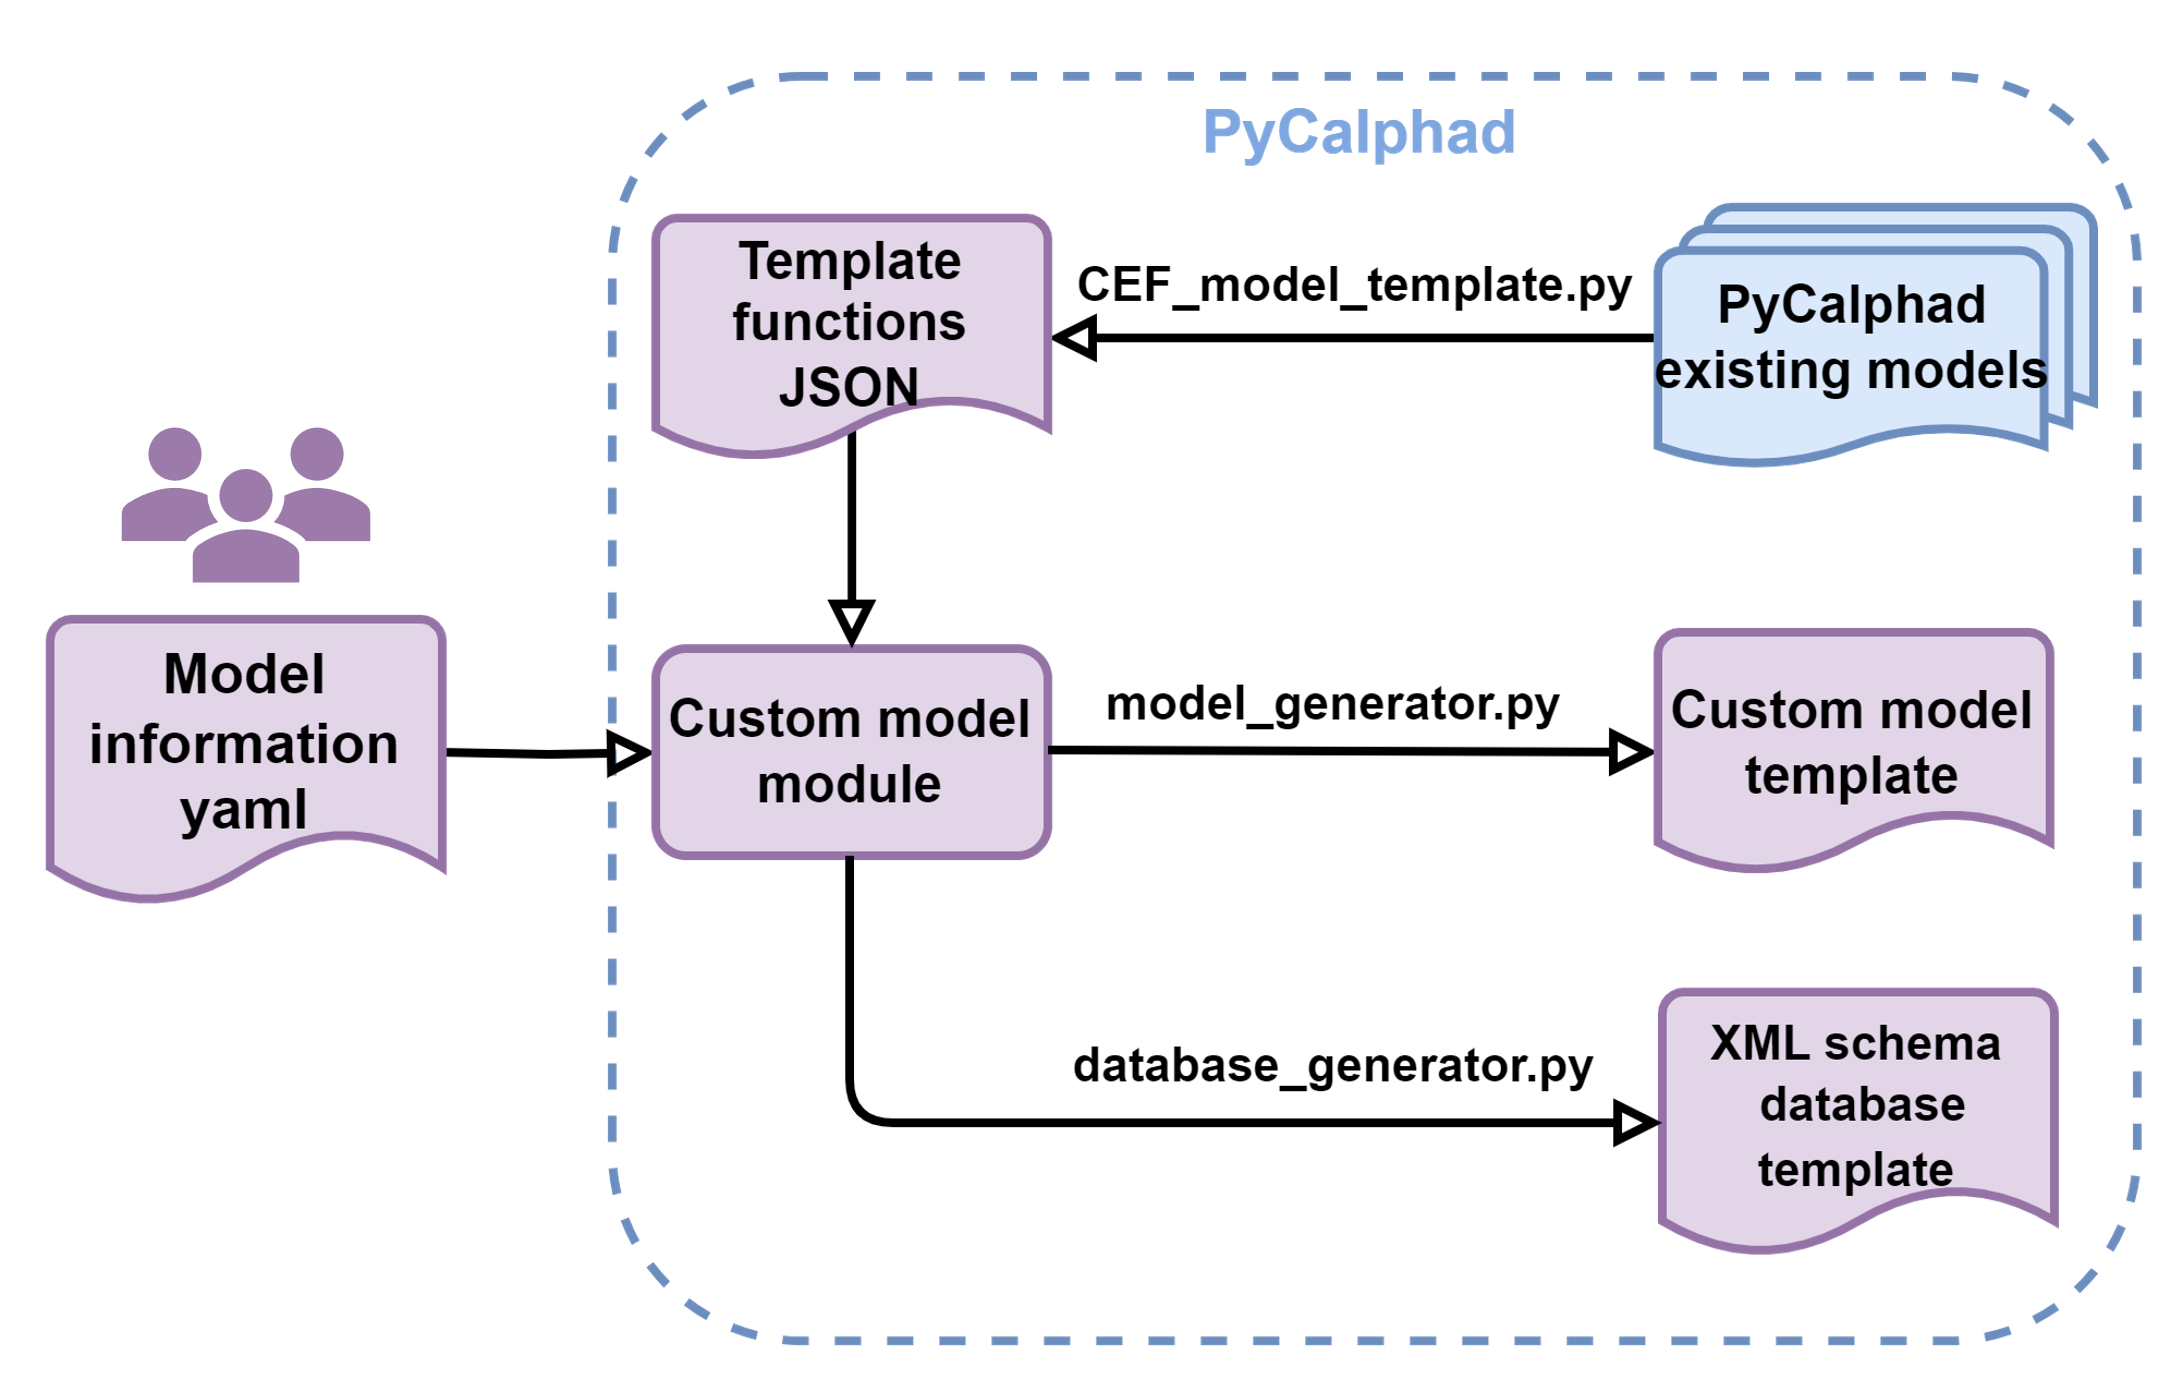
\includegraphics[width=0.8\linewidth]{models/Models-CMG-Framework.png}
    \caption{The framework of the custom model template generator.}
    \label{models:fig:CMGFrame}
\end{figure}

To use this template generator, a configuration YAML file is required to input model information, including model name, model parameters, etc. Below is an example of keywords in the model information YAML file:
\begin{minted}[xleftmargin=1\parindent, linenos=true, fontsize=\small, breaklines=true]{yaml}
    model:
      name
      energy_contributions
      basic_functions
      parameters_functions
        - parameter
          attributes
          database_keyword
          comments
      energy_functions
        - energy
          function
          comments

    database:
      name
      description
      parameters
      options
\end{minted}
There are two sections in this YAML file. The \texttt{model} key is intended to define the custom model and generate a template Python code for a PyCalphad model class. The \texttt{name} key is for input the name of the custom model. The \texttt{energy$\_$contribution}s keyword is to define what contributions to Gibbs energy are considered in the custom model. For example, in CEF, four contributions, $^{srf}G_m$, $^{cnf}S_m$, $^{xs}G_m$, and $^{phys}G_m$ are considered, while in UNIQUAC, $^{srf}G_m$, $^{cnf}S_m$, $^{cmb}G_m$, and $^{res}G_m$ are included. The \texttt{basic$\_$functions} defines some functions that can be extracted from existing models in PyCalphad to use in the custom model. The \texttt{parameters$\_$functions} is intended to define the functions for new parameters in the custom model. Information including parameter names, attributes, corresponding keywords defined in the database, and other comments for the parameter can be provided within this keyword. The \texttt{energy$\_$functions} is for the functions for energy contributions in the custom model, users are allowed to provide information including function name, function expression, and other comments for each energy contribution. The second section in the YAML file begins with the \texttt{database} key. This key is intended to define the XML database schema and generate a template XML rng file for PyCalphad-xml as shown in Section \ref{models:ssec:UNIQUACfund}. The name of the custom model can be defined with the \texttt{name} key. Comments or descriptions about the custom model, such as the full name of the model, can be input with \texttt{description}. The key \texttt{parameters} is for defining the name of new parameters in the custom model. It is corresponding with the \texttt{database$\_$keyword} value under \texttt{model: parameters$\_$functions} key. The \texttt{options} key is intended to define some optional schema for parameter structures. Options include \texttt{Exponent} and \texttt{Order}.

The major two functions in the custom model template generator are \textit{model$\_$generator()} and \textit{database$\_$generator()} as shown in Figure \ref{models:fig:CMGFrame}. In addition, there is \textit{CEF$\_$model$\_$template()} function to extract functions from existing PyCalphad models and save them into \texttt{template$\_$functions.json}. Below is the usage of these functions:
\begin{minted}[xleftmargin=1\parindent, linenos=true, fontsize=\small, breaklines=true]{python}
    configuration_file='configuration_file_name'
    output_rng_file='rng_file_name.rng'
    output_model_file='model_file_name.py'
    database_generator(configuration_file, output_rng_file)
    model_generator(configuration_file, output_model_file, print_model=True)
\end{minted}
The output of using the custom model template generator includes a \texttt{rng$\_$file$\_$name.rng} and a \texttt{model$\_$file$\_$name.py}, which users can start with for further improvement and implementation into PyCalphad.

\subsection{Application: the Peng-Robinson Euqation of State} \label{models:ssec:CMTGapp} %Add PR EOS introduction and impact
The custom model template generator has been utilized to implement the Peng-Robinson equation of state (PR EOS) \cite{peng1976new}. Developed by Peng and Robinson, this model is designed to predict the behavior of substances in gas, liquid, and supercritical fluid states \cite{peng1976new}. With more than 40 years of development, there are more than 220 modifications to the PR EOS for compounds and mixtures \cite{LopezEcheverry201739}. PR EOS is highly regarded in industrial applications, particularly in the oil, gas, and petrochemical, for its effectiveness in investigating phase equilibrium. However, there is a need to enhance the optimization process for this model, where it could greatly benefit from the capabilities offered by PyCalphad and ESPEI.

The Gibbs energy derived from PR EOS can be expressed as \cite{tang2005supercritical}:
\begin{equation} \label{models:eq:PRGm}
    G_m=\sum_i{x_i\left[^{o}G_i(T, P_0)+RT\left(\ln{x_i}+\ln{\frac{\phi_iP}{P_0}}\right)\right]}
\end{equation}
where $^{o}G_i(T, P_0)$ is the reference Gibbs energy of species $i$ at temperature T and standard state pressure $P_0$, $\phi_i$ is the fugacity coefficient of species $i$, which can be expressed as:
\begin{equation} \label{models:eq:PRphi}
    \ln{\phi_i}=\frac{b_i}{b_m}(Z-1)-\ln{(Z-B^*)}-\frac{A^*}{2B^*\sqrt{2}}\left(\frac{2\sum_jx_ja_{ij}}{a_m}-\frac{b_i}{b_m}\right)\ln{\left(\frac{Z+(1+\sqrt{2}B^*)}{Z+(1-\sqrt{2}B^*)}\right)}
\end{equation}
\begin{equation} \label{models:eq:PRaij}
    a_{ij}=(a_ia_j)^{0.5}(1-k_{ij})
\end{equation}
\begin{equation} \label{models:eq:PRam}
    a_m=\sum_i\sum_jx_ix_ja_{ij}
\end{equation} 
\begin{equation} \label{models:eq:PRAs}
    A^*=\frac{a_m(T)P}{R^2T^2}
\end{equation}
\begin{equation} \label{models:eq:PRbm}
    b_m=\sum_ix_ib_i
\end{equation} 
\begin{equation} \label{models:eq:PRBs}
    B^*=\frac{b_mP}{RT}
\end{equation}
where $a_i$ is the Peng–Robinson temperature-dependent attraction parameter of species $i$, $k_{ij}$ is binary interaction coefficient between species $i$ and $j$, $b_i$ is the Peng–Robinson temperature-independent repulsion parameter of species $i$, $a_m$ is the mixture of $a_i$ over all species, $b_m$ is the mixture of $b_i$ over all species $i$, $A^*$ is the dimensionless form of $a_m$ for a mixture, and $B^*$ is the dimensionless form of $b_m$ for a mixture. $Z$ is the compressibility factor, which can be solved by:
\begin{equation} \label{models:eq:PRZ}
    Z^3-(1-B^*)Z^2+(A^*-2B^*-3B^{*2})Z-(A^*B^*-B^{*2}-B^{*3})=0
\end{equation}

To use the PR EOS, users need to define the parameters $a_i$, $b_i$, and $k_{ij}$ in the thermodynamic database. Additionally, the parameter functions for calculating $a_{ij}$, $a_m$, $b_m$, $A^*$, $B^*$, and $Z$ are required to be defined in the model class of PR EOS. Thus, the configuration YAML file for the PR EOS can be prepared as:
\begin{minted}[xleftmargin=1\parindent, linenos=true, fontsize=\small, breaklines=true]{yaml}
model:
  name: PRModel
  energy_contributions:
    ref: reference_energy
    idmix: ideal_mixing_energy
    xsmix: excess_mixing_energy
  basic_functions: ['default']
  parameters_functions:
    - parameter: a_i
      attributes: 
        - "i: v.Species"
      database_keyword: PRMA
      comments: Peng-Robinson temperature-dependent attraction term
    - parameter: b_i
      attributes: 
        - "i: v.Species"
      database_keyword: PRMB
      comments: Peng-Robinson temperature-independent repulsion term
    - parameter: a_ij
      attributes:
        - "i: v.Species"
        - "j: v.Species"
      database_keyword: null
      comments: (a_i*a_j)^0.5(1-k_ij)
    - parameter: a_m
      attributes: null
      database_keyword: null
      comments: sum(x_i*x_j*a_ij)
    - parameter: b_m
      attributes: null
      database_keyword: null
      comments: sum(x_i*b_i)
    - parameter: A_s
      attributes: null
      database_keyword: null
      comments: (a_m*P)/(R^2*T^2)
    - parameter: B_s
      attributes: null
      database_keyword: null
      comments: (b_m*P)/(R*T)
    - parameter: Z
      attributes: null
      database_keyword: null
      comments: solve from A_s and B_s
  energy_functions:
    - energy: reference_energy
      function: CEF-default
      comments: null
    - energy: ideal_mixing_energy
      function: CEF-default
      comments: null
    - energy: excess_mixing_energy
      function: null
      comments: fugacity

database:
  name: PRModel
  description: Peng-Robinson model
  parameters:
    PRMA: Peng-Robinson temperature-dependent attraction term
    PRMB: Peng-Robinson temperature-independent repulsion term
    PRMK: Peng-Robinson interaction parameter
  options:
   - Exponents
\end{minted}
The XML rng file for PR EOS can be obtained by running the template generator functions:
\begin{minted}[xleftmargin=1\parindent, linenos=true, fontsize=\small, breaklines=true]{python}
    configuration_file='PR_Model.yaml'
    output_file='PR_schema.rng'
    database_generator(configuration_file, output_file)
\end{minted}
The partial output of the XML rng file is shown as follows:
\begin{minted}[xleftmargin=1\parindent, linenos=true, fontsize=\small, breaklines=true]{xml}
<?xml version='1.0' encoding='utf-8'?>
...
    <include href="core.rng"/>
    <define name="PRModelConstituentArray">
        <element name="ConstituentArray">
           ...
        </element>
    </define>
    <define name="PRModel.model" combine="choice">
        <element name="Model">
            <attribute name="type">
                <a:documentation>Peng-Robinson model</a:documentation>
                <value>PRModel</value>
            </attribute>
            <interleave>
                <ref name="PRModelConstituentArray"/>
                ...
            </interleave>
        </element>
        <zeroOrMore>
            <element name="Parameter">
                <attribute name="type">
                    <choice>
                        <value>PRMA</value>
                        <a:documentation>Peng-Robinson temperature-dependent attraction term</a:documentation>
                        <value>PRMB</value>
                        <a:documentation>Peng-Robinson temperature-dependent repulson term</a:documentation>
                        <value>PRMK</value>
                        <a:documentation>Peng-Robinson interaction parameter</a:documentation>
                    </choice>
                </attribute>
                <interleave>
                    ...
                    <ref name="PRModelConstituentArray"/>
                    <optional>
                        <element name="Exponents">
                            <!--Please finalize details of this optional adding.-->
                        </element>
                    </optional>
                </interleave>
            </element>
        </zeroOrMore>
    </define>
    <!--Please modify database.rng and parser.py in pycalphad-xml-->
</grammar>
\end{minted}
The Python class file for PR EOS can be obtained by running the template generator functions:
\begin{minted}[xleftmargin=1\parindent, linenos=true, fontsize=\small, breaklines=true]{python}
    configuration_file='PR_Model.yaml'
    output_file='PR_model.py'
    model_generator(configuration_file, output_file, print_model=True)
\end{minted}
The partial output of the PR EOS model class is shown as below:
\begin{minted}[xleftmargin=1\parindent, linenos=true, fontsize=\small, breaklines=true]{python}
class PRModel(Model):
    contributions = [
	("ref", "reference_energy"),
	("idmix", "ideal_mixing_energy"),
	("xsmix", "excess_mixing_energy")
	]
    ...
    def a_i(self, dbe, i: v.Species):
    	param_query=(
			(where("phase_name") == self.phase_name) & \
			(where("parameter_type") == "PRMA") & \
			(where("constituent_array").test(self._array_validity))
		)
		params = dbe._parameters.search(param_query)
    	#Peng-Robinson temperature-dependent attraction term
    	return a_i
    def b_i(self, dbe, i: v.Species):
    	param_query=(
			(where("phase_name") == self.phase_name) & \
			(where("parameter_type") == "PRMB") & \
			(where("constituent_array").test(self._array_validity))
		)
		params = dbe._parameters.search(param_query)
    	#Peng-Robinson temperature-dependent repulsion term
    	return b_i
    def a_ij(self, dbe, i: v.Species, j: v.Species):
    	#(a_i*a_j)^0.5(1-k_ij)
    	return a_ij
    def a_m(self, dbe):
    	#sum(x_i*x_j*a_ij)
    	return a_m
    def b_m(self, dbe):
    	#sum(x_i*b_i)
    	return b_m
    def A_s(self, dbe):
    	#(a_m*P)/(R^2*T^2)
    	return A_s
    def B_s(self, dbe):
    	#(b_m*P)/(R*T)
    	return B_s
    def Z(self, dbe):
    	#solve from A_s and B_s
    	return Z    
    def reference_energy(self, be):
        ...
        return pure_energy_term / self._site_ratio_normalization

    def ideal_mixing_energy(self, be):
        ...
        return ideal_mixing_term / self._site_ratio_normalization
    #fugacity
    def excess_mixing_energy(self, dbe):
    	
	return excess_mixing_energy
\end{minted}
With these templates, users can proceed to complete the parameter functions and energy functions. An example of using this template generator for the PR EOS, along with the full version of the output, is available on GitHub.\href{https://github.com/RushiGong/CustomModelGenerator/tree/main/example}{CustomModelGenerator/example}.

\section{Summary} \label{models:sec:Summary}
In this chapter, the thermodynamic model UNIQUAC, used for describing non-ideal behavior in molecular liquids, is introduced and implemented into the open-source software PyCalphad. The implementation process involves understanding the model, expressing its Gibbs energy in CALPHAD nomenclature, and developing a Python model class in PyCalphad. Additionally, an XML thermodynamic database enables users to define new parameters for the model. The validation is performed by comparing calculation results, including Gibbs energy and its derivatives, as well as phase diagram calculations, with those from OpenCalphad. To enhance the model implementation process, a custom model template generator has been developed. The application of this template generator on the Peng-Robinson equation of state demonstrates the process of creating input configuration files, output XML schema files, and Python files. The thermodynamic models implemented in PyCalphad can leverage existing features such as Gibbs energy minimization, feature customization, incorporation of ESPEI for parameter optimization, and uncertainty quantification. This advancement presents new opportunities for the broader community in thermodynamic modeling. It streamlines the process of implementing new models, increases the accessibility and usability of complex thermodynamic calculations, and promotes innovation within the broad community.

\chapter{Conclusion} \label{chap:conclusion}

\section{Conclusions} \label{conclusion:sec:conclusions}

\section{Impact} \label{conclusion:sec:impact}

\section{Future work} \label{conclusion:sec:future}


% Appendices

%\begin{appendices}

%\mypart{Appendices}

%\chapter{Supplementary Discussions} \label{chap:supdiscussions}

\section{Machine Learning Overview towards Atomistic Materials Science} \label{sipfenn:appedix1}
The class of deep learning methods has been remarkably successful in recent years in applications ranging from computer vision to natural language processing and simulations of quantum systems \cite{lecun2015deep,silver2016mastering,devlin2018bert,carleo2017solving}. Although deep neural networks have existed for a long time \cite{rosenblatt1958perceptron}, and had been successfully applied to computer vision tasks \cite{lecun1995comparison,lecun1990handwritten,lecun1998gradient}, a major breakthrough was the \texttt{AlexNet} network \cite{krizhevsky2012imagenet}, which dramatically improved the accuracy achievable on large-scale image classification. Following this success, deep neural networks have been very intensively studied and applied to a variety of problems \cite{lecun2015deep,silver2016mastering,devlin2018bert}. Deep neural networks are particularly effective when applied to regression problems, where one is learning a functional relationship between a feature and a prediction. For many problems, deep neural networks are able to achieve significantly better performance than competing machine learning methods, due to their ability to learn more complex relationships. With materials science being a field where many complex dependencies are intertwined, it is to be expected that this superior pattern recognition can carry over to the improvement in the prediction of material properties.

\subsection{Regression Problem Formulation and Artificial Neural Networks}
\label{sipfenn:ssec:regressionformulation}

The general formulation of a regression problem in statistical machine learning is to find a function $f:X\rightarrow Y$ which minimizes the risk \cite{vapnik1999overview}, also known as loss or expected error.
\begin{equation}\label{sipfenn:true_risk_app}
    R(f) = \mathbb{E}_{x,y\sim \mathcal{P}} l(y,f(x)).
\end{equation}
Here $X$ denotes a space of input features, $Y$ denotes an output space, the expectation above is taken over an unknown distribution $\mathcal{P}$ on $X\times Y$ (representing the true relationship between inputs and outputs), and $l$ is a given loss function. The goal is to find a function $f$ which accurately predicts the (potentially random) output $y$ given an input $x$.

In the present work, $x\in X$ represents the input features (descriptor) characteristic of the material, and $y\in Y$ represents the formation energy. The distribution $\mathcal{P}$ represents the true material-property relationship between given descriptor $x$ and corresponding formation energy. This relation may not be as simple as mapping a given structure to an energy since different DFT methodologies may give different results, based on many variables, such as employed functionals. \cite{CharlesW.BauschlicherJr.1995AFunctionals, Alturk2017ComparisonMaterial} Consequently it is useful to describe this relationship via a probability distribution. Furthermore, the loss function considered in the present paper is the commonly used $\ell^1$ or absolute error (AE) loss function $l(y_1,y_2) = |y_1-y_2|$. %modified this since we are using l1, not l2 - Adam

In practice, the distribution $\mathcal{P}$ is not known. Indeed it is this relationship that one is trying to learn in the first place. Instead, what is available is data $\{(y_i,x_i)\}_{i=1}^n$, which is sampled from $\mathcal{P}$. From this one forms the empirical risk \cite{hastie2009elements,vapnik2013nature}
\begin{equation}\label{sipfenn:empirical_risk_app}
    L(f) = \frac{1}{n}\displaystyle\sum_{i=1}^n l(y_i, f(x_i)),
\end{equation}
and seeks a function $f$ which minimizes the empirical risk, also known as the training error.

In addition, one must specify the type of relationship that is expected to be found between the inputs $x_i\in X$ and the predictions $y_i\in Y$. This is done by restricting the function $f$ to a specific class. For instance, by restricting $f$ to be linear, which corresponds to looking for a linear relationship between $x_i$ and $y_i$, one obtains a linear regression. On the other hand, choosing $\mathcal{F}$ to be a reproducing kernel Hilbert space of functions on $X$ with the same loss $l$ one obtains the kernel ridge regression method. Thus in order to fit the model, the training error is minimized over a specific class of function $\mathcal{F}$, i.e. one solves the optimization problem
\begin{equation}\label{sipfenn:empirical_risk_min_eq}
    f^* = \arg\min_{f\in \mathcal{F}} L(f) = \arg\min_{f\in \mathcal{F}} \frac{1}{n}\displaystyle\sum_{i=1}^n l(y_i, f(x_i)).
\end{equation}

In this the class of functions $\mathcal{F}$ is chosen as the set of functions defined by a neural network architecture (schematic in Figure \ref{sipfenn:fig:nnschematic}), which leads to a deep learning method. A neural network architecture consists of a sequence of alternating linear functions and point-wise non-linear functions \cite{goodfellow2016deep}. In the figure \ref{sipfenn:fig:nnschematic} the nodes, or neurons, represent applications of a point-wise non-linear function, called an activation function, and the connections between nodes represent linear functions from the output of the nodes in one layer to the input of the next layer.

\begin{figure}[H]
    \centering
    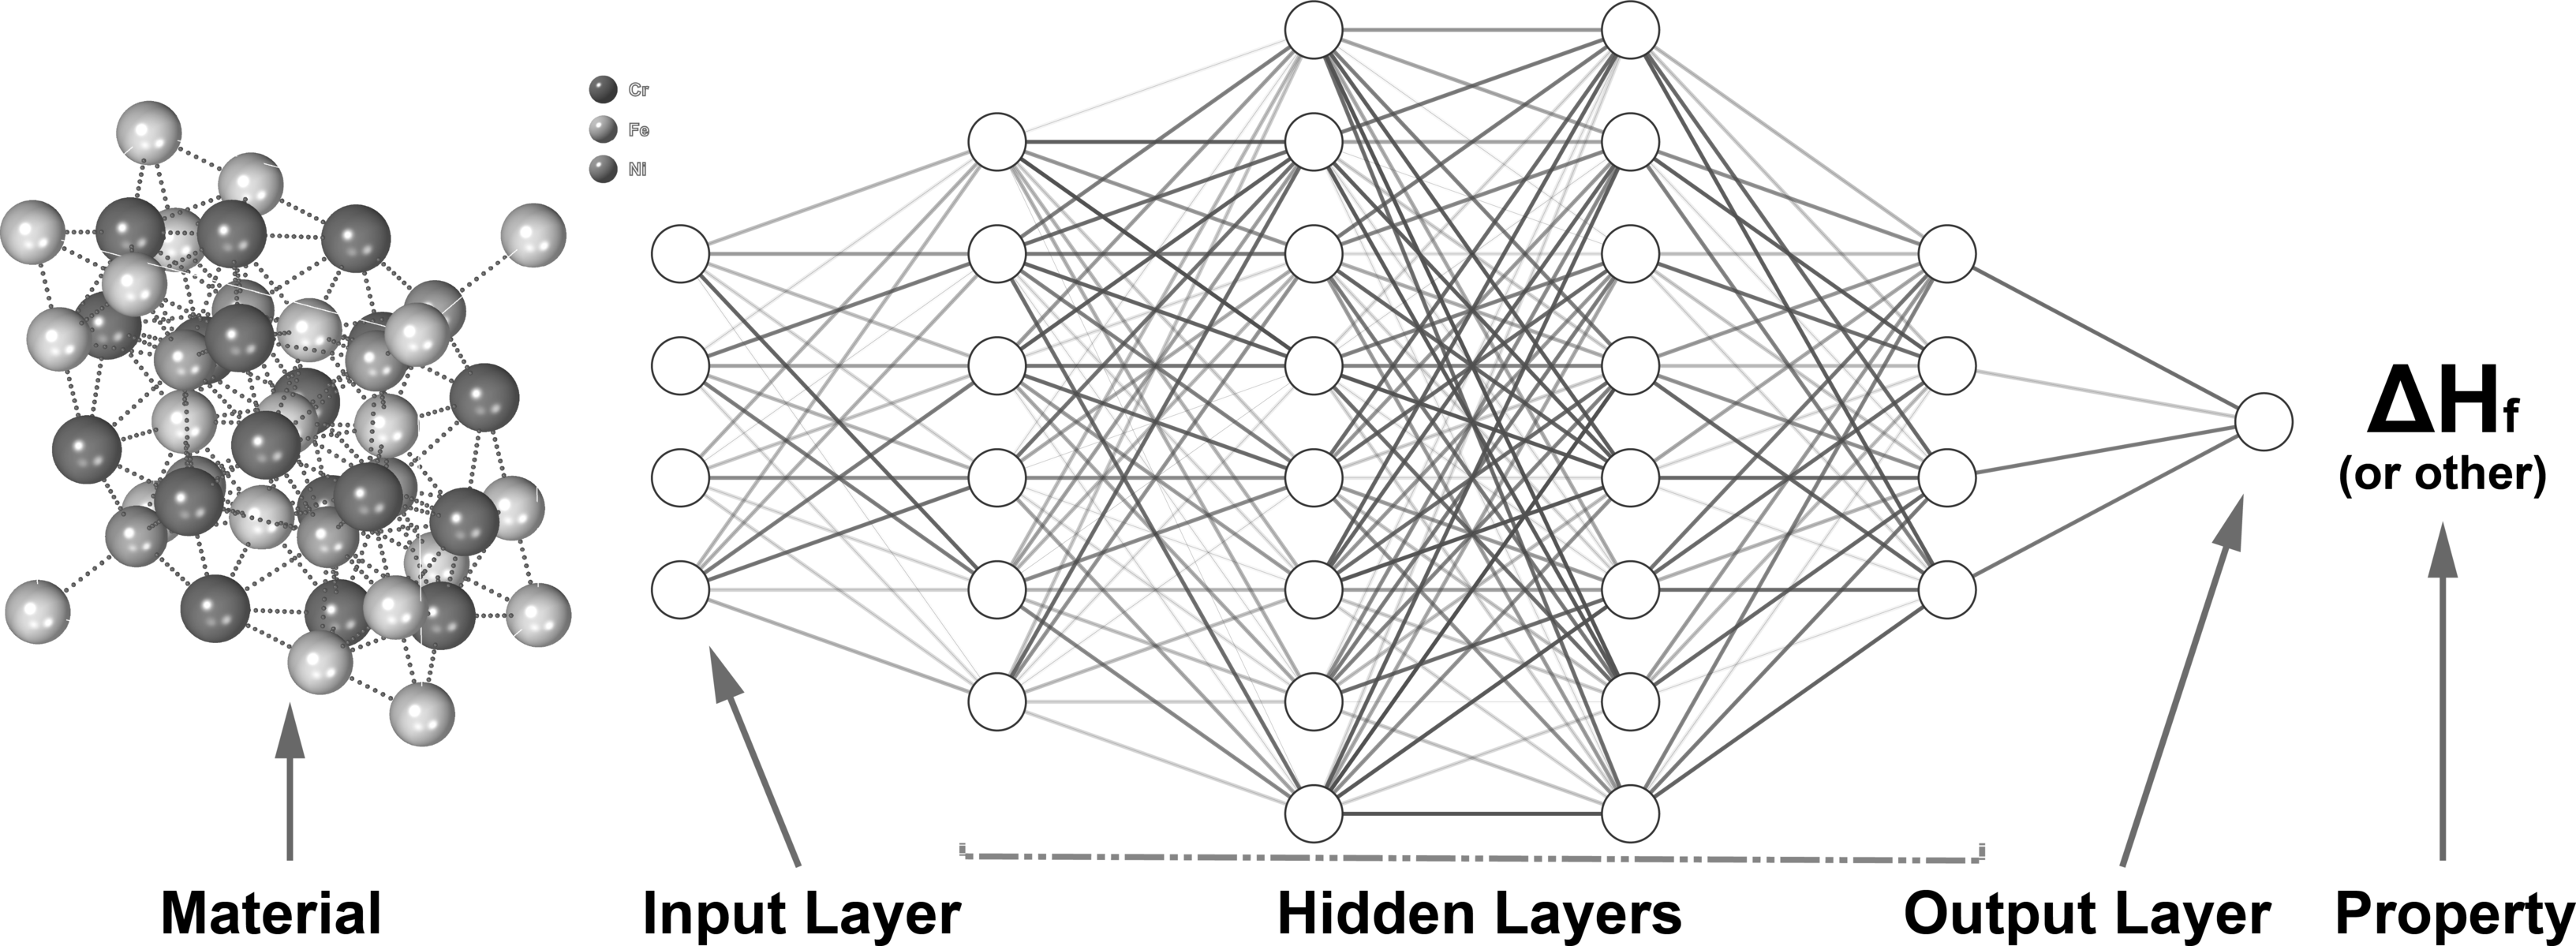
\includegraphics[width=0.85\textwidth]{sipfenn/NN_schematic.png}
    \caption{Simplified artificial neural network schematic}
    \label{sipfenn:fig:nnschematic}
\end{figure}

The class of functions represented by the neural network consists of the functions obtained by substituting different linear maps between each layer. Specifically, given weight matrices $W_1,...,W_n$ and biases $b_1,...,b_n$, which are parameters of the network, the corresponding neural network function is given by the composition

\begin{equation}
    f_{W_1,...,W_n,b_1,...,b_n}(x) = W_n\cdots\sigma(W_3\sigma(W_2\sigma(W_1x+b_1)+b_2)+b_3)\cdots + b_n
\end{equation}

where $\sigma$, called the activation function, is applied pointwise to each entry of the vector input (previous layer output). The neural network architecture is determined by the type, dimensionality, activation function $\sigma$, and arrangement of intermediate layers. This can potentially introduce some additional restrictions on the linear maps $W_i$, see for instance convolutional neural networks, where the linear maps $W_i$ are restricted to be convolutions with small kernels \cite{krizhevsky2012imagenet,lecun1995comparison,lecun1998gradient}.


Once the neural network architecture has been set, one must fit the values of the parameters $W_1,...,W_n$ and $b_1,...,b_n$ by optimizing the training loss $L$,

\begin{equation}
    \arg\min_{W_1,...,W_n,b_1,...,b_n} L(f_{W_1,...,W_n,b_1,...,b_n}).
\end{equation}

This optimization problem is typically solved using stochastic gradient descent \cite{lecun1998gradient}, or a more robust method such as ADAM \cite{kingma2014adam}, which was used in the present work. To solve the problem faster and to mitigate overfitting, which is discussed in the next sections, these methods form an estimate of the loss function gradient by considering a small subset of the data, called a batch. Each training step is done over all of the data in the batch, so parameters ($w$ and $b$) are updated based on many data points, rather than a single one. Most of the models created in the present work used a batch size of 2,048 data points.

This methodology has been successfully applied to a variety of practical machine learning problems \cite{krizhevsky2012imagenet,goodfellow2013multi,dahl2011context}. Specifically relevant to the present work, neural networks have been applied to problems in computational materials science \cite{Huang2019Machine-learningAlloys,Feng2019UsingDefects}. For example, in \cite{Huang2019Machine-learningAlloys} neural networks are used to classify the phases of high-entropy alloys. For this application, their neural network models compare favorably to other machine learning algorithms such as $k$-nearest neighbor (KNN) and support vector machines (SVM). Furthermore, in \cite{Feng2019UsingDefects} it is shown that even when training on small datasets which are typical of certain materials science problems, specifically in the prediction of solidification defects from optical microscopy data, deep neural networks can achieve better performance than other machine learning models. This is enabled by using a stacked auto-encoder (shallow neural network) to pre-train the deep neural network, whose weights are then fine-tuned on the small dataset. the present work complements these studies by applying deep neural networks to the prediction of thermodynamic quantities from atomic structure descriptors.

\subsection{Overfitting and its Mitigation}
\label{sipfenn:ssec:overfitting}

\begin{figure}[h]
    \centering
    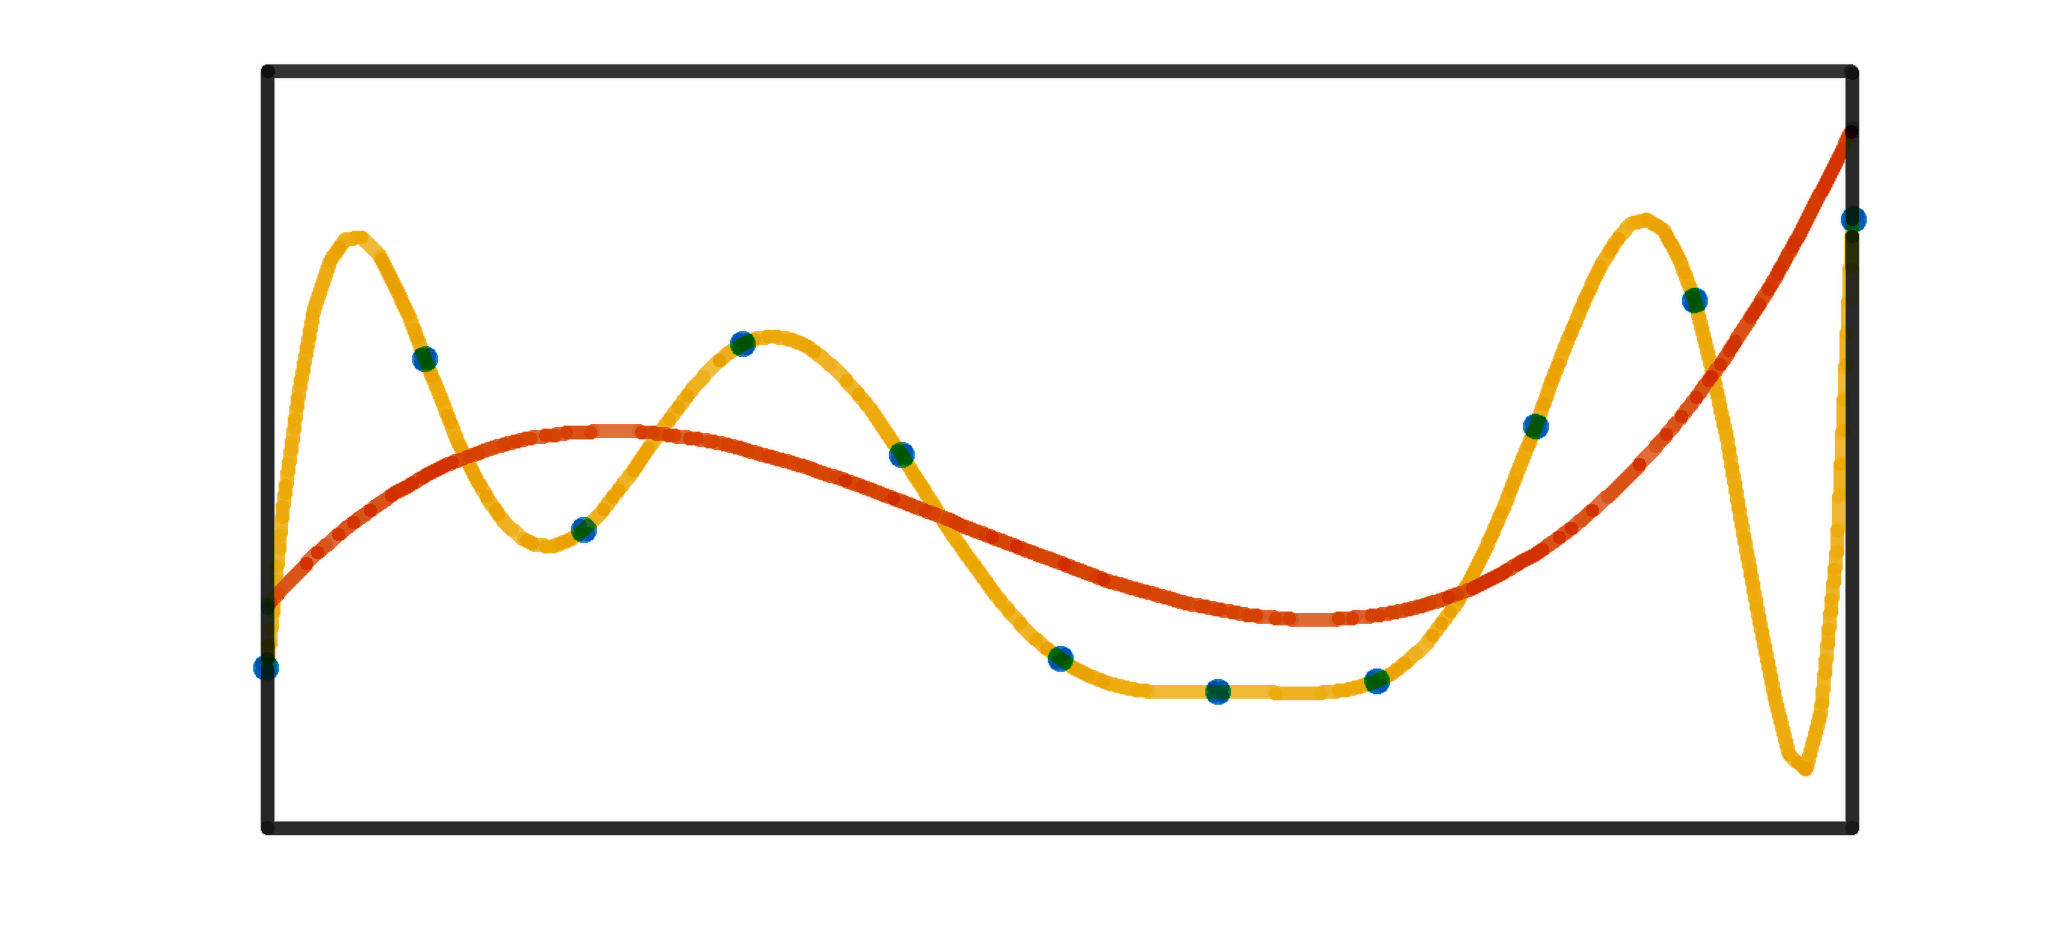
\includegraphics[width=0.5\textwidth]{sipfenn/overfitting.png}
    \caption{A schematic of overfitting. The overfit model (yellow) is too complex and memorizes the training data. This results in very low training error, but also very poor performance when predicting hidden data (test error) that follows the underlying phenomena (red).}
    \label{sipfenn:fig:overfitting}
\end{figure}

A major problem in statistical learning is avoiding overfitting \cite{hastie2009elements}, which, in simple terms, signifies that the model memorizes the training data instead of learning the true  relationship between descriptors $x$ and predictions $y$, as depicted in Figure~\ref{sipfenn:fig:overfitting}. This occurs when the class of functions $\mathcal{F}$ is too large, and at the optimal function $f^*$ in \eqref{sipfenn:empirical_risk_min_eq} the empirical \eqref{sipfenn:empirical_risk_app} and true risk \eqref{sipfenn:true_risk} diverge sharply. This results in very low training error, but poor performance on data that was not presented to the network.

Overfitting is typically detected by separating the training data into two sets, the data used in \eqref{sipfenn:empirical_risk_min_eq} to learn the function $f^*$, called the training data, and a separate set of data used to evaluate the performance of $f^*$, called the validation set. Consequently, in addition to the training loss in \eqref{sipfenn:empirical_risk_min_eq}, the validation error

\begin{equation}\label{sipfenn:validation_loss}
    L_{val} = \frac{1}{m}\displaystyle\sum_{i=1}^m l(\tilde{y}_i, f(\tilde{x}_i)),
\end{equation}

where $(\tilde{y}_i,\tilde{x}_i)$ for $i=1,...,m$ is the validation set, which was not presented to the network when adjusting its parameters, is used to detect overfitting. 
%%
The fraction of the data set aside for validation set should be large enough to be representative of the whole dataset to provide statistically significant conclusions, yet small enough so that knowledge loss in the process is minimized. In the present work, a randomly selected 15\% of every dataset has been used as validation sets for all training. This corresponded to 65,300 data points in the case of the OQDM dataset described in \ref{sipfenn:sssec:Data}.
%%

\begin{figure}{H}
    \centering
    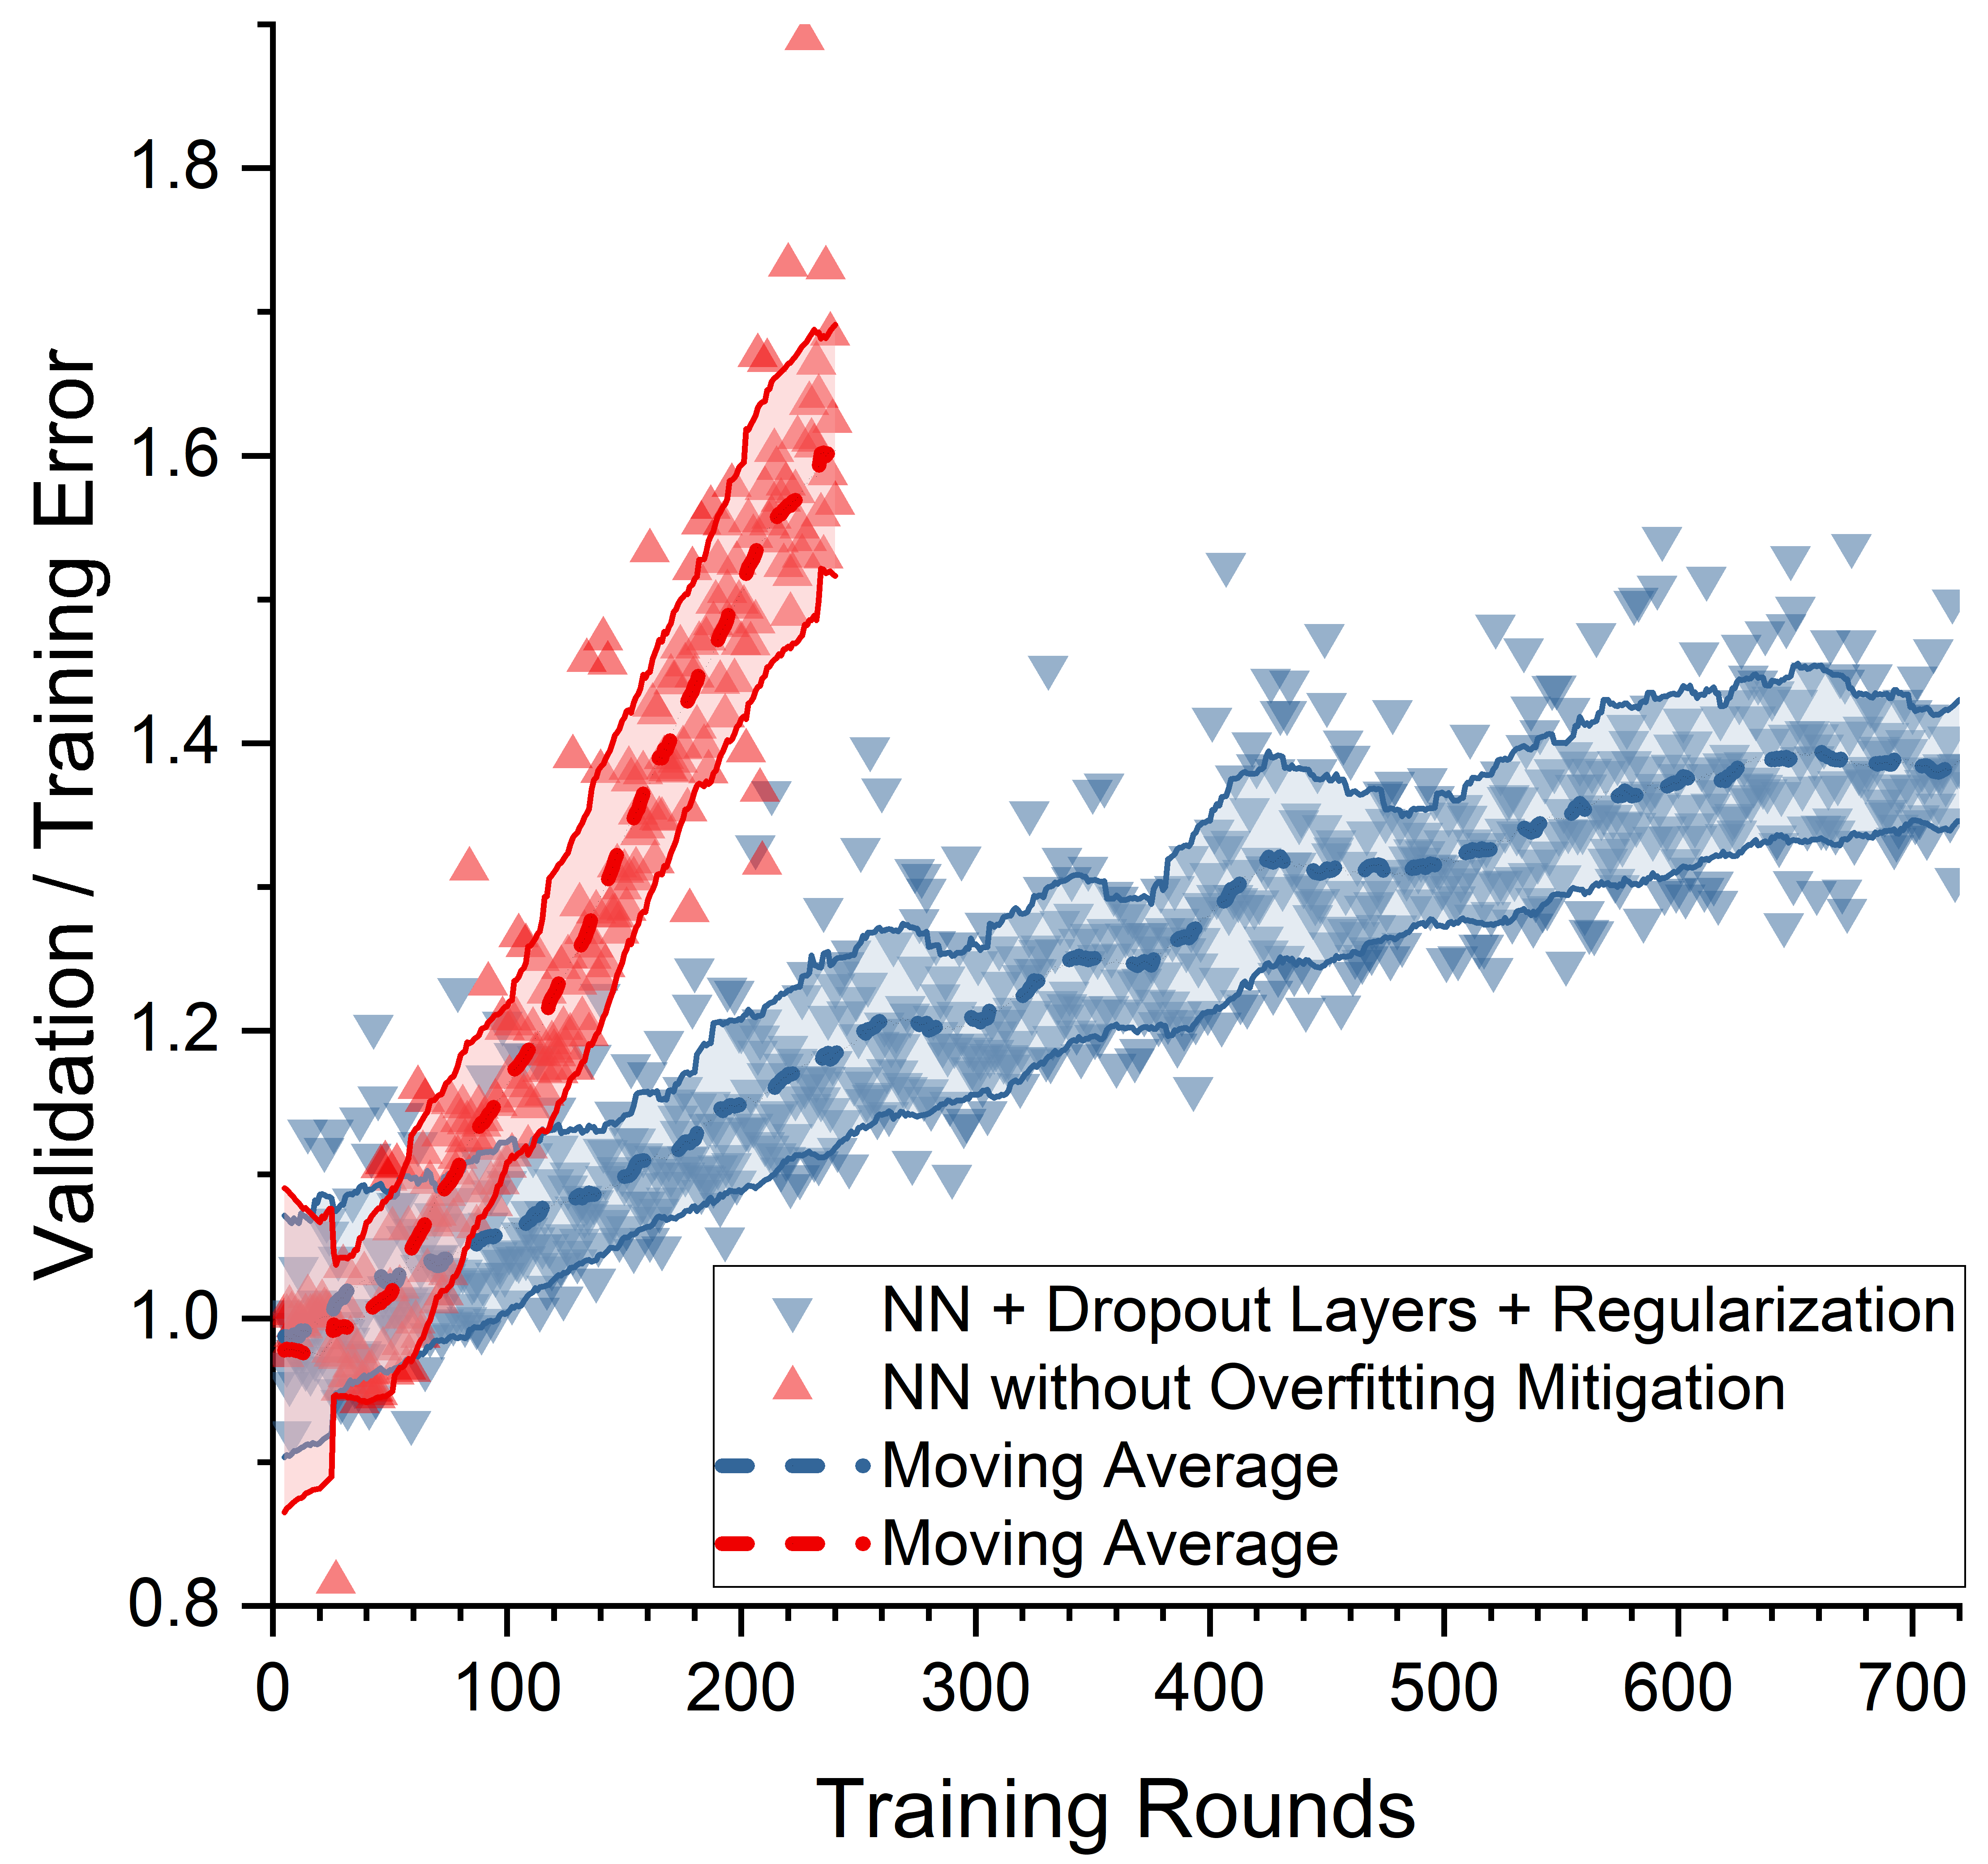
\includegraphics[width=0.65\textwidth]{sipfenn/validationtotraining_generalized.png}
    \caption{Training Loss to Validation Loss in a model that does without (NN9) and with overfitting mitigation (NN20), plotted versus training progress.}
    \label{sipfenn:fig:trainingvalidation}
\end{figure}

Typically, the validation loss will be greater than the training loss, as the validation set is not available for training. This is illustrated in Figure \ref{sipfenn:fig:trainingvalidation}, where the ratio between the validation loss \eqref{sipfenn:validation_loss} and test loss \eqref{sipfenn:empirical_risk_min_eq} during the course of two trainings of similar NN architectures on the same data with the same learning rate schedule has been plotted. This figure indicates that as the training proceeds, the gap between the training and validation errors widens and then increases. The size of this gap is an estimated measure of how much the model has overfitted to the data. In one of the models in this figure, extensive techniques to mitigate overfitting have been used, and for this model, the figure shows that the rate at which the model overfits to the data is much lower. At the same time both models exhibit similar performance on the test set.

There are numerous techniques used to prevent the issue of overfitting \cite{hastie2009elements,everitt2002cambridge}. These include utilization of a regularization term $\lambda R(\theta)$ added to the training error \eqref{sipfenn:empirical_risk_min_eq} to give the regularized empirical loss function

\begin{equation}
    f^* = \arg\min_{f\in \mathcal{F}} R_{emp}(f) + \lambda R(\theta).
\end{equation}

A standard regularizer typically added to the linear regression is the $\ell^2$-norm $R(\theta) = \|\theta\|_2^2$, which is often called Tikhonov regularization \cite{tikhonov1963solution} or ridge regression \cite{hoerl1970ridge}. The $\ell^2$-norm is also a popular regularizer in deep learning problems, where it is referred to as weight decay \cite{goodfellow2016deep}. In the context of the present work, it is implemented as a part of the training process, rather than network architecture, and causes rejection of some features in the descriptor that are not contributing to pattern recognition. Results of its implementation are shown throughout Section \ref{sipfenn:sssec:NetDesign}.

Another important method used to prevent overfitting in machine learning is the Dropout technique \cite{srivastava2014dropout}. The concept behind Dropout is to prevent neurons in the network from becoming overly dependent on the output from a specific neuron in the previous layer, often referred to as hard-wiring neuron paths. A Dropout layer, placed within a neural network, is implemented as a function operating during the training process and randomly discarding a specified fraction $p$ of previous layer outputs and multiplying the remaining values by $1/(1-p)$. This forces the pattern recognition ability to be dispersed across the network, as during evaluation of every training step, a random part of the network is acting as if it was not gone. Once the training is completed, all Dropout layers are deactivated and simply pass all information forward, so that the model returns to its deterministic character.

In the experiments performed in the present work, as later discussed in \ref{sipfenn:sssec:NetDesign}, both Dropout and weight decay were used to mitigate overfitting, with good effects shown in particular in Figure \ref{sipfenn:fig:trainingvalidation}.

Methods for avoiding overfitting typically come with one or more "hyperparameters" (i.e. parameters which control the training process) that can represent how much confidence is given to the training data versus prior knowledge. For instance, if a regularizer is used, the strength of the regularizer, $\lambda$, would be a hyperparameter. In the terms of the present work, it generally corresponds to how many features in the material descriptor can be considered non-essential to making predictions and therefore discarded systematically throughout the training. Furthermore, when using Dropout, the probability $p$ is also a hyperparameter. 

One typically trains the model on the training dataset using a number of different hyperparameters and then subsequently chooses the best set of them using the validation error. This allows the determination of hyperparameter values that are appropriate to the problem at hand. However, in order to ensure that the determined hyperparameter values are not overly specific to the validation set, the final accuracy of the model is evaluated on a test set that was not used at all during training \cite{hastie2009elements}.

\begin{figure}[H]
    \centering
    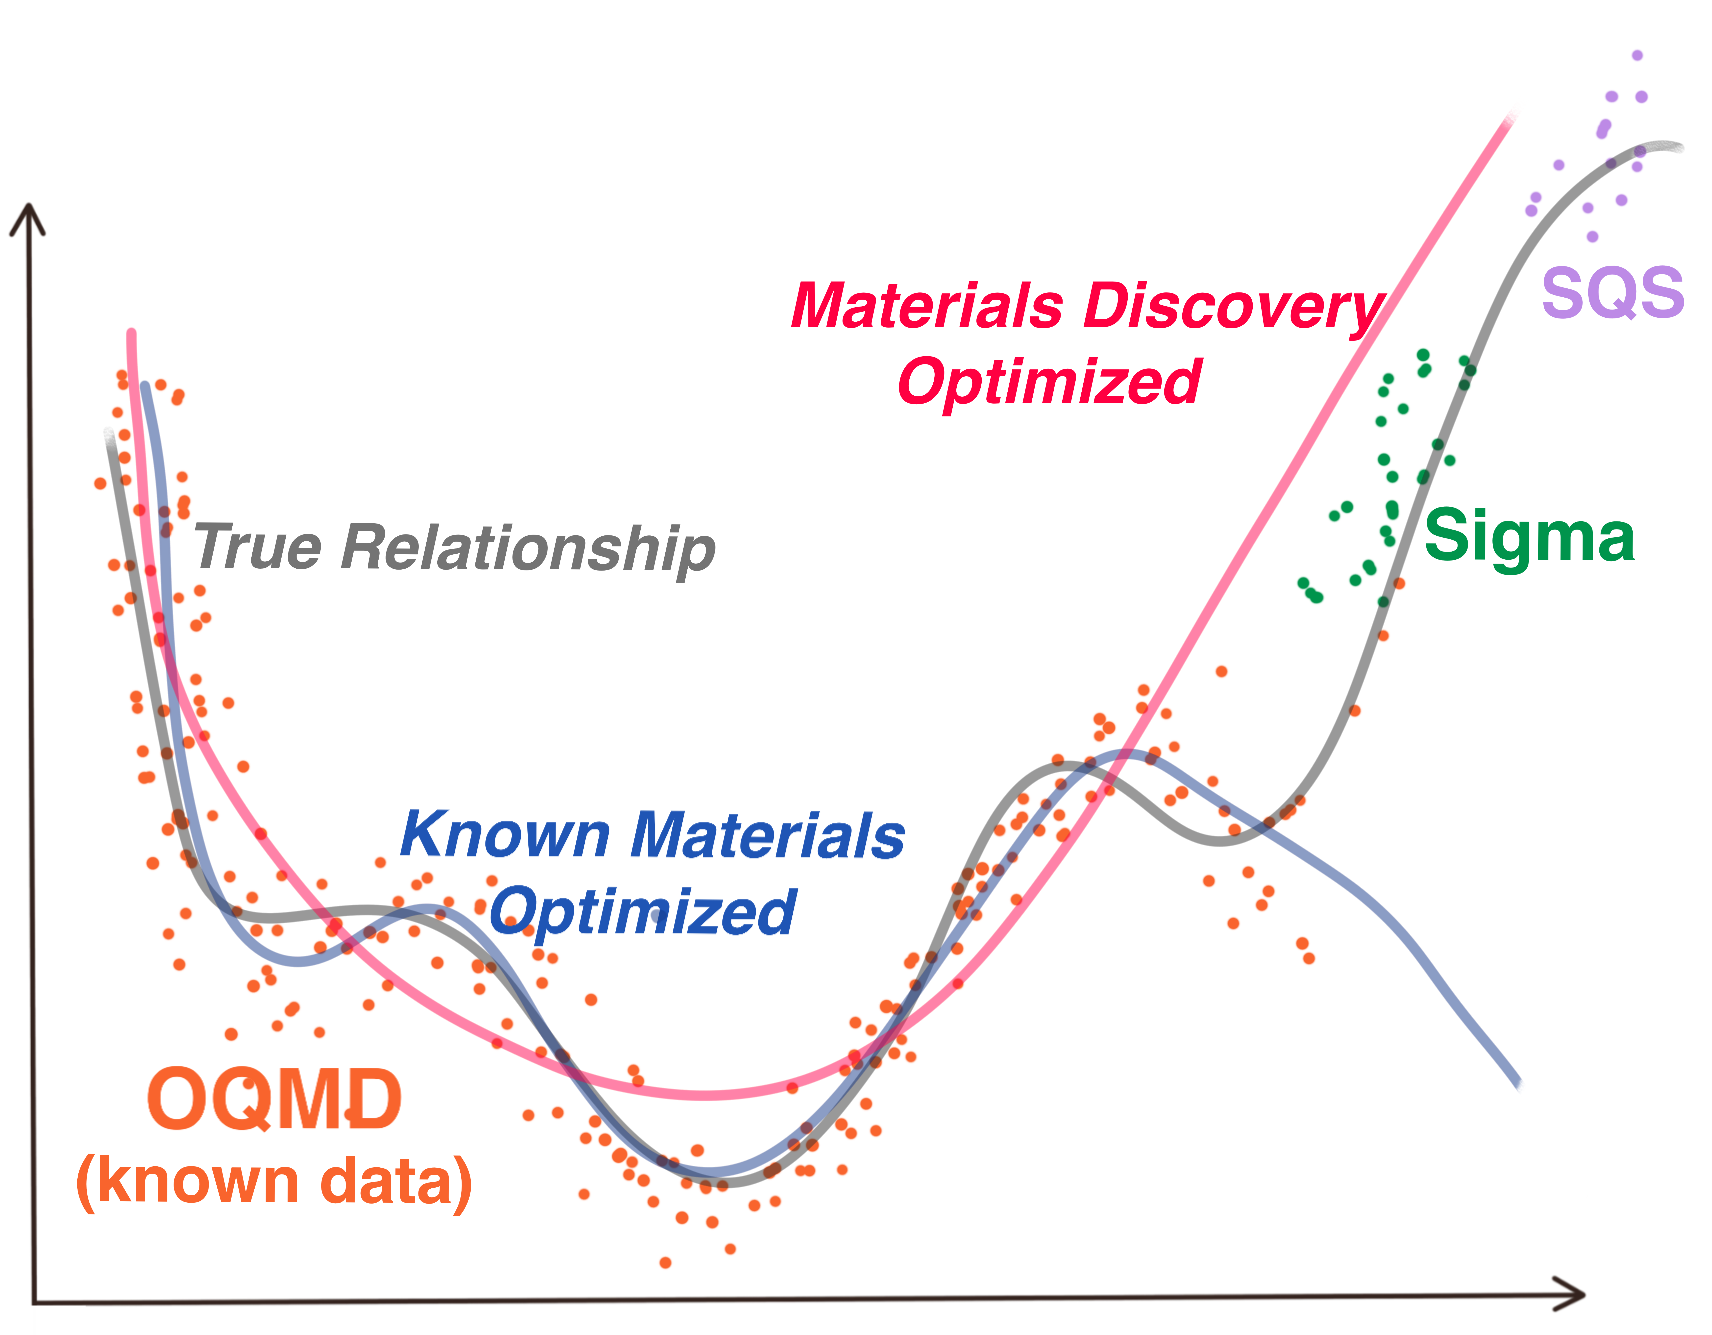
\includegraphics[width=0.7\textwidth]{sipfenn/Overfitting_discovery.png}
    \caption{A conceptual drawing depicting how overfitting mitigation effort can improve performance beyond regions with high known data density.}
    \label{sipfenn:fig:overfitting_newregions}
\end{figure}

An additional advantage of mitigating overfitting to known data can be increased performance during extrapolation, as depicted conceptually in Figure \ref{sipfenn:fig:overfitting_newregions}. This is thanks to reduced model complexity, which forces recognition of stronger and more broadly exhibited patterns rather than small deviations present in the training data, whether real or due to noise, that can significantly degrade the extrapolation capability of the ML model. It is important to recognize that cost of such model simplification is often reduced performance on previously unseen data that lays within the known region.


\subsection{Transfer Learning} \label{sipfenn:ssec:transferlearning}
Finally, one should consider the technique of transfer learning, which has been observed among deep learning models across a variety of domains \cite{tan2018survey,cirecsan2012transfer,chang2017unsupervised,george2018deep}. Transfer learning refers the to the ability of properly trained deep learning models to `transfer' their knowledge to related tasks. In the least complex approach, one does this by simply `fine-tuning' the parameters of the model using new training data (from the new task). This has to be done using a small learning rate and a small number of iterations on a loss function defined by the new training data. It has been observed that this often produces accurate results on the new task for a relatively small amount of additional data. 

As an illustrative example, in \cite{cirecsan2012transfer}, a network is first trained to recognize lower case handwritten characters. It is then shown that with minimal `fine-tuning,' such a network can be made to accurately recognize upper case characters. The same phenomenon was also observed with a network that was first trained to recognize Chinese characters. Considering that this behavior has been widely observed \cite{tan2018survey,chang2017unsupervised,george2018deep}, this shows that deep neural networks are often able to transfer knowledge between different but related tasks. 

the present work adds to this evidence by showing that a network trained on the knowledge from the OQMD database covering a broad yet limited spectrum of material, can be easily adjusted to materials outside this spectrum with very little cost relative to the initial training. Specifically, the set of all (243) Fe-Ni-Cr $\sigma$-phase endmembers, described in \ref{sipfenn:sssec:Data}, is shown in \ref{sipfenn:ssec:transferlearningresults} to require transfer of only a few examples from that set to dramatically improve model performance on the rest.

\section{Intermediate \texttt{SIPFENN} Models} \label{sipfenn:appendix2}

The neural network design process was conducted in incremental fashion, starting from a perceptron, which is the simplest type of neural network proposed by Frank Rosenblatt in 1957 \cite{Rosenblatt1957TheAutomaton}. It effectively operates as a linear function $f(\vec{d}) = A(w_1 d_1 + w_2 d_2 + ... + w_n d_n)$ where $d_i$ is i-th element of the descriptor $\vec{d}$, $w_i$ is the weight associated with it, and $A$ is an activation function that can introduce non-linearity or turn it into a classifier. Here, the popular Sigmoid activation function was used. 

The perceptron was first trained on the data from the first 5000 entries in the ICSD, to check whether the training was set up correctly. It achieved a MAE of 195 meV/atom on the test set of 230 randomly selected entries ($\approx 5\% \text{ from } 5000$). Results are shown in Figure \ref{sipfenn:fig:nn1performance}. 

\begin{figure}[H]
    \centering
    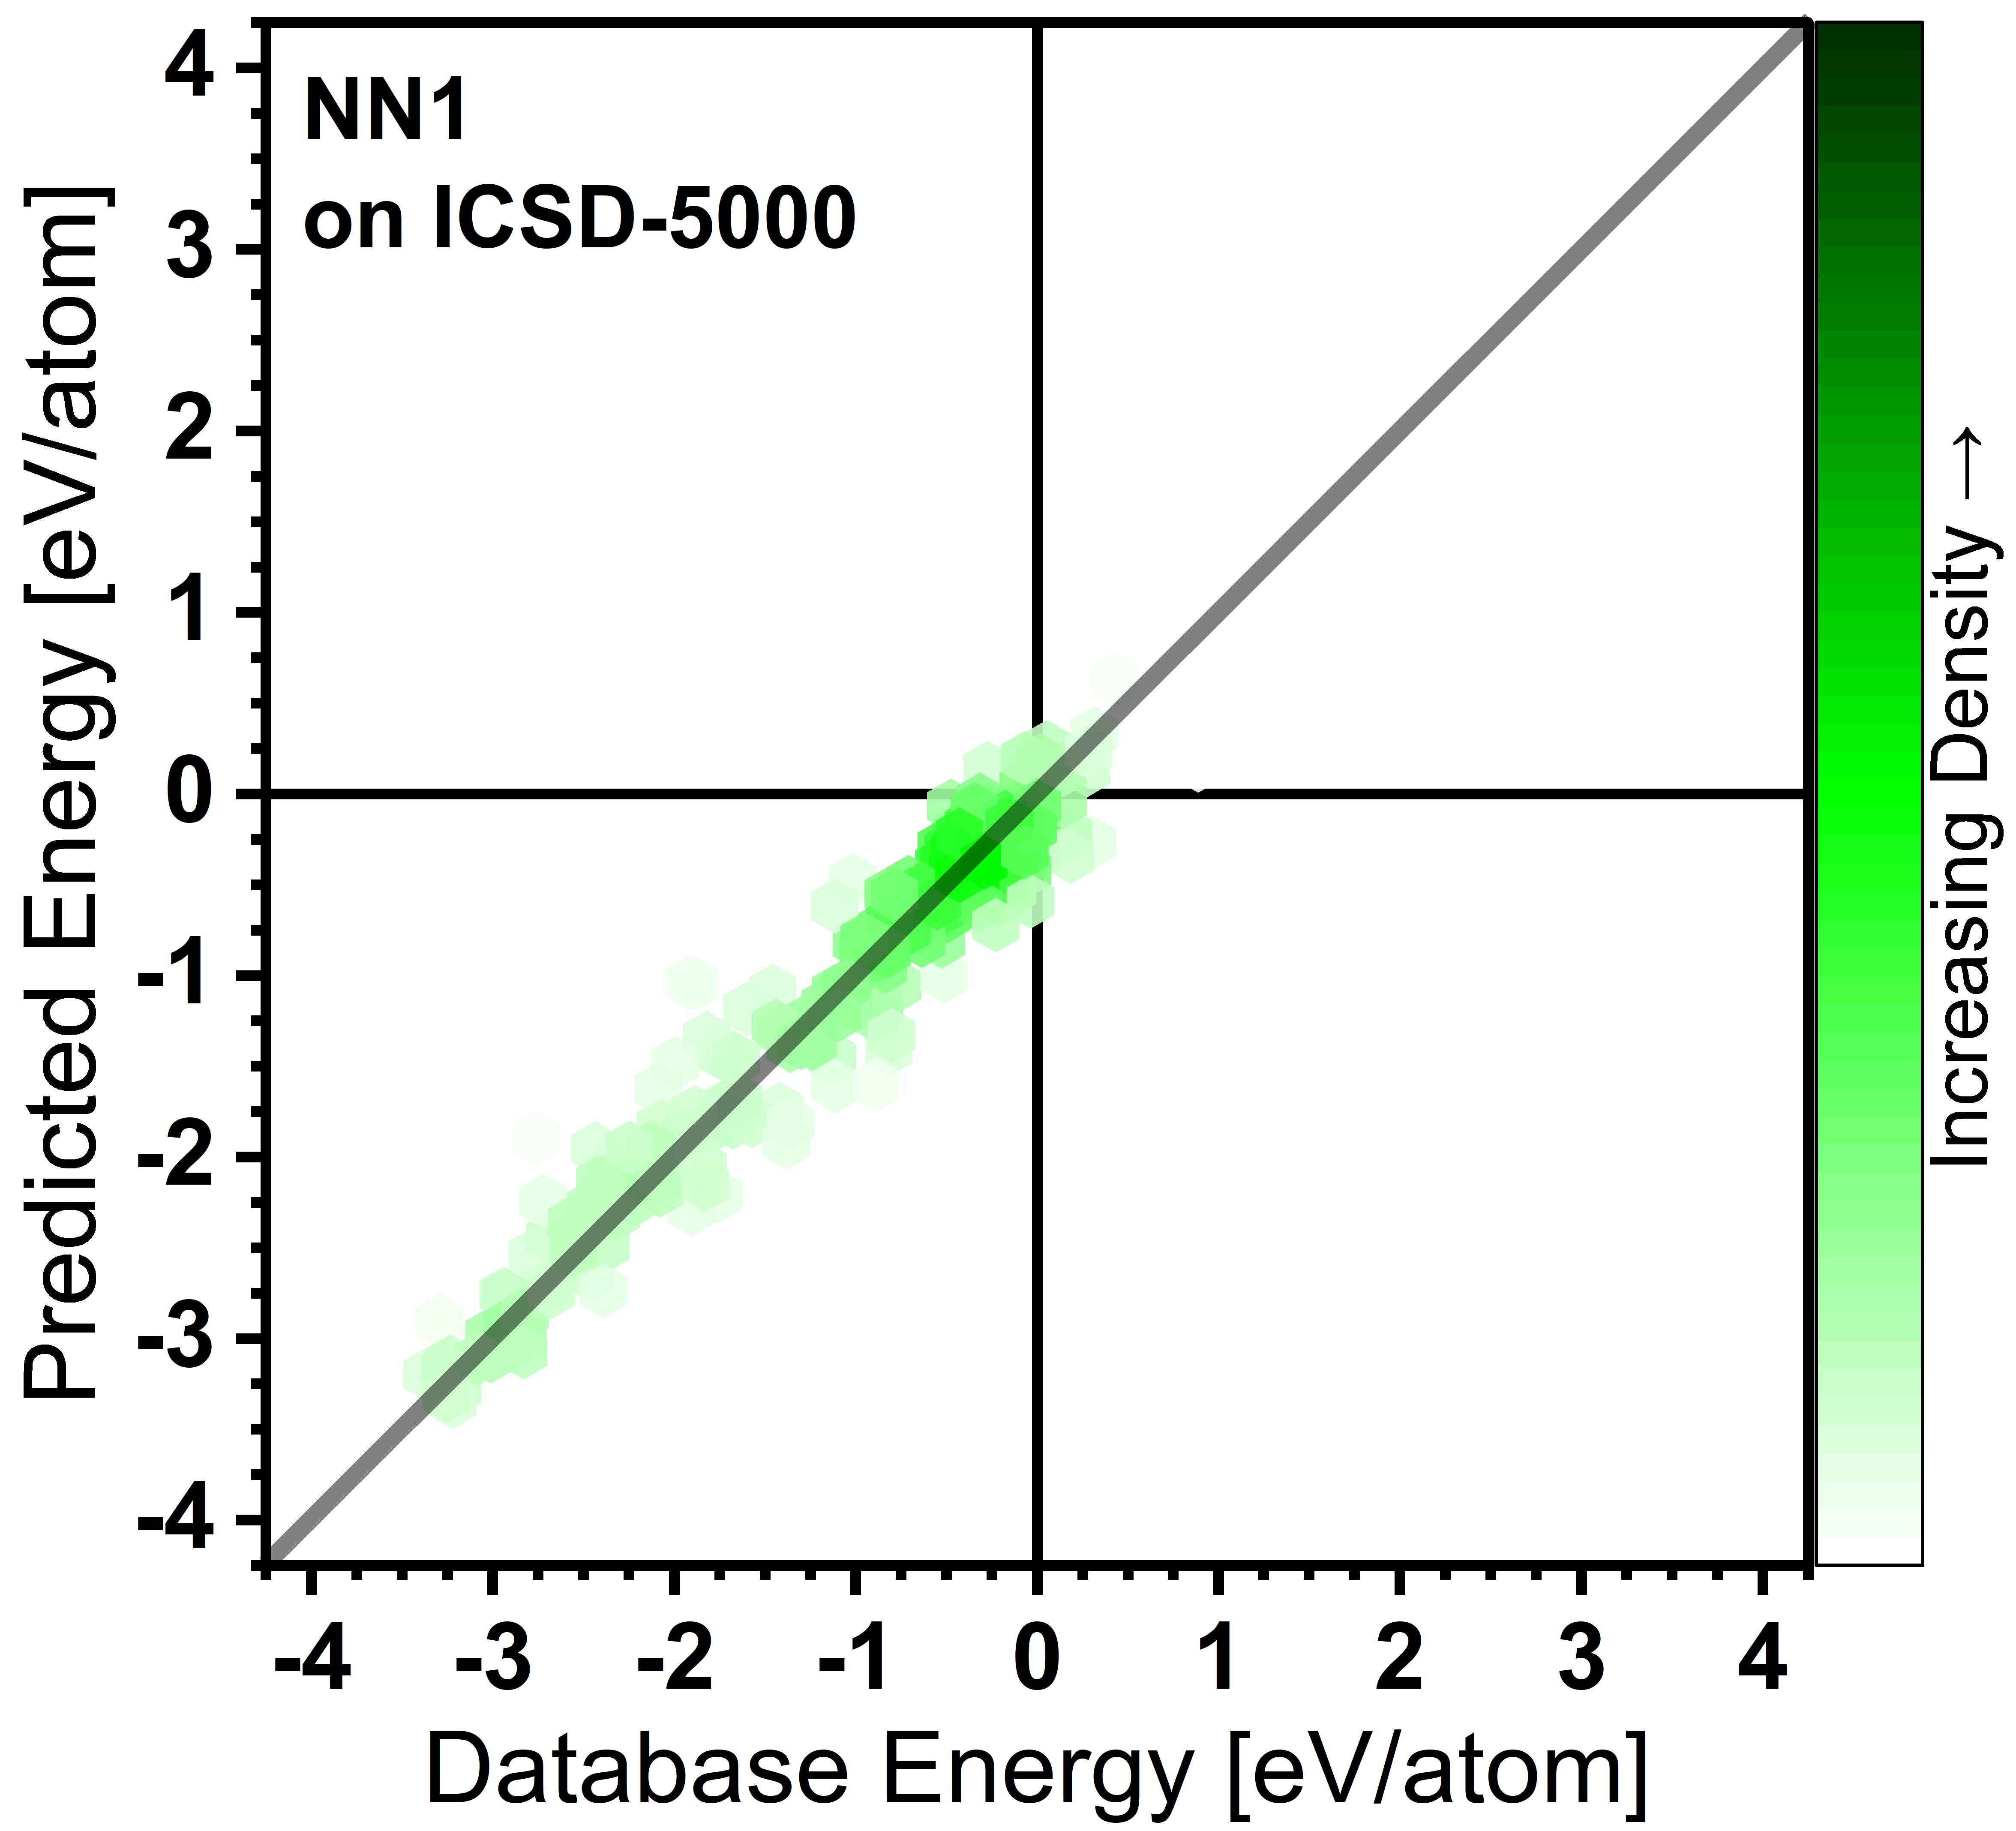
\includegraphics[width=0.35\textwidth]{sipfenn/NN1_test.png}
    \caption{Test of perceptron trained on the data from the first 5000 entries in the ICSD dataset and evaluated on the test set of 230 randomly selected entries ($\approx5\%$)}
    \label{sipfenn:fig:nn1performance}
\end{figure}

When trained on the data from all entries in the ICSD, it achieved an MAE of 364 meV/atom on the test set ($\approx5\% \text{ from } 32116$). This error is comparable to the performance of a random forest model based on PRDF (370 meV/atom), is slightly worse than a CM (250 meV/atom), and is significantly worse than a random-forest model trained on the same descriptor (90 meV/atom), as reported by Ward et al. \cite{Ward2017IncludingTessellations}. Part of the significance of these results is the evident quality of the descriptor, as the model achieved performance that would be considered excellent just a few years prior to the present work while being much less complex and computationally costly. Furthermore, it is important to note the time- and space-complexity of the perceptron model. Training the final network took less than 8 seconds compared to around 10,000 seconds reported for the aforementioned random-forest methods, and the resulting model occupied less than 1kb of memory. Following the testing of a perceptron, which allowed rough estimation of the a good size of the network (i.e. number of weights), the design of the actual architecture began. All of these steps are schematically depicted in Figure \ref{sipfenn:fig:designprocess}.

\begin{figure}[H]
    \centering
    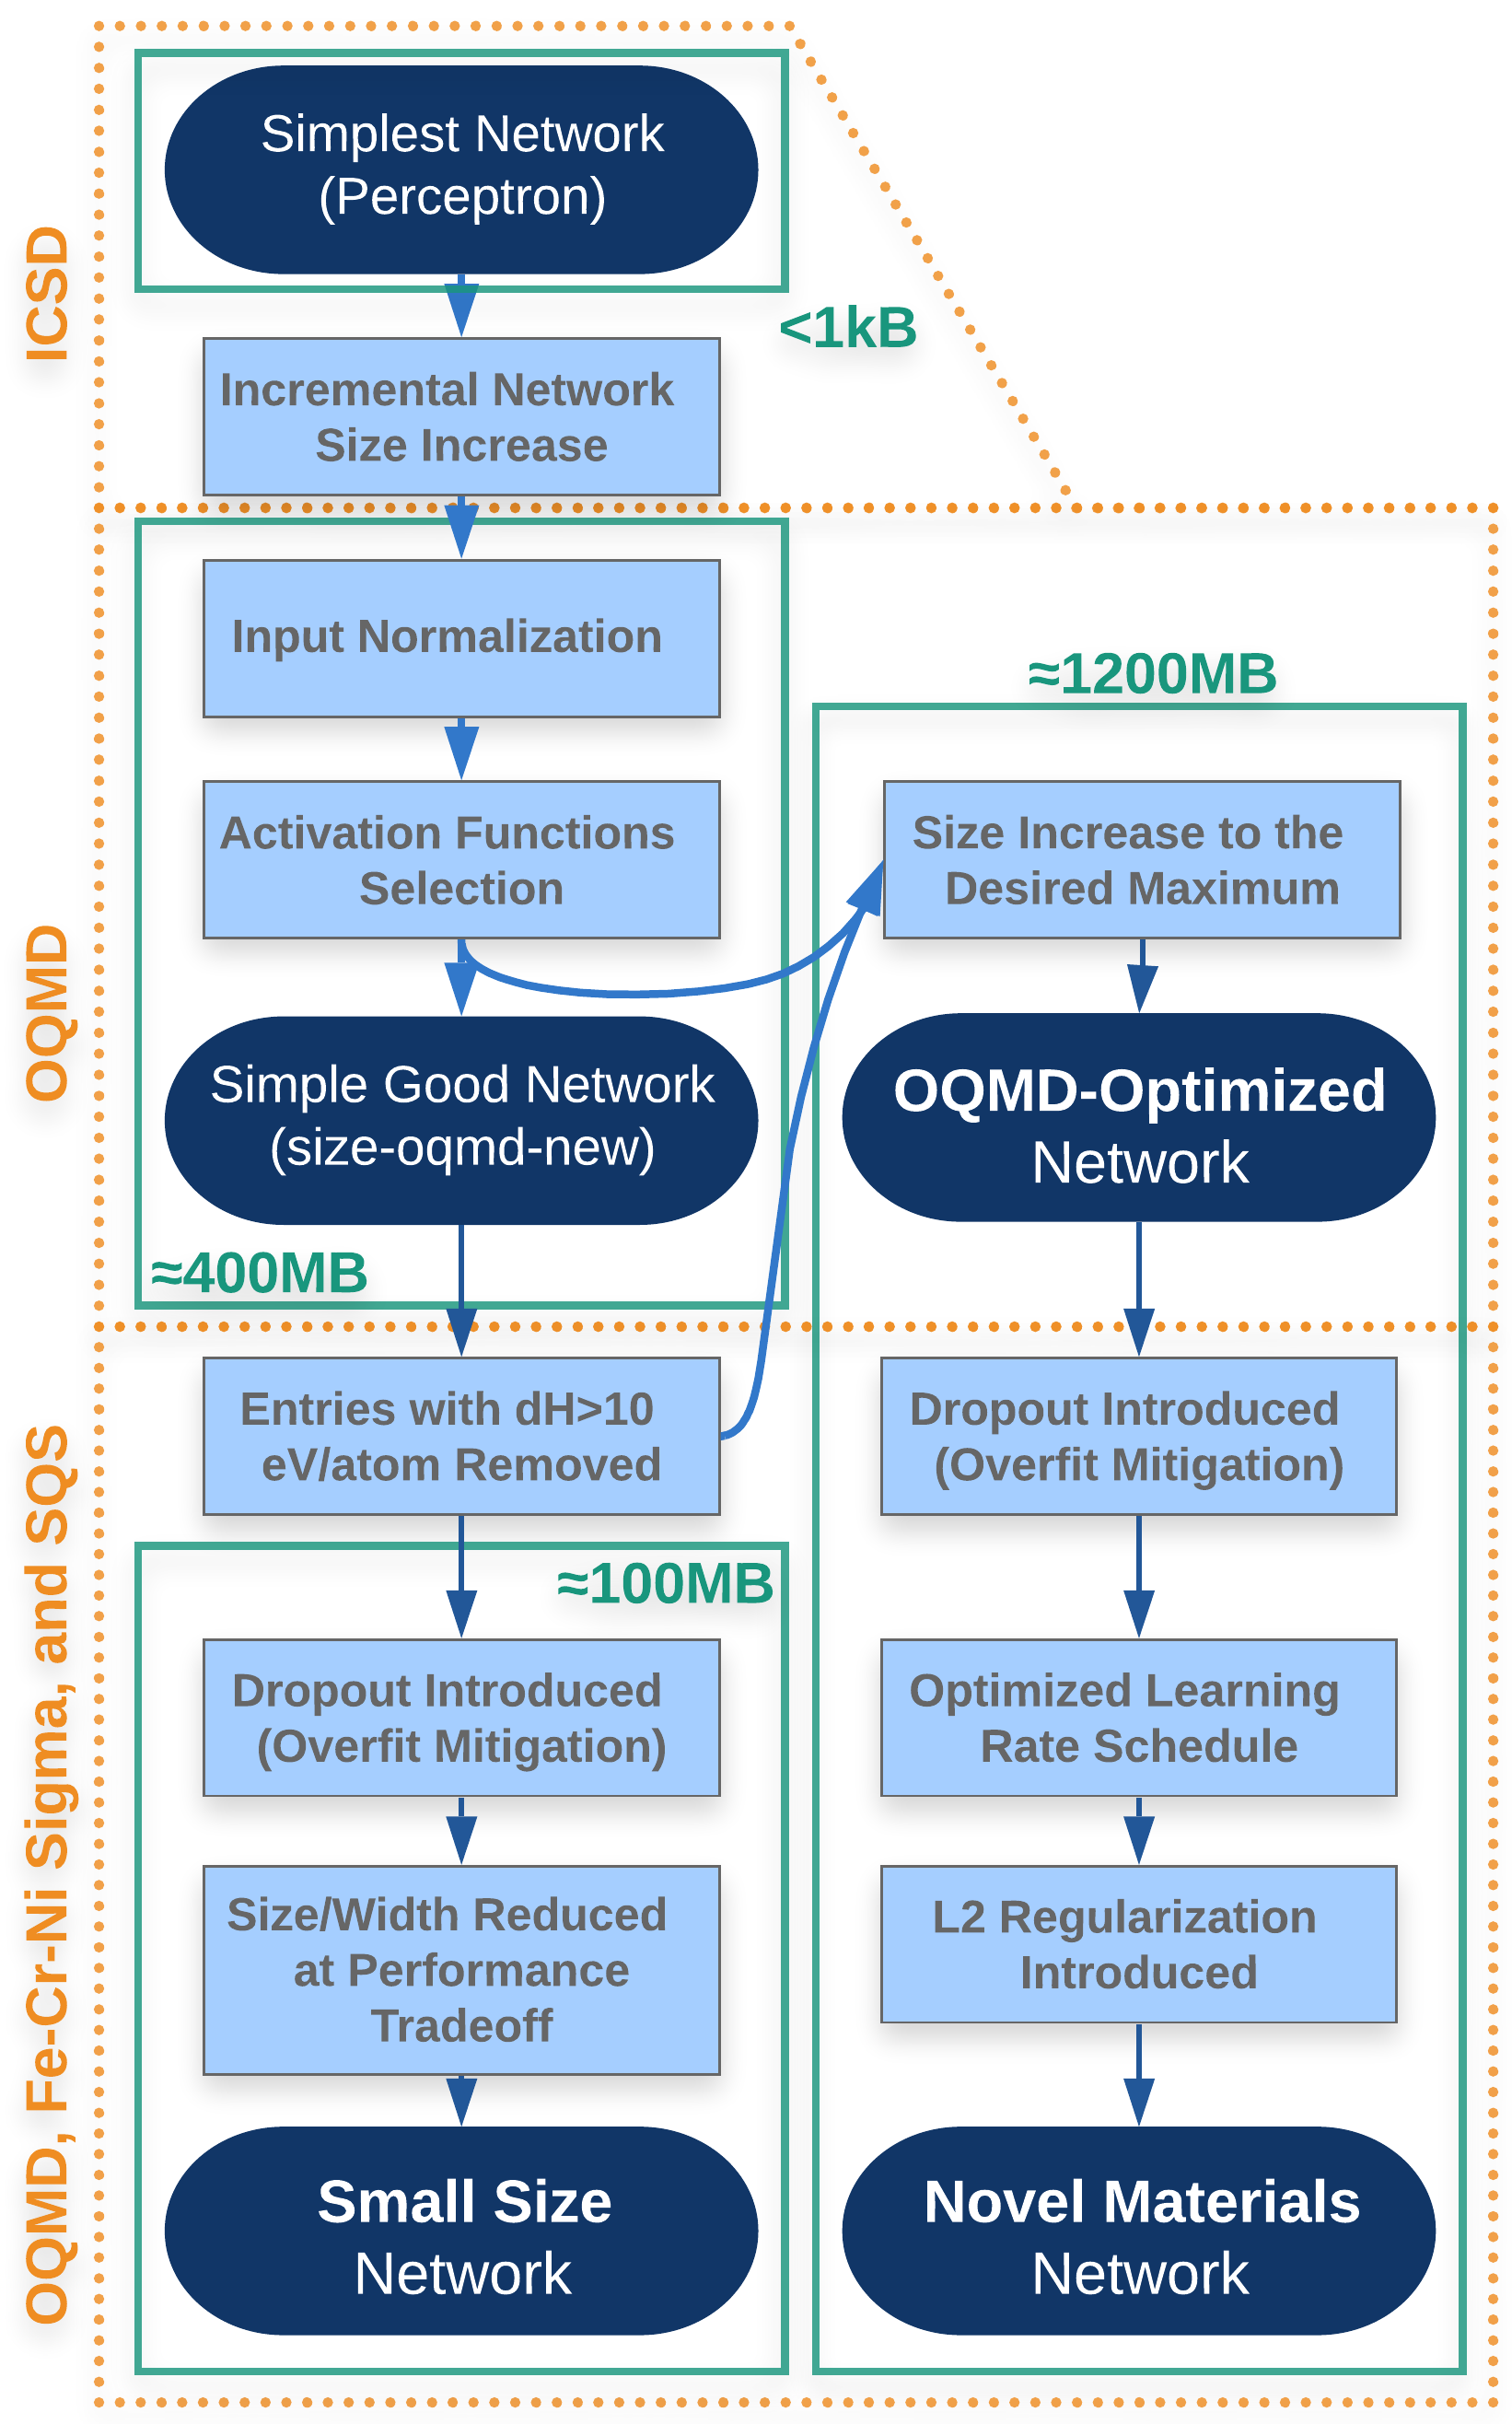
\includegraphics[width=0.5\textwidth]{sipfenn/SIPFENN_design_updated.png}
    \caption{The network design process schematic leading to the three final models. This figure is Figure \ref{sipfenn:fig:designprocess} cloned to the Appendix for conveninece.}
\end{figure}

Next, in a few steps, the size of the network was incrementally increased. First, a layer of 1000 neurons was introduced. This reduced the performance on the first 5000 entries in the ICSD, likely due to overfitting issues, as the data was very limited. Performance on the ICSD was improved, reducing the test MAE to 305 meV/atom on the test set, however. The introduction of the next two 1000-width layers further reduced the MAE to 215 meV/atom. Based on these results, it was estimated that introducing 4 hidden layers with Sigmoid activation function and widths of 10000, 10000, 1000, and 100 would provide good results when trained on the much larger OQMD.

After switching to OQMD, the network exhibited issues with convergence, often predicting a single value for all of the entries. To mitigate this, the descriptor (i.e. network input) was normalized by dividing every element by its maximum value across the whole dataset. This solved the issue. Next, to improve the training behavior, the activation functions were changed from only the Sigmoid function to a mix of Soft Sign, Exponential Linear Unit, and Sigmoid, which was found to work well. These steps improved both the predictive performance and reduced the time required to converge. The network architecture resulting from these steps (internally designated NN8 / Simple Good Network in Figure \ref{sipfenn:fig:designprocess}) was the first to improve performance compared to the Ward et. al approach \cite{Ward2017IncludingTessellations}, achieving an MAE of 42 meV/atom on the test set of random subset 5\% of the OQMD dataset. When testing this network, a small fraction of around 0.03\% of likely incorrect entries in the OQMD was found, as described in \ref{sipfenn:sssec:Data}, and was removed from the dataset used later in the design process.

Once a network with desired performance was obtained, the network size was increased until it either exceeded 1GB or showed signs of extensive overfitting. At the first step of this process, two layers of width 10,000 were added, resulting in a network size of 1.2GB and reduced overfitting, as indicated by the ratio of validation-to-training error lowered from 2.2 to 1.6, relative to NN8. The resulting network (internally designated NN9 / OQMD-Optimized Network in Figure \ref{sipfenn:fig:designprocess}), achieved an MAE of 28 meV/atom on the test set of random subset 5\% of OQMD, which was the best performance on OQMD out of all the networks created in this project. If the 0.03\% of abnormal data wasn't removed as described in \ref{sipfenn:sssec:Data}, it would correspond to, on average, 6 data points which in one tested instance increased the MAE to 35 meV/atom. Important to point out, the training of this network was prone to staying in local minima at the beginning. The reported instance of the trained network exhibited no training progress between around rounds 5 and 25, after which it's performance quickly increased.  Detailed analysis of the performance is given in \ref{sipfenn:ssec:oqmdperformance}.

Once the main objective of the design process was obtained, i.e. the performance on the OQMD has improved appreciably beyond existing methods, the design process was focused on creating a tool for modeling materials that were not reported in the OQMD. Therefore, the objective changed from achieving the lowest MAE on a random subset 5\% of OQMD to (1) reducing the mismatch between training and validation sets errors (i.e. difference between training accuracy and validation accuracy) during the training process, (2) keeping the test MAE on the OQMD below 50 meV/atom, and (3) improving performance on two material groups significantly different from the OQMD data, namely Special Quasirandom Structures (SQS) and Fe-Cr-Ni $\sigma$-phase (see \ref{sipfenn:sssec:Data}).

With these new objectives, two Dropout layers in the middle part of the network were introduced to promote the distribution of pattern recognition abilities across the network. \cite{Srivastava2014Dropout:Overfitting} This introduced a problem with convergence as the network became more likely to fall into local minima at the initial stages of the training, which was solved by introducing custom learning rate schedules. Specifically, the learning rate was initially set to a value orders of magnitude lower than during the default initial training and then ramped up to the previous (ADAM default setting in the majority of frameworks) learning rate of 0.001 (or above) after around 2 rounds of training. This type of learning rate schedule is known as a warm-up in the deep learning literature \cite{gotmare2018closer}. The schedule found to perform the best is presented in Figure \ref{sipfenn:fig:learningrate}.

\begin{figure}[H]
\centering
    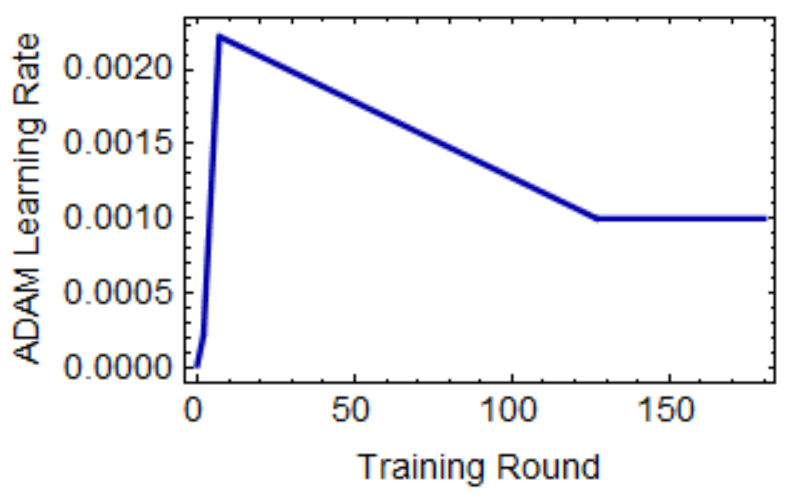
\includegraphics[width=0.35\textwidth]{sipfenn/nn18_learningrate_linonly.png}
    \caption{The learning rate schedule used for training of more complex networks in the later stage of the design process (e.g., NN18).}
    \label{sipfenn:fig:learningrate}
\end{figure}


The next step was the introduction of $\ell^2$ regularization, which is a technique that favors simplification of the descriptor and effectively rejects features of the descriptor that do not contribute to prediction performance \cite{L2Regularization}. An overview on it is given in Section \ref{sipfenn:ref:machinelearningoverview}. In the models reported in the present work an $\ell^2$ value of $10^{-6}$ was used. Higher values were found to stop the training at early stages, impairing the pattern recognition, or in extreme cases (above $10^{-3}$) force the network to discard the input completely, resulting in constant or near-constant output (i.e. mean value from the training dataset predicted for any structure).

The final step was small curation of the training data based on the OQMD-reported structure stability, i.e. the energy difference between the formation energy and the energy convex hull. The motivation for that was the notion that DFT results are inherently less accurate for unstable phases. In this step, all entries with energies of more than 2000 meV/atom above the convex hull were removed from the training set. Importantly, the validation and testing sets were not modified for consistent performance reporting.

All of these changes resulted in a neural network that has been optimized for predicting new materials. In the code and Supplementary materials, it is designated as NN20 (Novel Materials Network in Figure \ref{sipfenn:fig:designprocess}). Compared to the OQMD-optimized network it was derived from, the test MAE on the OQMD increased from 28 to 49 meV/atom. However, at the same time, the mismatch between the training and validation set was reduced from 1.57 to 1.38. Or, as presented earlier in Figure \ref{sipfenn:fig:trainingvalidation}, reduced to about 1.15 for the same training duration. Furthermore, a relatively large portion of this error can be attributed to some unstable structures that were removed from the training set, but not from the test set. Once entries with formation energies of more than 1000 meV/atom above the convex hull were removed, the test MAE decreased to only 38 meV/atom. Restricting the test set further to only somewhat stable structures (stability below 250 meV/atom) resulted in an MAE of 30 meV/atom.

While the new-material-optimized network presented an increased MAE across a random subset of the OQMD, performance has significantly improved on the Fe-Cr-Ni $\sigma-$phase described in \ref{sipfenn:sssec:Data}. The MAE has decreased from 55 to 41 meV/atom, indicating that the model based on this neural network is more capable of making predictions for new materials.

Once two performance-oriented models were developed, increasing the performance-to-cost ratio has been explored with the motivation that some studies would benefit from many times higher throughput at minor accuracy decrease. Architecture design started from the selection of a network with a balanced size-to-performance ratio (NN8) and the introduction of an overfitting mitigation technique (Dropout \cite{srivastava2014dropout}) used for the network optimized for new materials, as depicted in Figure \ref{sipfenn:sssec:NetDesign}. Next, the network was gradually narrowed (fewer neurons in layers) until the performance started to noticeably deteriorate (41.9 meV/atom for 5000- and 4000-width vs 42.1 for 3000-width). This approach allowed a significant reduction of the network size (and the computational intensity to run it) from around 1,200MB of the two other models to around 145MB. If an application demands even more of a reduction in model size and computational cost, the same procedure could be continued until some minimum required performance is retained. 


\section{Feature Ranking Learned During Formation Energy Modeling} 
\label{sipfenn:appendix3}

\begin{longtable}{|l|l|}
\caption{\texttt{SIPFENN}'s \texttt{NN20} Model Input Feature Ranking Learned During Formation Energy Modeling}
\label{sipfenn:appendix3:featureranking}\\
\hline
\multicolumn{1}{|c|}{\textbf{Descriptor Feature}} & \multicolumn{1}{c|}{\textbf{Normalized Squared Weights Sum}} \\ \hline
\endfirsthead
%
\endhead
%
mean\_NeighDiff\_shell1\_MeltingT & 1 \\ \hline
mean\_MeltingT & 0.97502 \\ \hline
max\_MeltingT & 0.73512 \\ \hline
mean\_NeighDiff\_shell1\_NdUnfilled & 0.69157 \\ \hline
MaxPackingEfficiency & 0.68889 \\ \hline
most\_MeltingT & 0.67373 \\ \hline
dev\_GSvolume\_pa & 0.61042 \\ \hline
var\_NeighDiff\_shell1\_Column & 0.58782 \\ \hline
var\_NeighDiff\_shell1\_CovalentRadius & 0.57826 \\ \hline
var\_NeighDiff\_shell1\_MeltingT & 0.57259 \\ \hline
maxdiff\_GSvolume\_pa & 0.55156 \\ \hline
dev\_MeltingT & 0.5286 \\ \hline
mean\_SpaceGroupNumber & 0.51761 \\ \hline
min\_MeltingT & 0.50437 \\ \hline
var\_CellVolume & 0.49467 \\ \hline
var\_NeighDiff\_shell1\_MendeleevNumber & 0.492 \\ \hline
min\_NeighDiff\_shell1\_MeltingT & 0.47853 \\ \hline
mean\_NeighDiff\_shell1\_Column & 0.45566 \\ \hline
maxdiff\_CovalentRadius & 0.42998 \\ \hline
var\_NeighDiff\_shell1\_Electronegativity & 0.42642 \\ \hline
var\_EffectiveCoordination & 0.40506 \\ \hline
min\_NeighDiff\_shell1\_Column & 0.39822 \\ \hline
dev\_NdUnfilled & 0.39739 \\ \hline
dev\_CovalentRadius & 0.36935 \\ \hline
range\_NeighDiff\_shell1\_Column & 0.35956 \\ \hline
range\_NeighDiff\_shell1\_CovalentRadius & 0.34585 \\ \hline
mean\_WCMagnitude\_Shell1 & 0.34275 \\ \hline
mean\_NeighDiff\_shell1\_MendeleevNumber & 0.33911 \\ \hline
mean\_EffectiveCoordination & 0.33899 \\ \hline
mean\_Number & 0.33769 \\ \hline
mean\_NdUnfilled & 0.33408 \\ \hline
maxdiff\_MeltingT & 0.33348 \\ \hline
mean\_AtomicWeight & 0.33149 \\ \hline
mean\_NeighDiff\_shell1\_NdValence & 0.33142 \\ \hline
range\_NeighDiff\_shell1\_MeltingT & 0.33107 \\ \hline
max\_NfUnfilled & 0.33041 \\ \hline
dev\_Electronegativity & 0.33001 \\ \hline
mean\_NeighDiff\_shell1\_CovalentRadius & 0.32999 \\ \hline
var\_NeighDiff\_shell1\_NdUnfilled & 0.31973 \\ \hline
dev\_Column & 0.31662 \\ \hline
var\_NeighDiff\_shell1\_NdValence & 0.31481 \\ \hline
mean\_WCMagnitude\_Shell2 & 0.31359 \\ \hline
most\_NfUnfilled & 0.30916 \\ \hline
MeanIonicChar & 0.30732 \\ \hline
mean\_NeighDiff\_shell1\_Electronegativity & 0.30277 \\ \hline
min\_EffectiveCoordination & 0.29705 \\ \hline
min\_NeighDiff\_shell1\_CovalentRadius & 0.29392 \\ \hline
max\_NeighDiff\_shell1\_GSvolume\_pa & 0.2875 \\ \hline
most\_SpaceGroupNumber & 0.28472 \\ \hline
max\_NdUnfilled & 0.28424 \\ \hline
maxdiff\_NdUnfilled & 0.28405 \\ \hline
var\_NeighDiff\_shell1\_GSvolume\_pa & 0.28008 \\ \hline
min\_BondLengthVariation & 0.27922 \\ \hline
var\_MeanBondLength & 0.2768 \\ \hline
dev\_NdValence & 0.27566 \\ \hline
max\_NeighDiff\_shell1\_MeltingT & 0.27097 \\ \hline
max\_BondLengthVariation & 0.26565 \\ \hline
mean\_NfValence & 0.26558 \\ \hline
mean\_NsUnfilled & 0.2612 \\ \hline
max\_NeighDiff\_shell1\_CovalentRadius & 0.26026 \\ \hline
max\_GSvolume\_pa & 0.25985 \\ \hline
min\_GSvolume\_pa & 0.25895 \\ \hline
mean\_NdValence & 0.25573 \\ \hline
mean\_NeighDiff\_shell1\_GSvolume\_pa & 0.25299 \\ \hline
max\_NValance & 0.24749 \\ \hline
range\_NeighDiff\_shell1\_NdUnfilled & 0.24643 \\ \hline
max\_CovalentRadius & 0.23136 \\ \hline
CanFormIonic & 0.23135 \\ \hline
min\_NeighDiff\_shell1\_Electronegativity & 0.22873 \\ \hline
min\_SpaceGroupNumber & 0.22766 \\ \hline
max\_Electronegativity & 0.22609 \\ \hline
max\_NdValence & 0.22576 \\ \hline
most\_NdUnfilled & 0.22198 \\ \hline
min\_NeighDiff\_shell1\_MendeleevNumber & 0.21991 \\ \hline
var\_NeighDiff\_shell1\_NpValence & 0.21609 \\ \hline
min\_NeighDiff\_shell1\_NdUnfilled & 0.2114 \\ \hline
dev\_SpaceGroupNumber & 0.2099 \\ \hline
most\_NfValence & 0.20888 \\ \hline
min\_MeanBondLength & 0.2086 \\ \hline
mean\_BondLengthVariation & 0.20507 \\ \hline
var\_NeighDiff\_shell1\_Row & 0.20454 \\ \hline
max\_NeighDiff\_shell1\_NdUnfilled & 0.20318 \\ \hline
min\_NeighDiff\_shell1\_NdValence & 0.20123 \\ \hline
min\_CovalentRadius & 0.19974 \\ \hline
range\_NeighDiff\_shell1\_MendeleevNumber & 0.19591 \\ \hline
min\_NeighDiff\_shell1\_GSvolume\_pa & 0.19565 \\ \hline
most\_NpUnfilled & 0.19457 \\ \hline
maxdiff\_NUnfilled & 0.19316 \\ \hline
max\_NeighDiff\_shell1\_NdValence & 0.19307 \\ \hline
max\_NpValence & 0.1929 \\ \hline
range\_NeighDiff\_shell1\_GSvolume\_pa & 0.19166 \\ \hline
most\_NdValence & 0.1904 \\ \hline
max\_MeanBondLength & 0.19021 \\ \hline
maxdiff\_NfUnfilled & 0.18897 \\ \hline
max\_NeighDiff\_shell1\_Column & 0.18518 \\ \hline
range\_NeighDiff\_shell1\_Electronegativity & 0.18322 \\ \hline
var\_NeighDiff\_shell1\_SpaceGroupNumber & 0.18313 \\ \hline
dev\_NpValence & 0.18099 \\ \hline
mean\_NpUnfilled & 0.18091 \\ \hline
range\_NeighDiff\_shell1\_SpaceGroupNumber & 0.17858 \\ \hline
dev\_MendeleevNumber & 0.17753 \\ \hline
MaxIonicChar & 0.176 \\ \hline
mean\_Column & 0.17206 \\ \hline
min\_Electronegativity & 0.17164 \\ \hline
mean\_WCMagnitude\_Shell3 & 0.17077 \\ \hline
mean\_Row & 0.17035 \\ \hline
min\_NeighDiff\_shell1\_SpaceGroupNumber & 0.17031 \\ \hline
most\_NsUnfilled & 0.16714 \\ \hline
var\_BondLengthVariation & 0.16653 \\ \hline
var\_NeighDiff\_shell1\_NfUnfilled & 0.16223 \\ \hline
range\_NeighDiff\_shell1\_NdValence & 0.16094 \\ \hline
frac\_fValence & 0.1609 \\ \hline
maxdiff\_Column & 0.16083 \\ \hline
max\_NUnfilled & 0.15916 \\ \hline
mean\_NpValence & 0.15639 \\ \hline
maxdiff\_NpValence & 0.15637 \\ \hline
mean\_MendeleevNumber & 0.15491 \\ \hline
most\_Electronegativity & 0.15469 \\ \hline
mean\_Electronegativity & 0.15458 \\ \hline
max\_SpaceGroupNumber & 0.15429 \\ \hline
dev\_Row & 0.15382 \\ \hline
maxdiff\_MendeleevNumber & 0.15373 \\ \hline
var\_NeighDiff\_shell1\_NpUnfilled & 0.15135 \\ \hline
max\_NeighDiff\_shell1\_Electronegativity & 0.15115 \\ \hline
most\_NUnfilled & 0.14955 \\ \hline
max\_GSbandgap & 0.14945 \\ \hline
mean\_NeighDiff\_shell1\_NUnfilled & 0.14891 \\ \hline
maxdiff\_NValance & 0.14819 \\ \hline
mean\_NeighDiff\_shell1\_NpValence & 0.14768 \\ \hline
maxdiff\_NdValence & 0.14735 \\ \hline
max\_NpUnfilled & 0.14647 \\ \hline
maxdiff\_Electronegativity & 0.14523 \\ \hline
min\_MendeleevNumber & 0.14119 \\ \hline
mean\_CovalentRadius & 0.14049 \\ \hline
mean\_NeighDiff\_shell1\_Row & 0.13945 \\ \hline
maxdiff\_GSbandgap & 0.13891 \\ \hline
max\_NeighDiff\_shell1\_MendeleevNumber & 0.13858 \\ \hline
most\_Number & 0.13823 \\ \hline
most\_AtomicWeight & 0.13798 \\ \hline
max\_NeighDiff\_shell1\_NpValence & 0.13757 \\ \hline
Comp\_L10Norm & 0.13598 \\ \hline
min\_Row & 0.13596 \\ \hline
range\_NeighDiff\_shell1\_NpValence & 0.13524 \\ \hline
mean\_GSvolume\_pa & 0.1331 \\ \hline
max\_NeighDiff\_shell1\_NUnfilled & 0.13205 \\ \hline
mean\_NeighDiff\_shell1\_NfValence & 0.12888 \\ \hline
min\_NeighDiff\_shell1\_NpUnfilled & 0.12778 \\ \hline
mean\_NeighDiff\_shell1\_SpaceGroupNumber & 0.12722 \\ \hline
mean\_NsValence & 0.12642 \\ \hline
most\_CovalentRadius & 0.12616 \\ \hline
var\_NeighDiff\_shell1\_NUnfilled & 0.12525 \\ \hline
mean\_NeighDiff\_shell1\_Number & 0.12466 \\ \hline
Comp\_L7Norm & 0.12293 \\ \hline
mean\_NeighDiff\_shell1\_AtomicWeight & 0.12229 \\ \hline
min\_NeighDiff\_shell1\_NpValence & 0.12026 \\ \hline
max\_EffectiveCoordination & 0.11995 \\ \hline
min\_NdValence & 0.11984 \\ \hline
maxdiff\_NpUnfilled & 0.11976 \\ \hline
mean\_NeighDiff\_shell1\_NsUnfilled & 0.11836 \\ \hline
max\_NeighDiff\_shell1\_GSbandgap & 0.11657 \\ \hline
min\_NUnfilled & 0.11648 \\ \hline
most\_Column & 0.1164 \\ \hline
var\_NeighDiff\_shell1\_Number & 0.11483 \\ \hline
most\_MendeleevNumber & 0.11312 \\ \hline
max\_NeighDiff\_shell1\_SpaceGroupNumber & 0.11292 \\ \hline
var\_NeighDiff\_shell1\_AtomicWeight & 0.11234 \\ \hline
most\_NpValence & 0.11231 \\ \hline
frac\_dValence & 0.11126 \\ \hline
NComp & 0.11097 \\ \hline
min\_Number & 0.11062 \\ \hline
range\_NeighDiff\_shell1\_NpUnfilled & 0.11002 \\ \hline
dev\_NValance & 0.10868 \\ \hline
min\_Column & 0.10846 \\ \hline
max\_NeighDiff\_shell1\_NpUnfilled & 0.10837 \\ \hline
maxdiff\_Row & 0.10735 \\ \hline
Comp\_L5Norm & 0.10726 \\ \hline
mean\_NeighDiff\_shell1\_NpUnfilled & 0.10682 \\ \hline
maxdiff\_SpaceGroupNumber & 0.10604 \\ \hline
dev\_GSbandgap & 0.10604 \\ \hline
max\_AtomicWeight & 0.10495 \\ \hline
max\_GSmagmom & 0.10416 \\ \hline
maxdiff\_GSmagmom & 0.1039 \\ \hline
dev\_NUnfilled & 0.10336 \\ \hline
var\_NeighDiff\_shell1\_NfValence & 0.10059 \\ \hline
dev\_GSmagmom & 0.10046 \\ \hline
most\_GSbandgap & 0.09997 \\ \hline
var\_NeighDiff\_shell1\_NValance & 0.09842 \\ \hline
min\_NeighDiff\_shell1\_Row & 0.09798 \\ \hline
min\_NeighDiff\_shell1\_NUnfilled & 0.09563 \\ \hline
most\_Row & 0.09538 \\ \hline
max\_Number & 0.0925 \\ \hline
most\_GSvolume\_pa & 0.09166 \\ \hline
mean\_GSbandgap & 0.09097 \\ \hline
range\_NeighDiff\_shell1\_Row & 0.09081 \\ \hline
mean\_NValance & 0.0889 \\ \hline
mean\_NeighDiff\_shell1\_NsValence & 0.08449 \\ \hline
min\_NsValence & 0.08408 \\ \hline
frac\_pValence & 0.08403 \\ \hline
mean\_NUnfilled & 0.08244 \\ \hline
mean\_NfUnfilled & 0.08194 \\ \hline
dev\_NpUnfilled & 0.0818 \\ \hline
dev\_Number & 0.08065 \\ \hline
max\_NeighDiff\_shell1\_GSmagmom & 0.08049 \\ \hline
max\_Column & 0.07989 \\ \hline
min\_AtomicWeight & 0.07959 \\ \hline
Comp\_L3Norm & 0.07913 \\ \hline
max\_NeighDiff\_shell1\_Row & 0.0776 \\ \hline
mean\_NeighDiff\_shell1\_NValance & 0.07619 \\ \hline
mean\_NeighDiff\_shell1\_NfUnfilled & 0.07413 \\ \hline
range\_NeighDiff\_shell1\_NfUnfilled & 0.07381 \\ \hline
min\_NValance & 0.07297 \\ \hline
max\_NeighDiff\_shell1\_NValance & 0.0726 \\ \hline
range\_NeighDiff\_shell1\_NfValence & 0.07163 \\ \hline
min\_NdUnfilled & 0.07145 \\ \hline
most\_NsValence & 0.07114 \\ \hline
mean\_NeighDiff\_shell1\_GSbandgap & 0.06709 \\ \hline
max\_NfValence & 0.06661 \\ \hline
dev\_AtomicWeight & 0.06581 \\ \hline
maxdiff\_Number & 0.06576 \\ \hline
max\_NeighDiff\_shell1\_NfUnfilled & 0.06523 \\ \hline
dev\_NfUnfilled & 0.06477 \\ \hline
dev\_NfValence & 0.06373 \\ \hline
range\_NeighDiff\_shell1\_GSmagmom & 0.06305 \\ \hline
var\_NeighDiff\_shell1\_NsUnfilled & 0.06288 \\ \hline
min\_NeighDiff\_shell1\_Number & 0.0623 \\ \hline
frac\_sValence & 0.06099 \\ \hline
min\_NeighDiff\_shell1\_NfValence & 0.06033 \\ \hline
max\_Row & 0.05998 \\ \hline
min\_NeighDiff\_shell1\_NValance & 0.05844 \\ \hline
range\_NeighDiff\_shell1\_NUnfilled & 0.05819 \\ \hline
var\_NeighDiff\_shell1\_GSbandgap & 0.05683 \\ \hline
range\_NeighDiff\_shell1\_AtomicWeight & 0.0568 \\ \hline
Comp\_L2Norm & 0.05638 \\ \hline
min\_NeighDiff\_shell1\_NsUnfilled & 0.05541 \\ \hline
most\_NValance & 0.0553 \\ \hline
maxdiff\_NsValence & 0.05459 \\ \hline
range\_NeighDiff\_shell1\_NValance & 0.0537 \\ \hline
min\_NeighDiff\_shell1\_AtomicWeight & 0.05369 \\ \hline
max\_NsValence & 0.05329 \\ \hline
range\_NeighDiff\_shell1\_GSbandgap & 0.05299 \\ \hline
min\_NeighDiff\_shell1\_NfUnfilled & 0.05266 \\ \hline
maxdiff\_NfValence & 0.05147 \\ \hline
dev\_NsUnfilled & 0.04884 \\ \hline
max\_MendeleevNumber & 0.04844 \\ \hline
maxdiff\_AtomicWeight & 0.04814 \\ \hline
max\_NeighDiff\_shell1\_NsUnfilled & 0.04675 \\ \hline
max\_NeighDiff\_shell1\_NsValence & 0.04663 \\ \hline
var\_NeighDiff\_shell1\_GSmagmom & 0.04635 \\ \hline
range\_NeighDiff\_shell1\_Number & 0.04416 \\ \hline
max\_NeighDiff\_shell1\_NfValence & 0.04376 \\ \hline
mean\_NeighDiff\_shell1\_GSmagmom & 0.0433 \\ \hline
most\_GSmagmom & 0.04239 \\ \hline
range\_NeighDiff\_shell1\_NsUnfilled & 0.03954 \\ \hline
min\_NeighDiff\_shell1\_NsValence & 0.03932 \\ \hline
max\_NeighDiff\_shell1\_AtomicWeight & 0.03905 \\ \hline
max\_NeighDiff\_shell1\_Number & 0.03815 \\ \hline
min\_NfValence & 0.03794 \\ \hline
dev\_NsValence & 0.0373 \\ \hline
maxdiff\_NsUnfilled & 0.03558 \\ \hline
min\_NfUnfilled & 0.03537 \\ \hline
min\_NeighDiff\_shell1\_GSmagmom & 0.03353 \\ \hline
var\_NeighDiff\_shell1\_NsValence & 0.02948 \\ \hline
min\_NpValence & 0.02946 \\ \hline
max\_NsUnfilled & 0.02933 \\ \hline
min\_NeighDiff\_shell1\_GSbandgap & 0.02735 \\ \hline
mean\_GSmagmom & 0.02402 \\ \hline
min\_NpUnfilled & 0.02233 \\ \hline
range\_NeighDiff\_shell1\_NsValence & 0.02171 \\ \hline
min\_NsUnfilled & 0.02051 \\ \hline
min\_GSbandgap & 0.01299 \\ \hline
min\_GSmagmom & 0.00132 \\ \hline
\end{longtable}

\section{Extended Statistics and Visualizations of Materials-Property-Descriptor Database} \label{mpdd:app1}

The three key statistics presented in Figure~\ref{mpdd:fig:dataset} are a small subset of the larger dashboard available at \href{https://phaseslab.org/mpdd}{phaseslab.org/mpdd} web page, which is presented in Figure~\ref{sup:mpdd:dashboard}.

\begin{figure}[H]
    \centering
    \includegraphics[width=0.95\textwidth]{mpdd/mpdddashboard.png}
    \caption{The main MPDD dashboard with statistics over MPDD dataset, as of April 2024, demonstrating the dataset in terms of different levels of "corese-graining" the uniqueness criteria, and coverage of chemical systems of different order.}
    \label{sup:mpdd:dashboard}
\end{figure}

Partial data on all of the MPDD data points can be accessed through a graphical user interface (GUI), available at \href{https://mpdd.org}{mpdd.org}, presented in Figure~\ref{sup:mpdd:gui}. It enables users to query the database based on fields including chemical formula, chemical system, or space group number, to facilitate easy access for users not familiar with programming and those who only need to access a small subset of it.

\begin{figure}[H]
    \centering
    \includegraphics[width=0.95\textwidth]{mpdd/mpddgui.png}
    \caption{A basic MPDD graphical user interface (GUI) set up for easy access to the data based on a couple of common query fields.}
    \label{sup:mpdd:gui}
\end{figure}

The OPTIMADE API \cite{Evans2024DevelopmentsExchange}, as discussed in Section~\ref{mpdd:sec:optimade}, can be accessed using software like \texttt{optimade-python-tools} \cite{Evans2021} or by going to the \href{http://optimade.mpdd.org}{optimade.mpdd.org} endpoint. Figure~\ref{sup:mpdd:optimade} depicts the expected web page, as of May 2024.

\begin{figure}[H]
    \centering
    \includegraphics[width=0.9\textwidth]{mpdd/mpddoptimade.png}
    \caption{Printout of the MPDD OPTIMADE API endpoint page.}
    \label{sup:mpdd:optimade}
\end{figure}

One can use the endpoint page shown in Figure~\ref{sup:mpdd:optimade} to quickly check (1) accessibility of the database, and (2) investigate its schema, by following endpoint like \href{http://optimade.mpdd.org/v1/structures}{optimade.mpdd.org/v1/structures} to see example data response, like the one shown in Figure~\ref{sup:mpdd:optimadeout}, or \href{http://optimade.mpdd.org/v1/info}{optimade.mpdd.org/v1/info} to see MPDD provider information page.

\begin{figure}[H]
    \centering
    \includegraphics[width=0.95\textwidth]{mpdd/mpddoptimadeout.png}
    \caption{An example printout of (partial) MPDD's OPTIMADE response upon a query to the \texttt{http://optimade.mpdd.org/v1/structures} endpoint, depicting human-unreadable but machine-readable output.}
    \label{sup:mpdd:optimadeout}
\end{figure}


\section{Motivation for Multi-Grade Compositional Design of Materials Exemplified with Hf-Zr Powders} \label{nimplex:app1}

As mentioned in Section~\ref{nimplex:ssec:functionallygraded}, different grades of base metals may have very different costs associated with them. For instance, as of December 2023, at \href{https://www.fishersci.com}{Fisher Scientific online store (fishersci.com)}, one can purchase:
\begin{itemize}
    \item High-purity Zr wire: $250cm$ of $0.25mm$-diameter (AA00416CB) for $\$317$ or $\approx 390\frac{\$}{g}$
    \item $99.2\%$ (Zr+$4.5\%$Hf) wire: $200cm$ of $0.25mm$-diameter (AA43334G2) for $\$63$ or $\approx 100\frac{\$}{g}$. 
    \item $99.97\%$ (Hf+$3\%$Zr) wire: $200cm$ of $0.25mm$-diameter (AA10200G2) for $\$200$ or $\approx 156\frac{\$}{g}$. 
\end{itemize} 

Now, if one tries to create FGMs which navigates Zr-rich regions in Hf-containing space, there are two possible choices for Zr source, namely, pure Zr or the (Zr+$4.5\%Hf$) alloy. The first one enables all possible Zr fractions, unlike the latter which establishes the minimum Hf fraction at 4.5\% at the "Zr" corner of the attainable space tetrahedron (anonymous example of this is in Figure~\ref{nimplex:fig:fgmspaces}). Such an ability may be necessary, e.g., to avoid infeasible regions of space, but if not, it represents an unnecessary cost. 

For instance, to obtain (Zr+$10\%wt$Hf) alloy, one can combine high-purity Zr and (Hf+$3\%Zr$) for $\approx 360\frac{\$}{g}$ or equivalently from (Zr+$4.5\%$Hf) and (Hf+$3\%$Zr) for $\approx 103\frac{\$}{g}$, representing 3.5 times cost reduction.

At Fisher Scientific, as of writing this, the pure-Zr wire is only available in $0.25mm$ diameter, thus, the above considerations were restricted to it to keep the comparisons fair. However, for the (Zr+$4.5\%$Hf) grade, many less-expensive form factors are available as it is much more industry relevant. Furthermore, larger package sizes ($\geq50g$) are available driving the cost down further. For instance, the following $1mm$ wires can be purchased:

\begin{itemize}
    \item $99.2\%$ (Zr+$4.5\%$Hf) wire: $10m$ of $1mm$-diameter  (AA14627H2) for $\$130$ or $\approx 2.5\frac{\$}{g}$. 
    \item $99.97\%$ (Hf+$3\%$Zr) wire: $5m$ of $1mm$-diameter (AA10205CC) for $\$580$ or $\approx 11.3\frac{\$}{g}$. 
\end{itemize}

If the above are used, one can now obtain the same (Zr+$10\%wt$Hf) alloy for $\approx 3\frac{\$}{g}$ or 120 times cheaper relative to using high purity Zr in the only available physical form factor.
    

\section{Geometric Cross-Evidence for Factorial Decay of Simplex Space in Equally Dimensional Cartesian Space}  \label{nimplex:app2}

The equation for the fraction of a cube bound by [111] plane, equivalent to the result for $f(4)$ in Section~\ref{nimplex:sec:randomuniformsampling}, can be quickly obtained by considering that the volume of a pyramid is given by $V = \frac{A_B h}{3}$, where $A_B$ is the base area of equilateral triangle $\frac{\sqrt{3}}{4}\times\sqrt{2}^2 = \frac{\sqrt{3}}{2}$ and $h$ is $\frac{1}{\sqrt{3}}$. Thus we get 
$$V = \frac{\frac{\sqrt{3}}{2} \frac{1}{\sqrt{3}}}{3} = \frac{1}{6}$$ 
agreeing with the aforementioned result in Section~\ref{nimplex:sec:randomuniformsampling}.


\section{Bidirectional \texttt{neighborsLink4C} Algorithm found Conceptually}  \label{nimplex:app3}

The equation for "forward" and "backward" jumps in 3-simplex graph corresponding to a quaternary chemical system. 

\begin{minted}[xleftmargin=3\parindent, fontsize=\small]{nim}
proc neighborsLink4C(
    i:int, x:Tensor, neighbors: var seq[seq[int]], ndiv: int): void =
  let jump0 = 1  #binom(x, 0)=1
  let jump1 = binom(1+ndiv-x[0]-x[1], 1)
  let jump2 = binom(2+ndiv-x[0], 2)
  
  if x[0] != 0:
    # quaternary
    neighbors[i].add(i - jump2)
    # quaternary
    neighbors[i].add(i - jump2 - jump1)
    # quaternary
    neighbors[i].add(i - jump2 - jump1 - jump0) 
  
  if x[1] != 0:
    # ternary
    neighbors[i].add(i - jump1)    
    # ternary
    neighbors[i].add(i - jump1 - jump0)         
    # quaternary
    neighbors[i].add(i + jump2 - jump1 - x[1])  
  
  if x[2] != 0:
    # binary
    neighbors[i].add(i - jump0)     
    # ternary
    neighbors[i].add(i + jump1 - jump0)    
    # quaternary
    neighbors[i].add(i + jump2 - jump0 - x[1])  
  
  if x[3] != 0:
    # binary
    neighbors[i].add(i + jump0)        
    # ternary
    neighbors[i].add(i + jump1)          
    # quaternary     
    neighbors[i].add(i + jump2 - x[1])              
\end{minted}

%\printbibliography[heading=subbibintoc]

%\end{appendices}

\printbibliography[
heading=bibintoc,
title={Bibliography}
]


\newpage
\chapter*{Vita}
\thispagestyle{empty}
\vspace{-6pt}

{\small
Rushi Gong was born on October 15, 1997, in Yiyang, Hunan Province, China. She grew up in Changsha, Hunan, and later moved to Shenzhen, Guangdong. In 2019, she graduated from Beihang University in Beijing, China, with a B.S. in Materials Science and Engineering and a minor in Mathematics. In 2020, Rushi began her Ph.D. studies at the Pennsylvania State University, advised by Dr. Zi-Kui Liu. Listed below are the publications she contributed to during her Ph.D.:
\fontsize{10}{10}\selectfont
%!TEX root = cv.tex
% TODO: Try to use bibliographic files here. Some WIP in min/minimal.tex
% TODO: Have some kind of highlighted flagging system where a short list could be generated with only key highlighted references.

\begin{etaremune}

% Formatting:
% \item <Authors>
% <Title>
% <Publication>
% <Link>

%Model selection LaCl3-LiCl-KCl
\item \textbf{R. Gong}, S.L. Shang, V. G. Goncharov, X. Guo, and Z.K. Liu, Thermodynamic modeling of the LiCl-KCl-LaCl system with Bayesian model selection and uncertainty quantification, preprint at
\href{https://arxiv.org/abs/2406.15223}{arXiv:2406.15223}.

%QHA model selection
\item S.L. Shang, \textbf{R. Gong}, M.C. Gao, D. Pagan, and Z.K. Liu,
Revisiting First-Principles Thermodynamics by Quasiharmonic Approach: Application to Study Thermal Expansion of Additively-Manufactured Inconel 625,
\textbf{Scripta Materialia,} 250 (2024) 116200.
\href{https://doi.org/10.1016/j.scriptamat.2024.116200}{doi: 10.1016/j.scriptamat.2024.116200}.

%FLiNaK-Cr Modeling
\item \textbf{R. Gong}, S.L. Shang, Y. Wang, J.P.S. Palma, H. Kim, and Z.K. Liu, 
Revisiting thermodynamics in (LiF, NaF, KF, CrF$_2$)-CrF$_3$ by first-principles calculations and CALPHAD modeling,
\textbf{Calphad}, 85, (2024),
\href{https://doi.org/10.1016/j.calphad.2024.102703}{doi: 10.1016/j.calphad.2024.102703}.

%NEAMS activities
\item S. Shahbazi, M. Tano, S. Thomas, S. Walker, A.A. Jaoude, Y. Jeong, \textbf{R. Gong}, D.H. Kam, B. Chen, D. Grabaskas,
NEAMS activities supporting mechanistic source term model development for molten salt reactors,
\textbf{PSA conference}, 2023,
\href{https://doi.org/10.13182/PSA23-41261}{doi: 10.13182/PSA23-41261}.

%MQMQA demo
\item J.P.S. Palma, \textbf{R. Gong}, B.J. Bocklund, R. Otis, M. Poschmann, M. Piro, S. Shahbazi, T.G. Levitskaia, S. Hu,  N.D. Smith, Y. Wang, H. Kim, Z.K. Liu, and S.L. Shang, 
Thermodynamic modeling with uncertainty quantification using the modified quasichemical model in quadruplet approximation: Implementation into PyCalphad and ESPEI,  
\textbf{Calphad}, 83, (2023),
\href{https://doi.org/10.1016/j.calphad.2023.102618}{doi: 10.1016/j.calphad.2023.102618}.

%Nb-Ni Modeling
\item H. Sun, S.L. Shang, \textbf{R. Gong}, B.J. Bocklund, A.M. Beese, Z.K. Liu, 
Thermodynamic modeling of the Nb-Ni system with uncertainty quantification using PyCalphad and ESPEI, 
\textbf{Calphad}, 82, (2023),
\href{https://doi.org/10.1016/j.calphad.2023.102563}{doi: 10.1016/j.calphad.2023.102563}.

%Pd-Zn Modeling
\item \textbf{R. Gong}, S.L. Shang, H. Sun, M.J. Janik, and Z.K. Liu,
Thermodynamic modeling of the Pd-Zn system with uncertainty quantification and its implication to tailor catalysts, 
\textbf{Calphad}, 79, (2022),\\
\href{https://doi.org/10.1016/j.calphad.2022.102491}{doi: 10.1016/j.calphad.2022.102491}.

%Active site design
\item  A. Dasgupta, H. He, \textbf{R. Gong}, S.L. Shang, E.K. Zimmerer, R.J. Meyer, Z.K. Liu, M.J. Janik, and R.M. Rioux,
Atomic control of active site ensembles in ordered alloys to enhance hydrogenation selectivity, 
\textbf{Nature Chemistry}, 14, 523–529 (2022),
\href{https://doi.org/10.1038/s41557-021-00855-3}{doi: 10.1038/s41557-021-00855-3}.

\end{etaremune}
}

\end{document}
